\documentclass[a4paper,10pt,oneside]{book}

\usepackage{url}
\usepackage{natbib}
\usepackage{longtable}
\usepackage{graphicx}
\usepackage[latin1]{inputenc}
\usepackage{makeidx} 
\usepackage{pdfpages} 

\pagestyle{plain}
\makeindex

\author{Daniel Ricard \thanks{Dalhousie University, Halifax, NS, Canada} \and Coil\'{i}n Minto $^{1}$  \and Julia Baum \thanks{National Center for Ecological Analysis and Synthesis (NCEAS), University of California in Santa Barbara, Santa Barbara, CA, USA} \and Olaf Jensen \thanks{University of Washington, Seattle, WA, USA}}

\title{\begin{LARGE}Appendix for Fish and Fisheries manuscript\end{LARGE} - Summary contents of the RAM Legacy database} % \\ \vspace{0.5cm} \textit{\begin{large}Document for NCEAS working group ``Finding Common Ground in Marine Conservation and Management''              \end{large}}}

% Summary contents of RAM's updated stock-recruitment database


\begin{document}
\maketitle
\tableofcontents

\chapter{Introduction}

% \citep{Myers:etal:1995a}
In 1995 the late Ransom A. Myers and colleagues first published a summary of their newly compiled worldwide database of stock-recruitment data for marine species (Myers, R. A., J. Bridson, and N.J. Barrowman. 1995. Summary of Worldwide Spawner and Recruitment Data. Can. Tech. Rep. Fish. Aquat. Sci. 2020: iv + 327 p.). This database has since been used in a large number of publications, leading to important advances in fisheries science and ecology (please refer to the following URL for a list of Dr. Myers' publications: \url{http://as01.ucis.dal.ca/ramweb/content.php?lang=en&i=4&sub=0}). Increasingly, however, analyses became limited by the lack of updating for many of the stocks, providing potentially an outdated picture of the status of marine fisheries. This document summarizes the contents of an updated database of stock assessments.



\vspace{0.3cm}
%\begin{Large}DISCLAIMER: \end{Large} This database is under development and the stocks that appear here are only those that have passed the Quality Assurance and Quality Control (QAQC) process.
%

The current database details can be accessed at the following URL:
\url{http://www.marinebiodiversity.ca/RAMlegacy/srdb}

\newpage



\section{Contacts}

For further information about the databse design, its content and how to access it, please contact:
\begin{itemize}
 \item Daniel Ricard, Email: ricardd@mathstat.dal.ca, Phone: +1 902-494-2146
 \item Coil\'{i}n Minto, Email: mintoc@mathstat.dal.ca, Phone: +1 902-494-2146
 \item Julia Baum, Email: juliakbaum@gmail.com, Phone: +1 858-822-5912 (W); +1 858 752-0633 (cell)
 \item Olaf Jensen, Email: ojensen@u.washington.edu, Phone: +1 410-812-4842

\end{itemize}


% Dr. Ransom A. Myers compiled a worldwide database of stock-recruitment data for marine species. In early 2008, a group of colleagues decided to update his database with new stock assessments.

% This document is meant to support research efforts associated with the National Centre for Ecological Analysis and Synthesis (NCEAS) working group ``Finding Common Ground in Marine Conservation and Management''. The current document contains summary graphs for the different fish stock assessments present in the updated stock-recruitment database under development at Dalhousie University.


\chapter{Summary plots}
%\section{Template plots with descriptions}

\addcontentsline{toc}{section}{Order Archaeogastropoda}\index{Haliotididae}\index{Archaeogastropoda!Haliotididae}

\addcontentsline{toc}{subsection}{\hspace{0.2cm}Family Haliotididae}\index{Blackfoot abalone}\index{Haliotis iris}\index{Haliotididae!Haliotis iris}
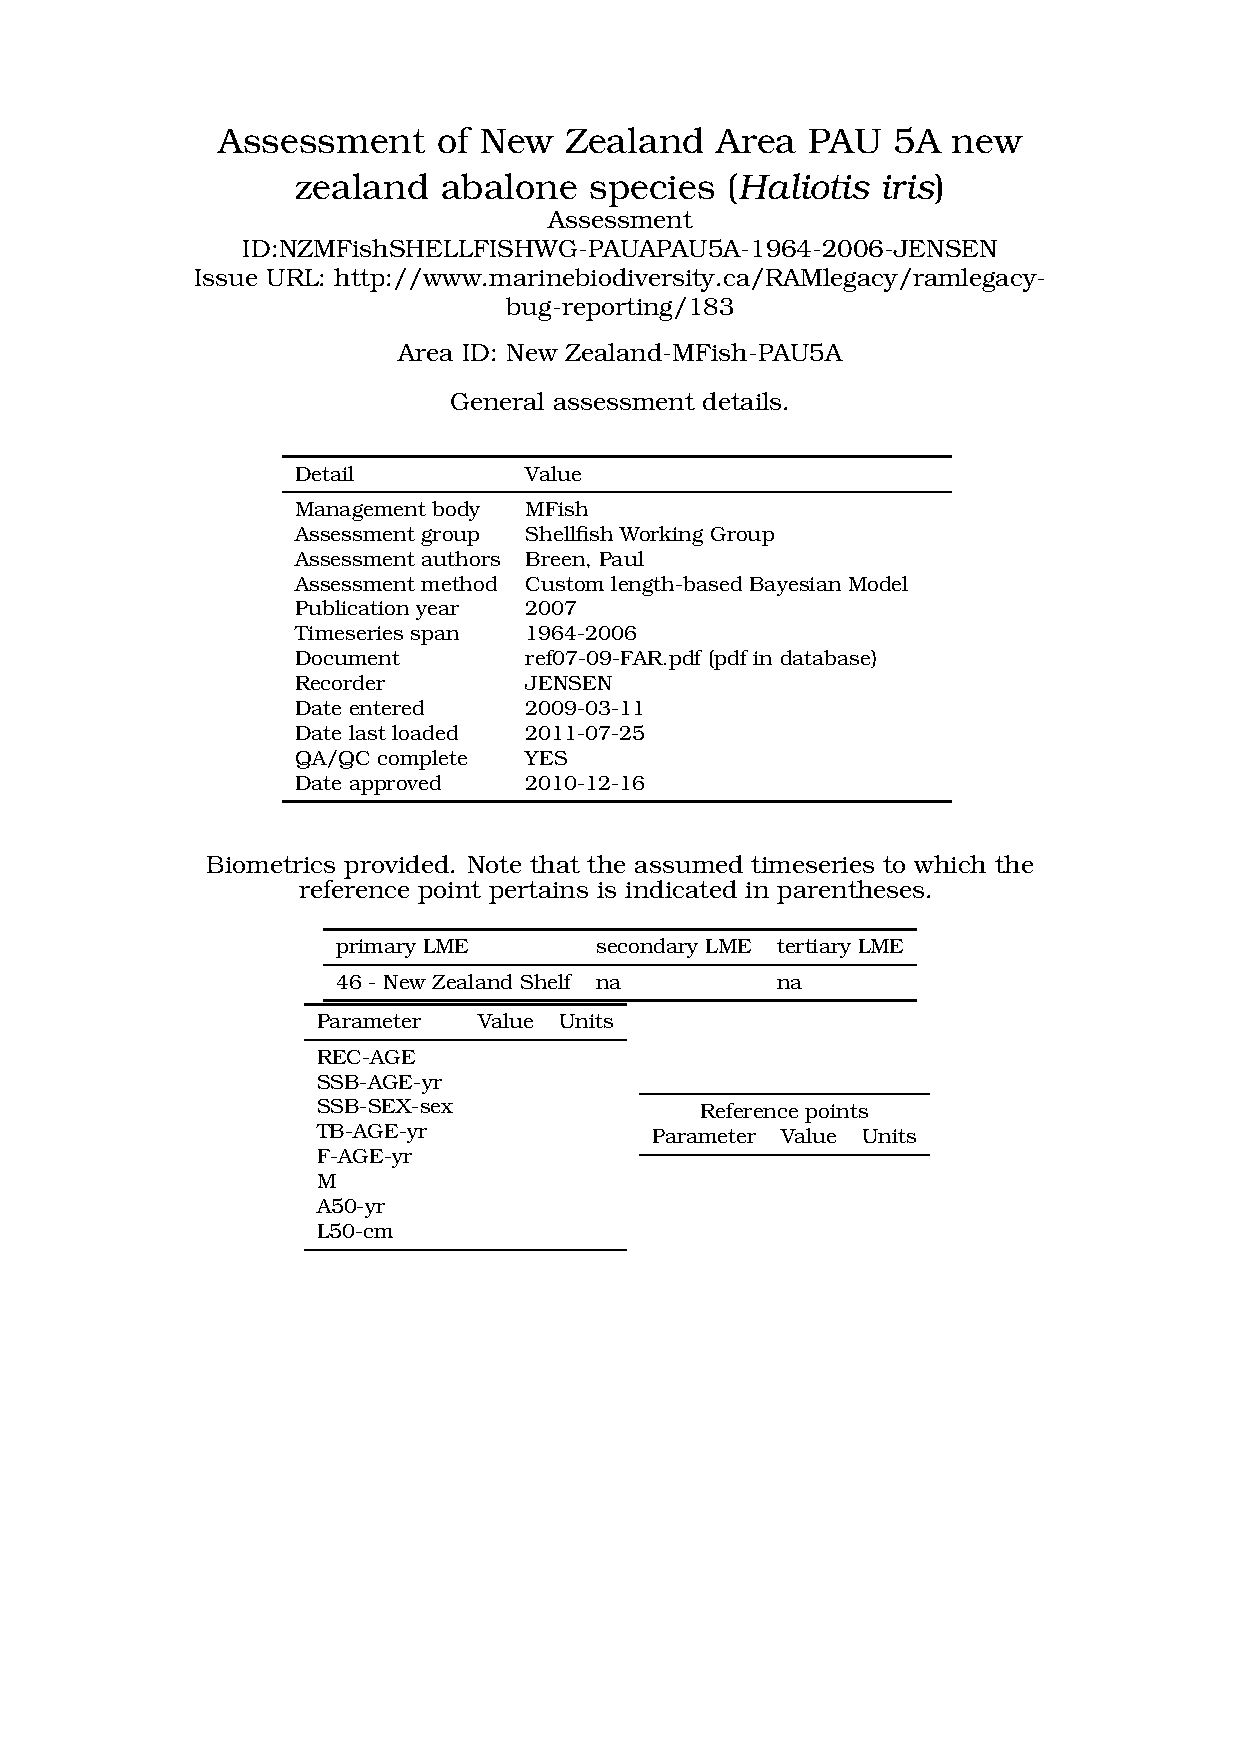
\includepdf[pagecommand={\thispagestyle{plain}}, pages={1,2}]{../../../tex/NZMFishSHELLFISHWG-PAUAPAU5A-1964-2006-JENSEN.pdf}
\index{Blackfoot abalone}\index{Haliotis iris}\index{Haliotididae!Haliotis iris}
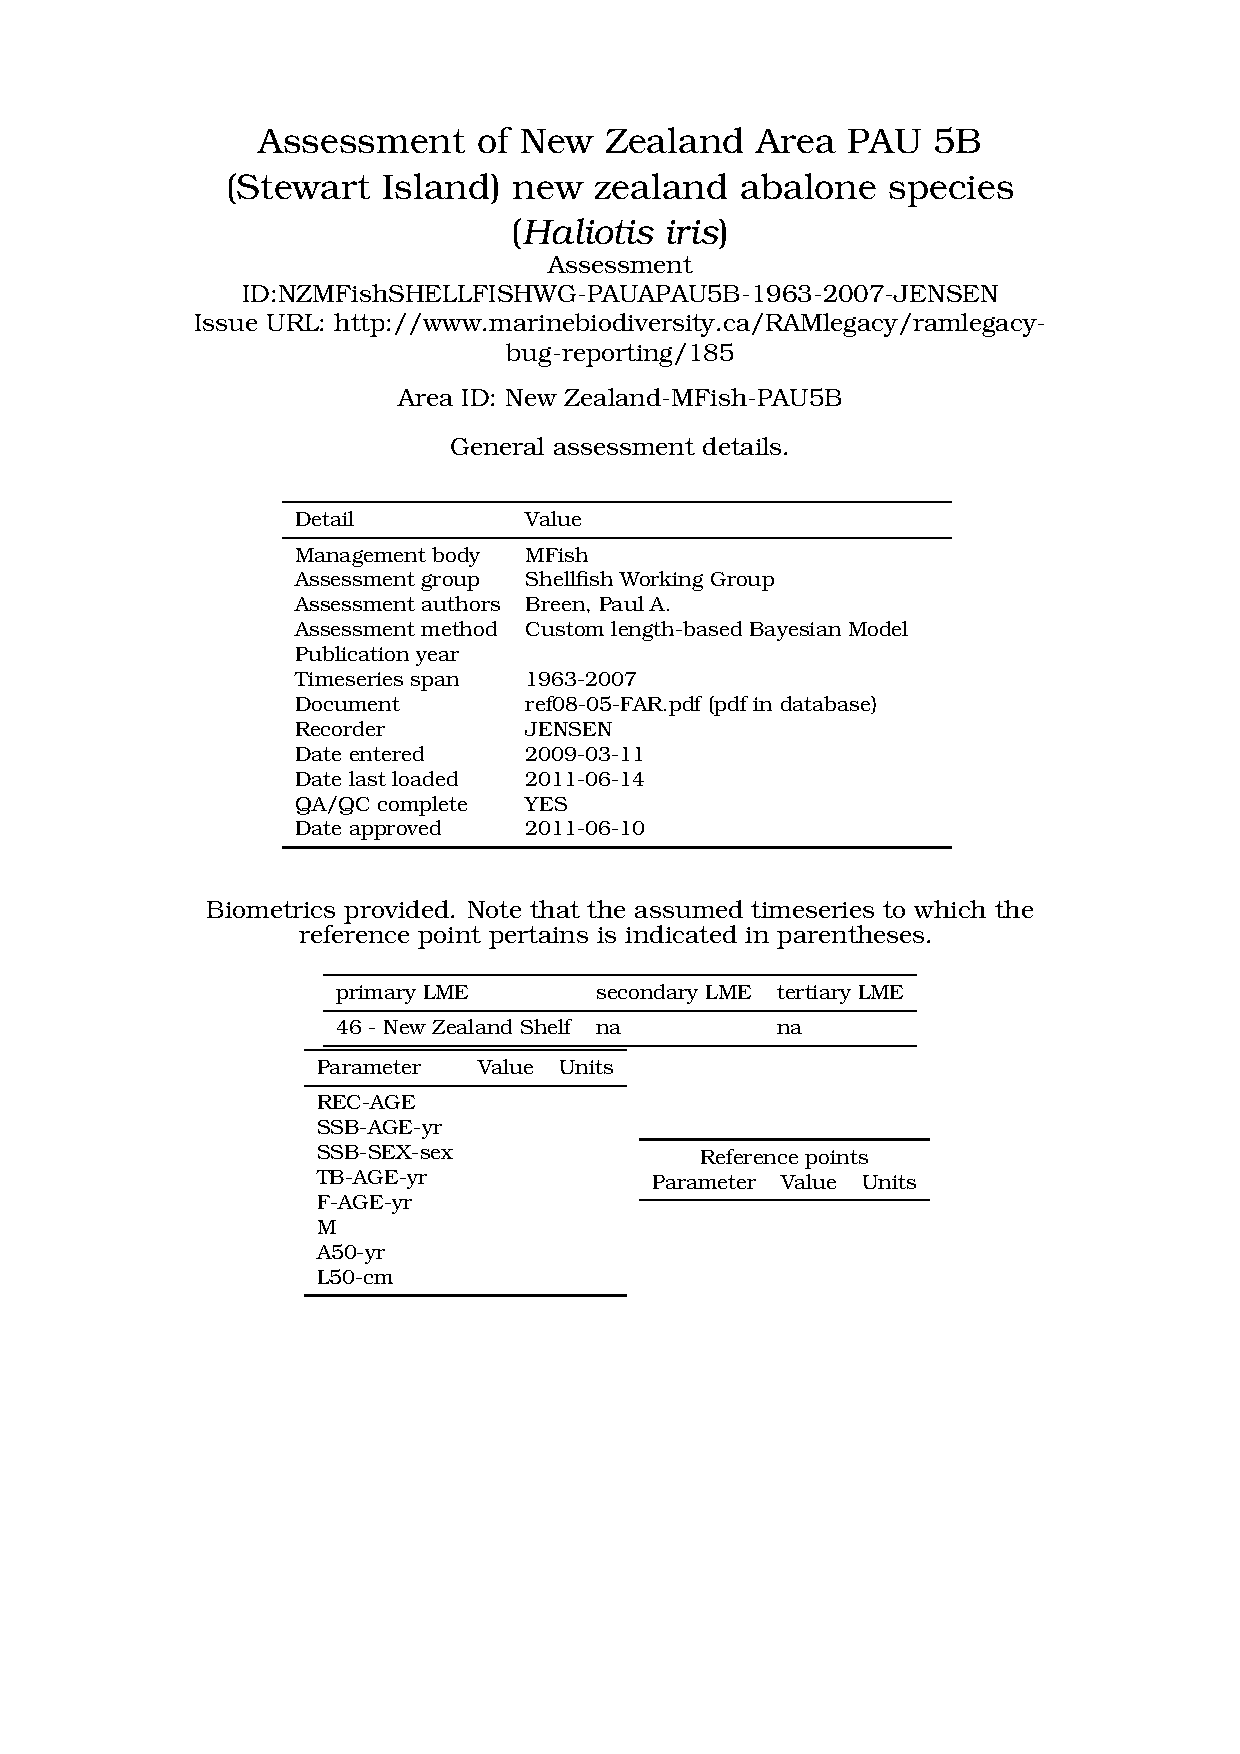
\includepdf[pagecommand={\thispagestyle{plain}}, pages={1,2}]{../../../tex/NZMFishSHELLFISHWG-PAUAPAU5B-1963-2007-JENSEN.pdf}
\index{Blackfoot abalone}\index{Haliotis iris}\index{Haliotididae!Haliotis iris}
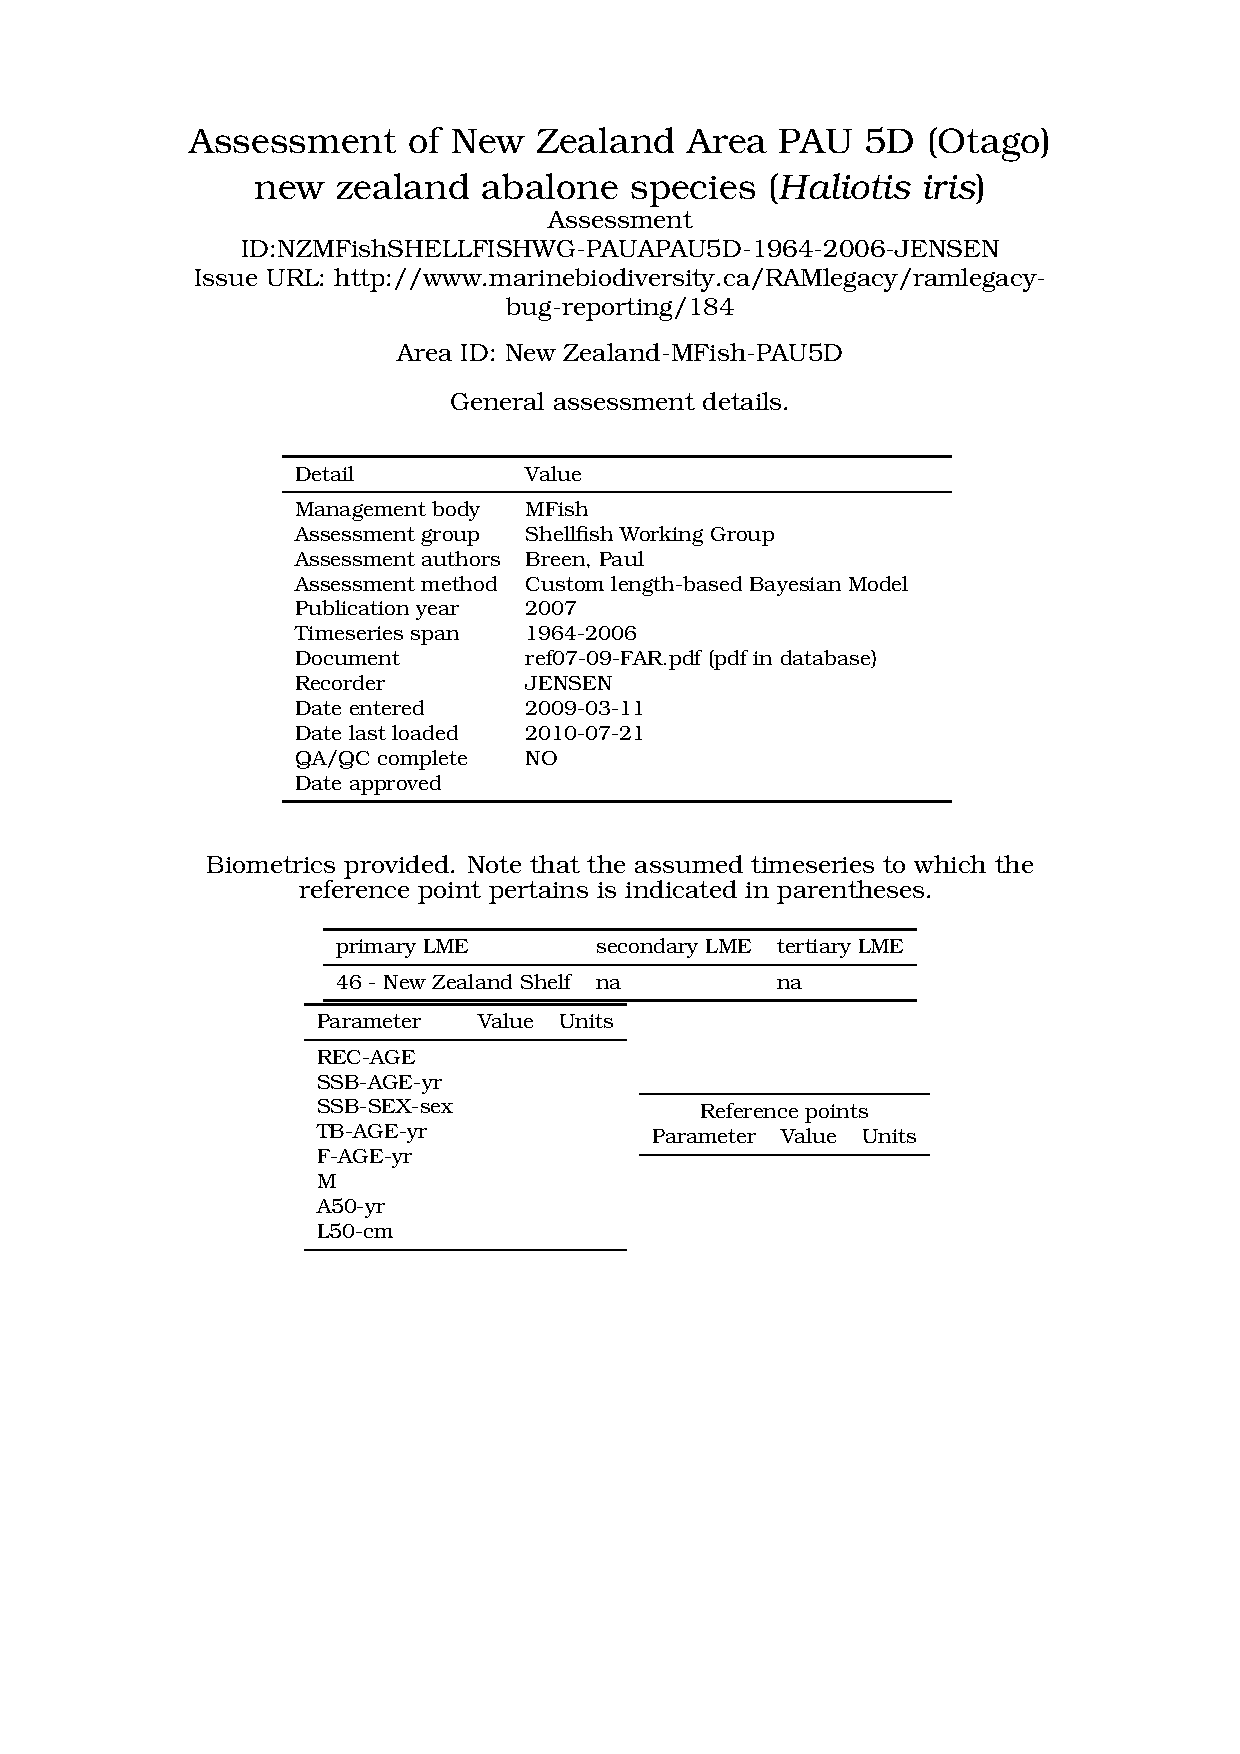
\includepdf[pagecommand={\thispagestyle{plain}}, pages={1,2}]{../../../tex/NZMFishSHELLFISHWG-PAUAPAU5D-1964-2006-JENSEN.pdf}
\index{Blackfoot abalone}\index{Haliotis iris}\index{Haliotididae!Haliotis iris}
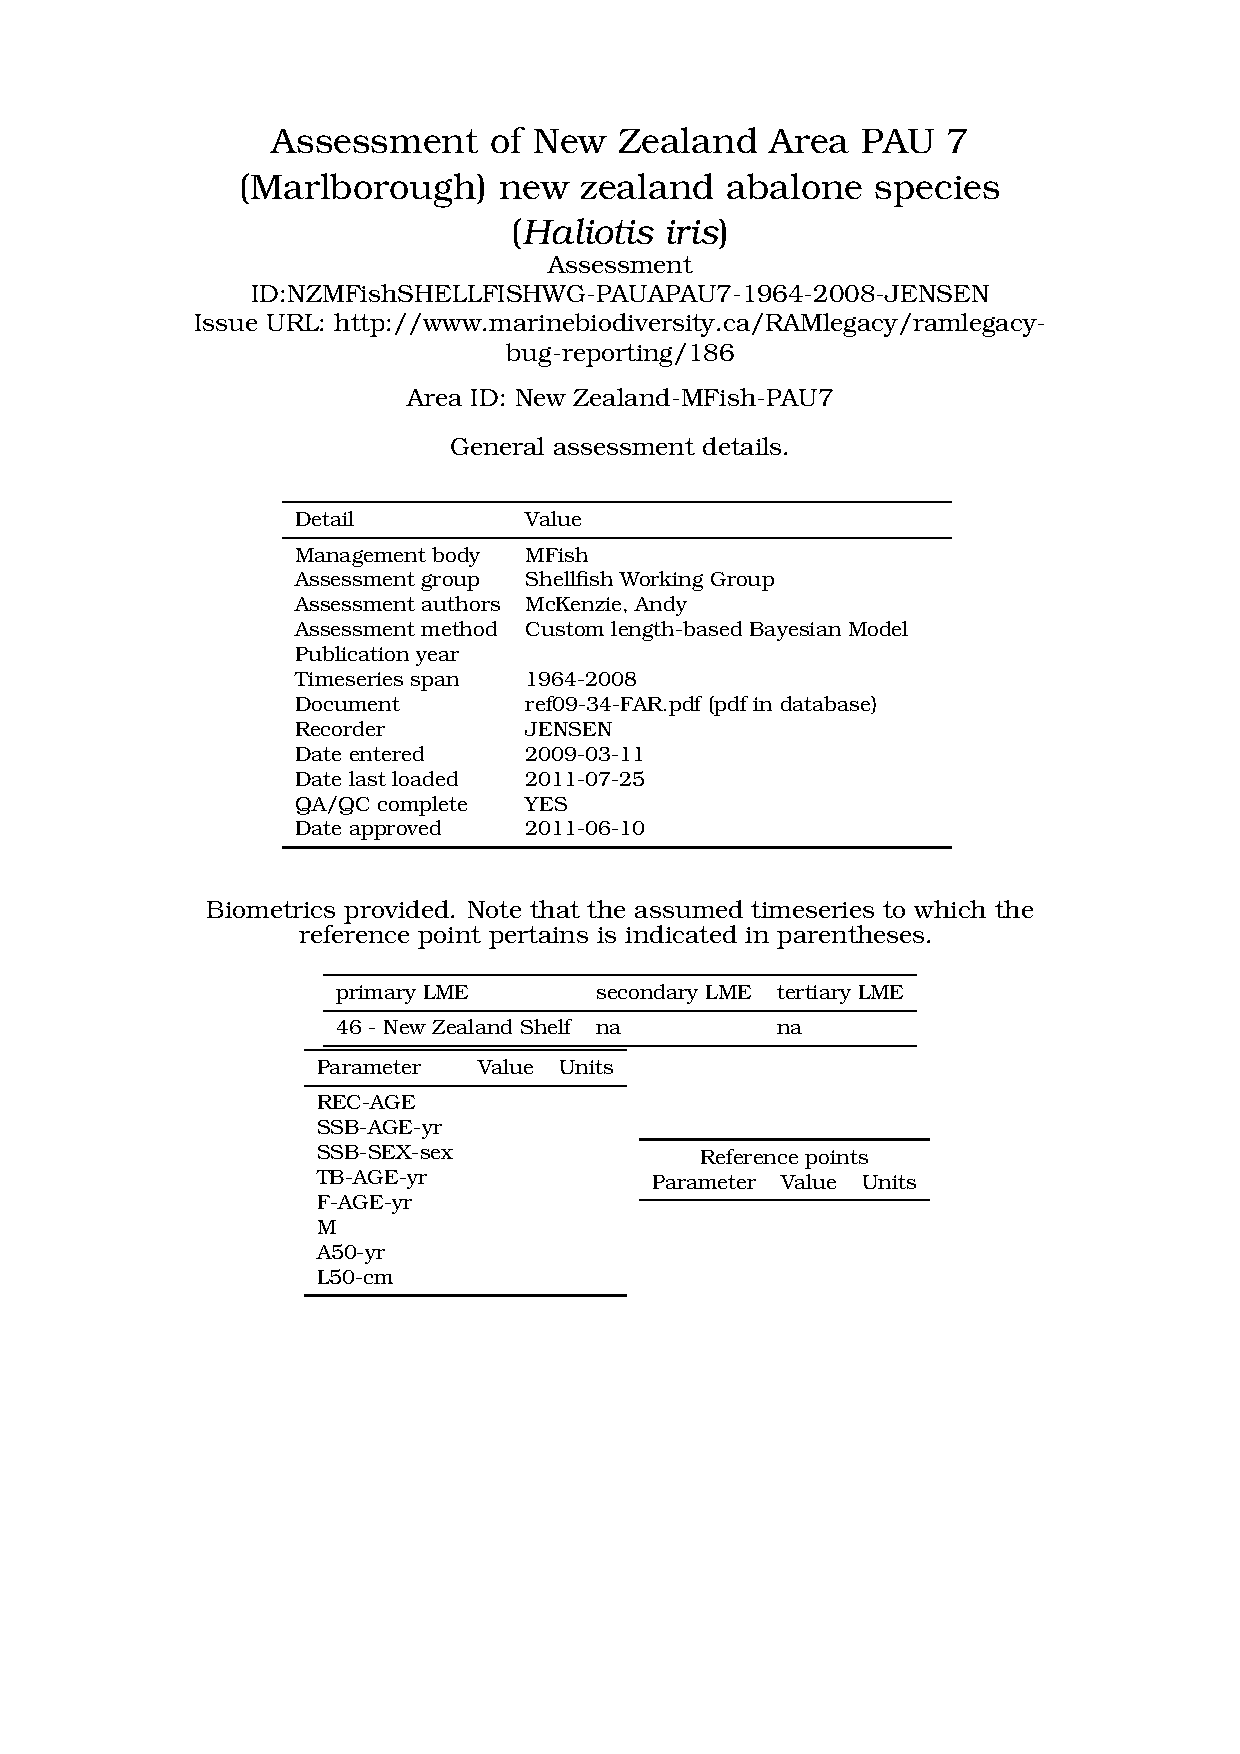
\includepdf[pagecommand={\thispagestyle{plain}}, pages={1,2}]{../../../tex/NZMFishSHELLFISHWG-PAUAPAU7-1964-2008-JENSEN.pdf}
\index{South African abalone}\index{Haliotis midae}\index{Haliotididae!Haliotis midae}
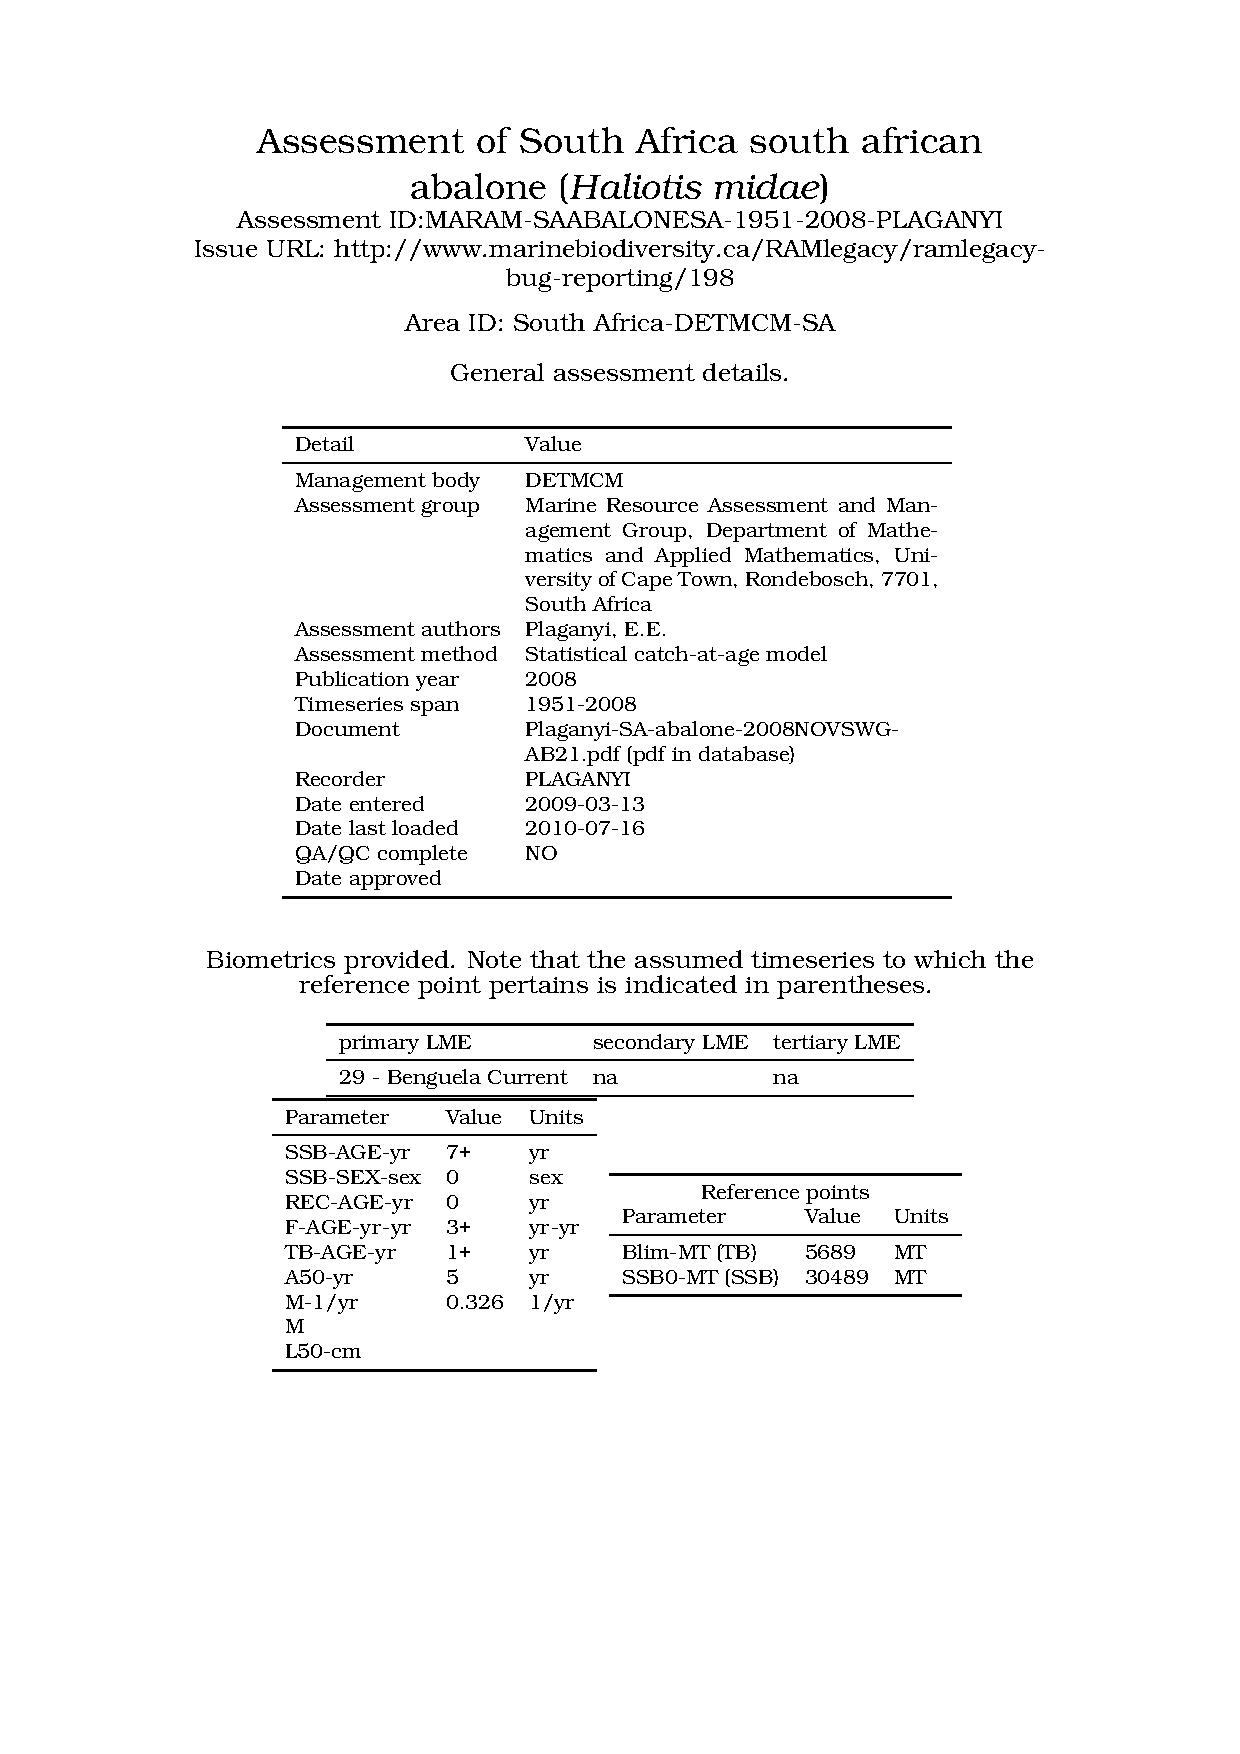
\includepdf[pagecommand={\thispagestyle{plain}}, pages={1,2}]{../../../tex/MARAM-SAABALONESA-1951-2008-PLAGANYI.pdf}
\addcontentsline{toc}{section}{Order Beryciformes}\index{Berycidae}\index{Beryciformes!Berycidae}

\addcontentsline{toc}{subsection}{\hspace{0.2cm}Family Berycidae}\index{Bight redfish}\index{Centroberyx gerrardi}\index{Berycidae!Centroberyx gerrardi}
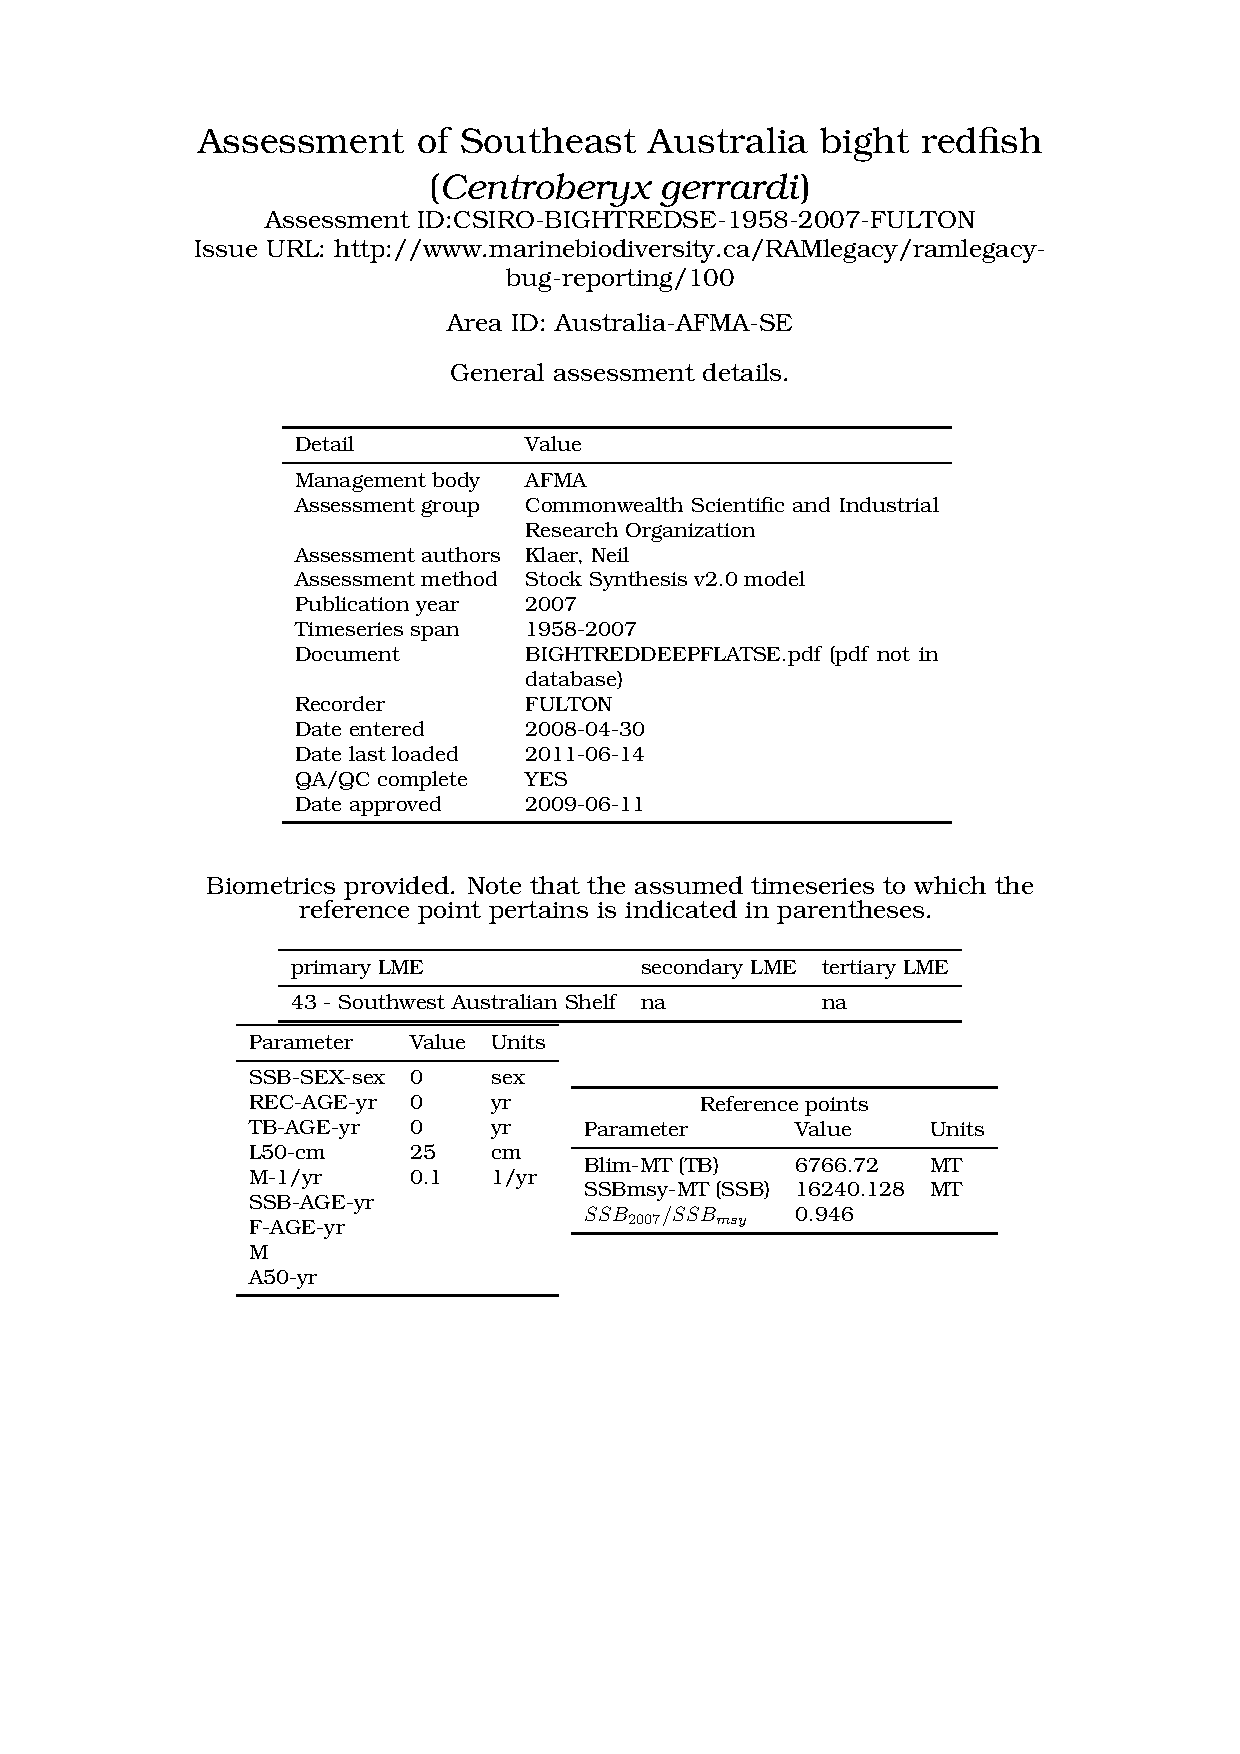
\includepdf[pagecommand={\thispagestyle{plain}}, pages={1,2}]{../../../tex/CSIRO-BIGHTREDSE-1958-2007-FULTON.pdf}
\index{Trachichthyidae}\index{Beryciformes!Trachichthyidae}

\addcontentsline{toc}{subsection}{\hspace{0.2cm}Family Trachichthyidae}\index{Orange roughy}\index{Hoplostethus atlanticus}\index{Trachichthyidae!Hoplostethus atlanticus}
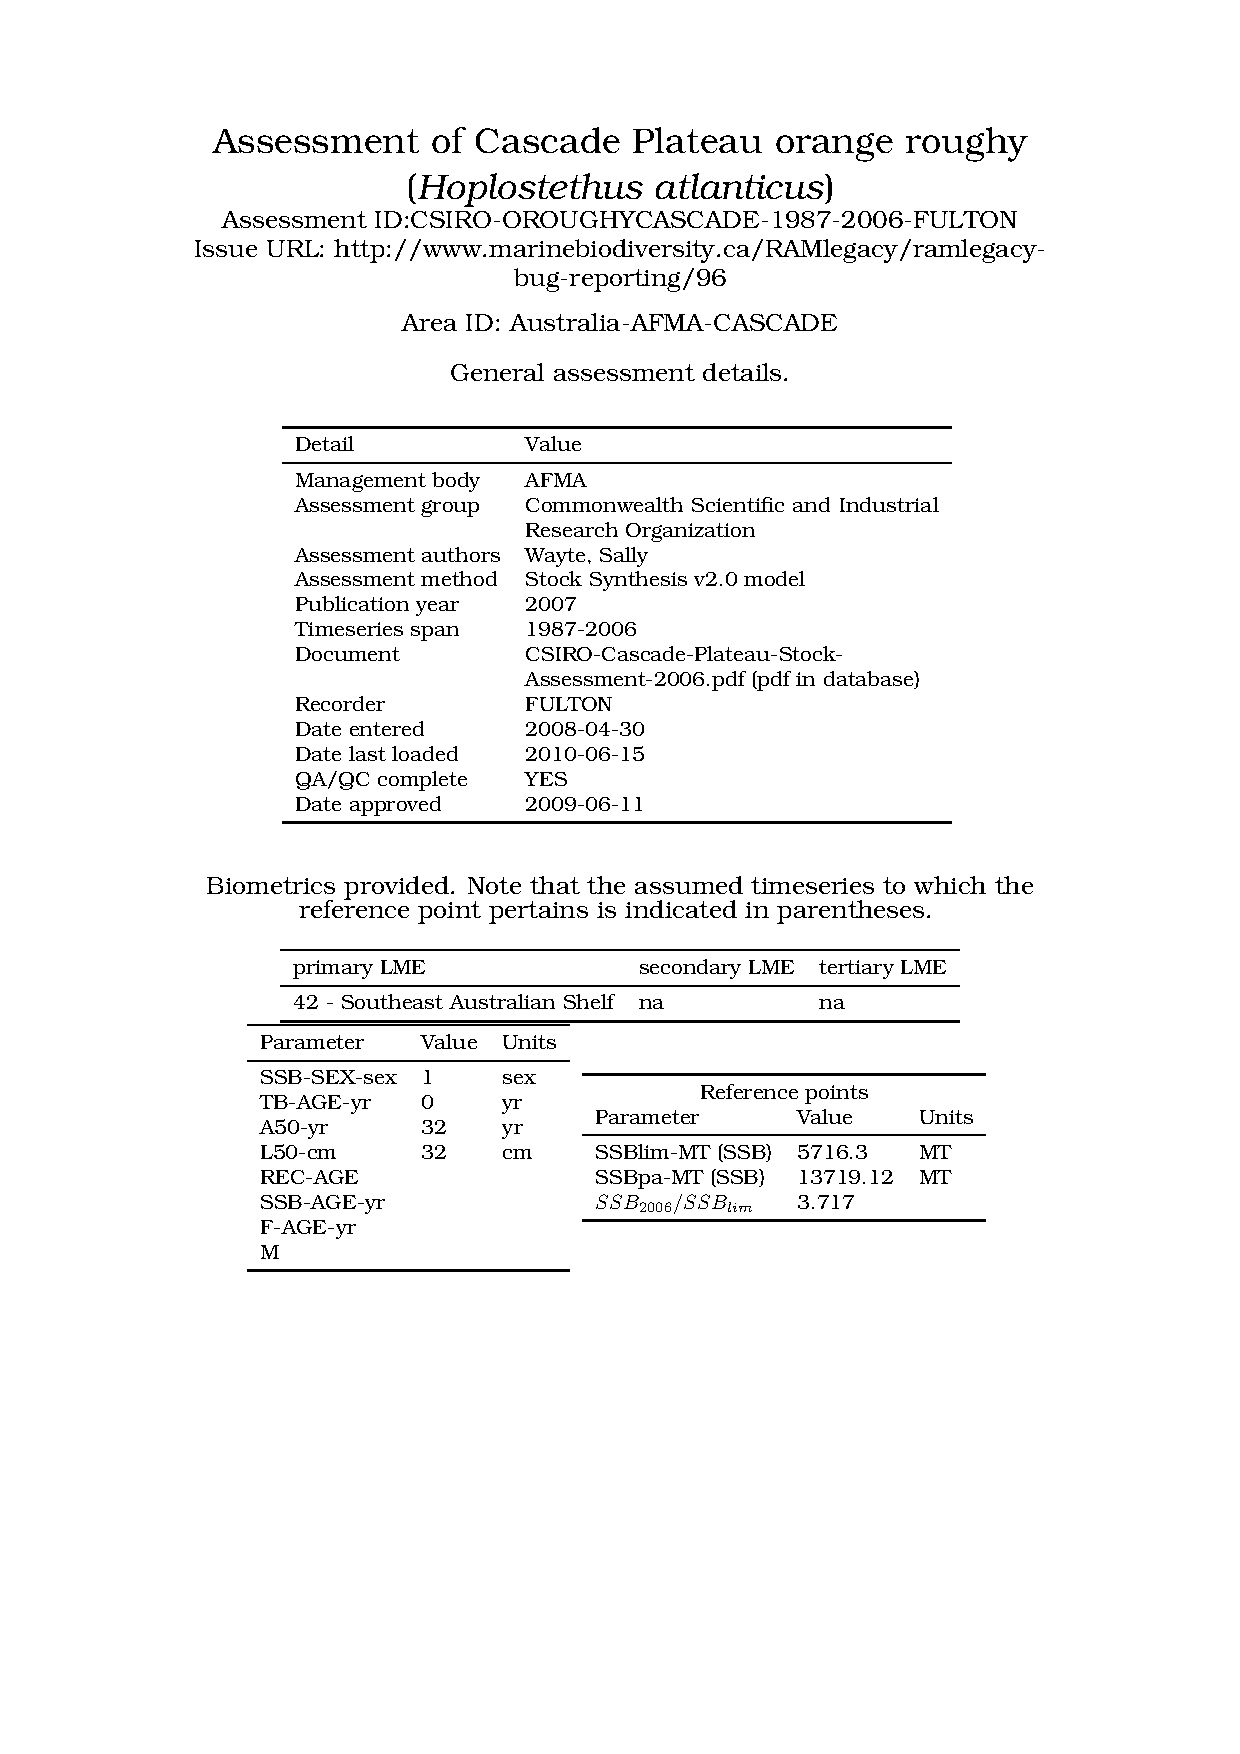
\includepdf[pagecommand={\thispagestyle{plain}}, pages={1,2}]{../../../tex/CSIRO-OROUGHYCASCADE-1987-2006-FULTON.pdf}
\index{Orange roughy}\index{Hoplostethus atlanticus}\index{Trachichthyidae!Hoplostethus atlanticus}
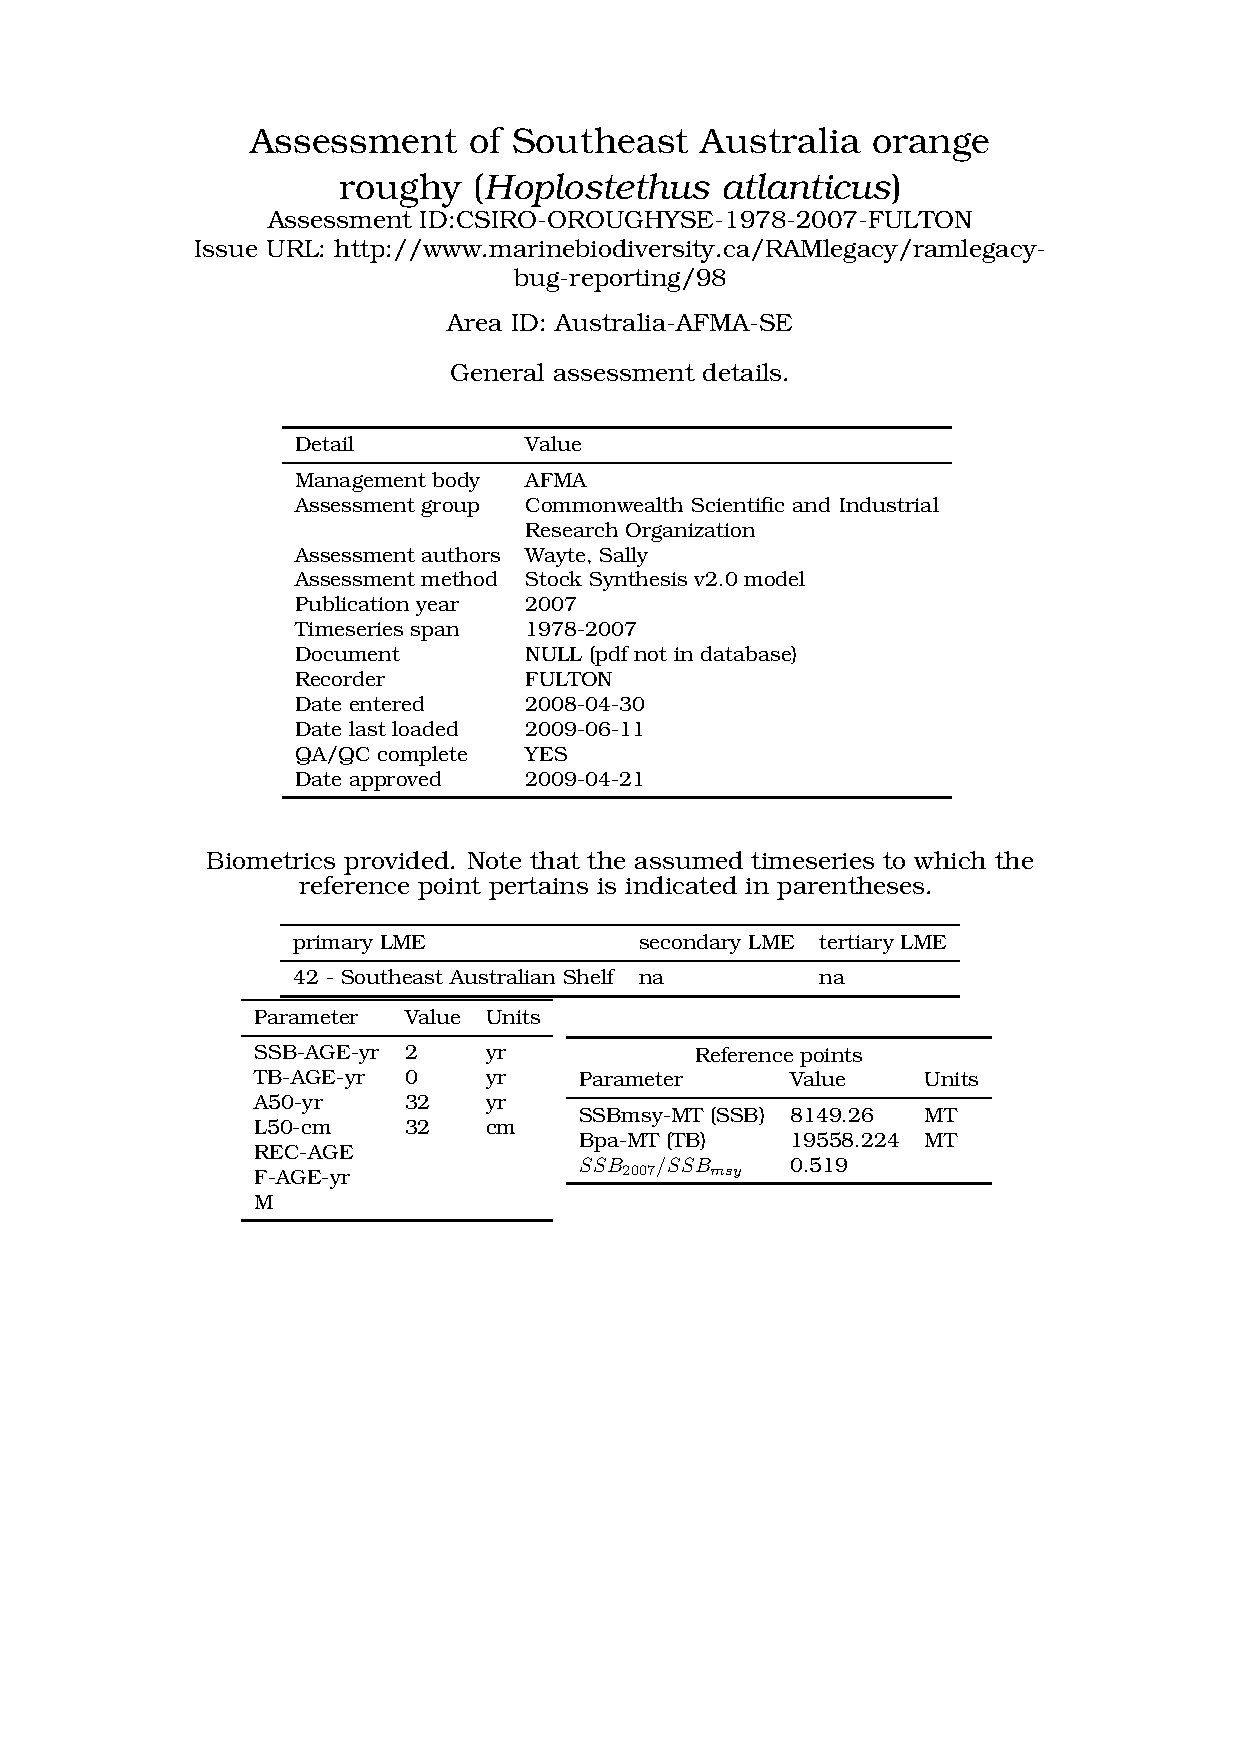
\includepdf[pagecommand={\thispagestyle{plain}}, pages={1,2}]{../../../tex/CSIRO-OROUGHYSE-1978-2007-FULTON.pdf}
\index{Orange roughy}\index{Hoplostethus atlanticus}\index{Trachichthyidae!Hoplostethus atlanticus}
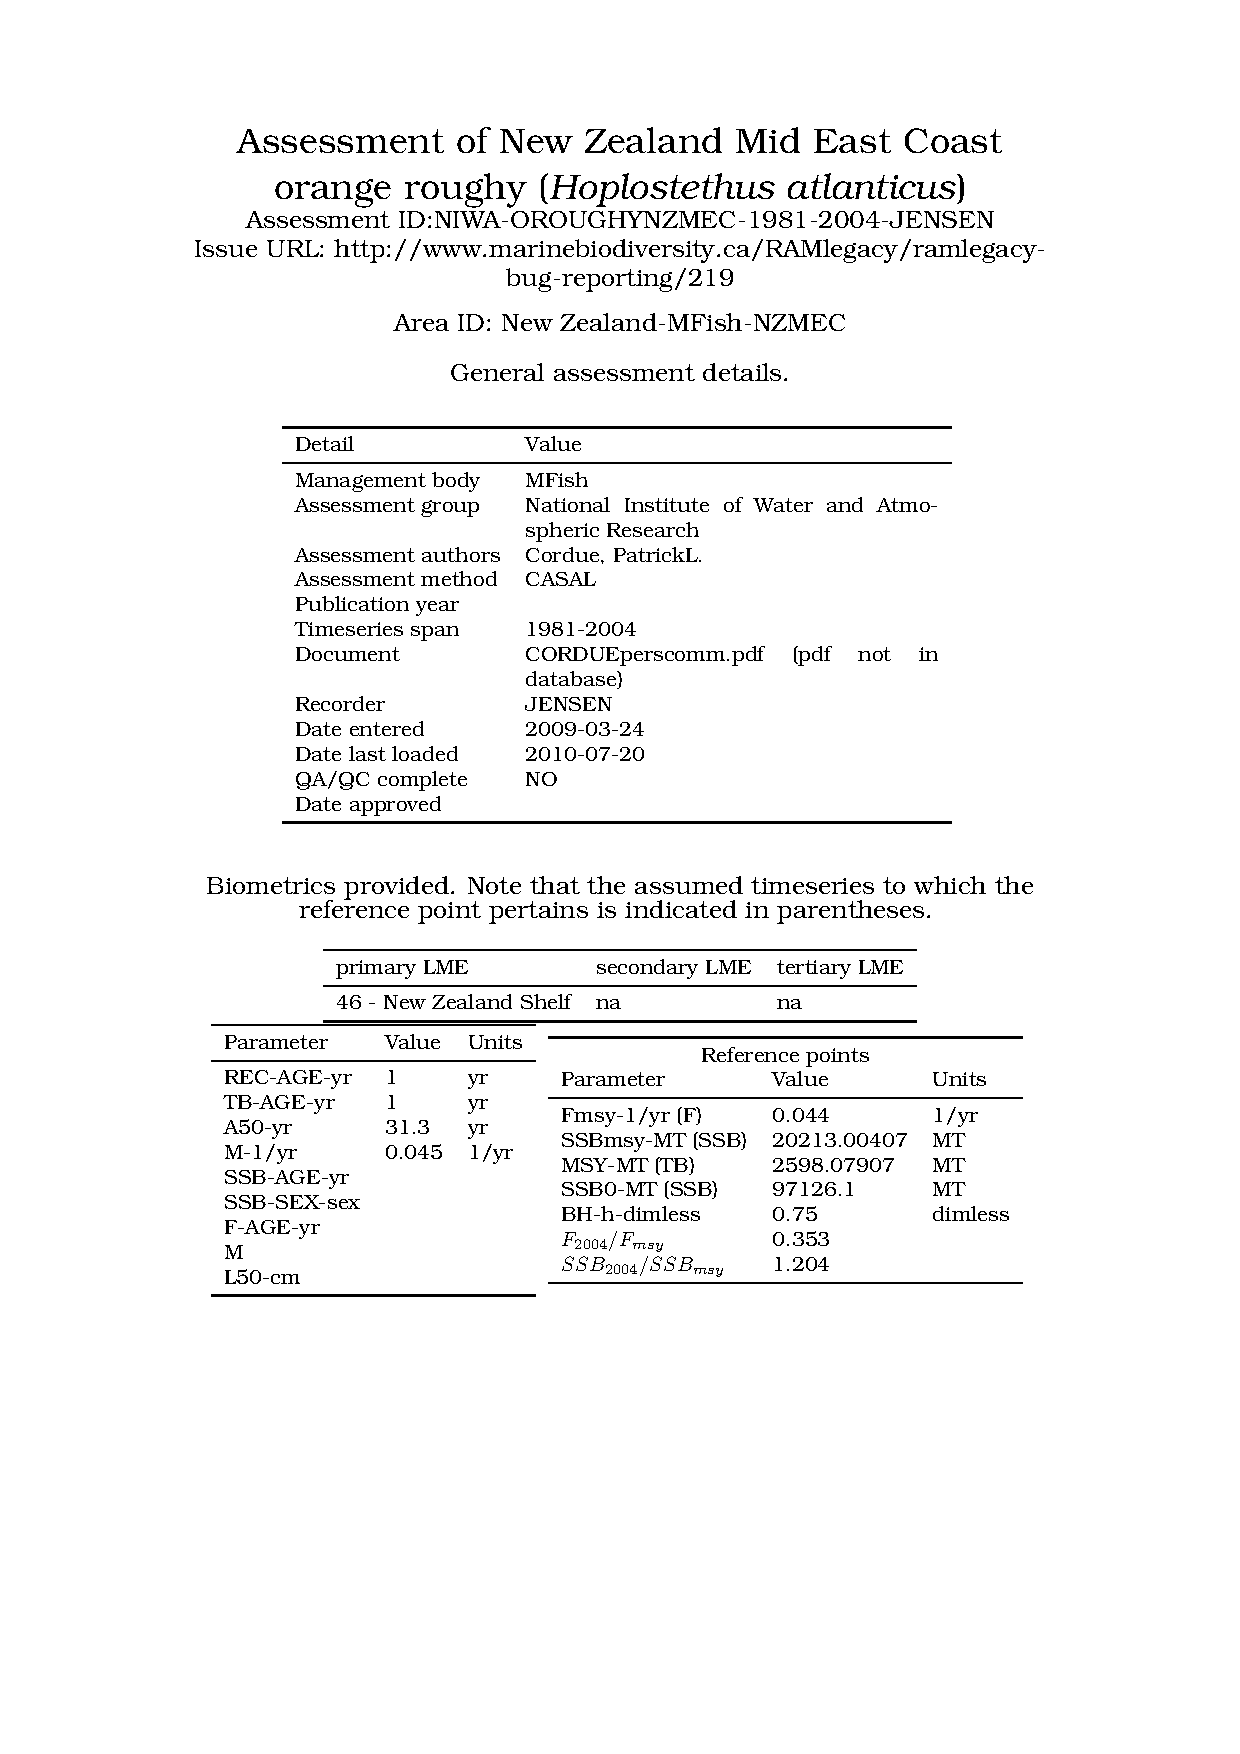
\includepdf[pagecommand={\thispagestyle{plain}}, pages={1,2}]{../../../tex/NIWA-OROUGHYNZMEC-1981-2004-JENSEN.pdf}
\addcontentsline{toc}{section}{Order Carcharhiniformes}\index{Carcharhinidae}\index{Carcharhiniformes!Carcharhinidae}

\addcontentsline{toc}{subsection}{\hspace{0.2cm}Family Carcharhinidae}\index{Blacknose shark}\index{Carcharhinus acronotus}\index{Carcharhinidae!Carcharhinus acronotus}
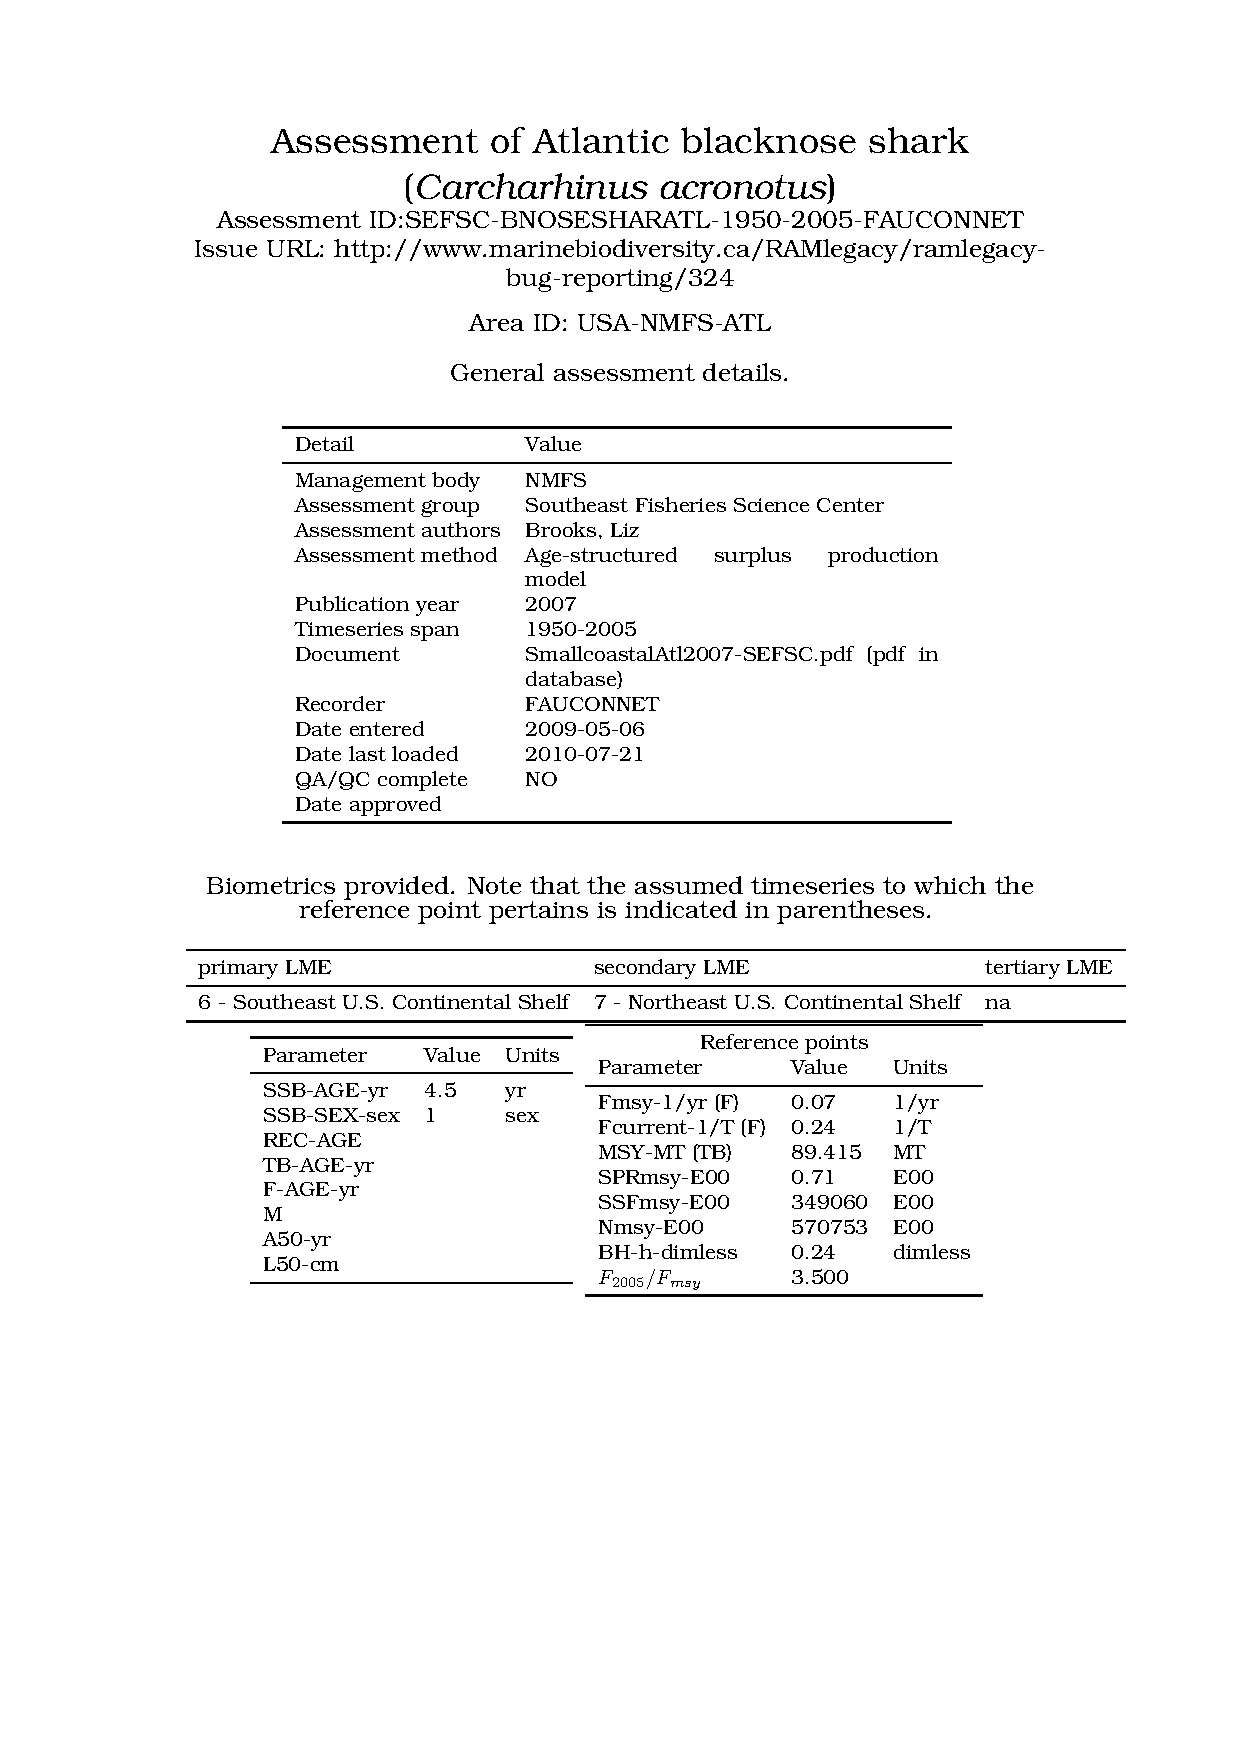
\includepdf[pagecommand={\thispagestyle{plain}}, pages={1,2}]{../../../tex/SEFSC-BNOSESHARATL-1950-2005-FAUCONNET.pdf}
\index{Finetooth shark}\index{Carcharhinus isodon}\index{Carcharhinidae!Carcharhinus isodon}
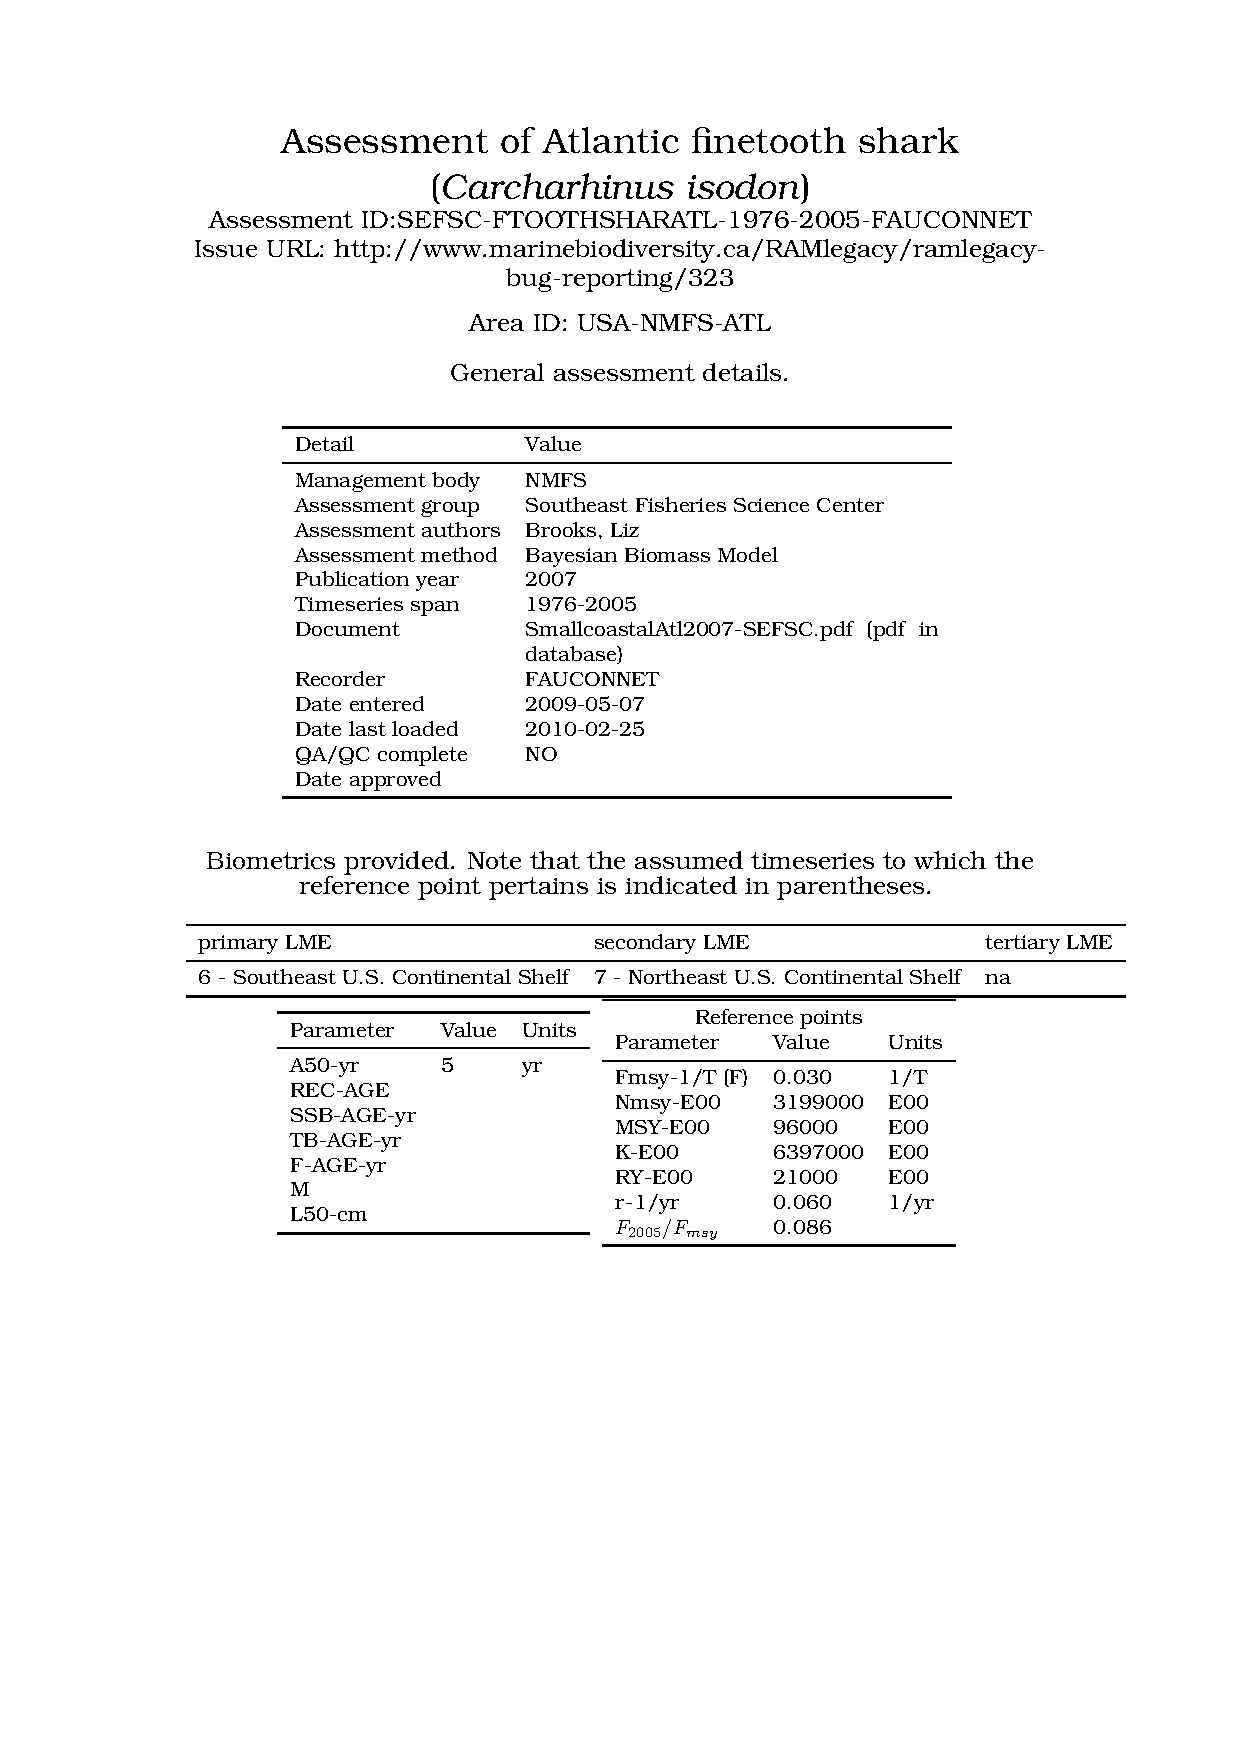
\includepdf[pagecommand={\thispagestyle{plain}}, pages={1,2}]{../../../tex/SEFSC-FTOOTHSHARATL-1976-2005-FAUCONNET.pdf}
\index{Blacktip shark}\index{Carcharhinus limbatus}\index{Carcharhinidae!Carcharhinus limbatus}
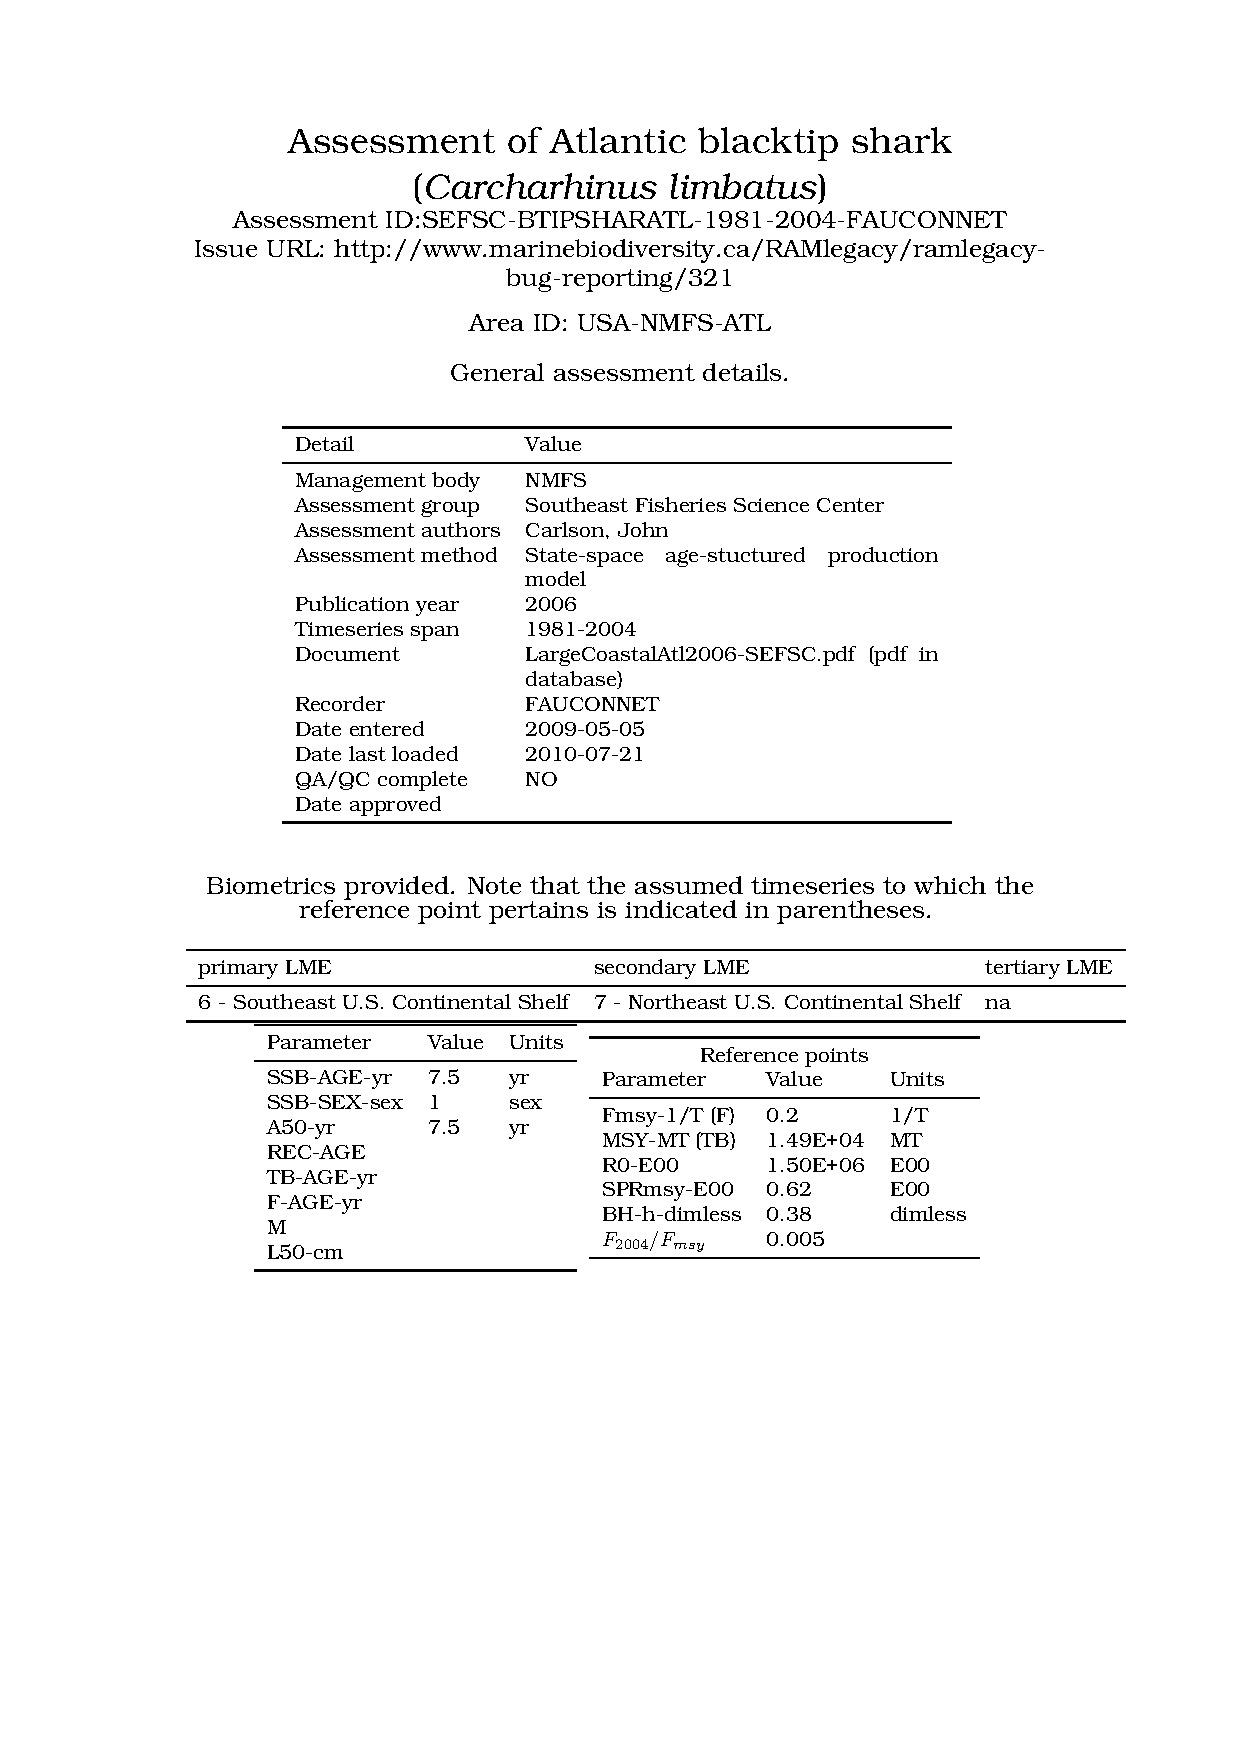
\includepdf[pagecommand={\thispagestyle{plain}}, pages={1,2}]{../../../tex/SEFSC-BTIPSHARATL-1981-2004-FAUCONNET.pdf}
\index{Blacktip shark}\index{Carcharhinus limbatus}\index{Carcharhinidae!Carcharhinus limbatus}
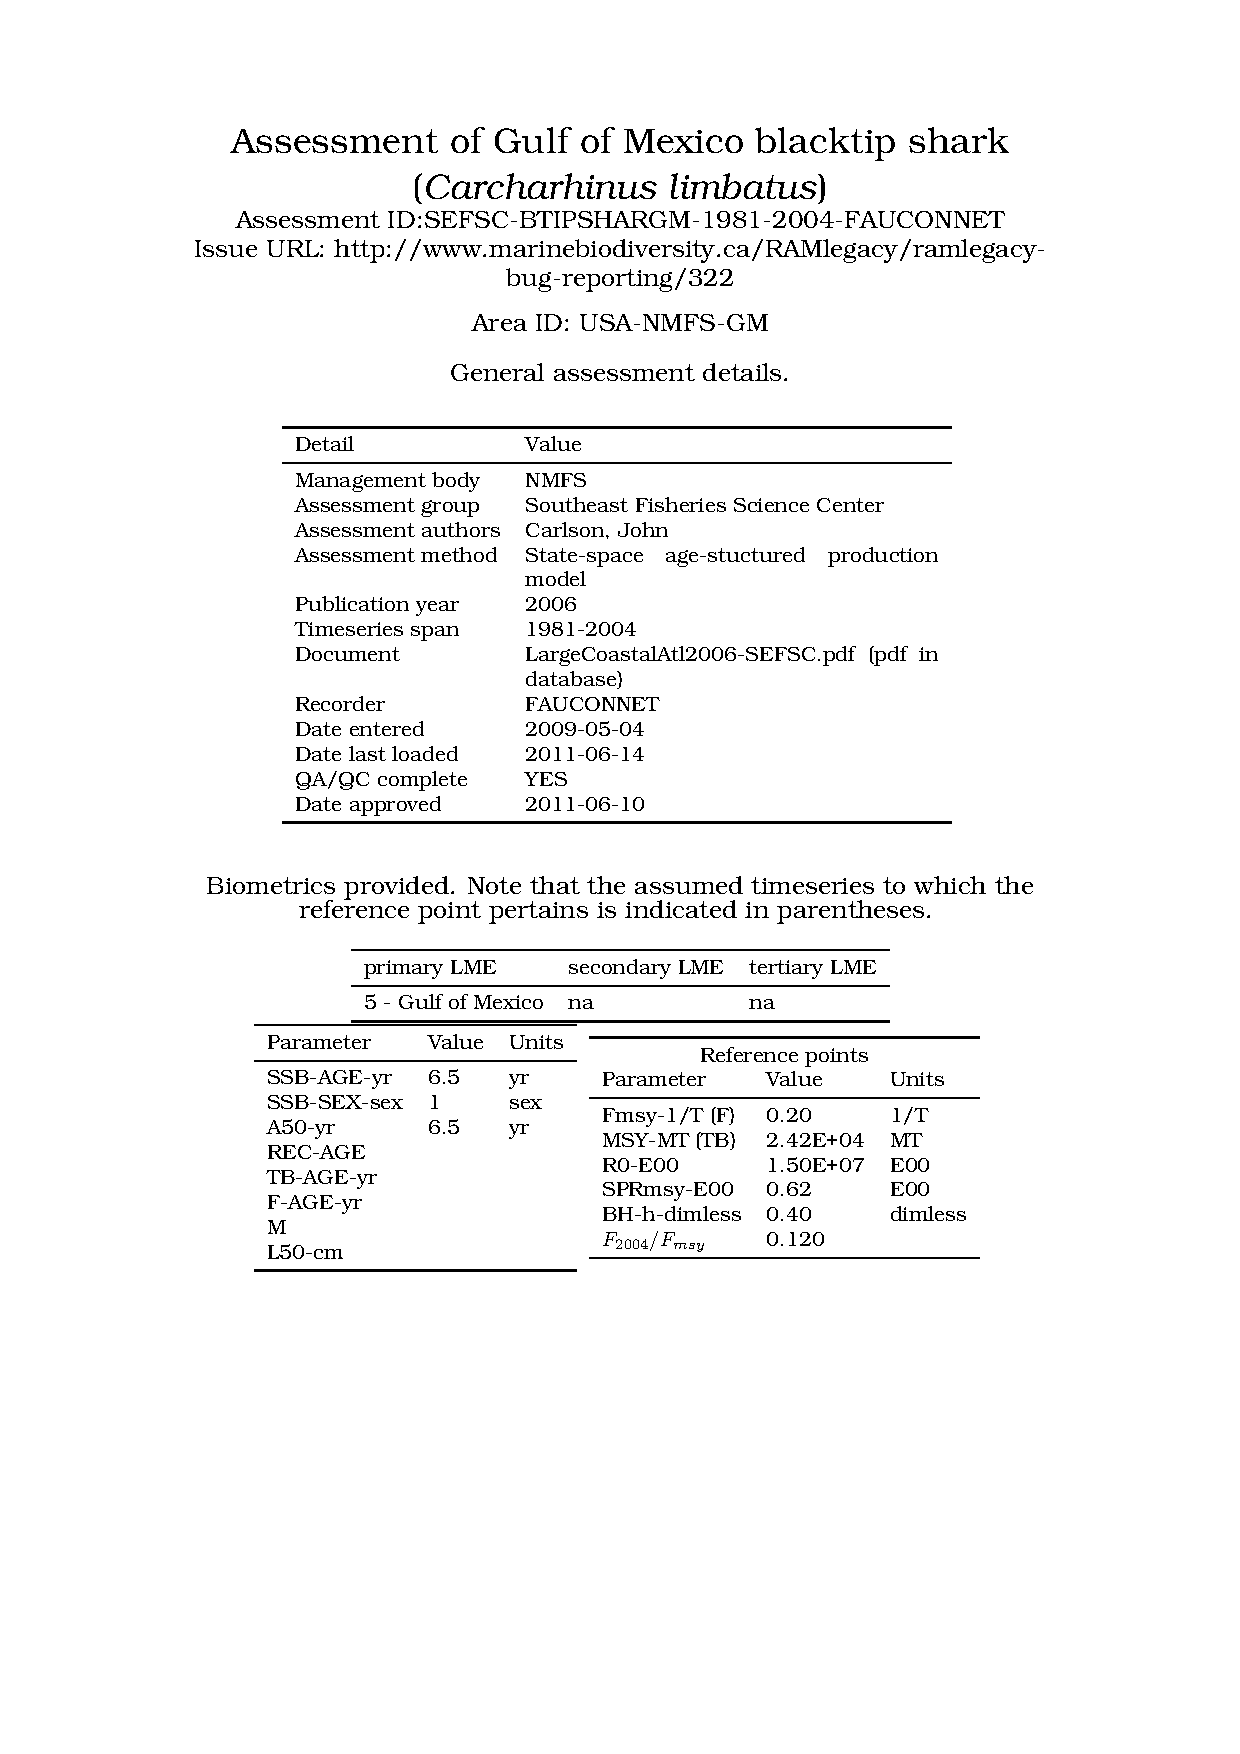
\includepdf[pagecommand={\thispagestyle{plain}}, pages={1,2}]{../../../tex/SEFSC-BTIPSHARGM-1981-2004-FAUCONNET.pdf}
\index{Sandbar shark}\index{Carcharhinus plumbeus}\index{Carcharhinidae!Carcharhinus plumbeus}
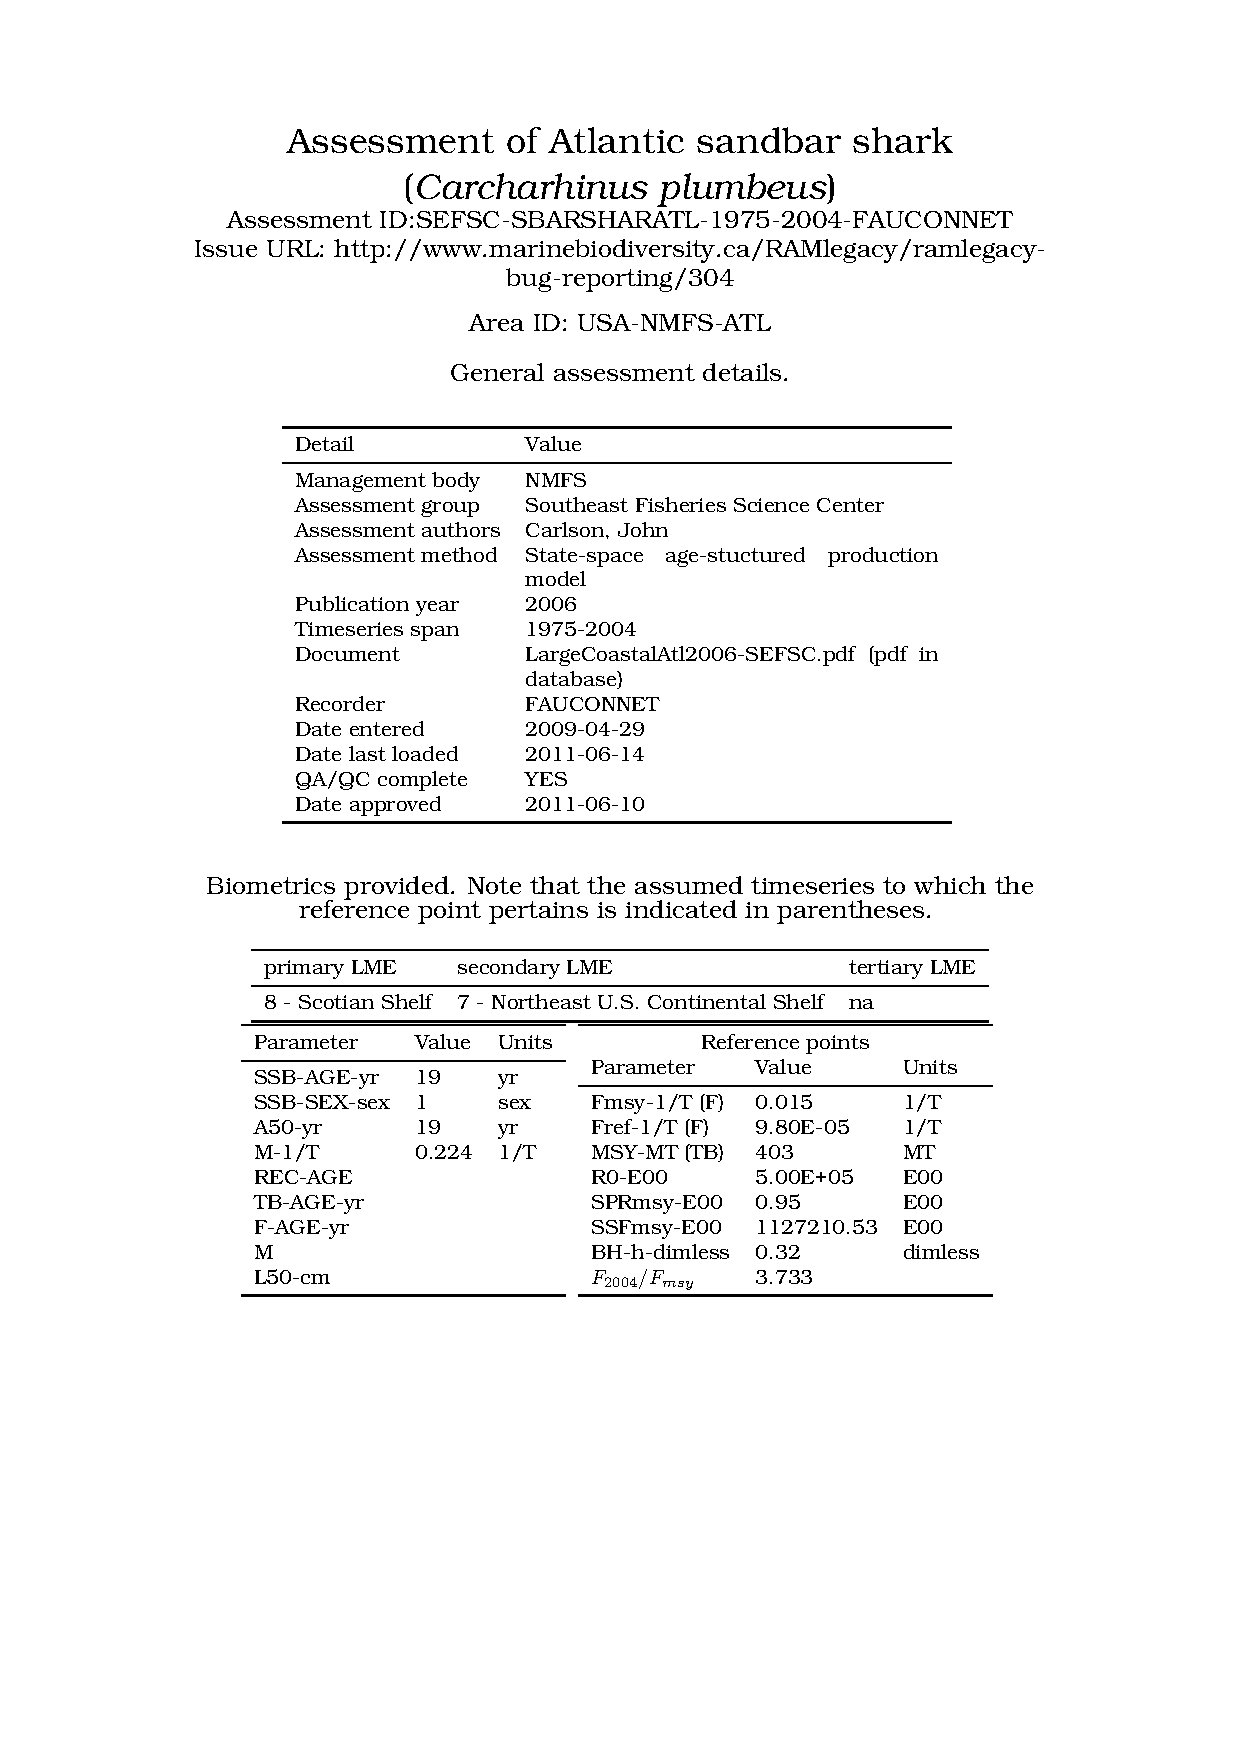
\includepdf[pagecommand={\thispagestyle{plain}}, pages={1,2}]{../../../tex/SEFSC-SBARSHARATL-1975-2004-FAUCONNET.pdf}
\index{Atlantic sharpnose shark}\index{Rhizoprionodon terraenovae}\index{Carcharhinidae!Rhizoprionodon terraenovae}
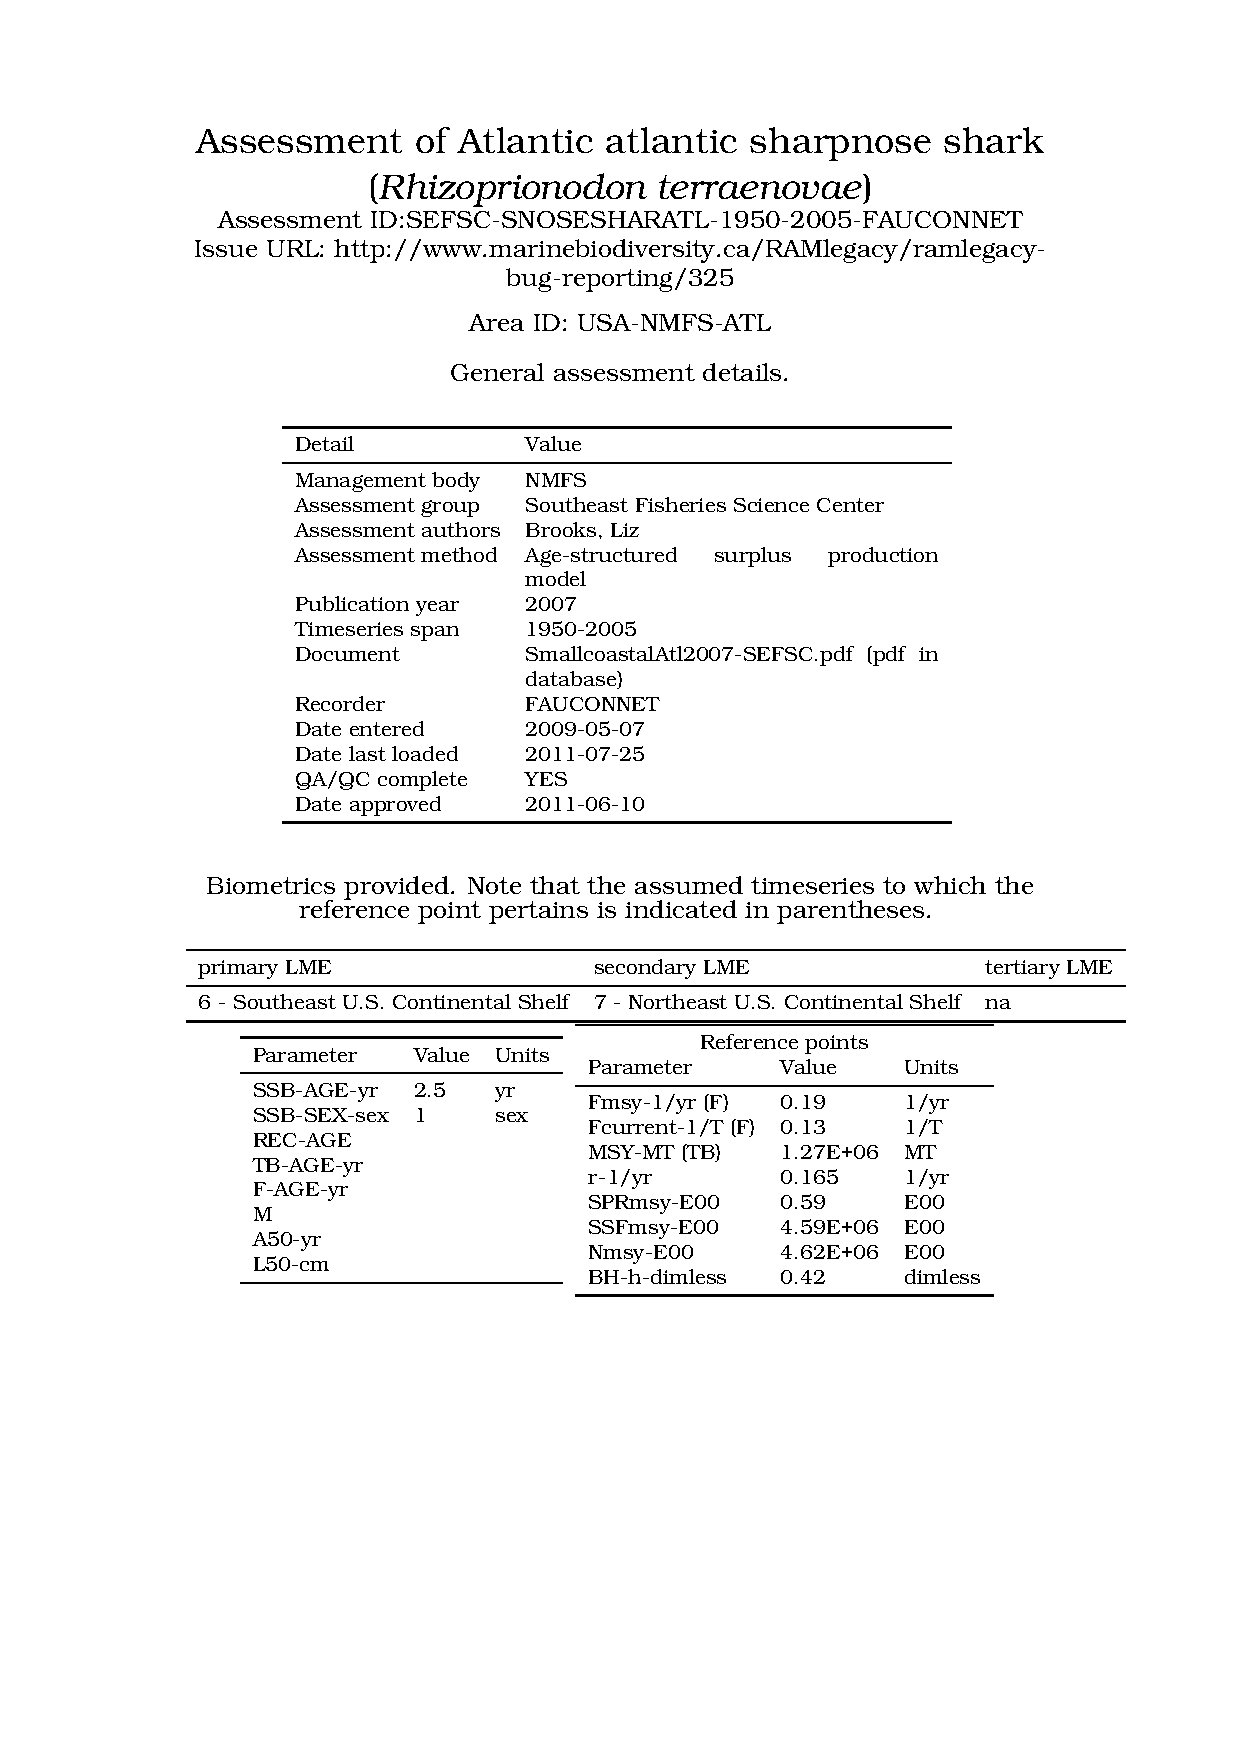
\includepdf[pagecommand={\thispagestyle{plain}}, pages={1,2}]{../../../tex/SEFSC-SNOSESHARATL-1950-2005-FAUCONNET.pdf}
\index{Sphyrnidae}\index{Carcharhiniformes!Sphyrnidae}

\addcontentsline{toc}{subsection}{\hspace{0.2cm}Family Sphyrnidae}\index{Bonnethead shark}\index{Sphyrna tiburo}\index{Sphyrnidae!Sphyrna tiburo}
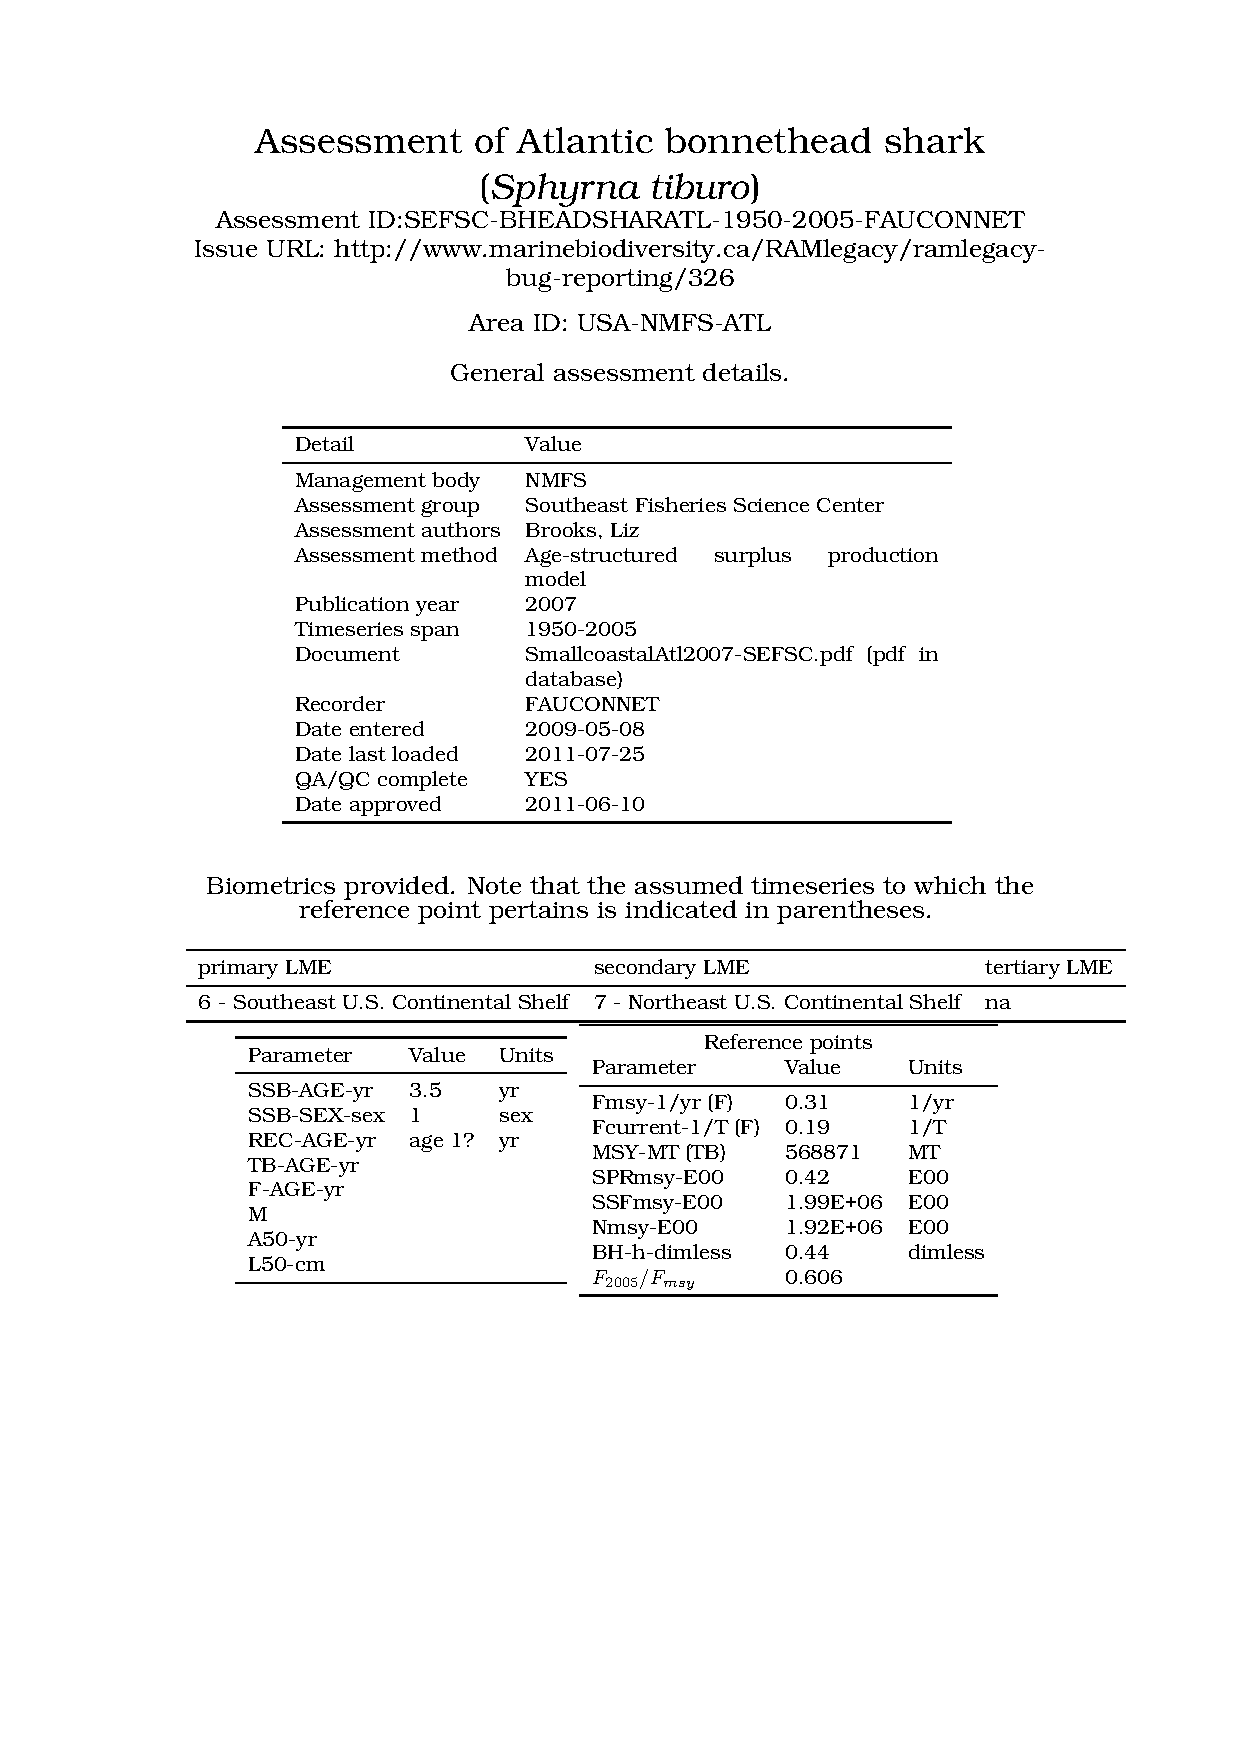
\includepdf[pagecommand={\thispagestyle{plain}}, pages={1,2}]{../../../tex/SEFSC-BHEADSHARATL-1950-2005-FAUCONNET.pdf}
\addcontentsline{toc}{section}{Order Clupeiformes}\index{Clupeidae}\index{Clupeiformes!Clupeidae}

\addcontentsline{toc}{subsection}{\hspace{0.2cm}Family Clupeidae}\index{Gulf menhaden}\index{Brevoortia patronus}\index{Clupeidae!Brevoortia patronus}
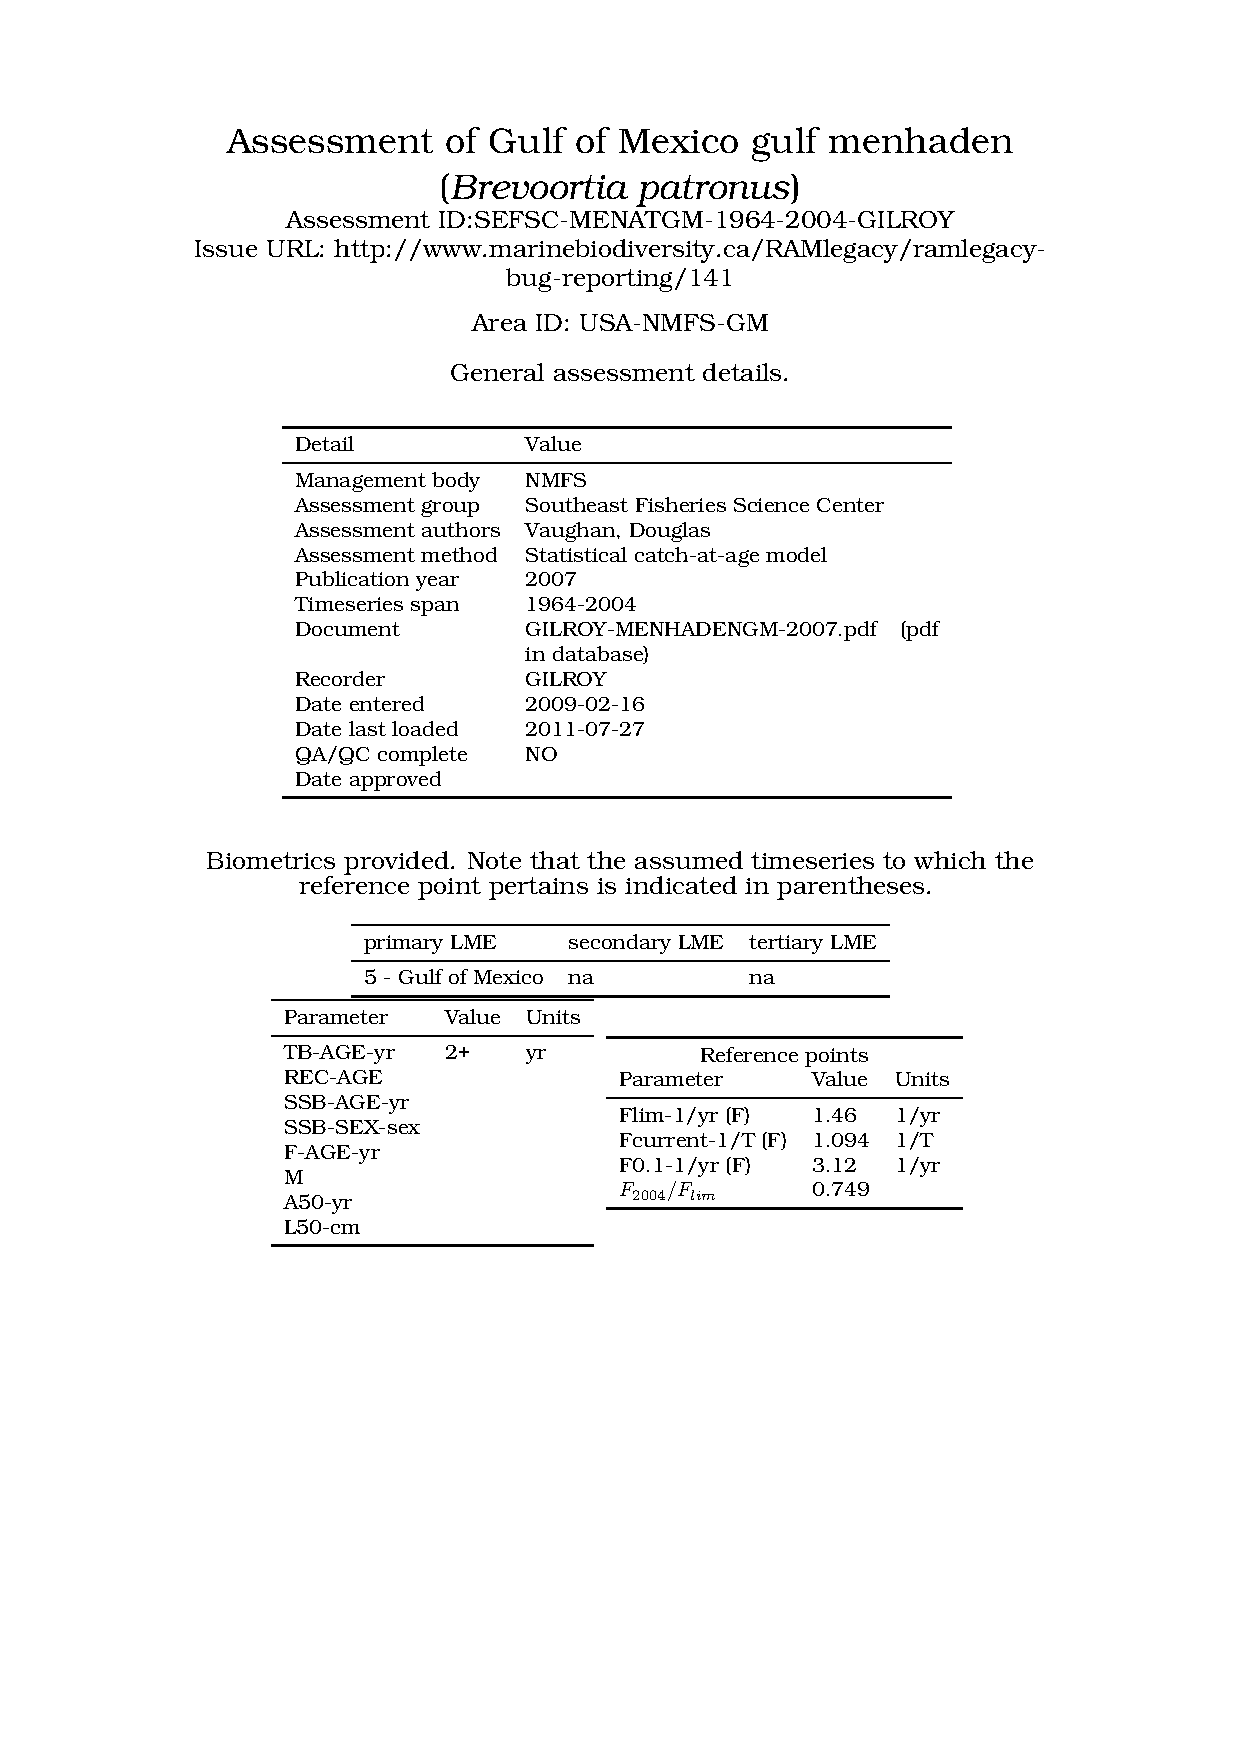
\includepdf[pagecommand={\thispagestyle{plain}}, pages={1,2}]{../../../tex/SEFSC-MENATGM-1964-2004-GILROY.pdf}
\index{Atlantic menhaden}\index{Brevoortia tyrannus}\index{Clupeidae!Brevoortia tyrannus}
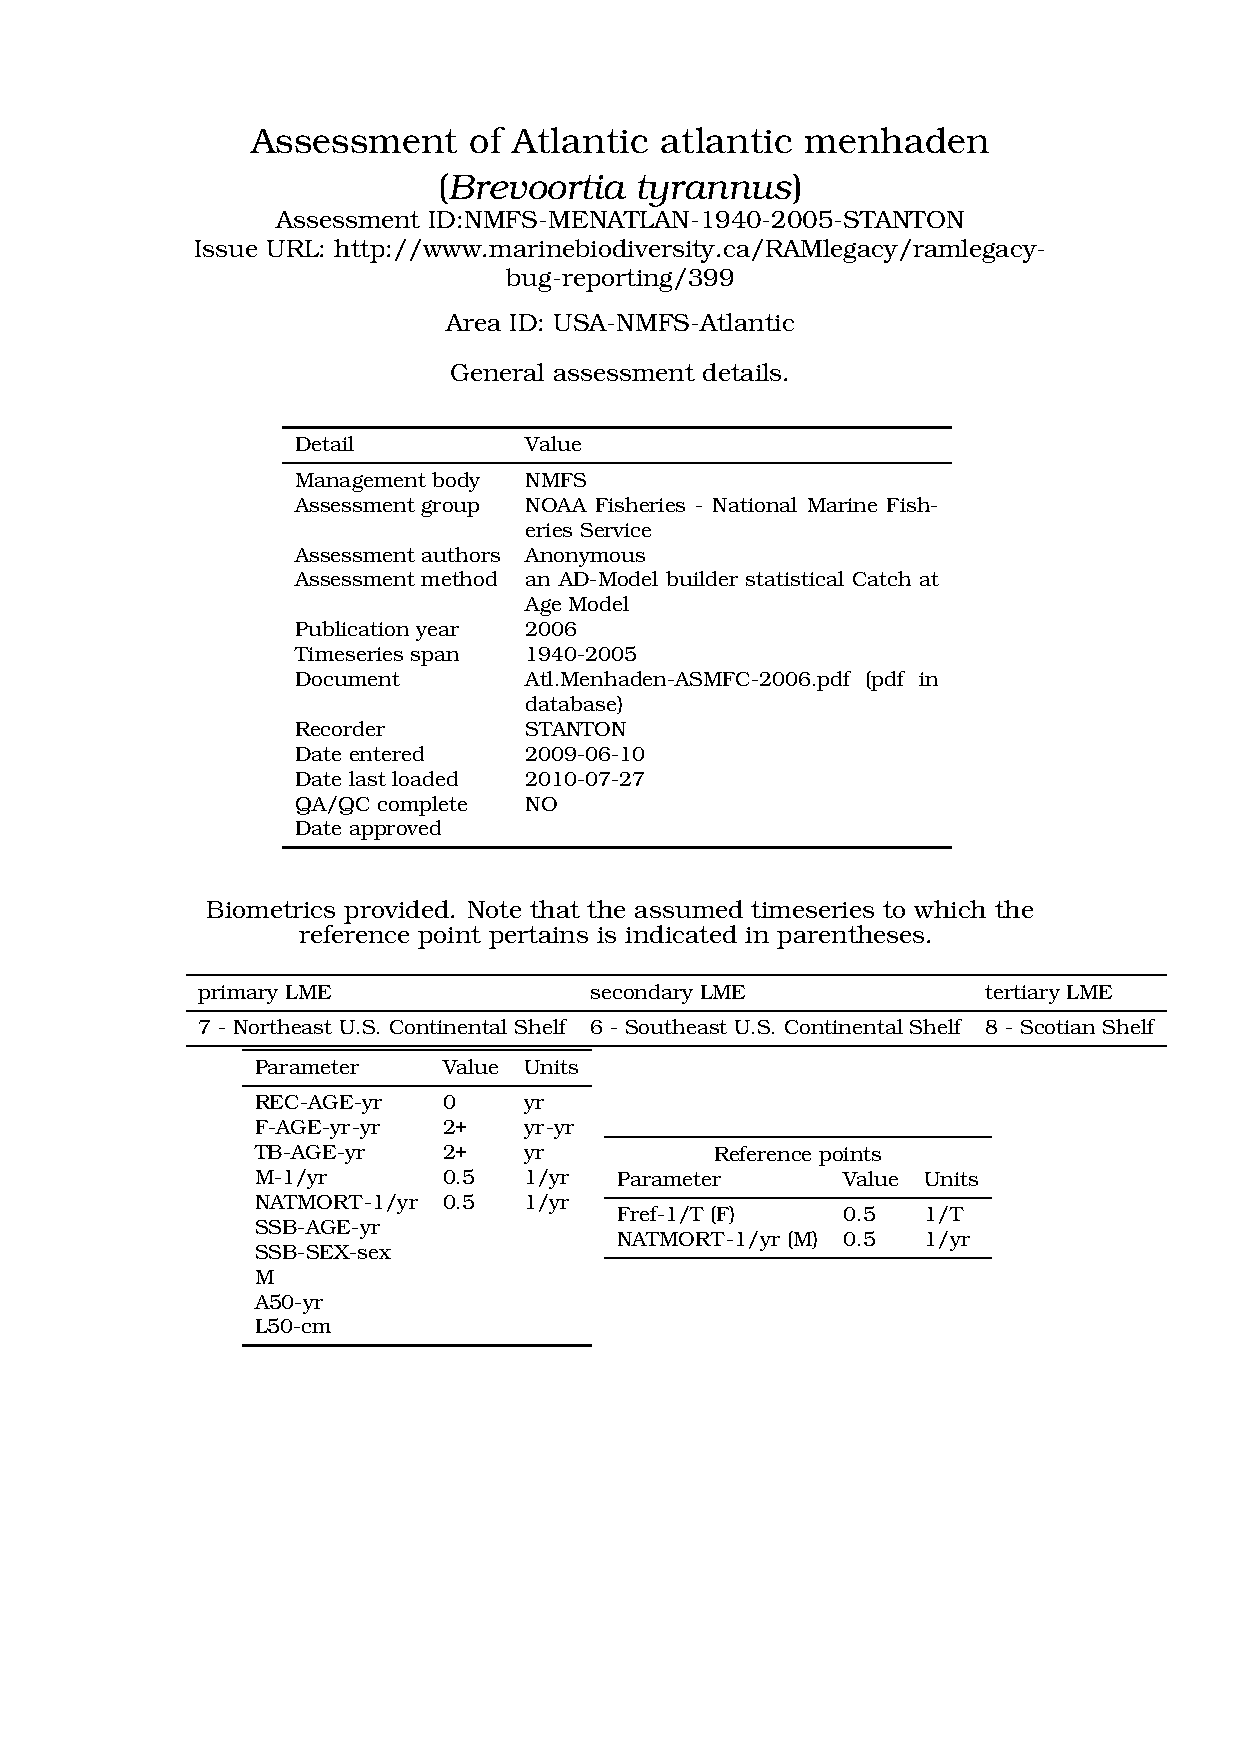
\includepdf[pagecommand={\thispagestyle{plain}}, pages={1,2}]{../../../tex/NMFS-MENATLAN-1940-2005-STANTON.pdf}
\index{Herring}\index{Clupea harengus}\index{Clupeidae!Clupea harengus}
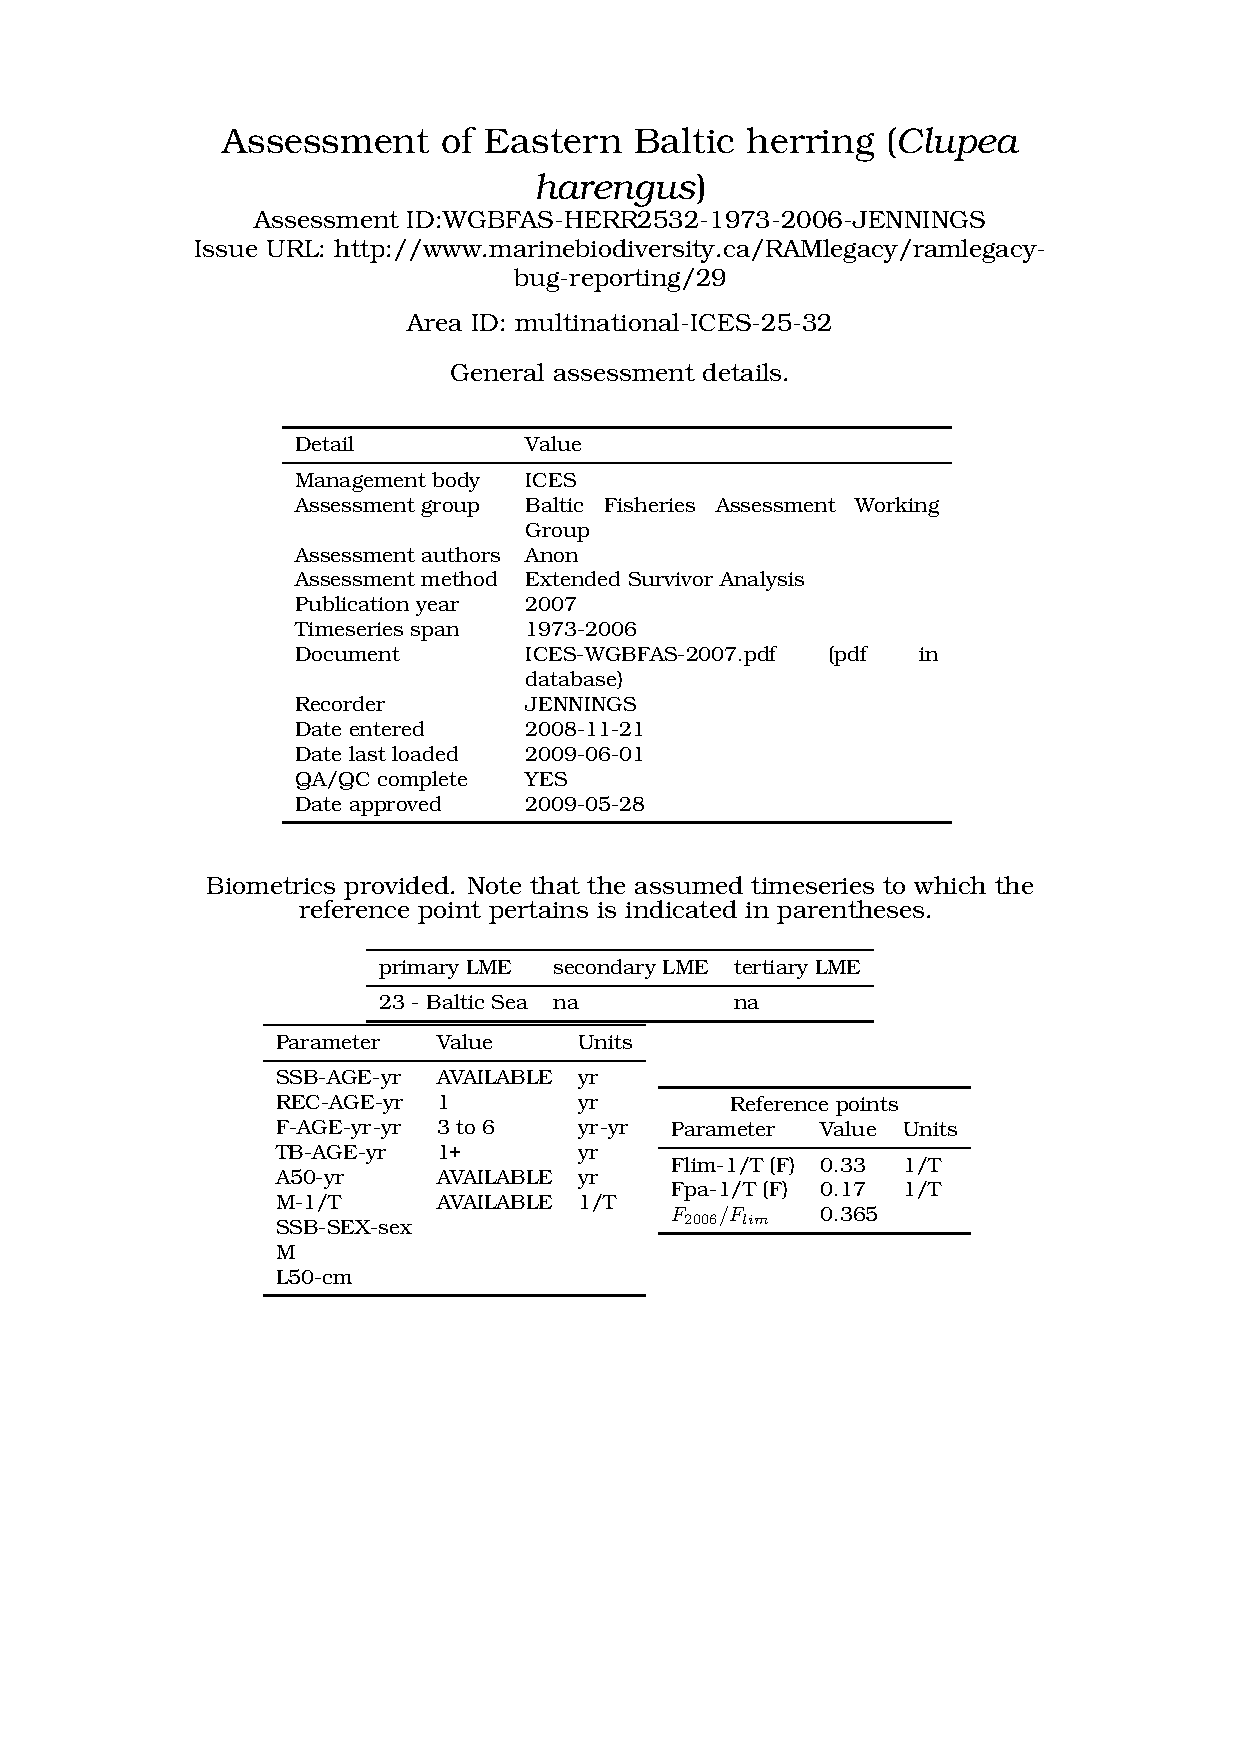
\includepdf[pagecommand={\thispagestyle{plain}}, pages={1,2}]{../../../tex/WGBFAS-HERR2532-1973-2006-JENNINGS.pdf}
\index{Herring}\index{Clupea harengus}\index{Clupeidae!Clupea harengus}
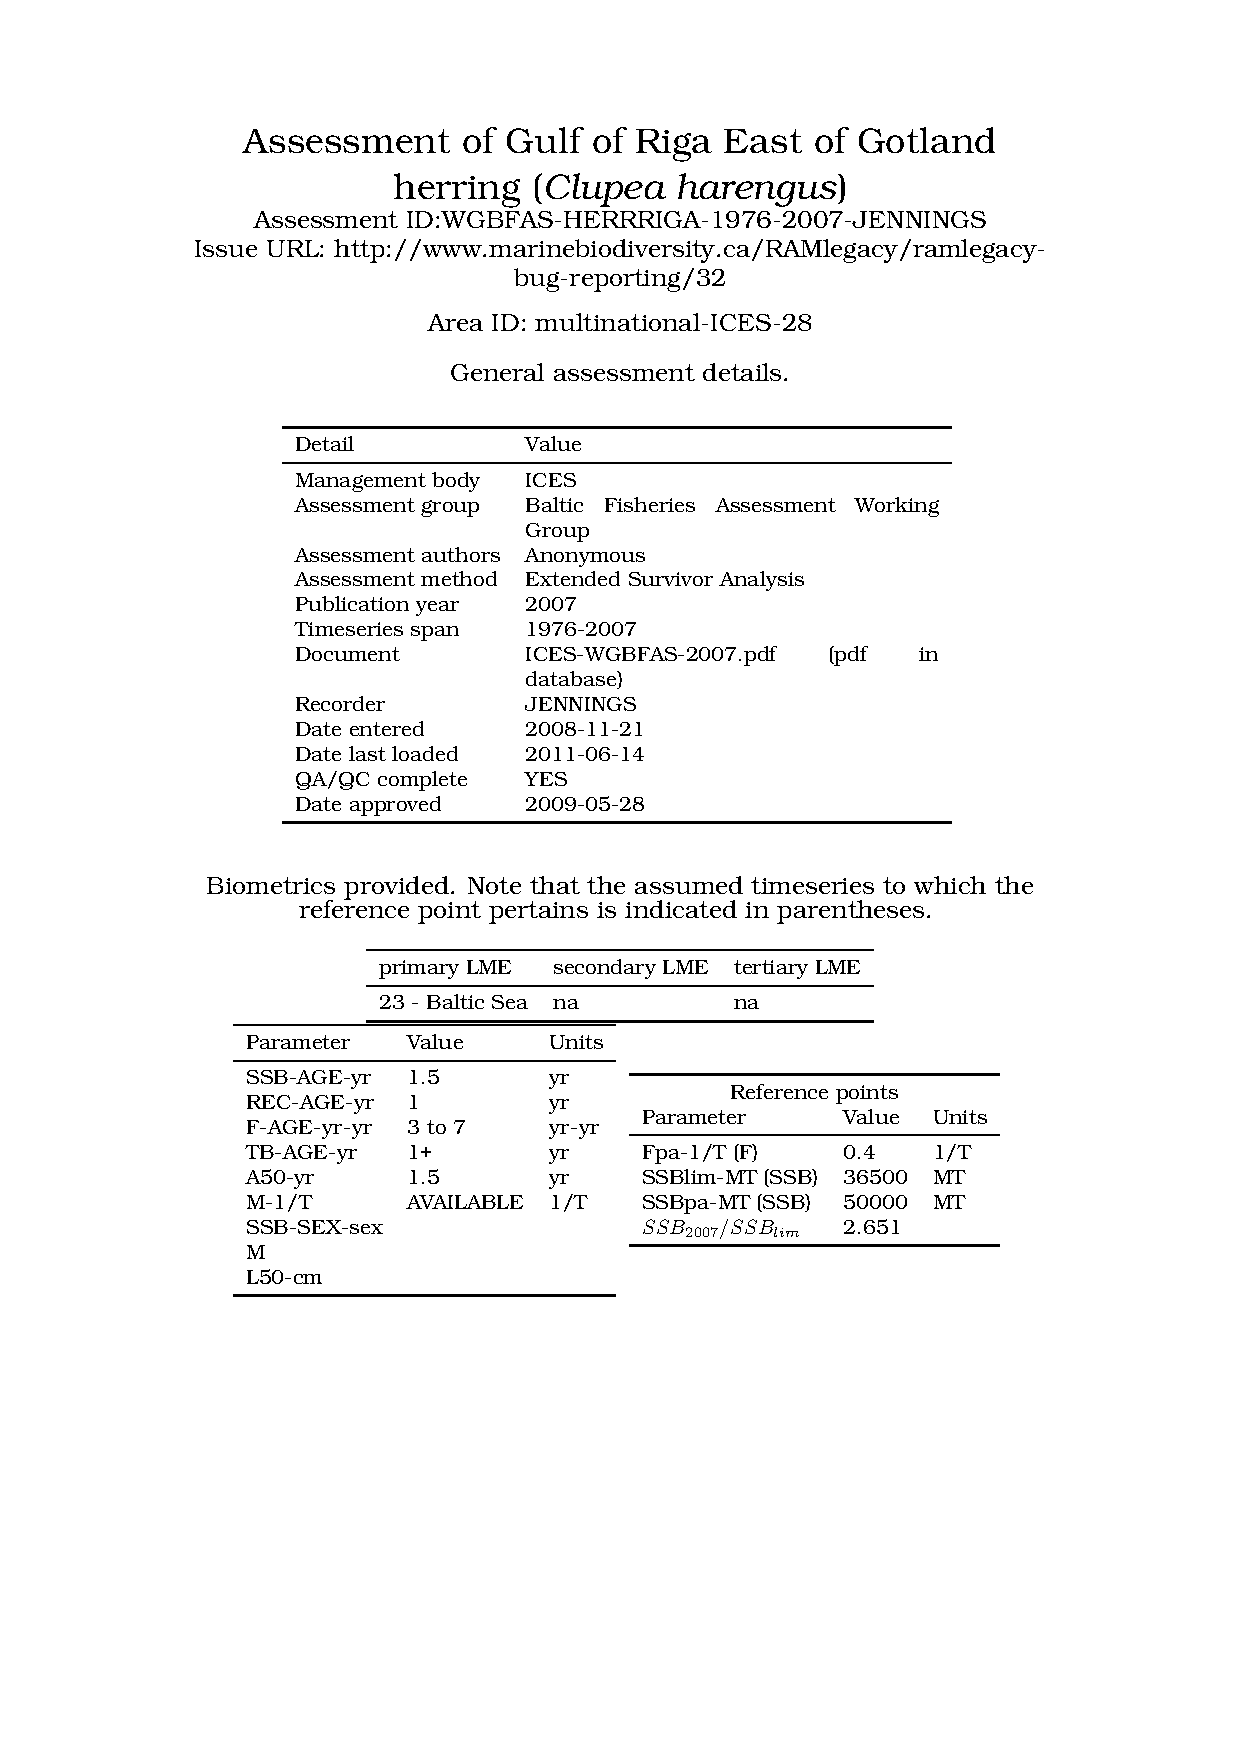
\includepdf[pagecommand={\thispagestyle{plain}}, pages={1,2}]{../../../tex/WGBFAS-HERRRIGA-1976-2007-JENNINGS.pdf}
\index{Herring}\index{Clupea harengus}\index{Clupeidae!Clupea harengus}
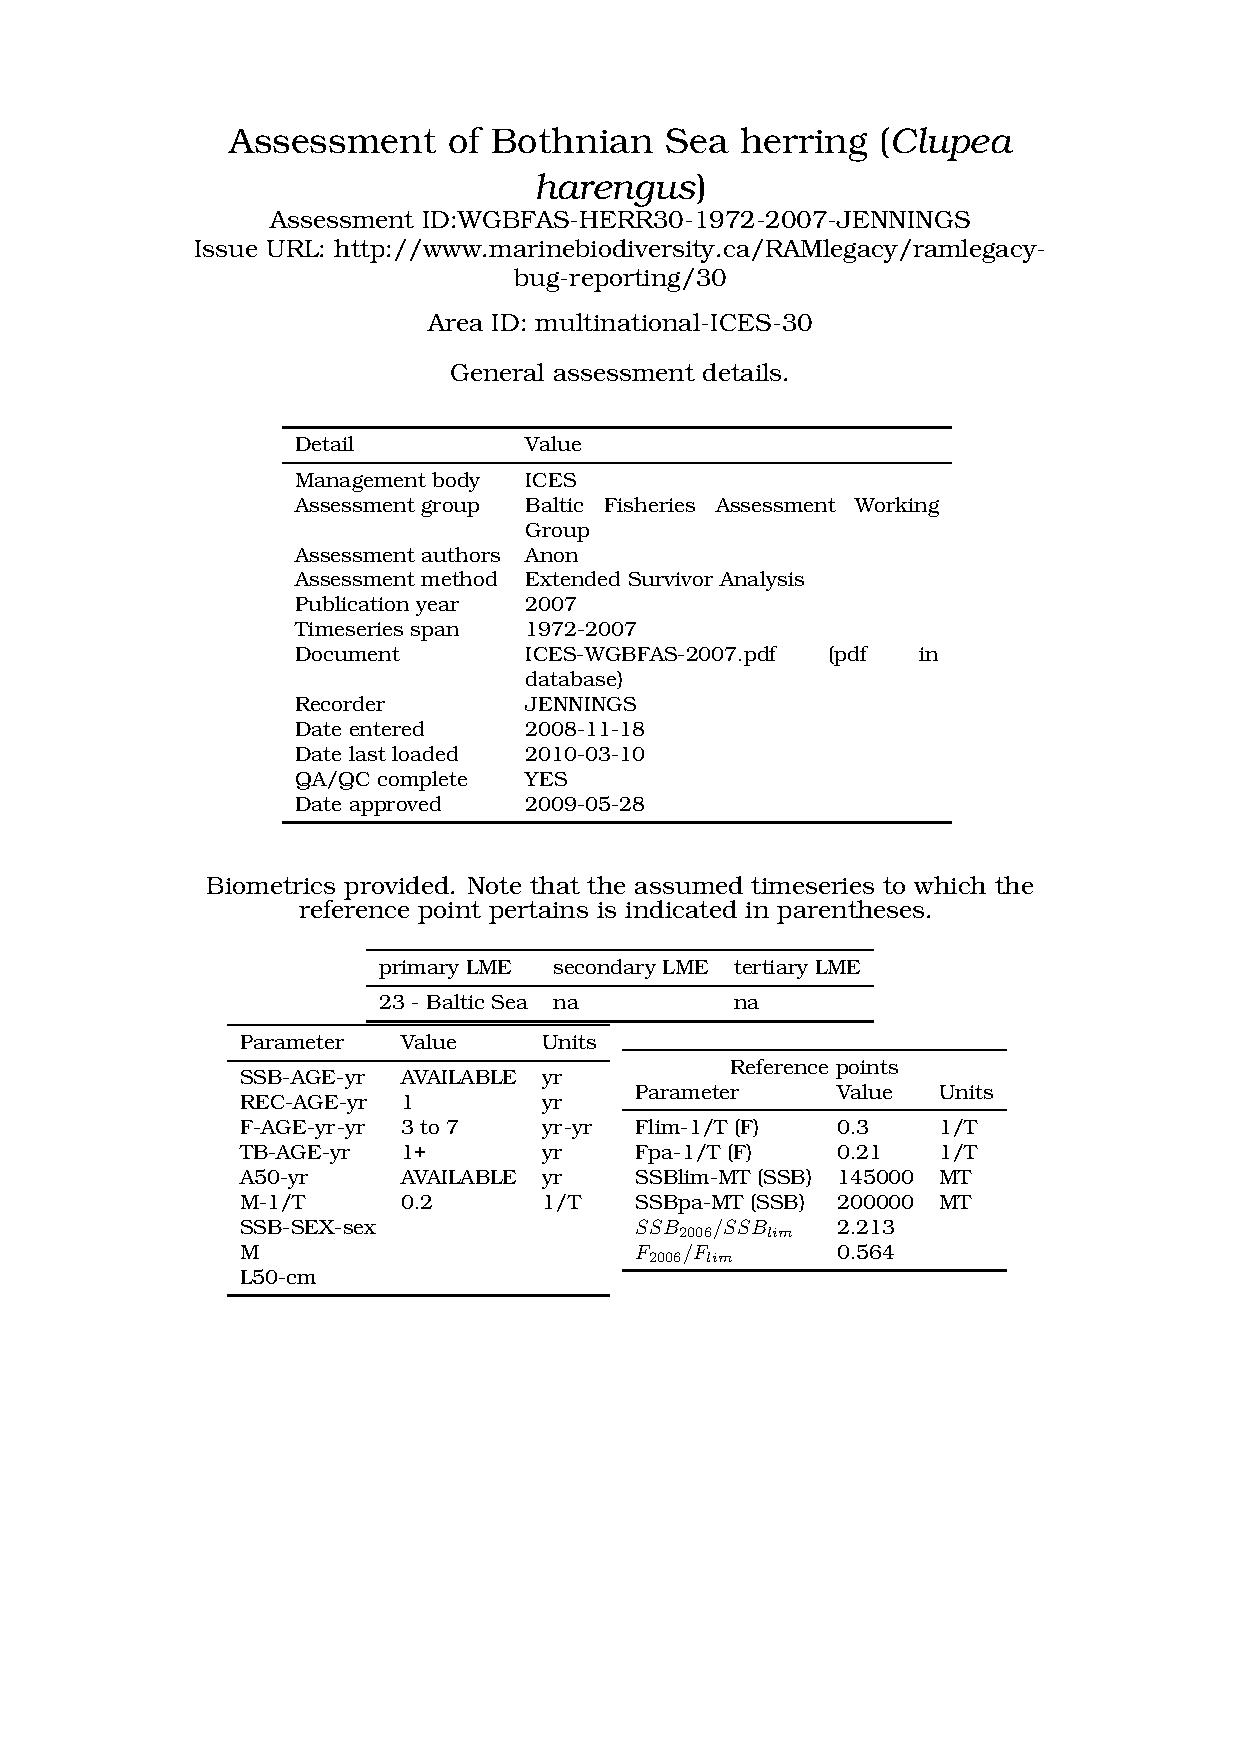
\includepdf[pagecommand={\thispagestyle{plain}}, pages={1,2}]{../../../tex/WGBFAS-HERR30-1972-2007-JENNINGS.pdf}
\index{Herring}\index{Clupea harengus}\index{Clupeidae!Clupea harengus}
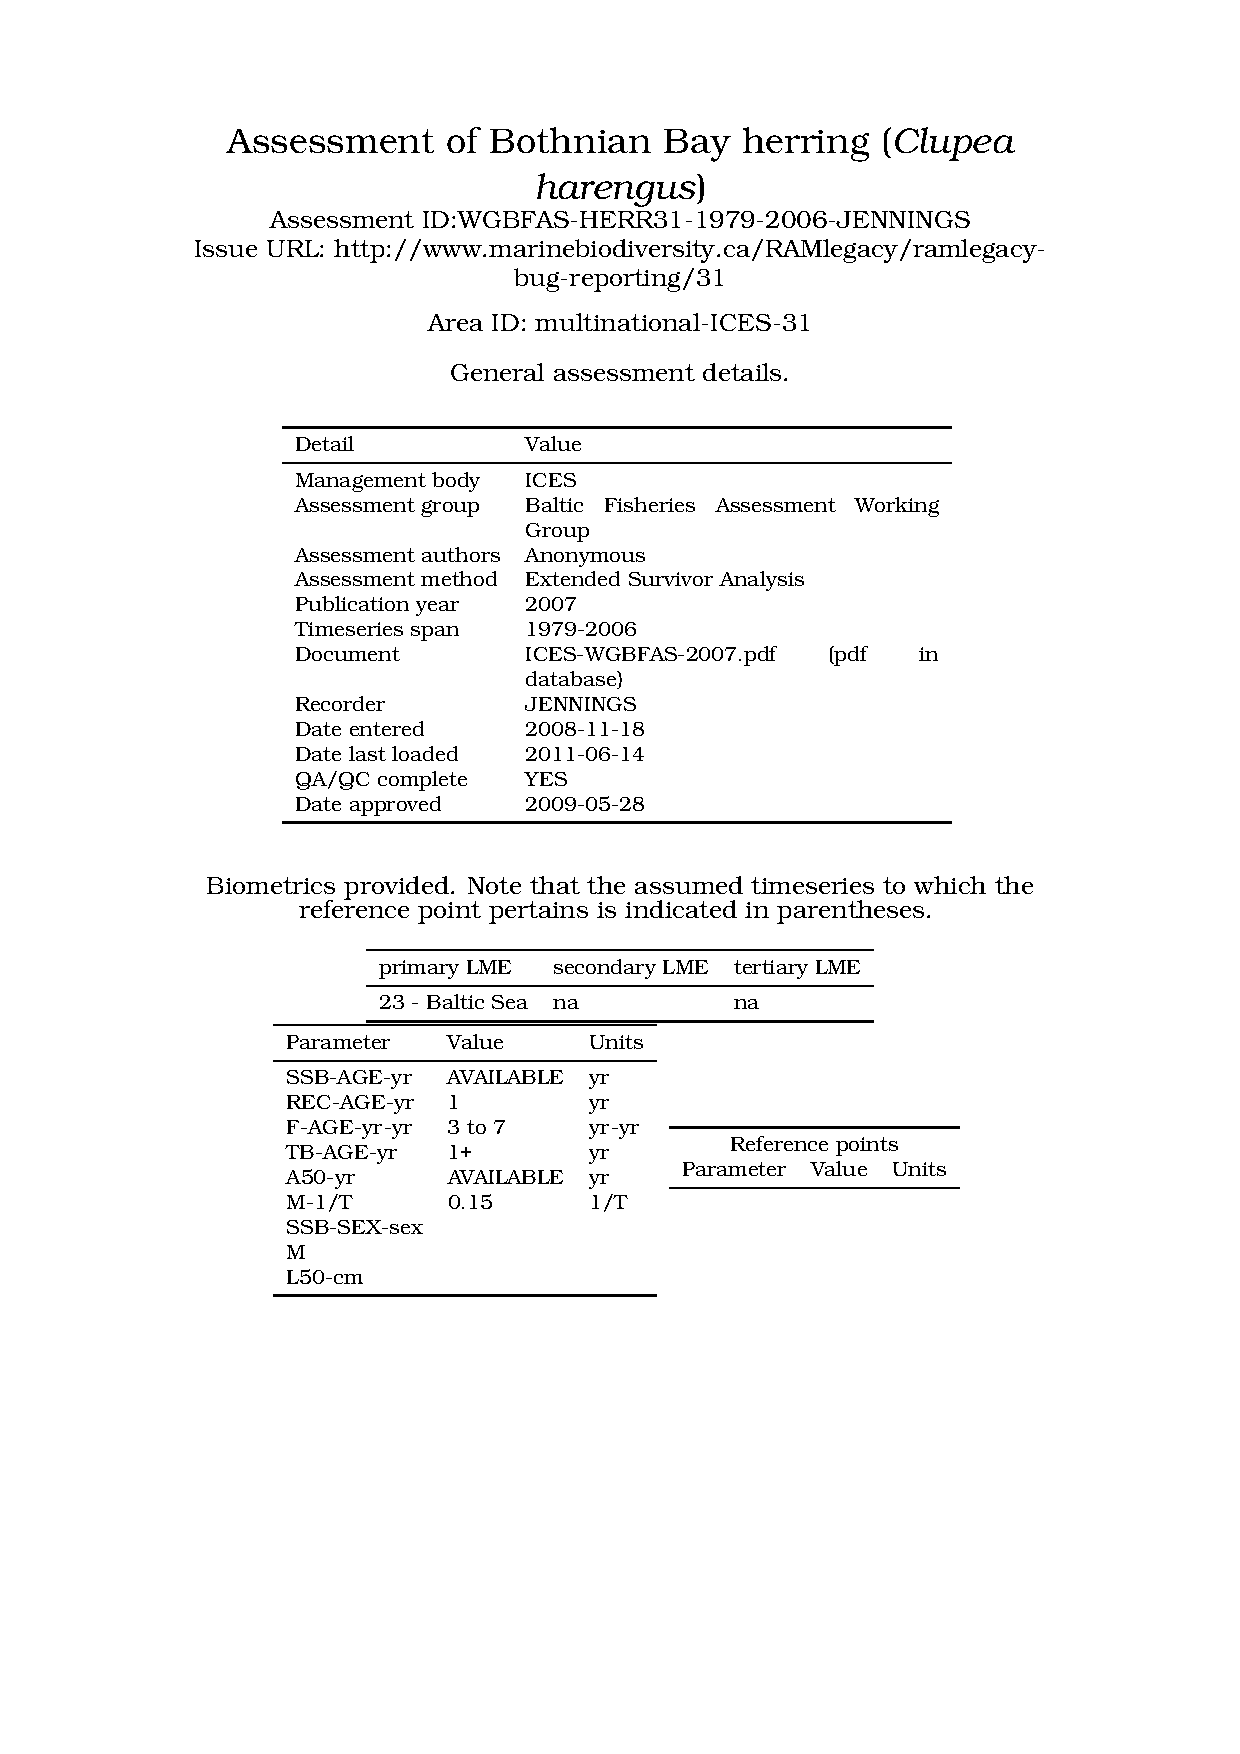
\includepdf[pagecommand={\thispagestyle{plain}}, pages={1,2}]{../../../tex/WGBFAS-HERR31-1979-2006-JENNINGS.pdf}
\index{Herring}\index{Clupea harengus}\index{Clupeidae!Clupea harengus}
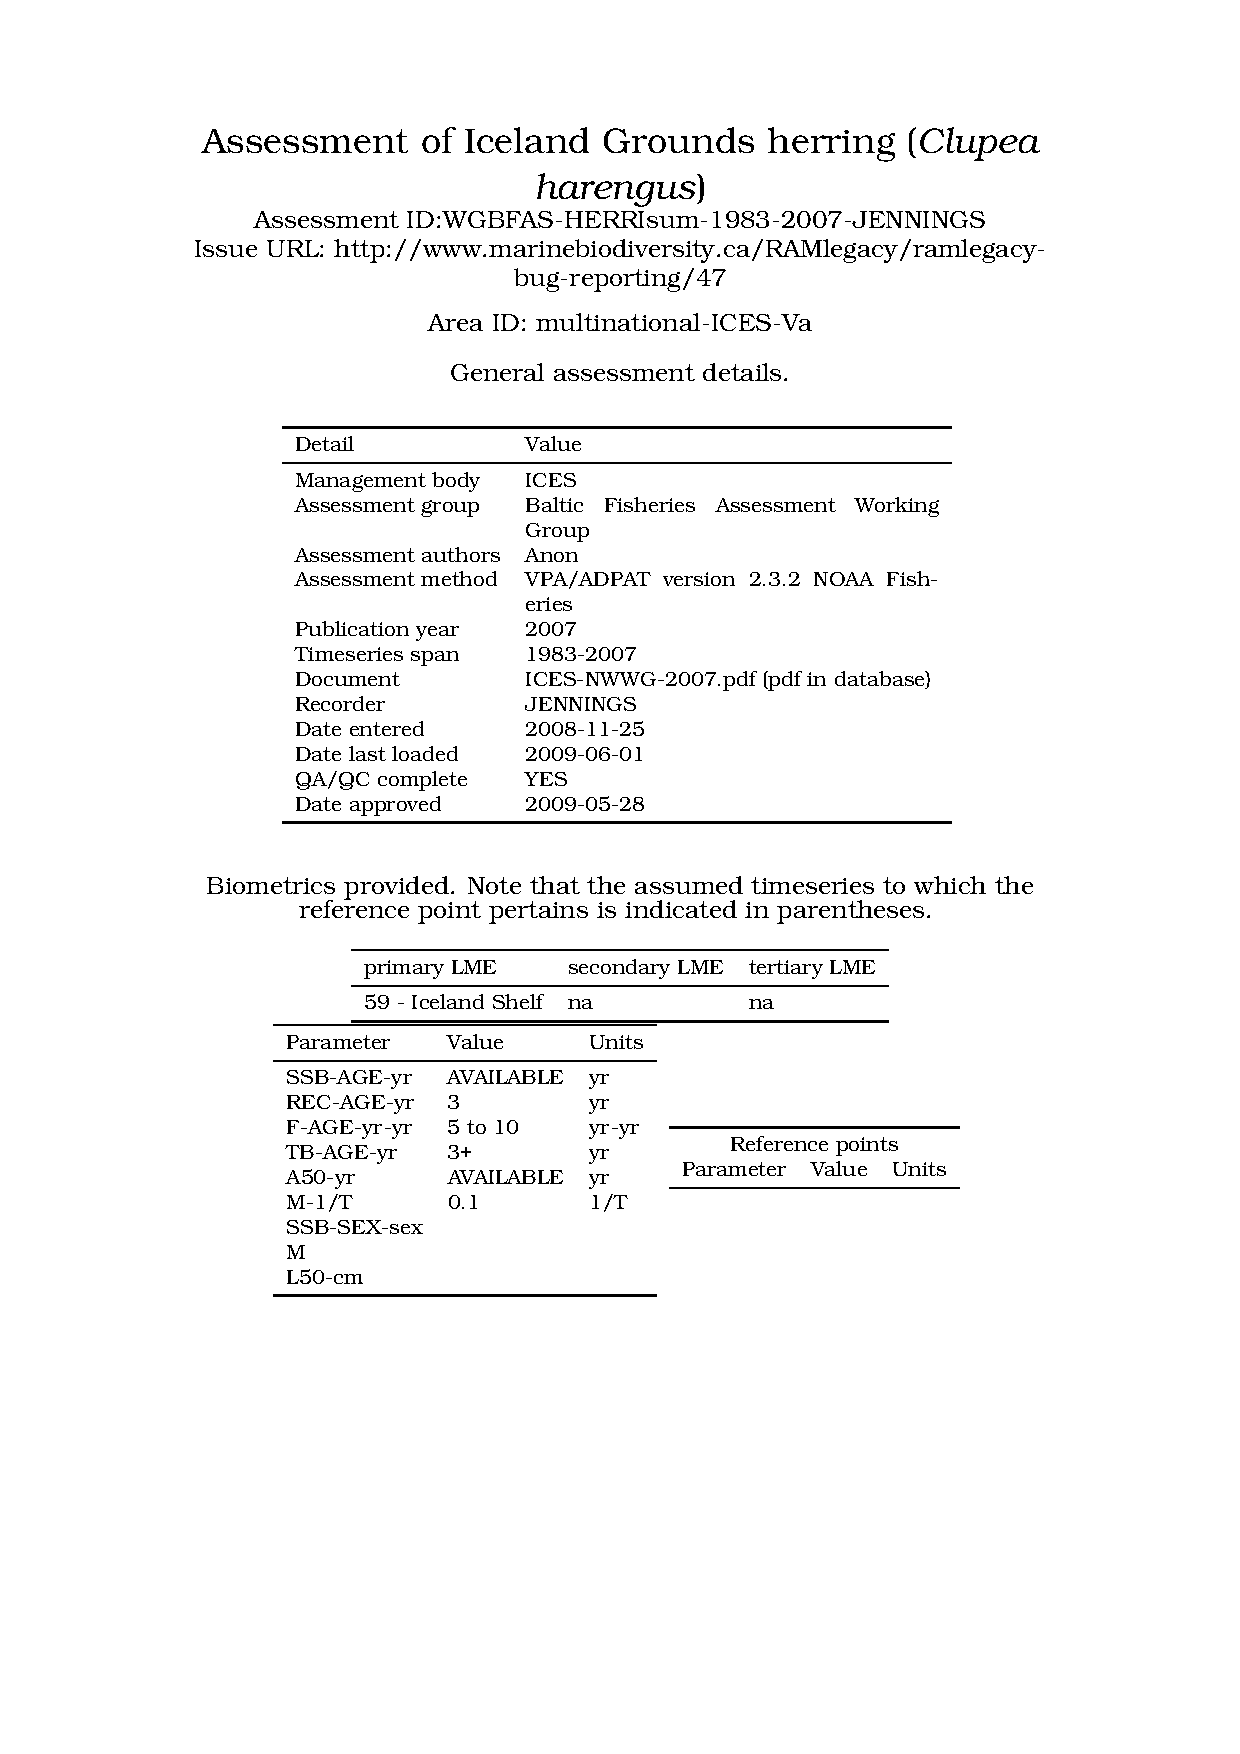
\includepdf[pagecommand={\thispagestyle{plain}}, pages={1,2}]{../../../tex/WGBFAS-HERRIsum-1983-2007-JENNINGS.pdf}
\index{Herring}\index{Clupea harengus}\index{Clupeidae!Clupea harengus}
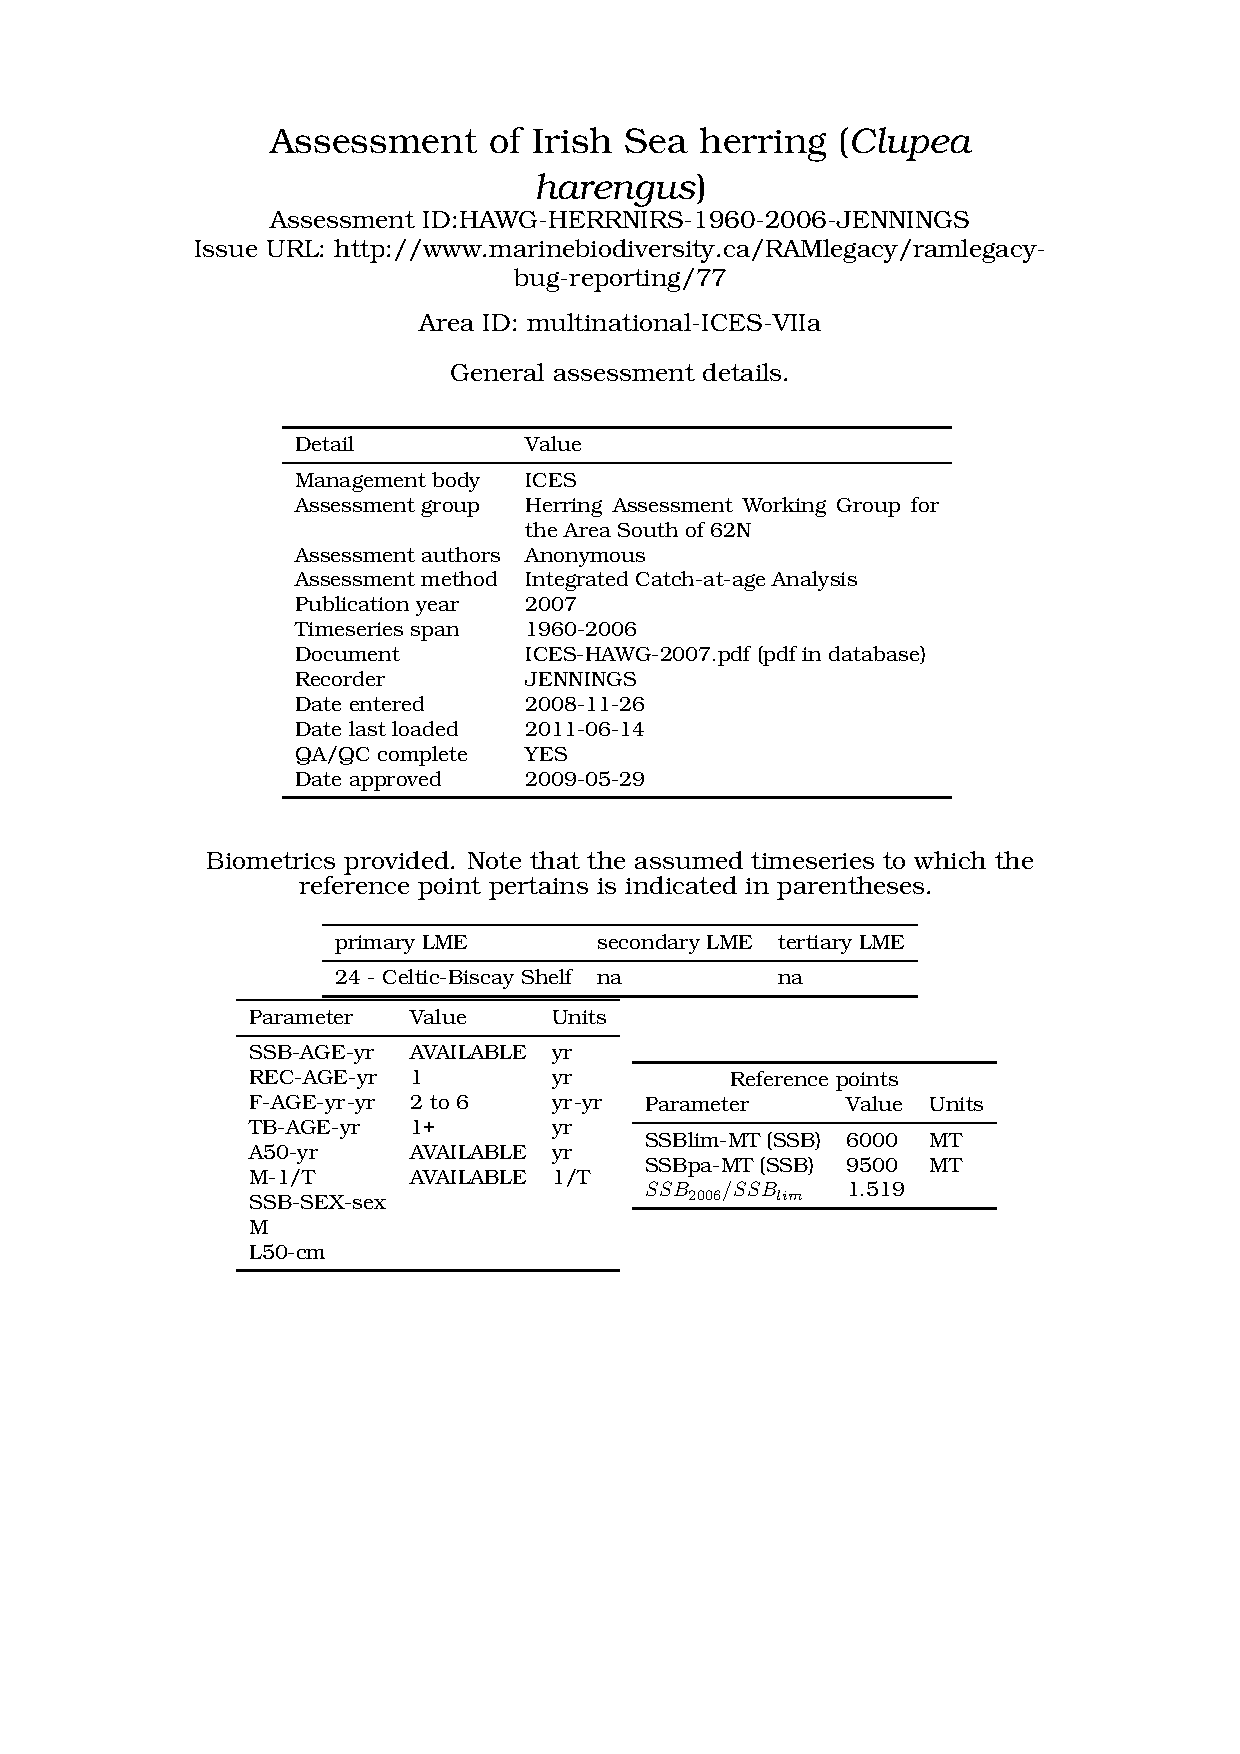
\includepdf[pagecommand={\thispagestyle{plain}}, pages={1,2}]{../../../tex/HAWG-HERRNIRS-1960-2006-JENNINGS.pdf}
\index{Herring}\index{Clupea harengus}\index{Clupeidae!Clupea harengus}
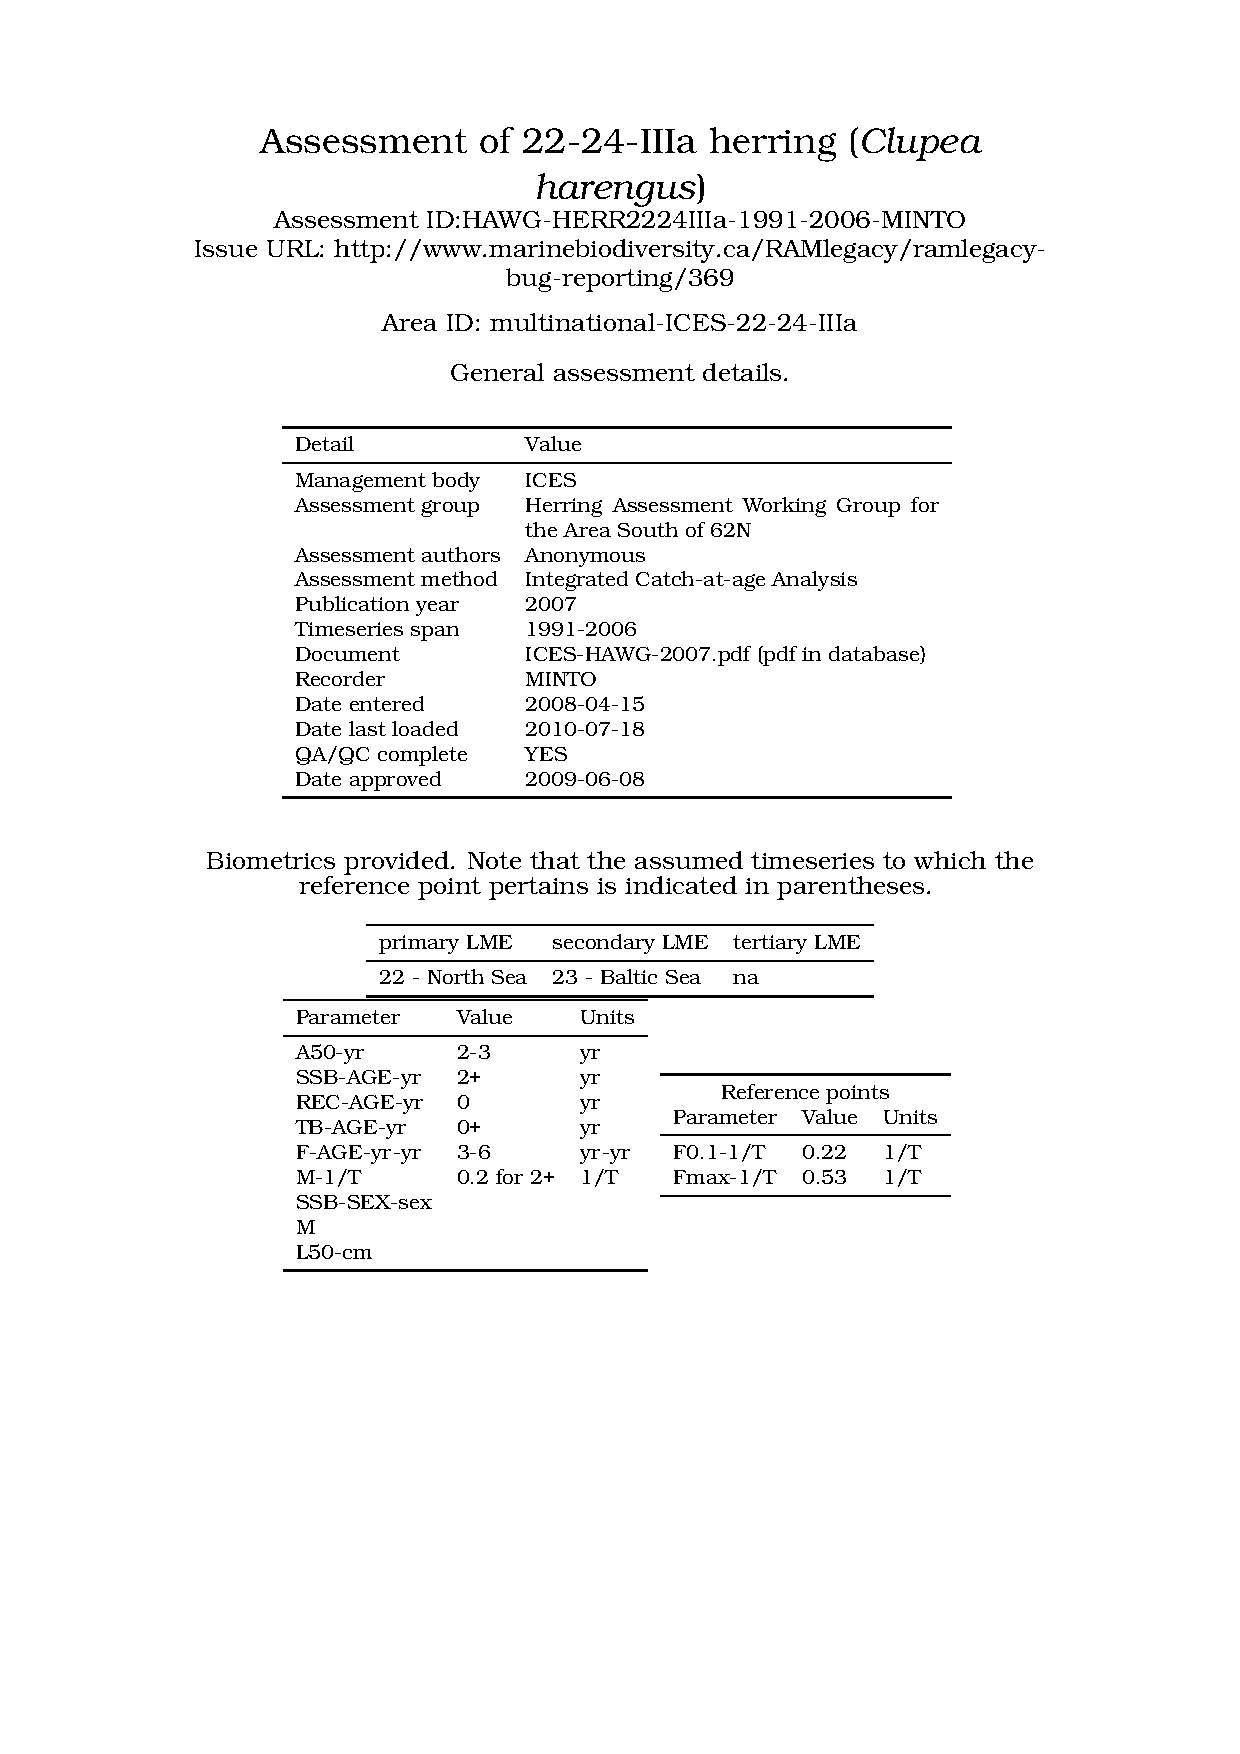
\includepdf[pagecommand={\thispagestyle{plain}}, pages={1,2}]{../../../tex/HAWG-HERR2224IIIa-1991-2006-MINTO.pdf}
\index{Herring}\index{Clupea harengus}\index{Clupeidae!Clupea harengus}
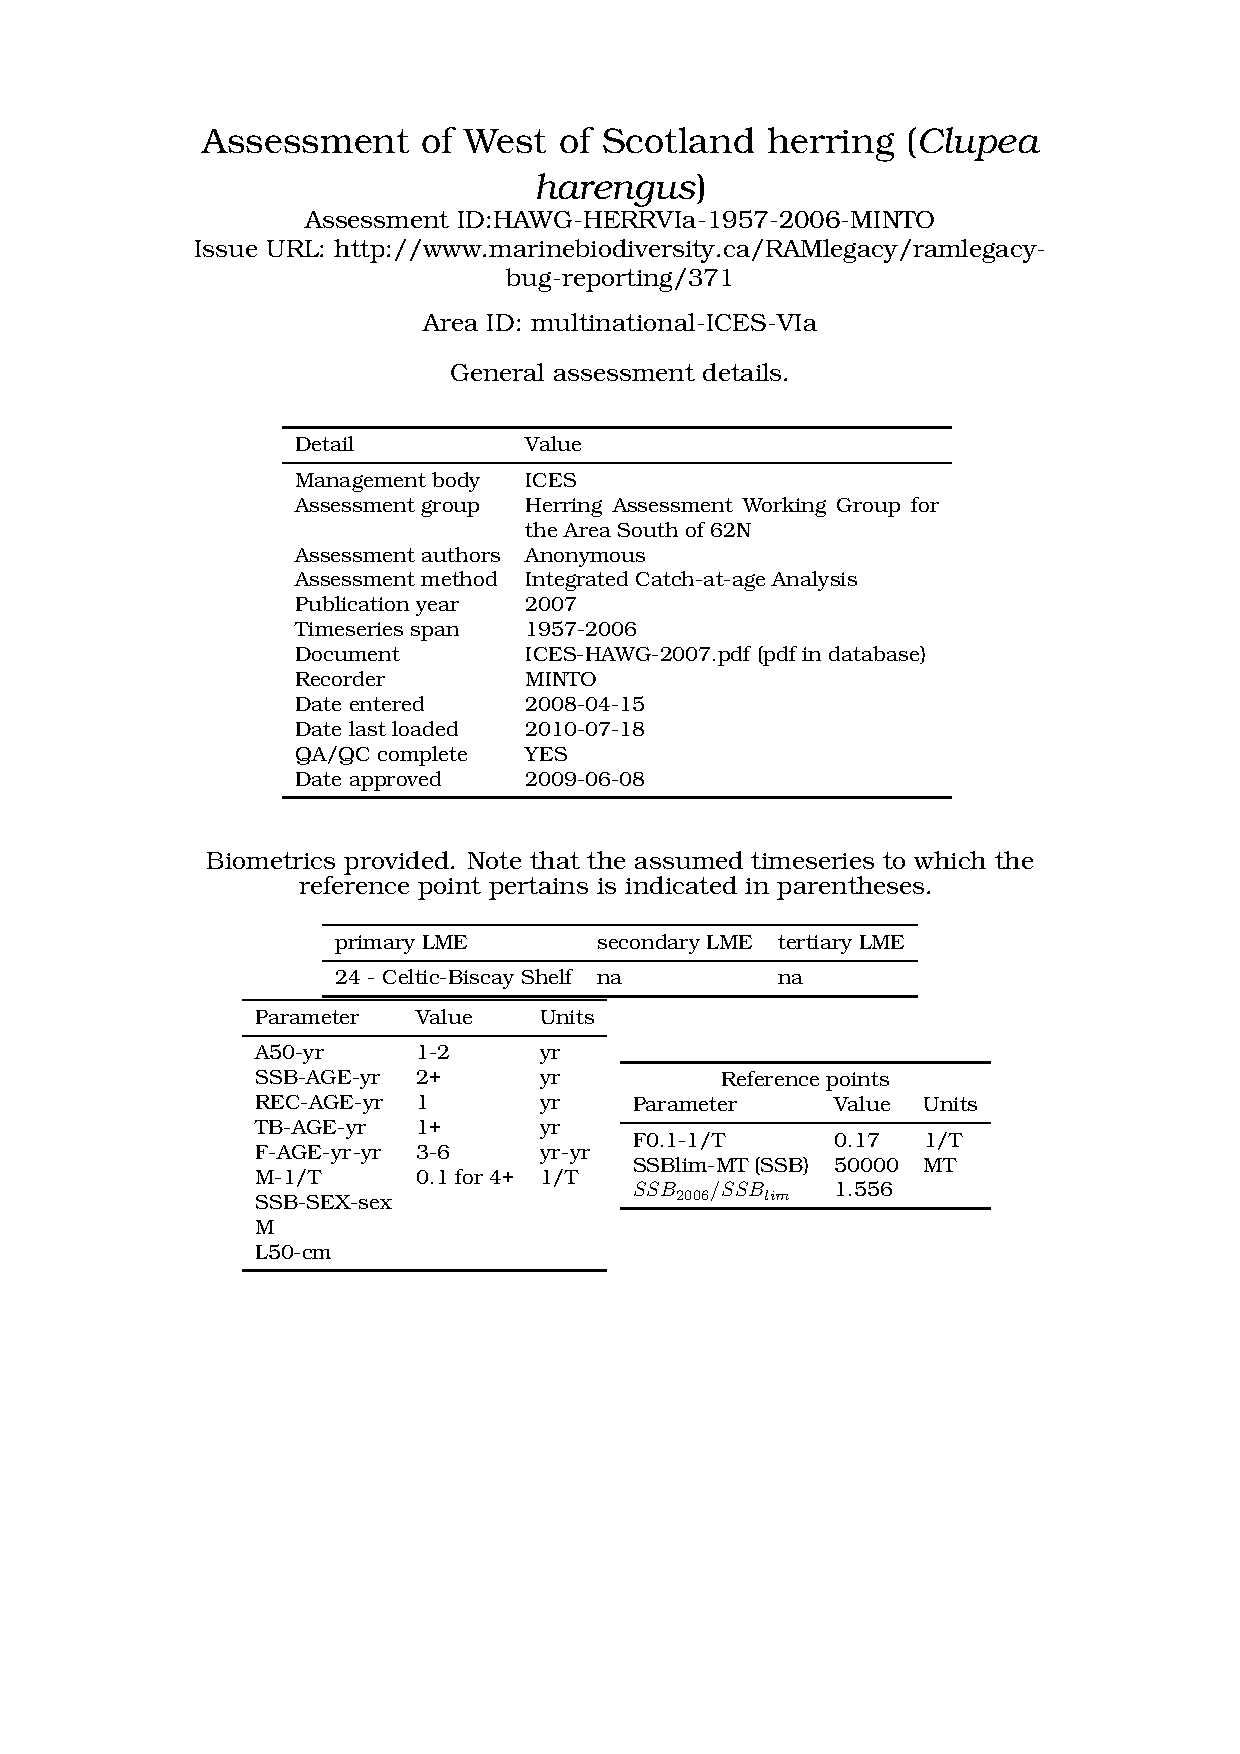
\includepdf[pagecommand={\thispagestyle{plain}}, pages={1,2}]{../../../tex/HAWG-HERRVIa-1957-2006-MINTO.pdf}
\index{Herring}\index{Clupea harengus}\index{Clupeidae!Clupea harengus}
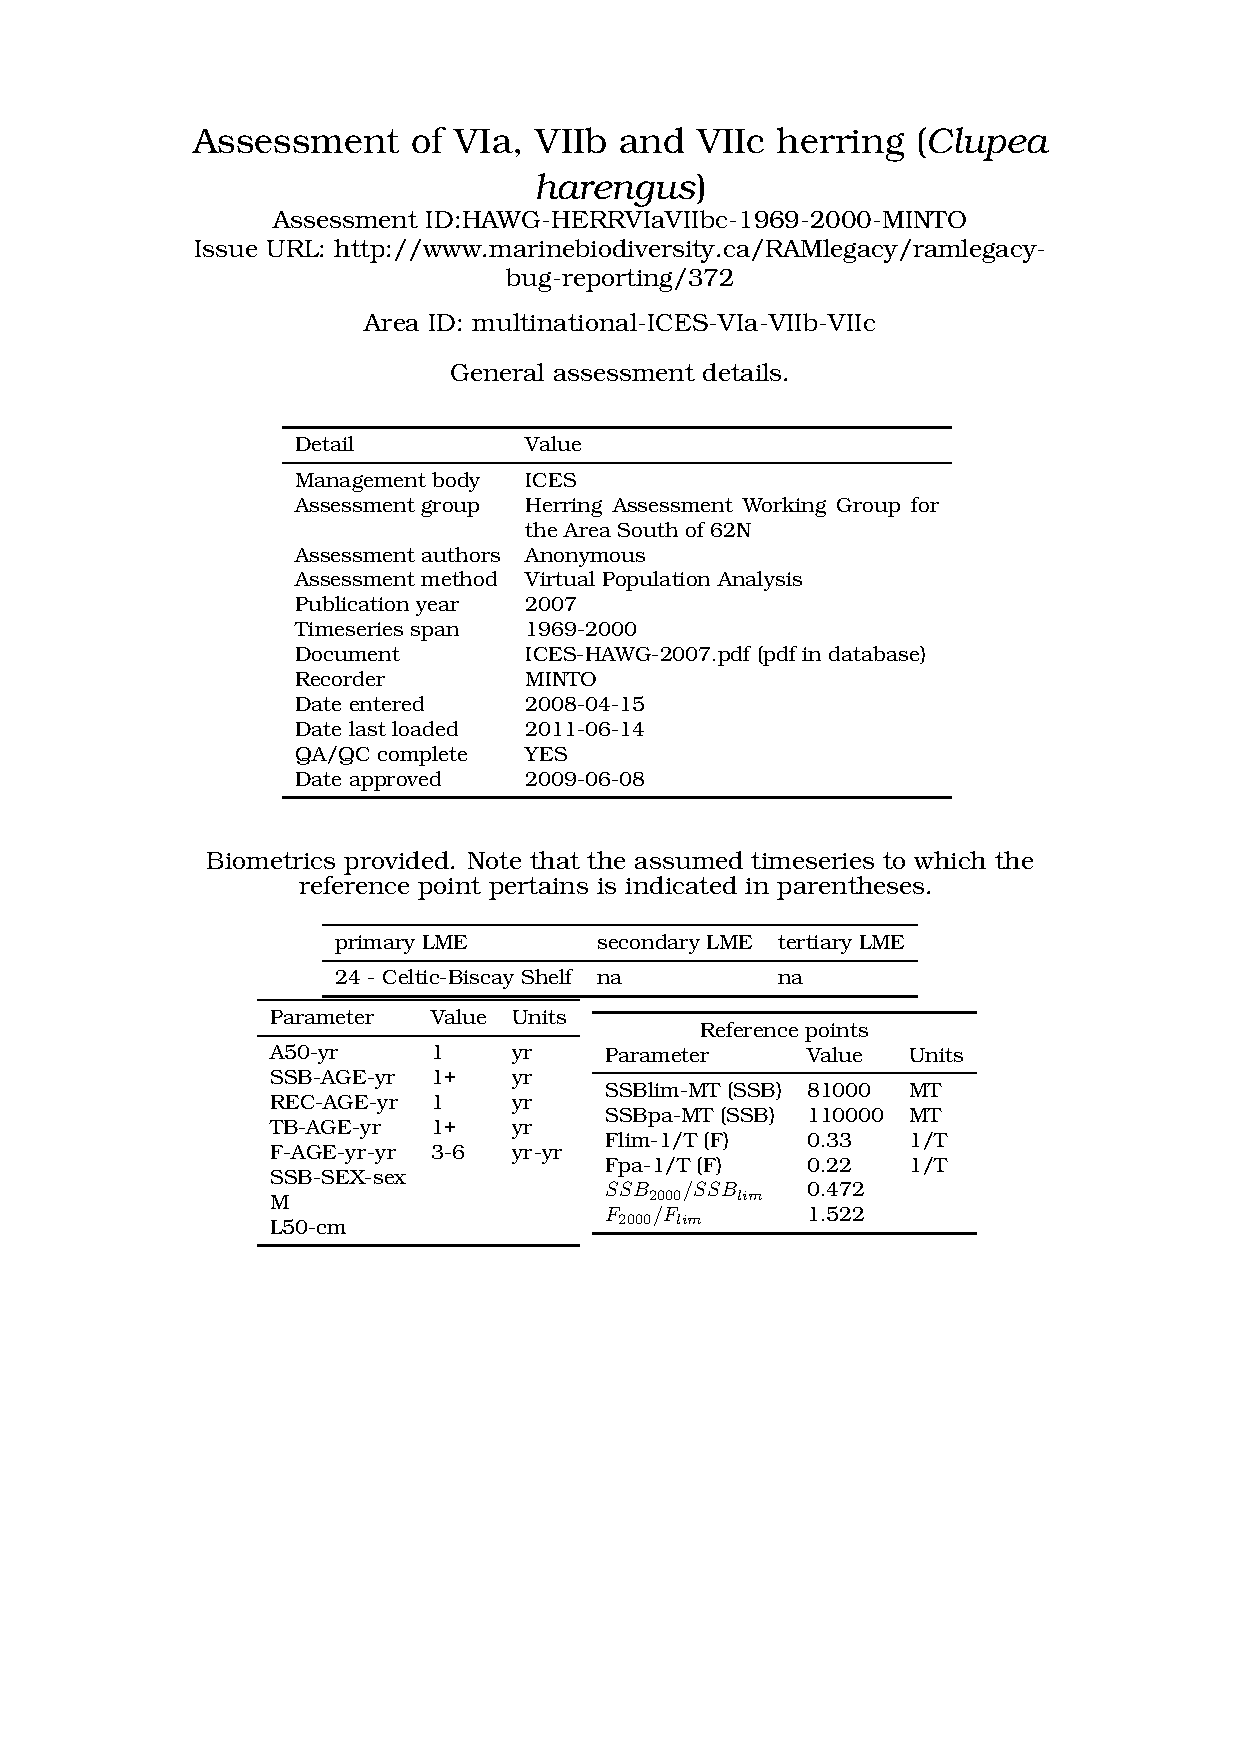
\includepdf[pagecommand={\thispagestyle{plain}}, pages={1,2}]{../../../tex/HAWG-HERRVIaVIIbc-1969-2000-MINTO.pdf}
\index{Herring}\index{Clupea harengus}\index{Clupeidae!Clupea harengus}
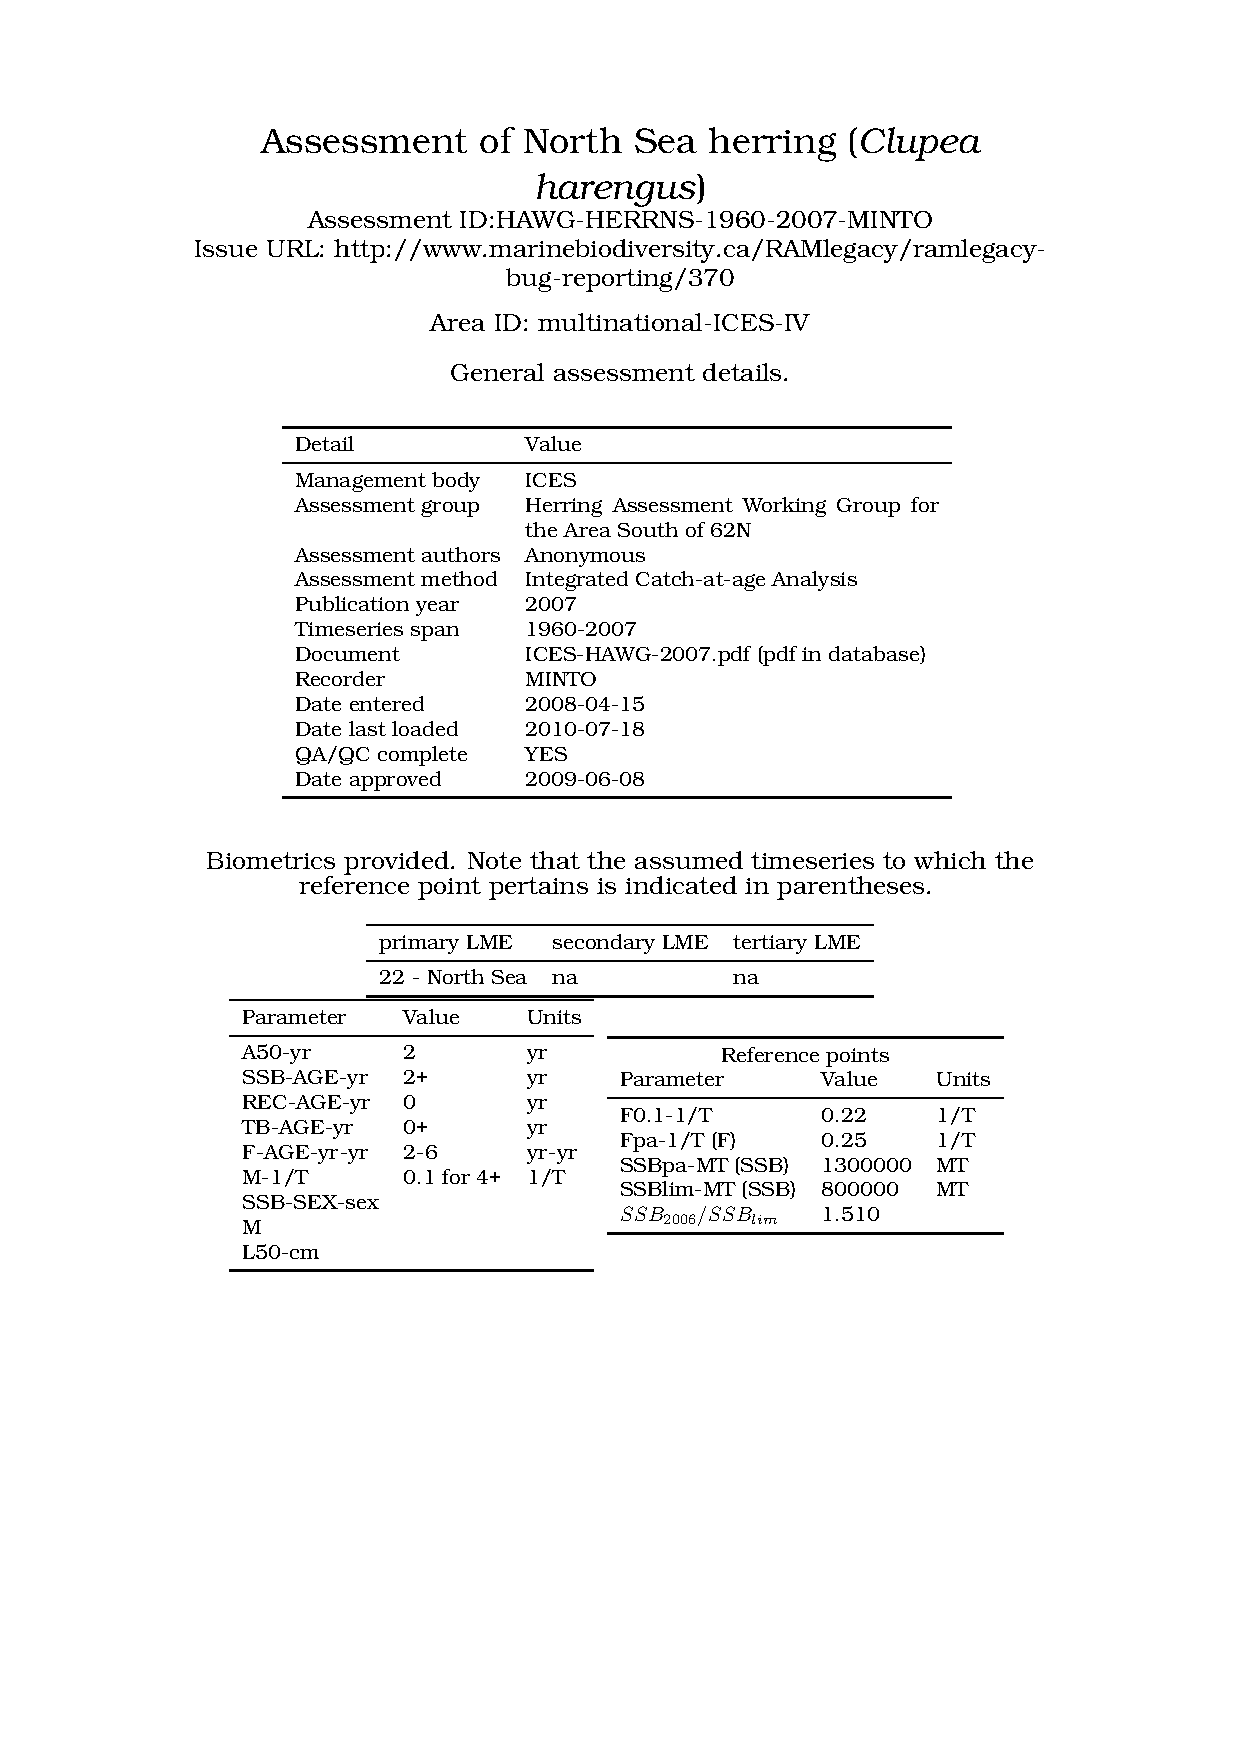
\includepdf[pagecommand={\thispagestyle{plain}}, pages={1,2}]{../../../tex/HAWG-HERRNS-1960-2007-MINTO.pdf}
\index{Herring}\index{Clupea harengus}\index{Clupeidae!Clupea harengus}
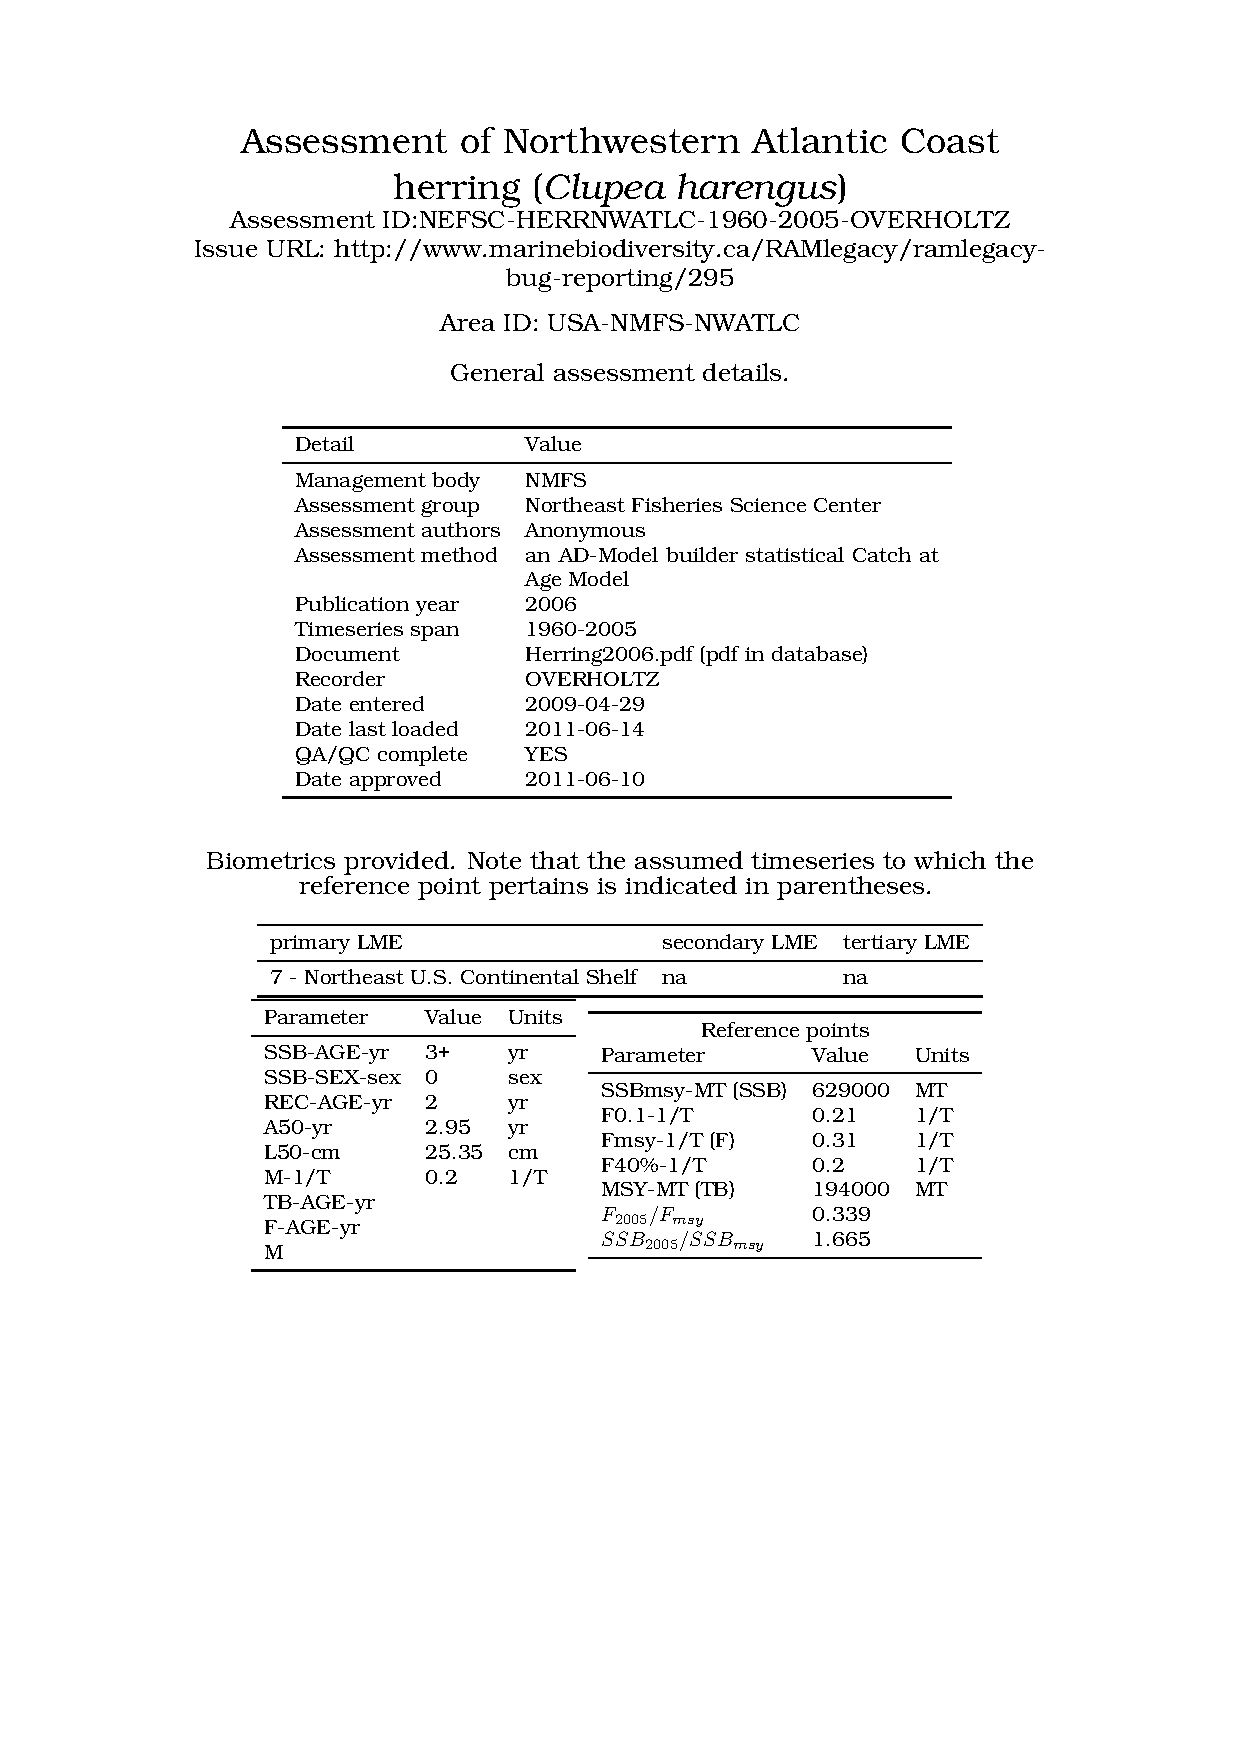
\includepdf[pagecommand={\thispagestyle{plain}}, pages={1,2}]{../../../tex/NEFSC-HERRNWATLC-1960-2005-OVERHOLTZ.pdf}
\index{Herring}\index{Clupea harengus}\index{Clupeidae!Clupea harengus}
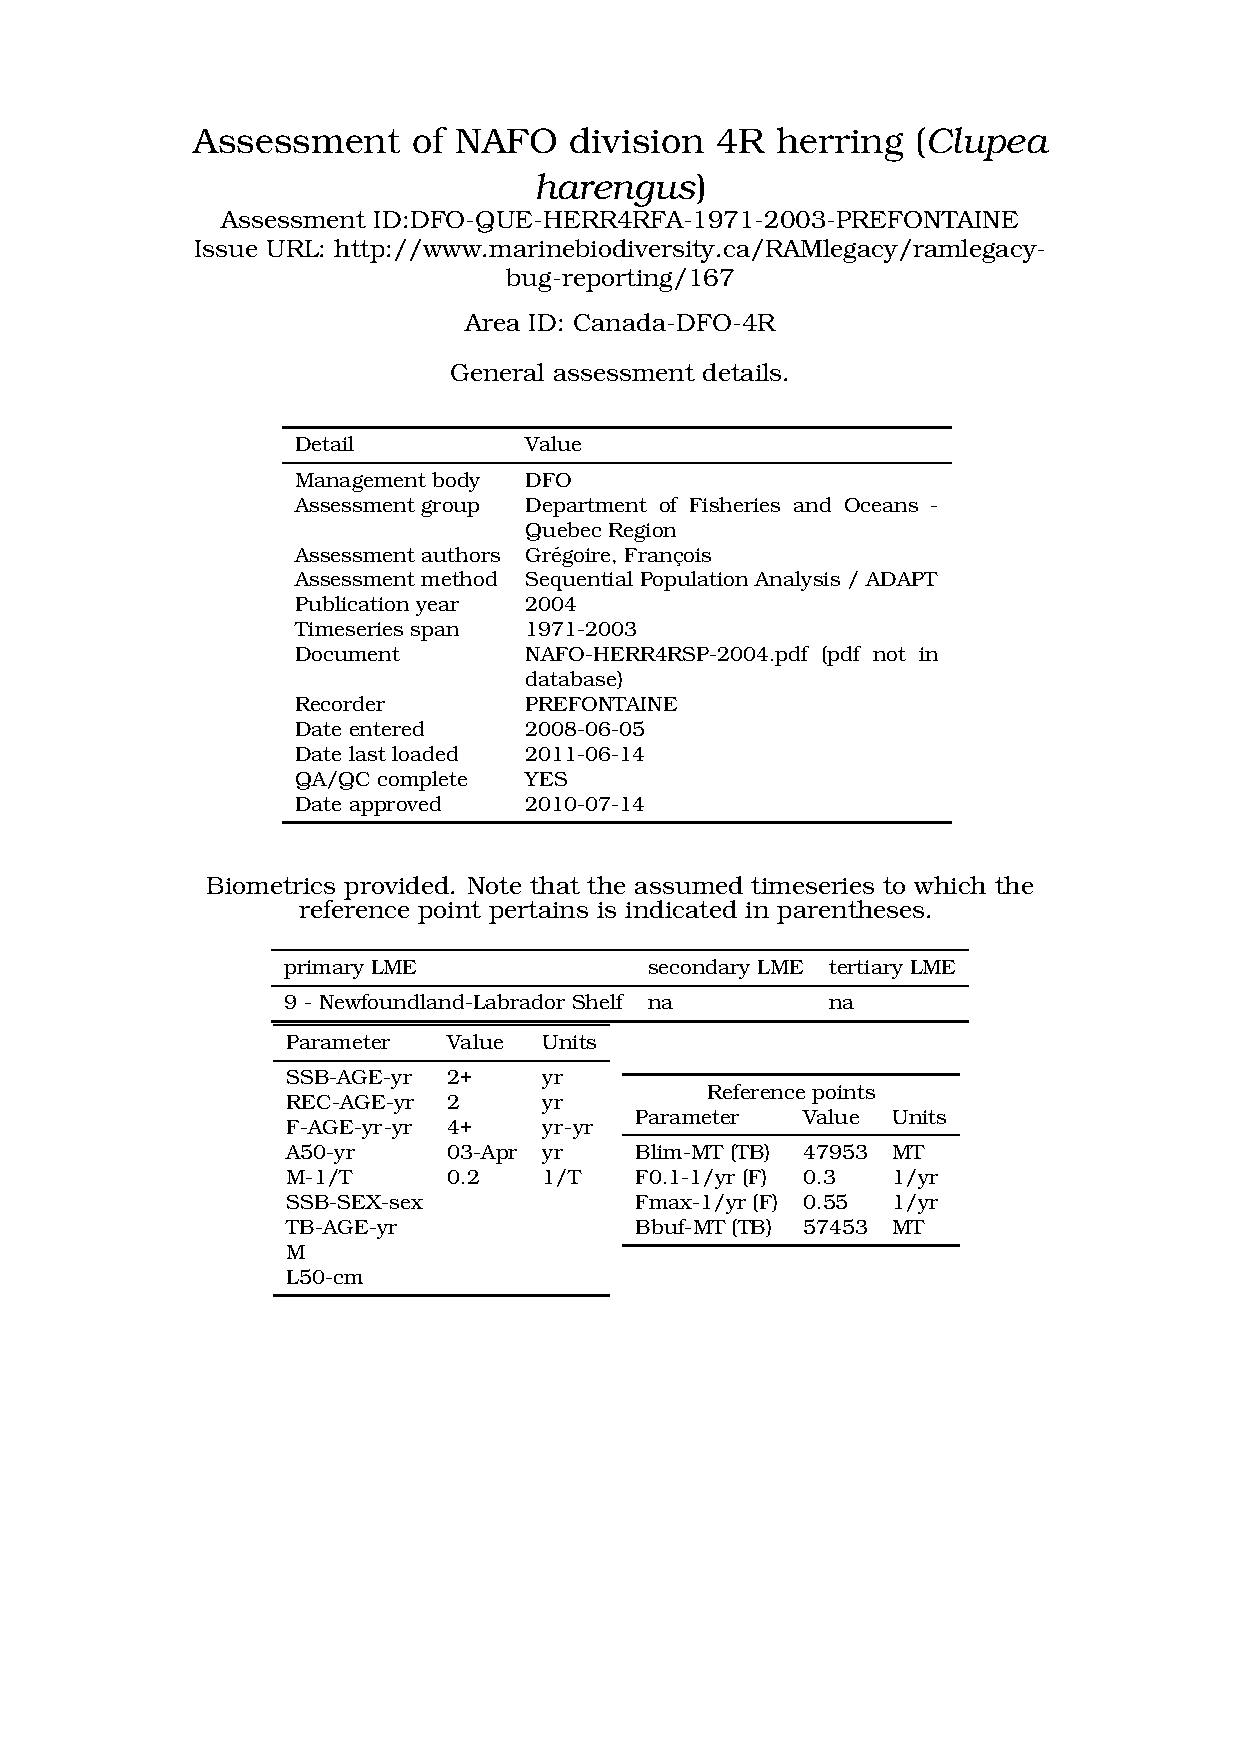
\includepdf[pagecommand={\thispagestyle{plain}}, pages={1,2}]{../../../tex/DFO-QUE-HERR4RFA-1971-2003-PREFONTAINE.pdf}
\index{Herring}\index{Clupea harengus}\index{Clupeidae!Clupea harengus}
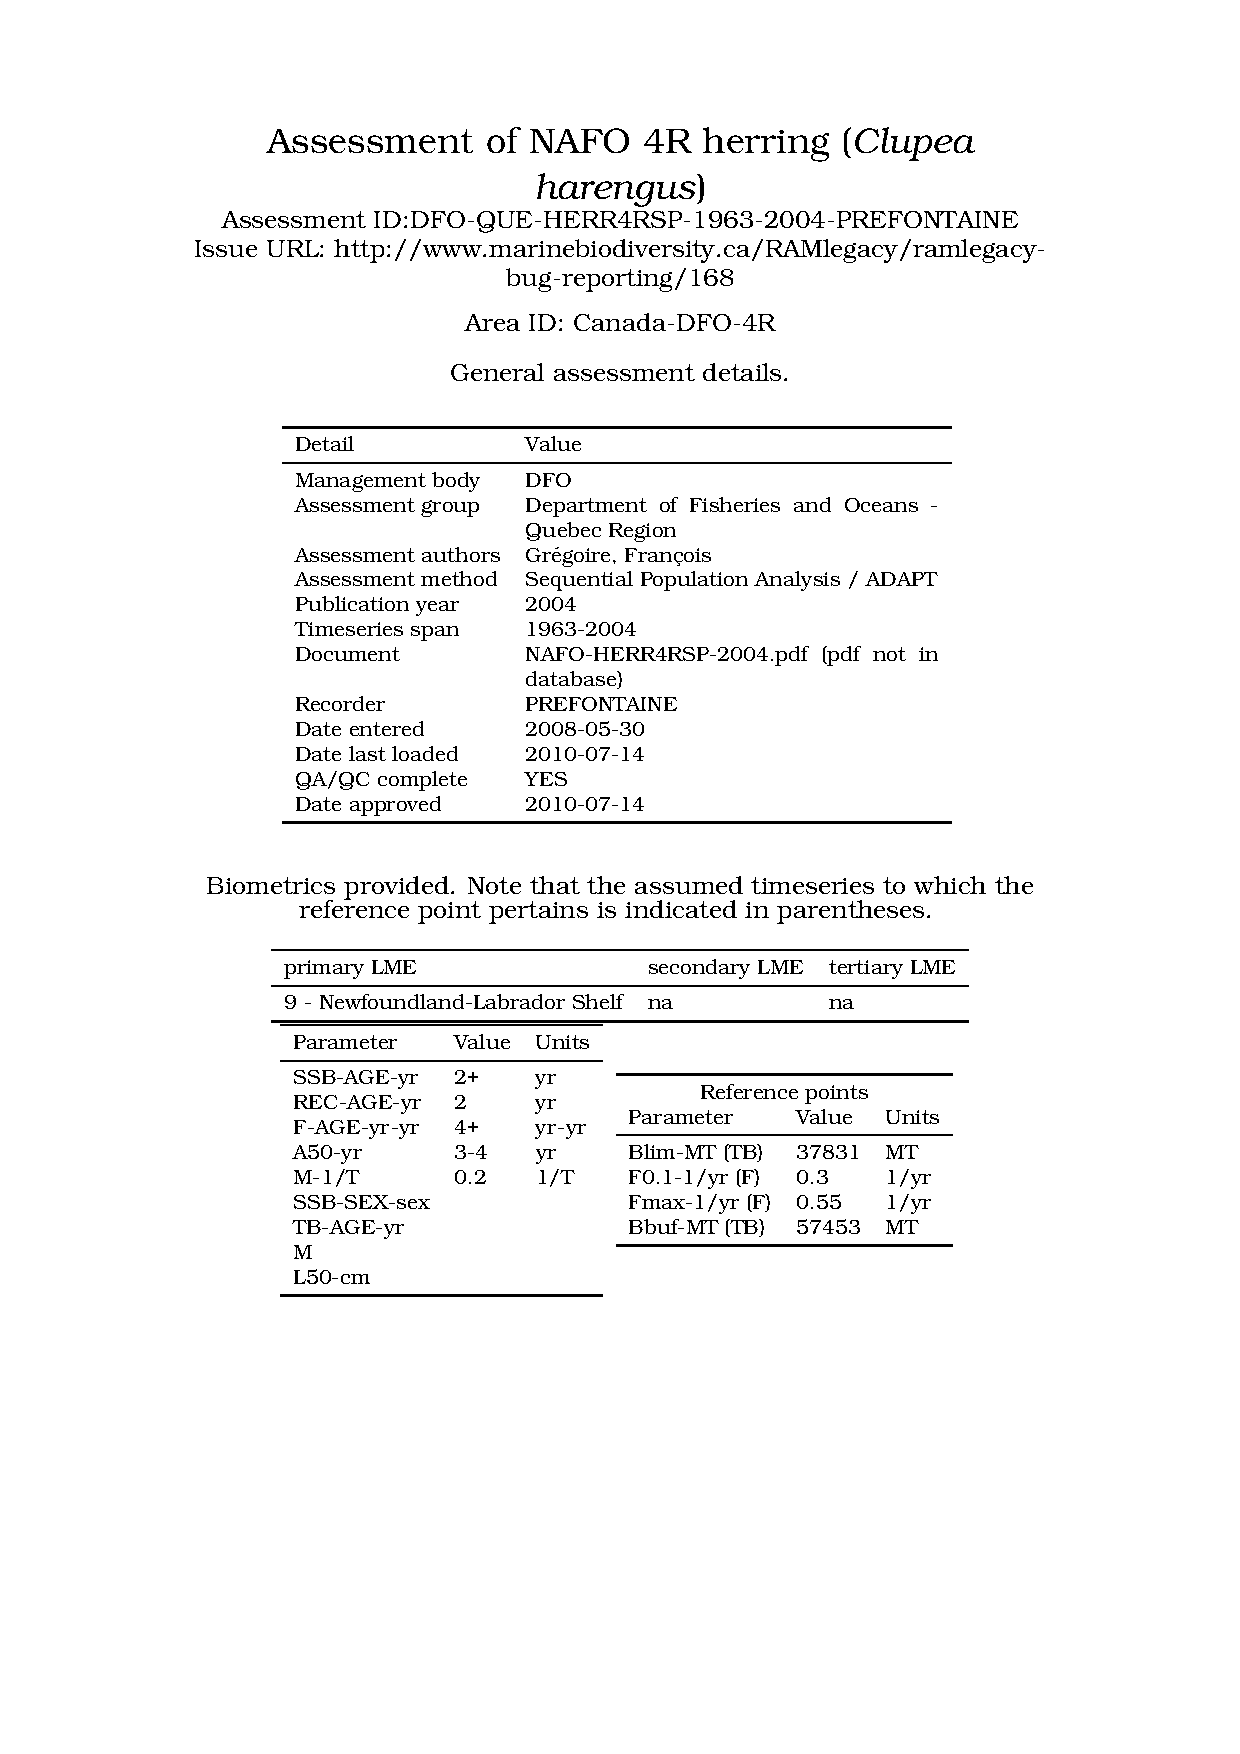
\includepdf[pagecommand={\thispagestyle{plain}}, pages={1,2}]{../../../tex/DFO-QUE-HERR4RSP-1963-2004-PREFONTAINE.pdf}
\index{Herring}\index{Clupea harengus}\index{Clupeidae!Clupea harengus}
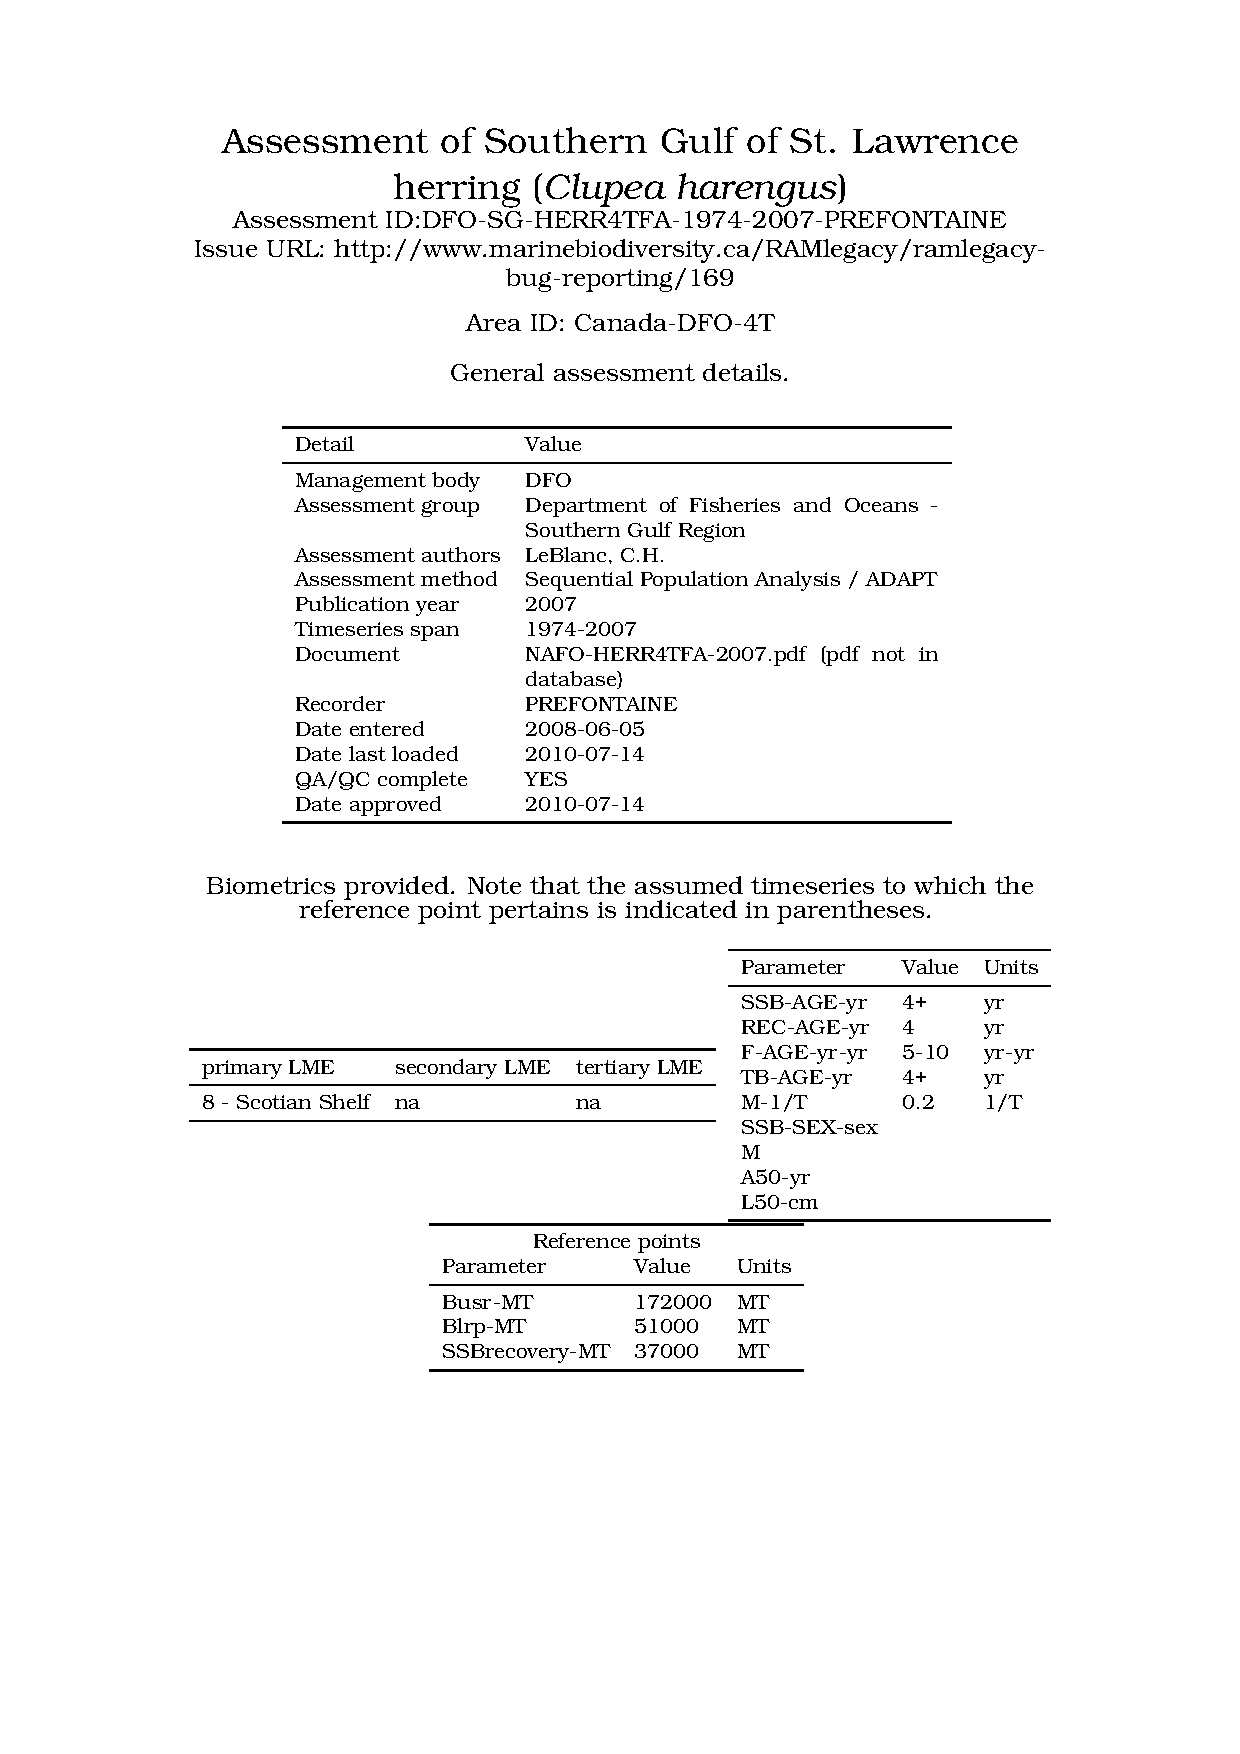
\includepdf[pagecommand={\thispagestyle{plain}}, pages={1,2}]{../../../tex/DFO-SG-HERR4TFA-1974-2007-PREFONTAINE.pdf}
\index{Herring}\index{Clupea harengus}\index{Clupeidae!Clupea harengus}
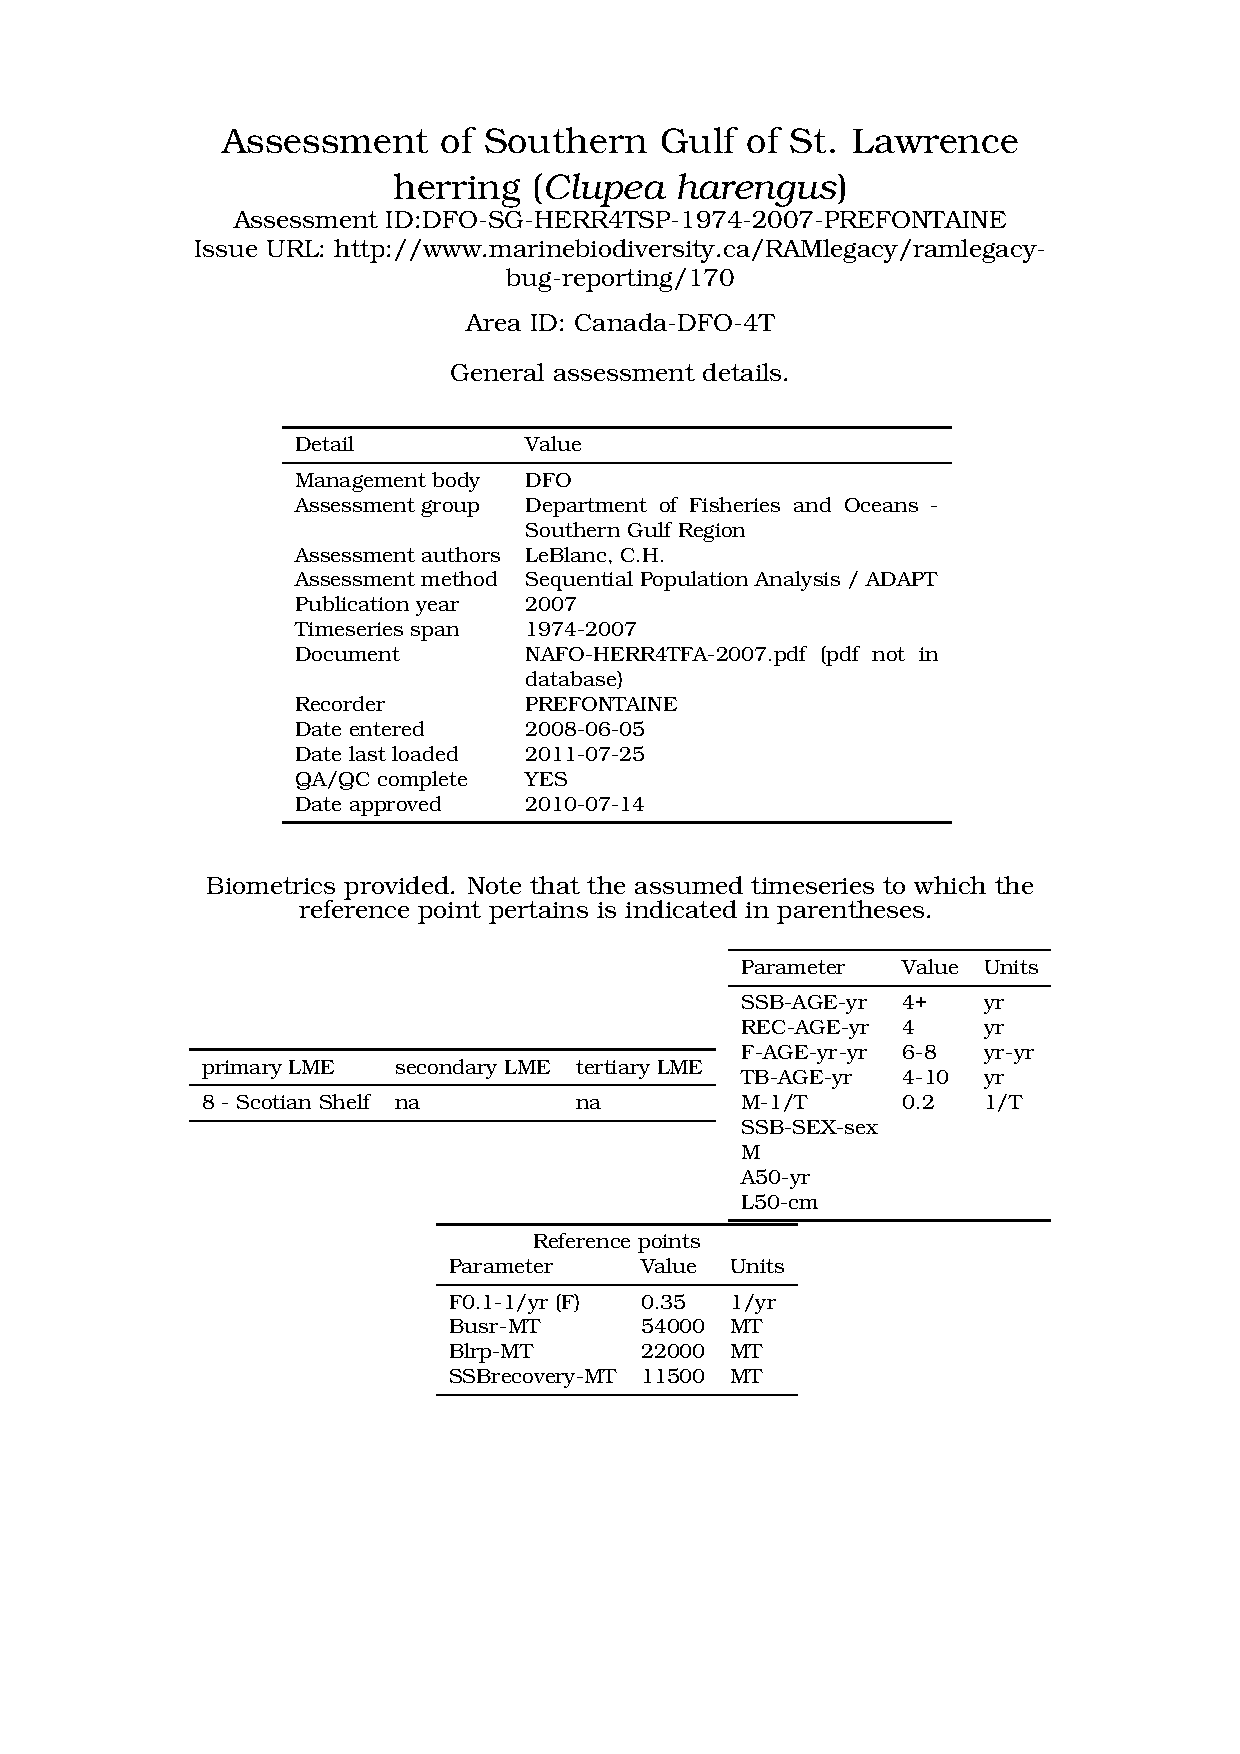
\includepdf[pagecommand={\thispagestyle{plain}}, pages={1,2}]{../../../tex/DFO-SG-HERR4TSP-1974-2007-PREFONTAINE.pdf}
\index{Herring}\index{Clupea harengus}\index{Clupeidae!Clupea harengus}
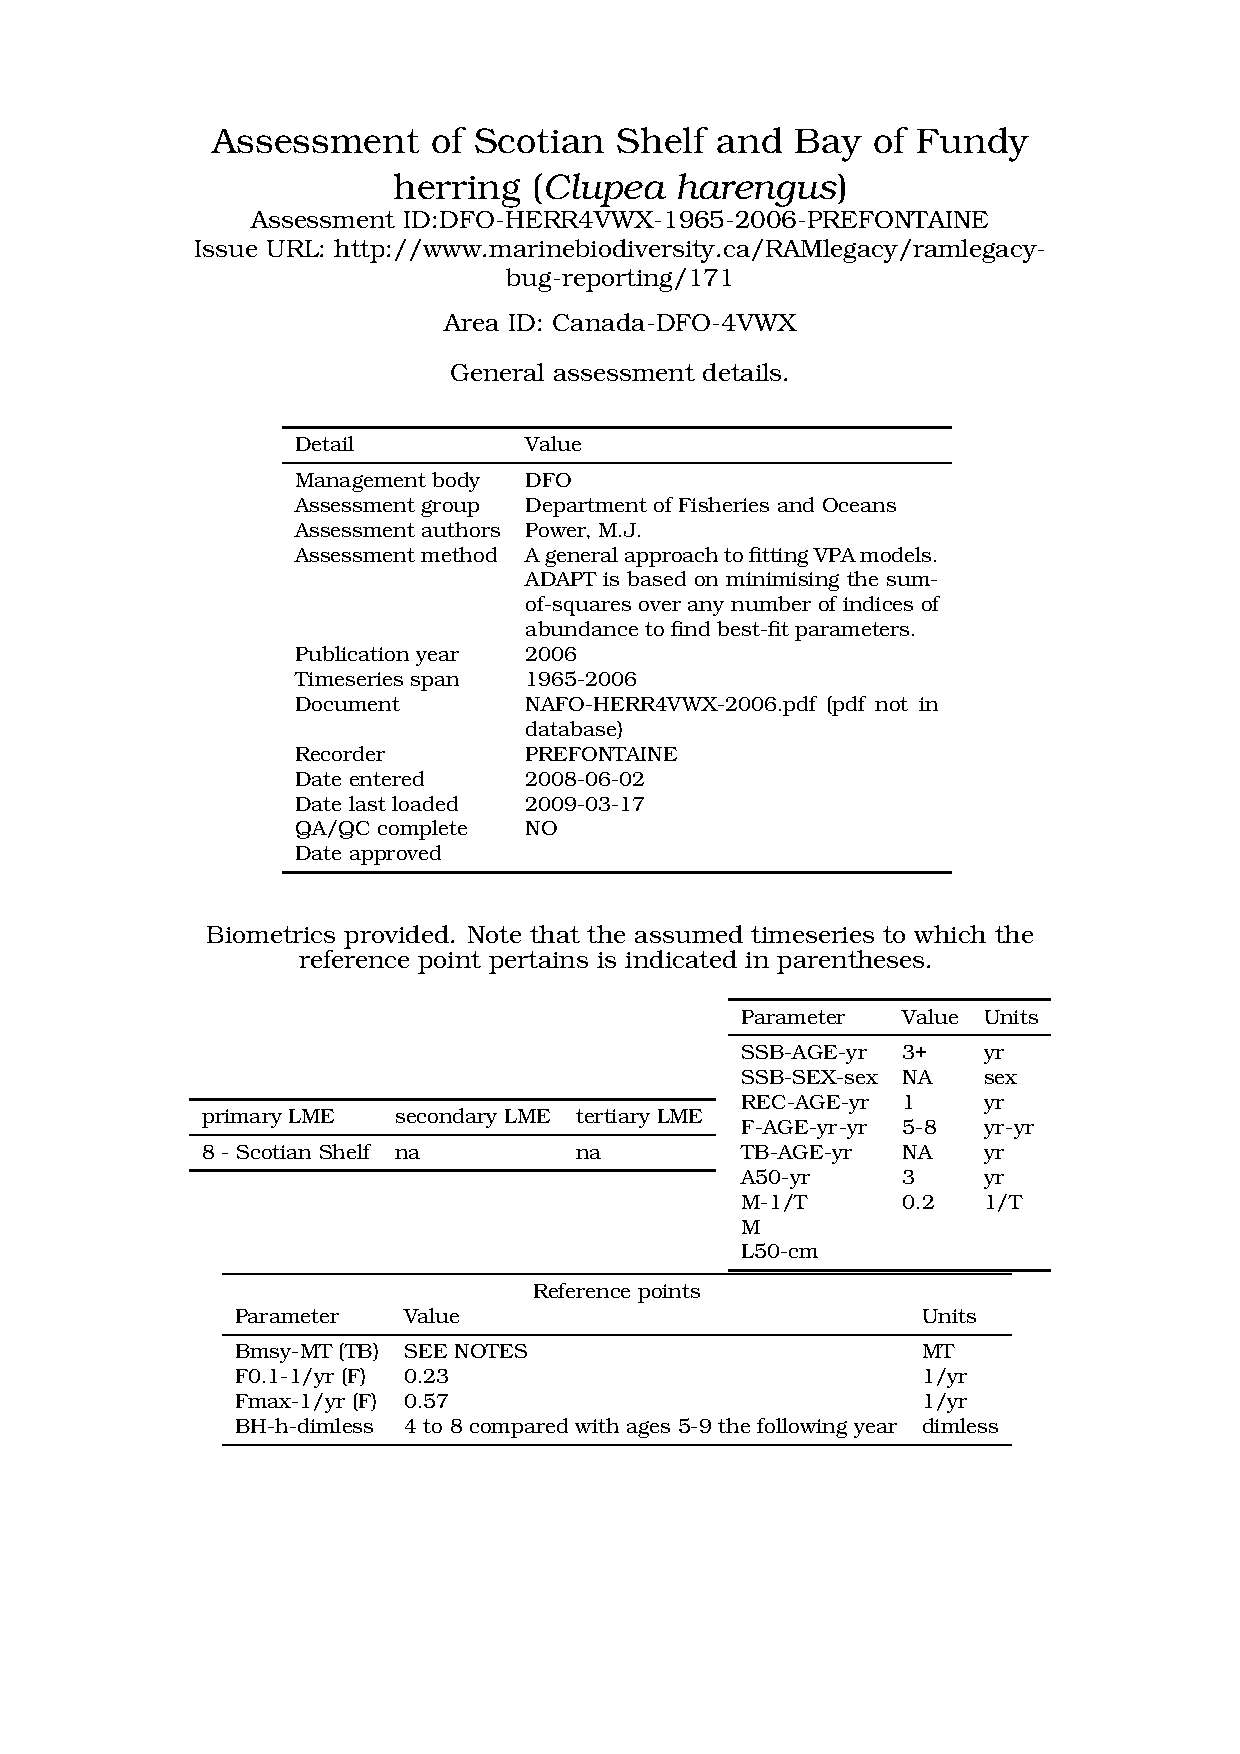
\includepdf[pagecommand={\thispagestyle{plain}}, pages={1,2}]{../../../tex/DFO-HERR4VWX-1965-2006-PREFONTAINE.pdf}
\index{Pacific herring}\index{Clupea pallasii}\index{Clupeidae!Clupea pallasii}
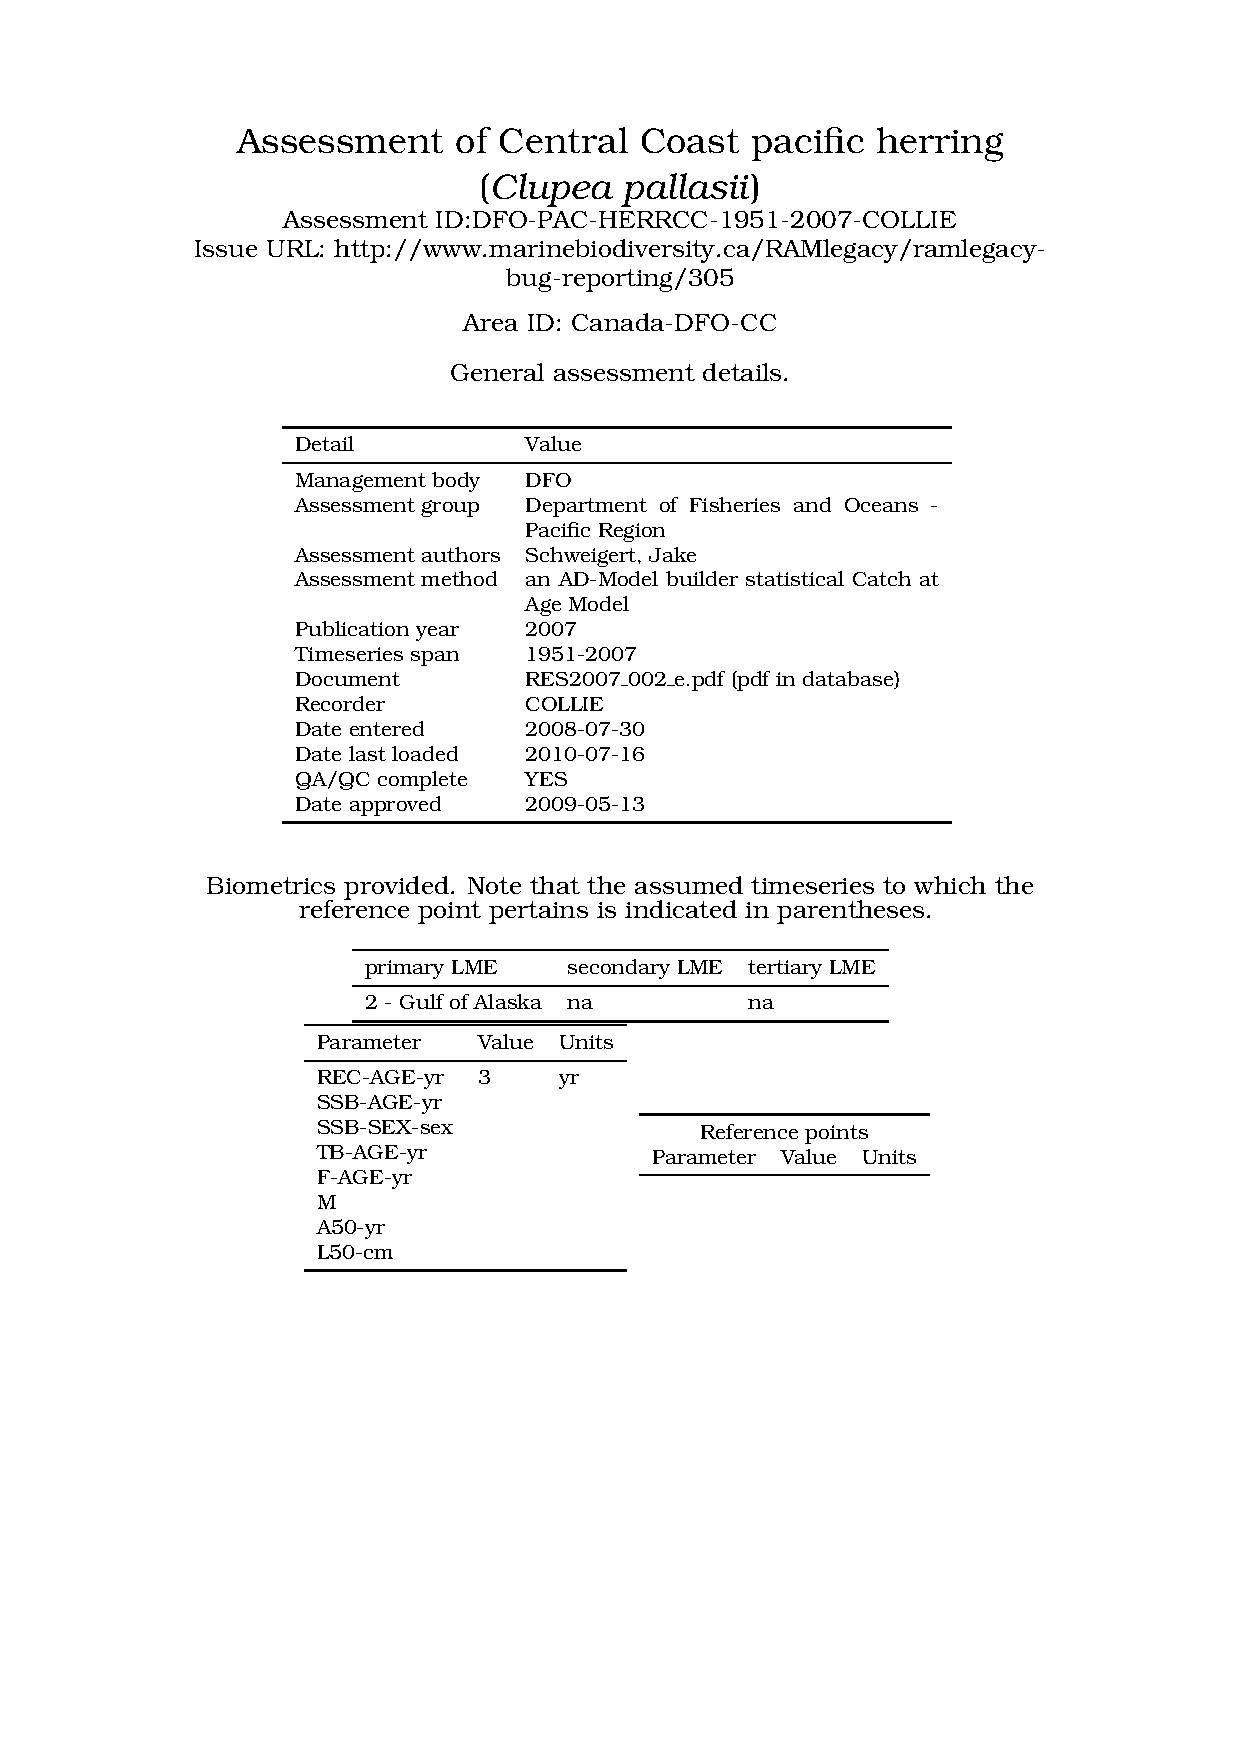
\includepdf[pagecommand={\thispagestyle{plain}}, pages={1,2}]{../../../tex/DFO-PAC-HERRCC-1951-2007-COLLIE.pdf}
\index{Pacific herring}\index{Clupea pallasii}\index{Clupeidae!Clupea pallasii}
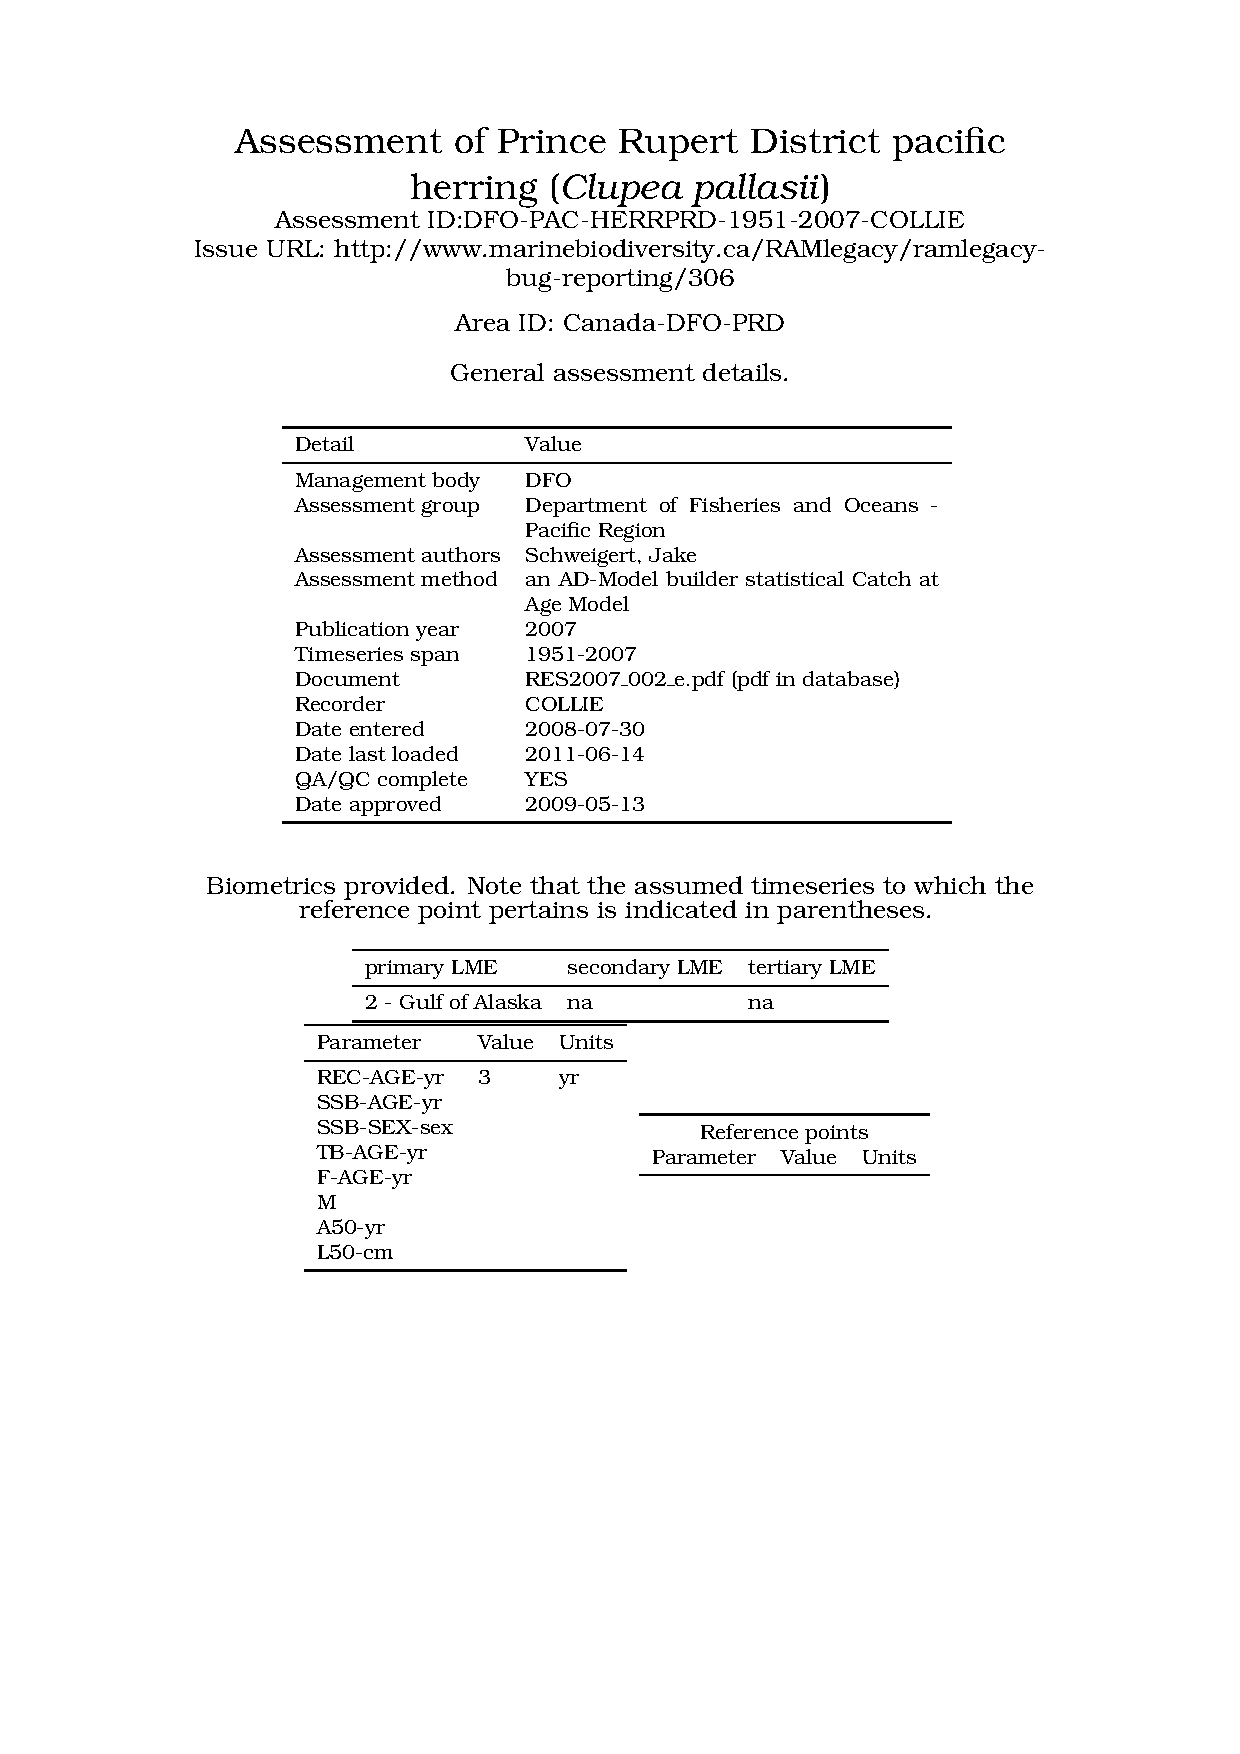
\includepdf[pagecommand={\thispagestyle{plain}}, pages={1,2}]{../../../tex/DFO-PAC-HERRPRD-1951-2007-COLLIE.pdf}
\index{Pacific herring}\index{Clupea pallasii}\index{Clupeidae!Clupea pallasii}
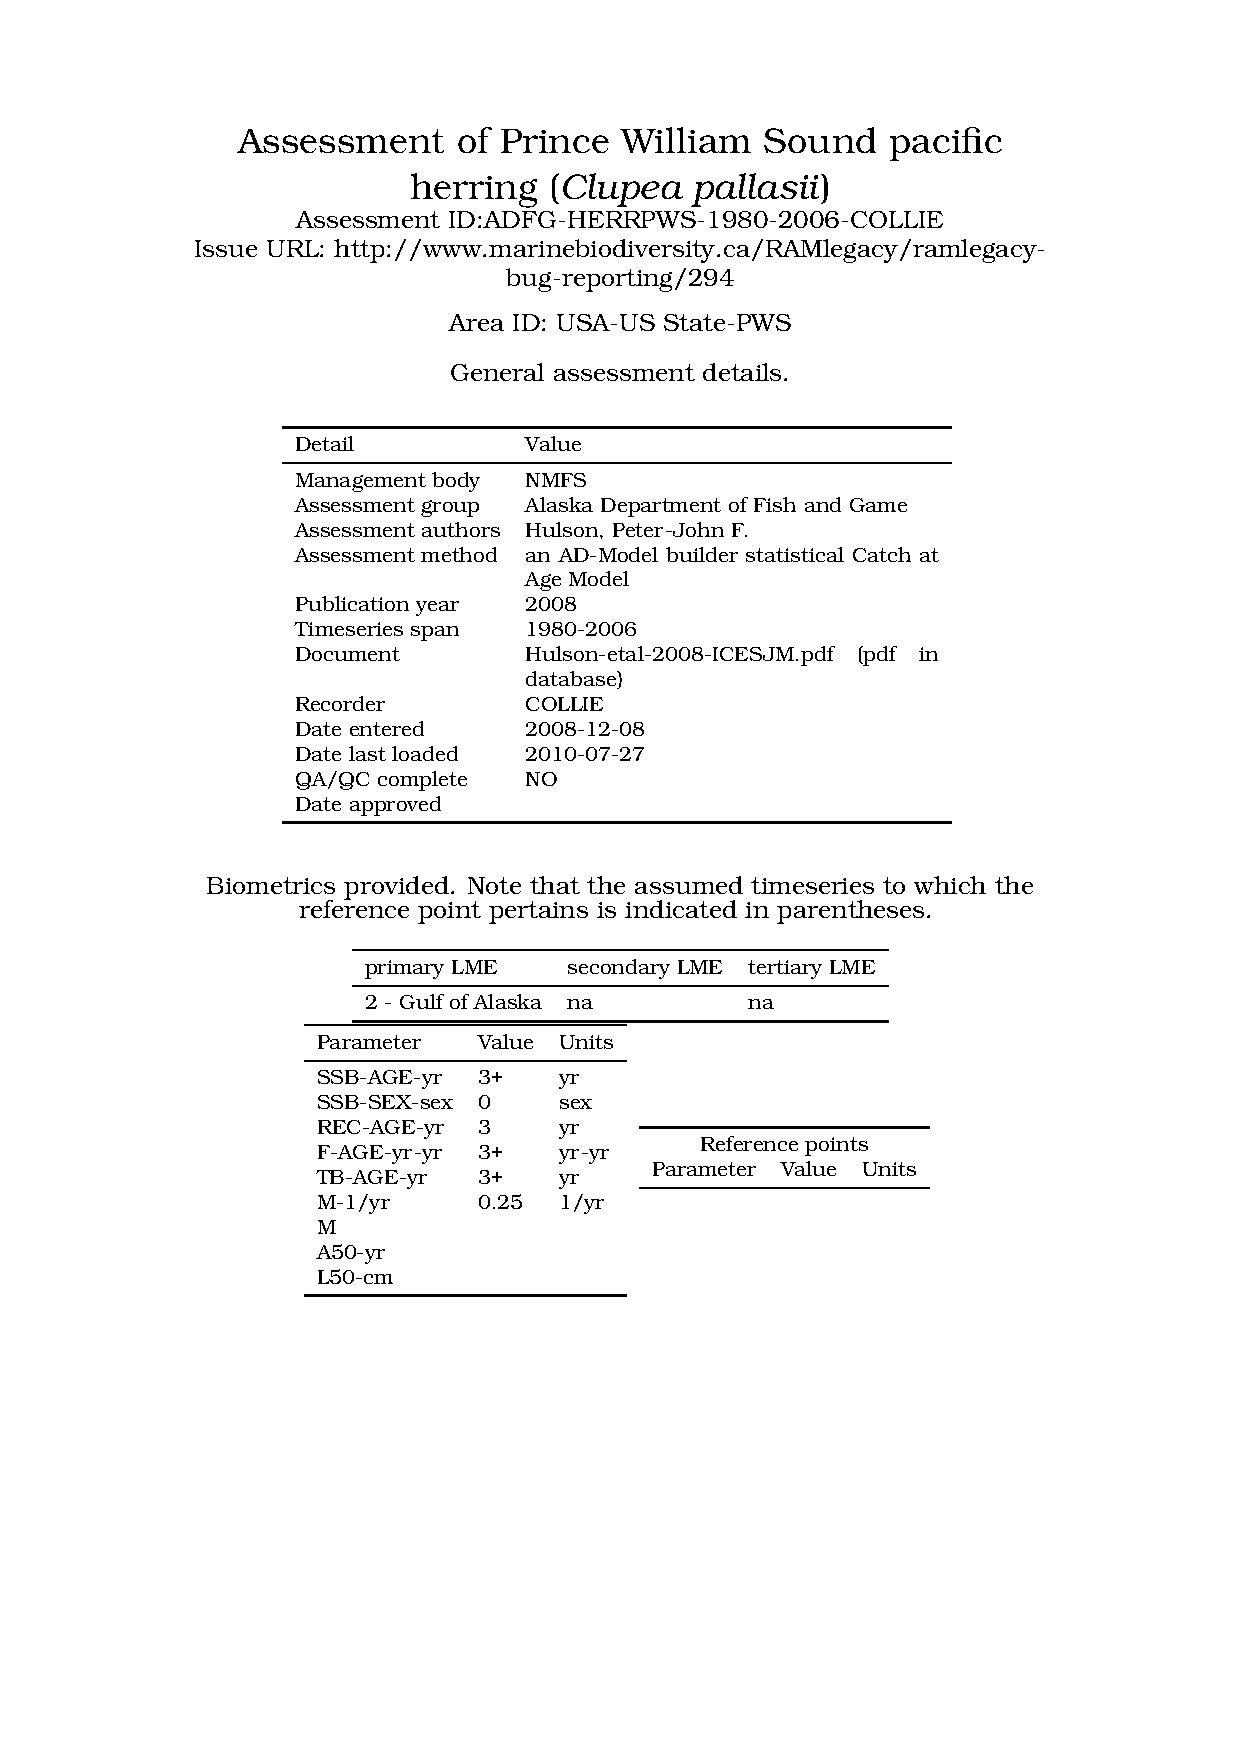
\includepdf[pagecommand={\thispagestyle{plain}}, pages={1,2}]{../../../tex/ADFG-HERRPWS-1980-2006-COLLIE.pdf}
\index{Pacific herring}\index{Clupea pallasii}\index{Clupeidae!Clupea pallasii}
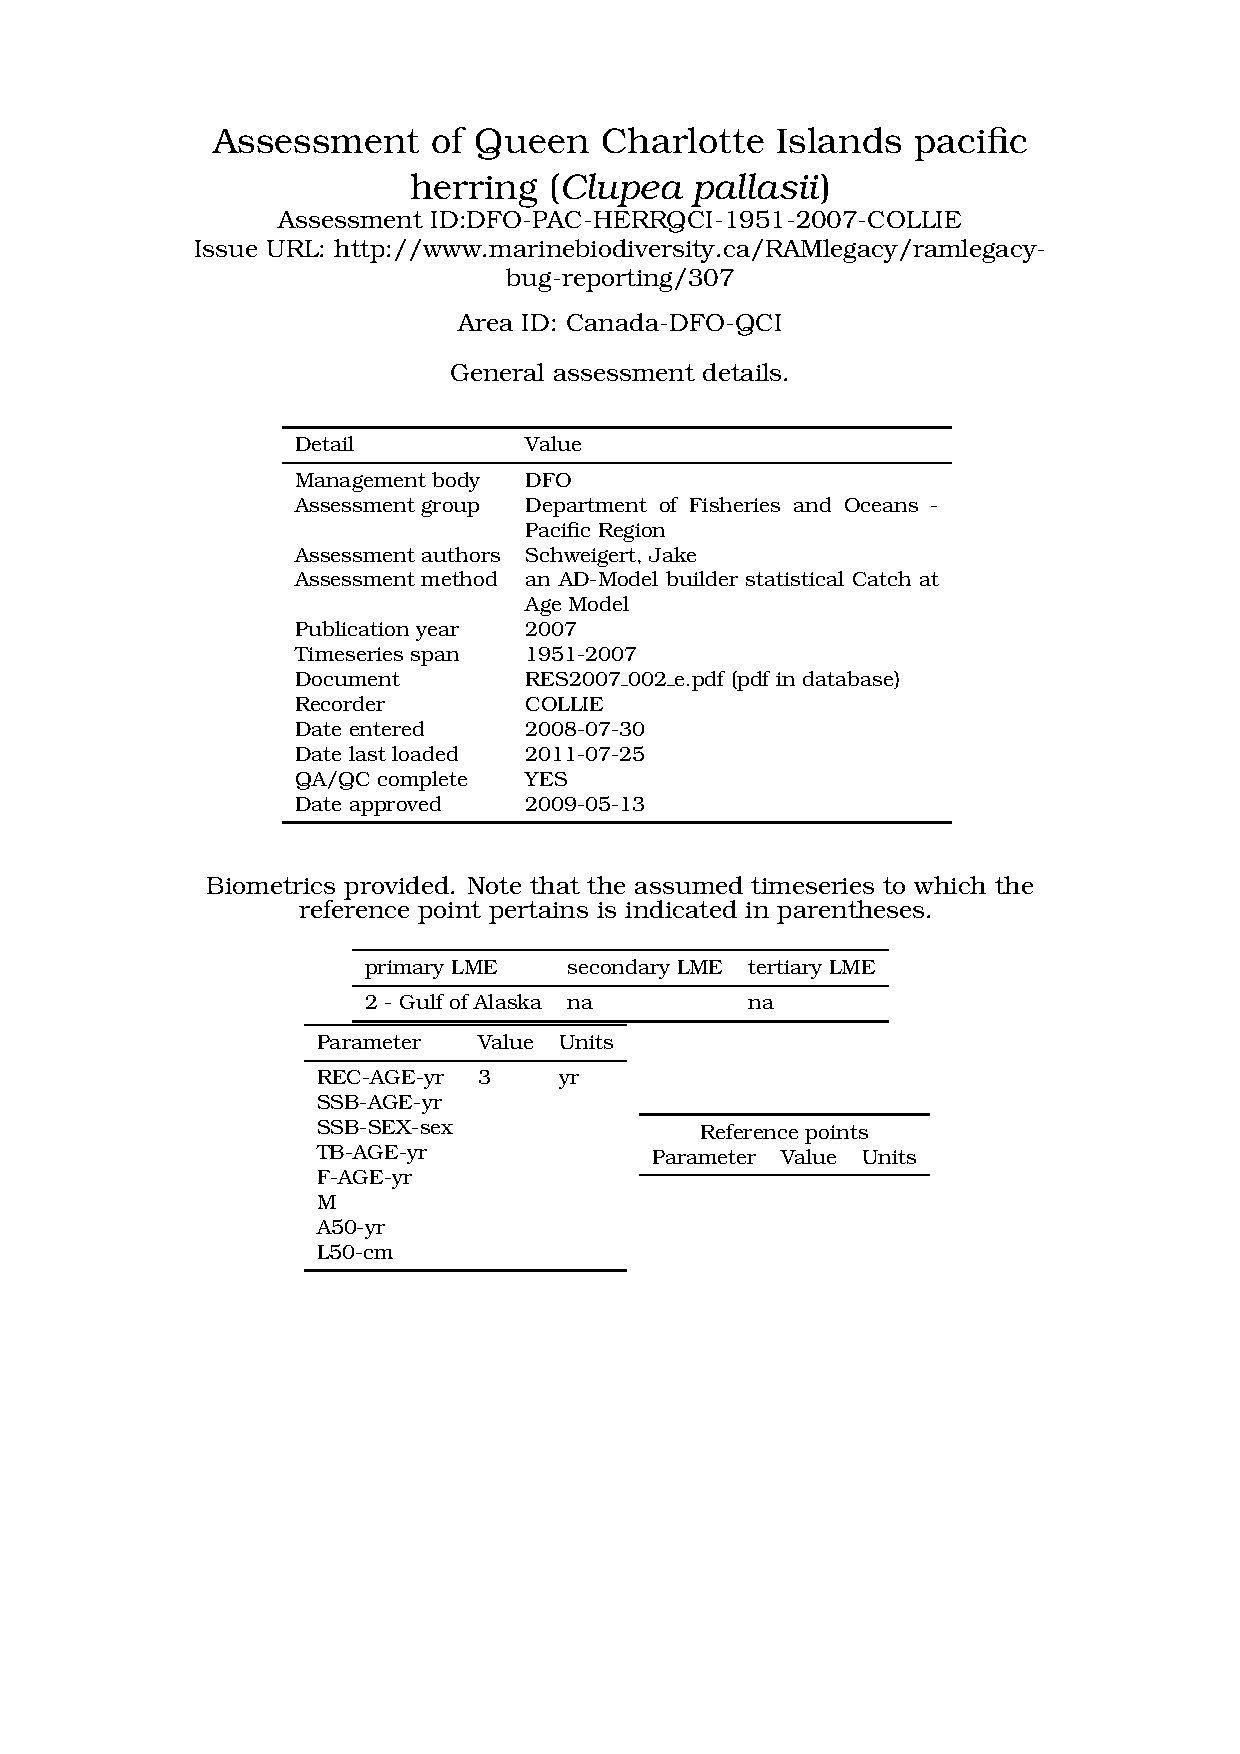
\includepdf[pagecommand={\thispagestyle{plain}}, pages={1,2}]{../../../tex/DFO-PAC-HERRQCI-1951-2007-COLLIE.pdf}
\index{Pacific herring}\index{Clupea pallasii}\index{Clupeidae!Clupea pallasii}
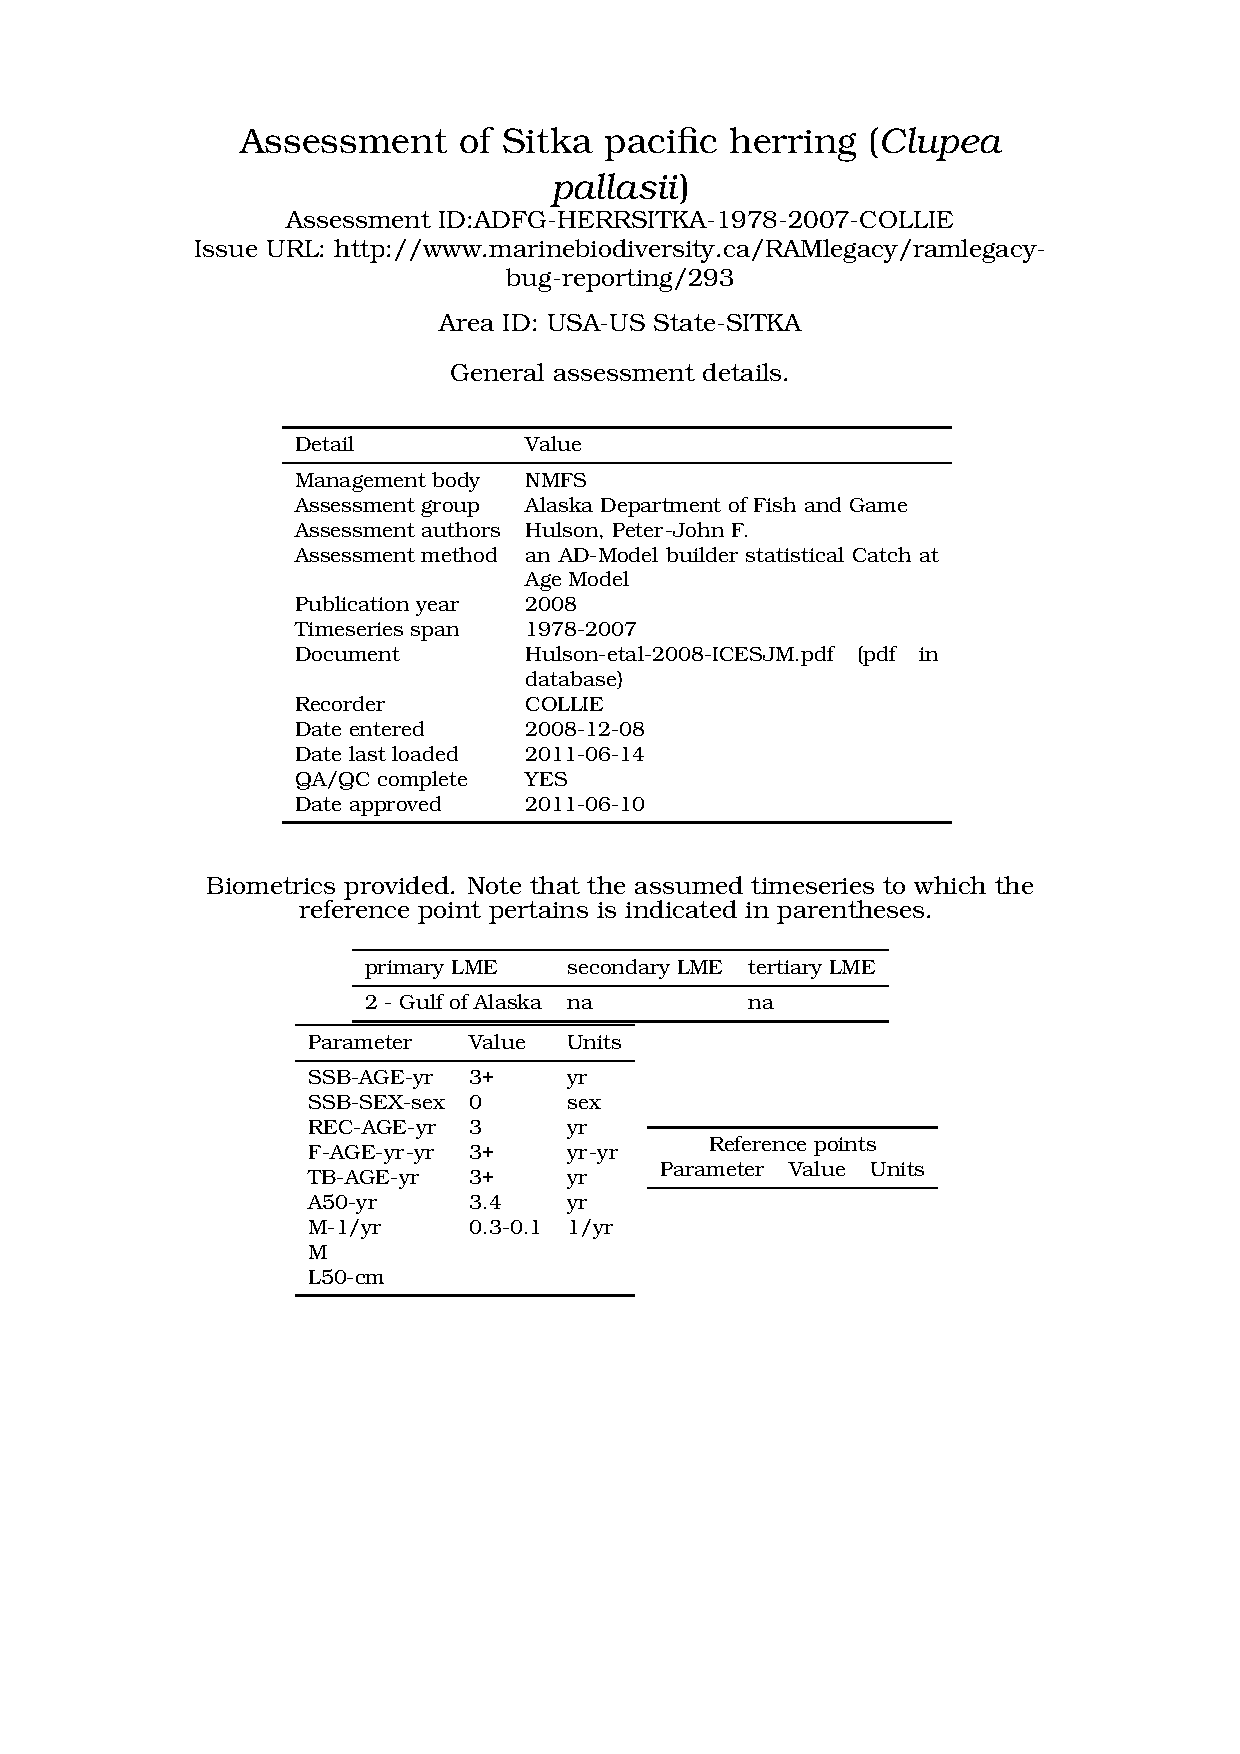
\includepdf[pagecommand={\thispagestyle{plain}}, pages={1,2}]{../../../tex/ADFG-HERRSITKA-1978-2007-COLLIE.pdf}
\index{Pacific herring}\index{Clupea pallasii}\index{Clupeidae!Clupea pallasii}
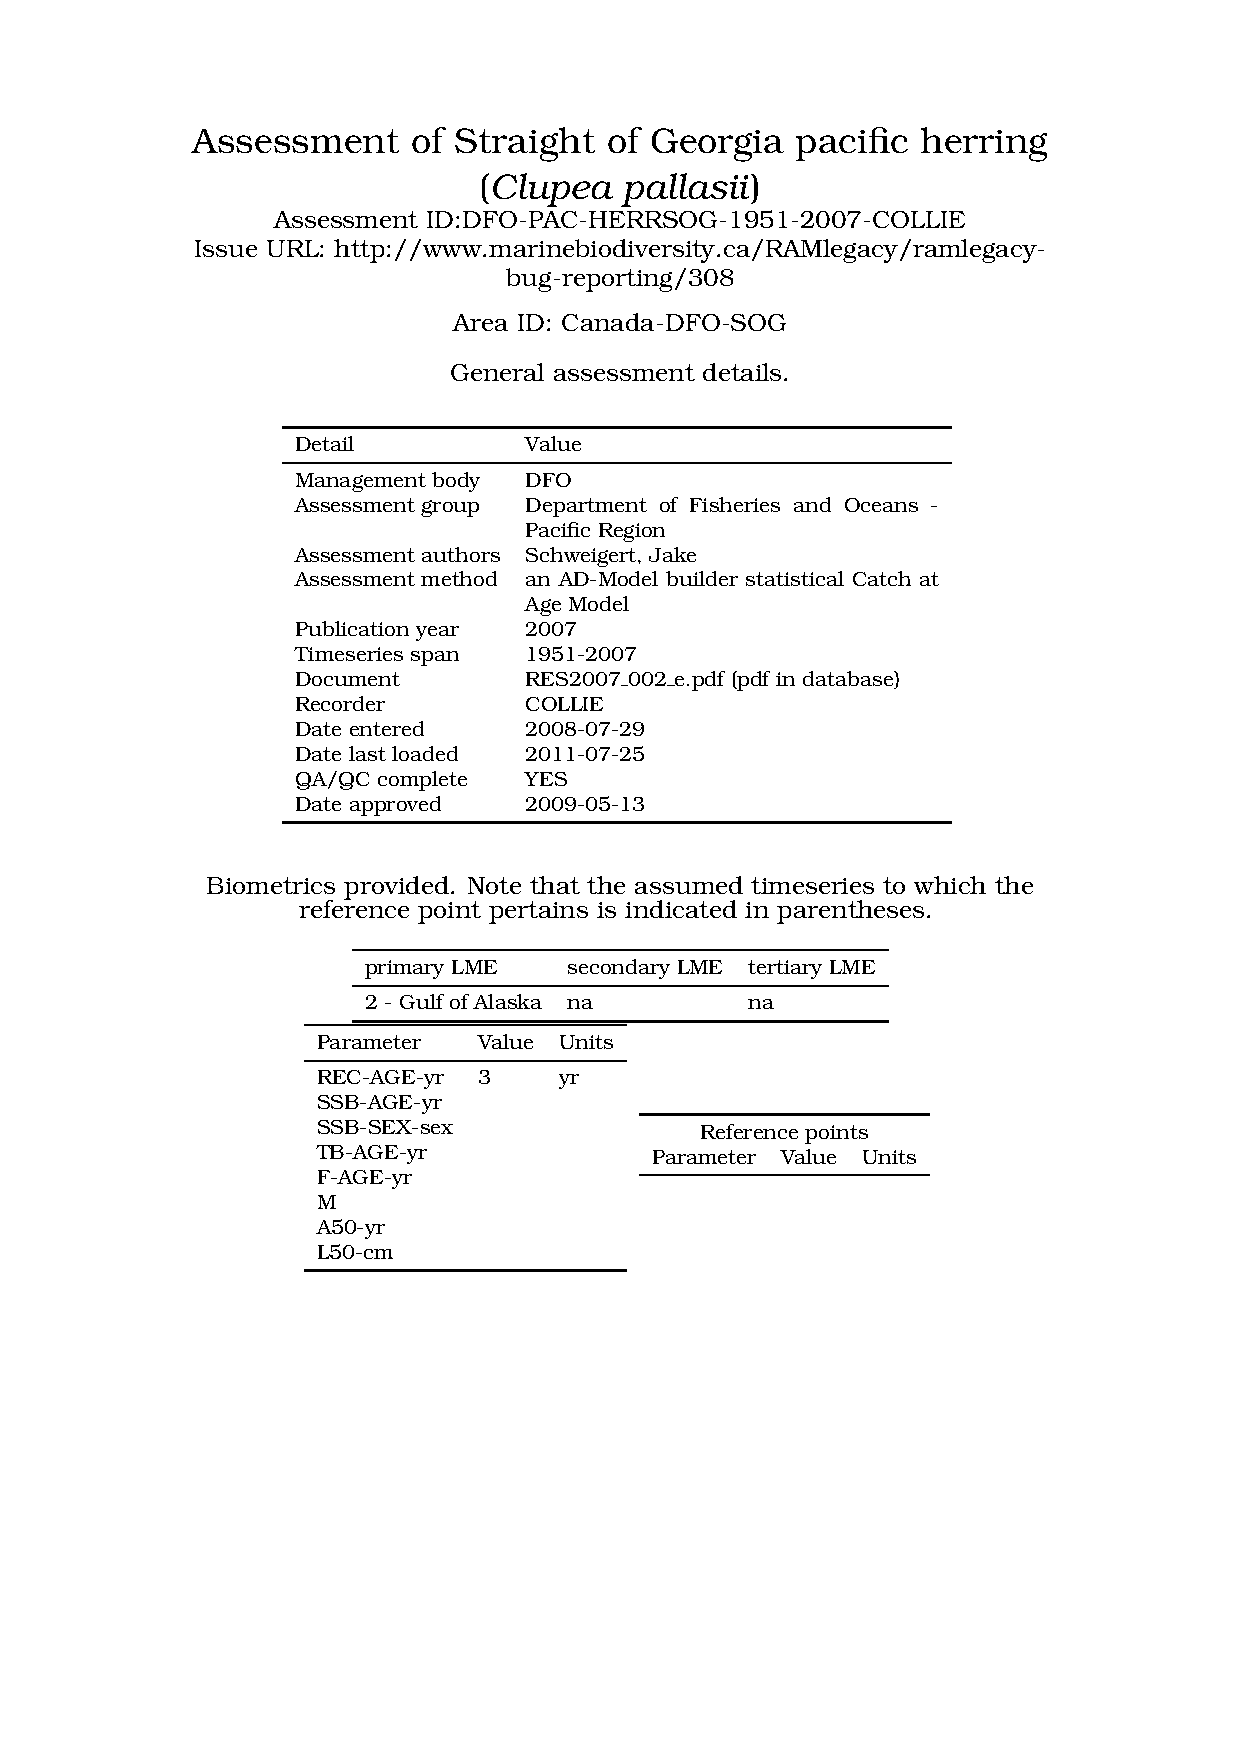
\includepdf[pagecommand={\thispagestyle{plain}}, pages={1,2}]{../../../tex/DFO-PAC-HERRSOG-1951-2007-COLLIE.pdf}
\index{Pacific herring}\index{Clupea pallasii}\index{Clupeidae!Clupea pallasii}
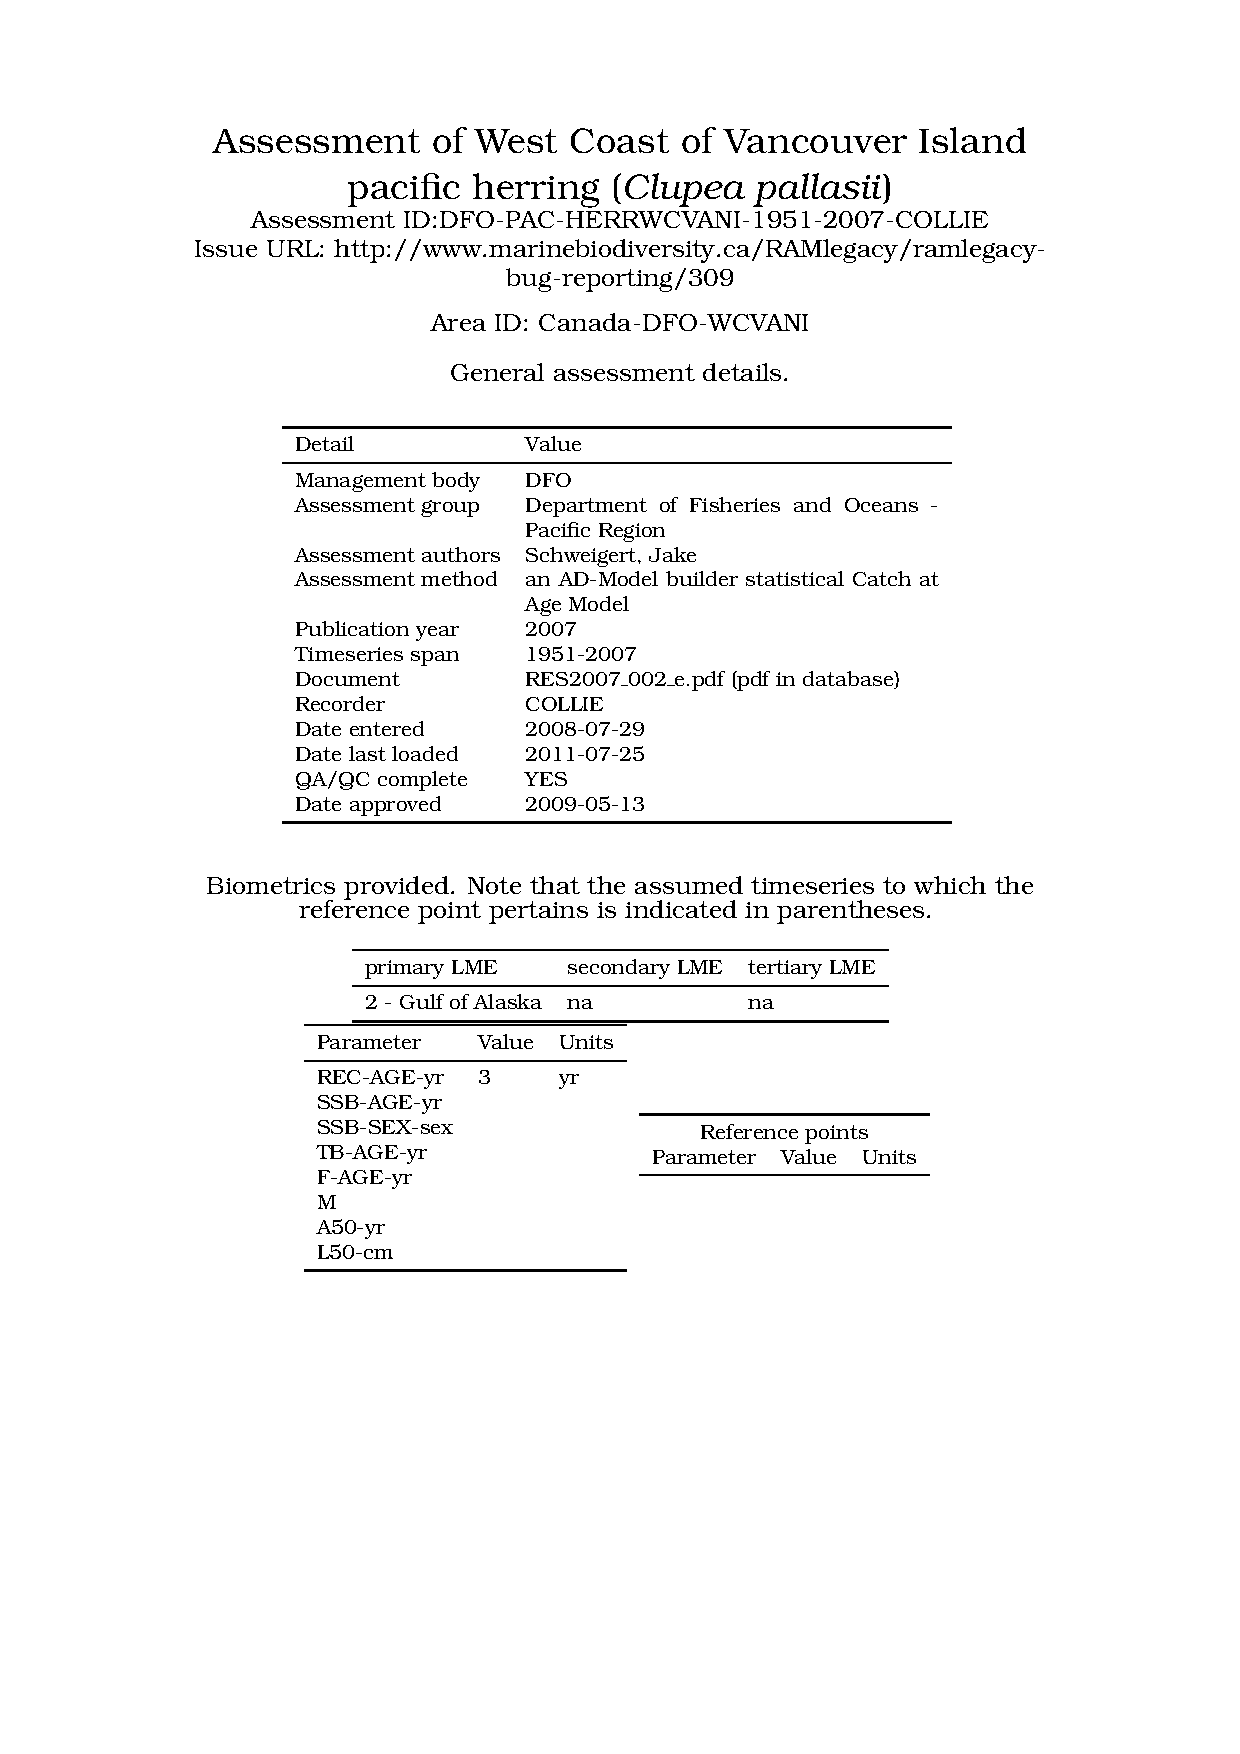
\includepdf[pagecommand={\thispagestyle{plain}}, pages={1,2}]{../../../tex/DFO-PAC-HERRWCVANI-1951-2007-COLLIE.pdf}
\index{European pilchard}\index{Sardina pilchardus}\index{Clupeidae!Sardina pilchardus}
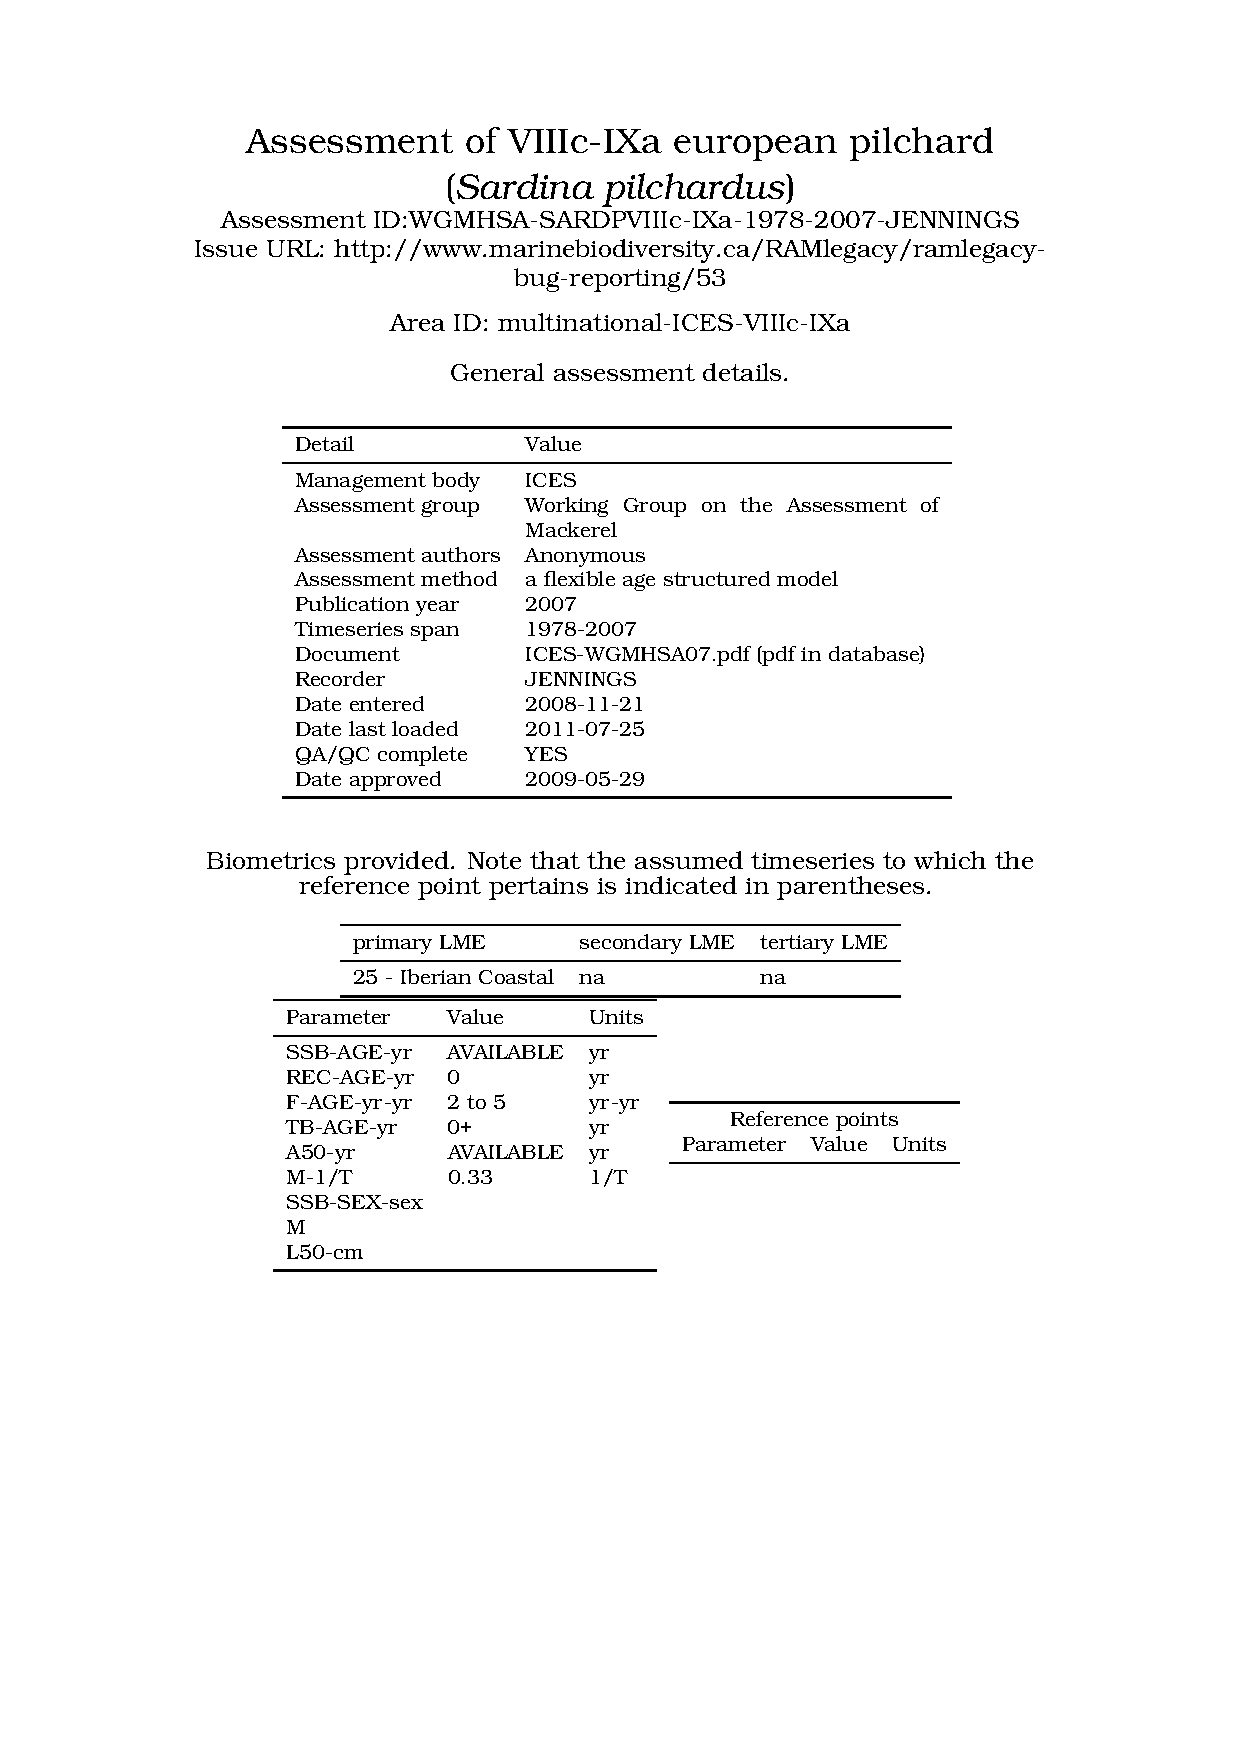
\includepdf[pagecommand={\thispagestyle{plain}}, pages={1,2}]{../../../tex/WGMHSA-SARDPVIIIc-IXa-1978-2007-JENNINGS.pdf}
\index{Sardine}\index{Sardinops sagax}\index{Clupeidae!Sardinops sagax}
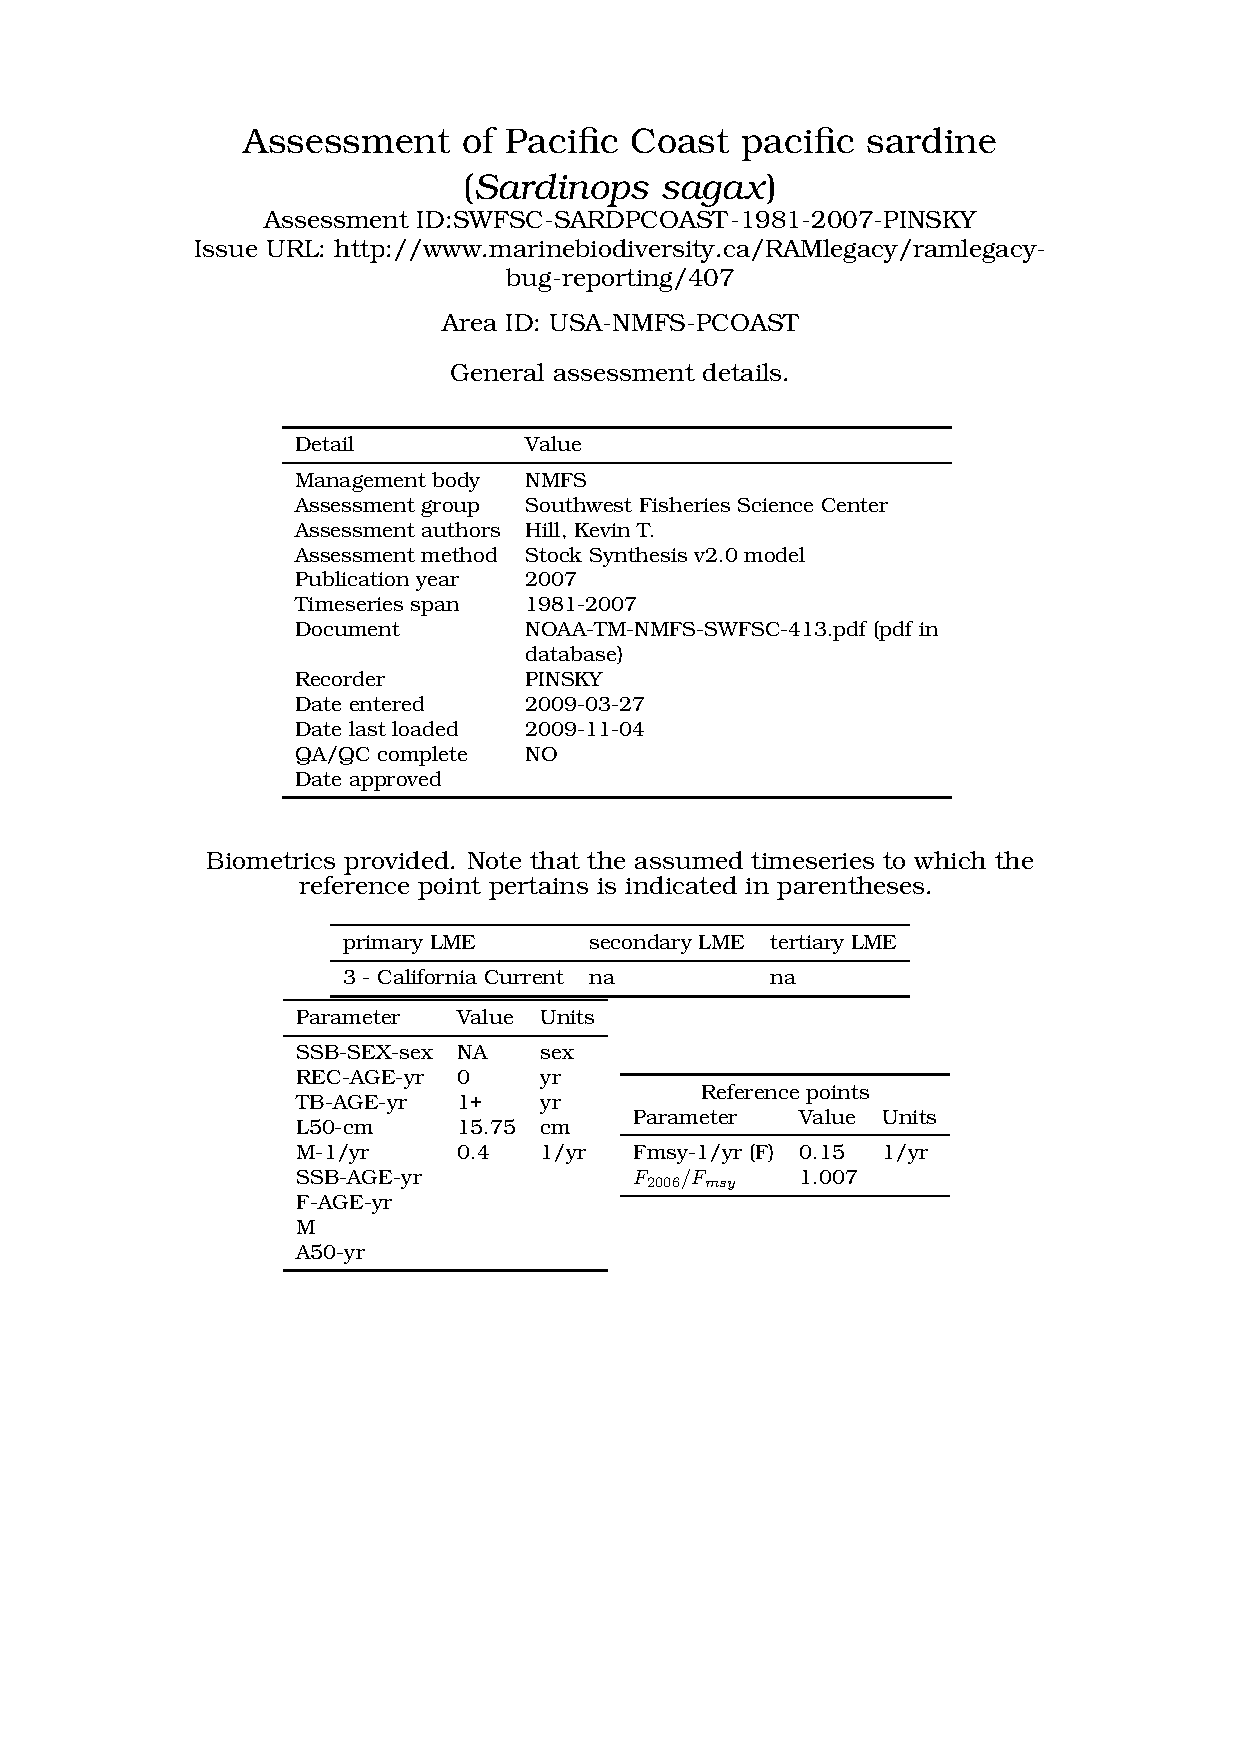
\includepdf[pagecommand={\thispagestyle{plain}}, pages={1,2}]{../../../tex/SWFSC-SARDPCOAST-1981-2007-PINSKY.pdf}
\index{Sardine}\index{Sardinops sagax}\index{Clupeidae!Sardinops sagax}
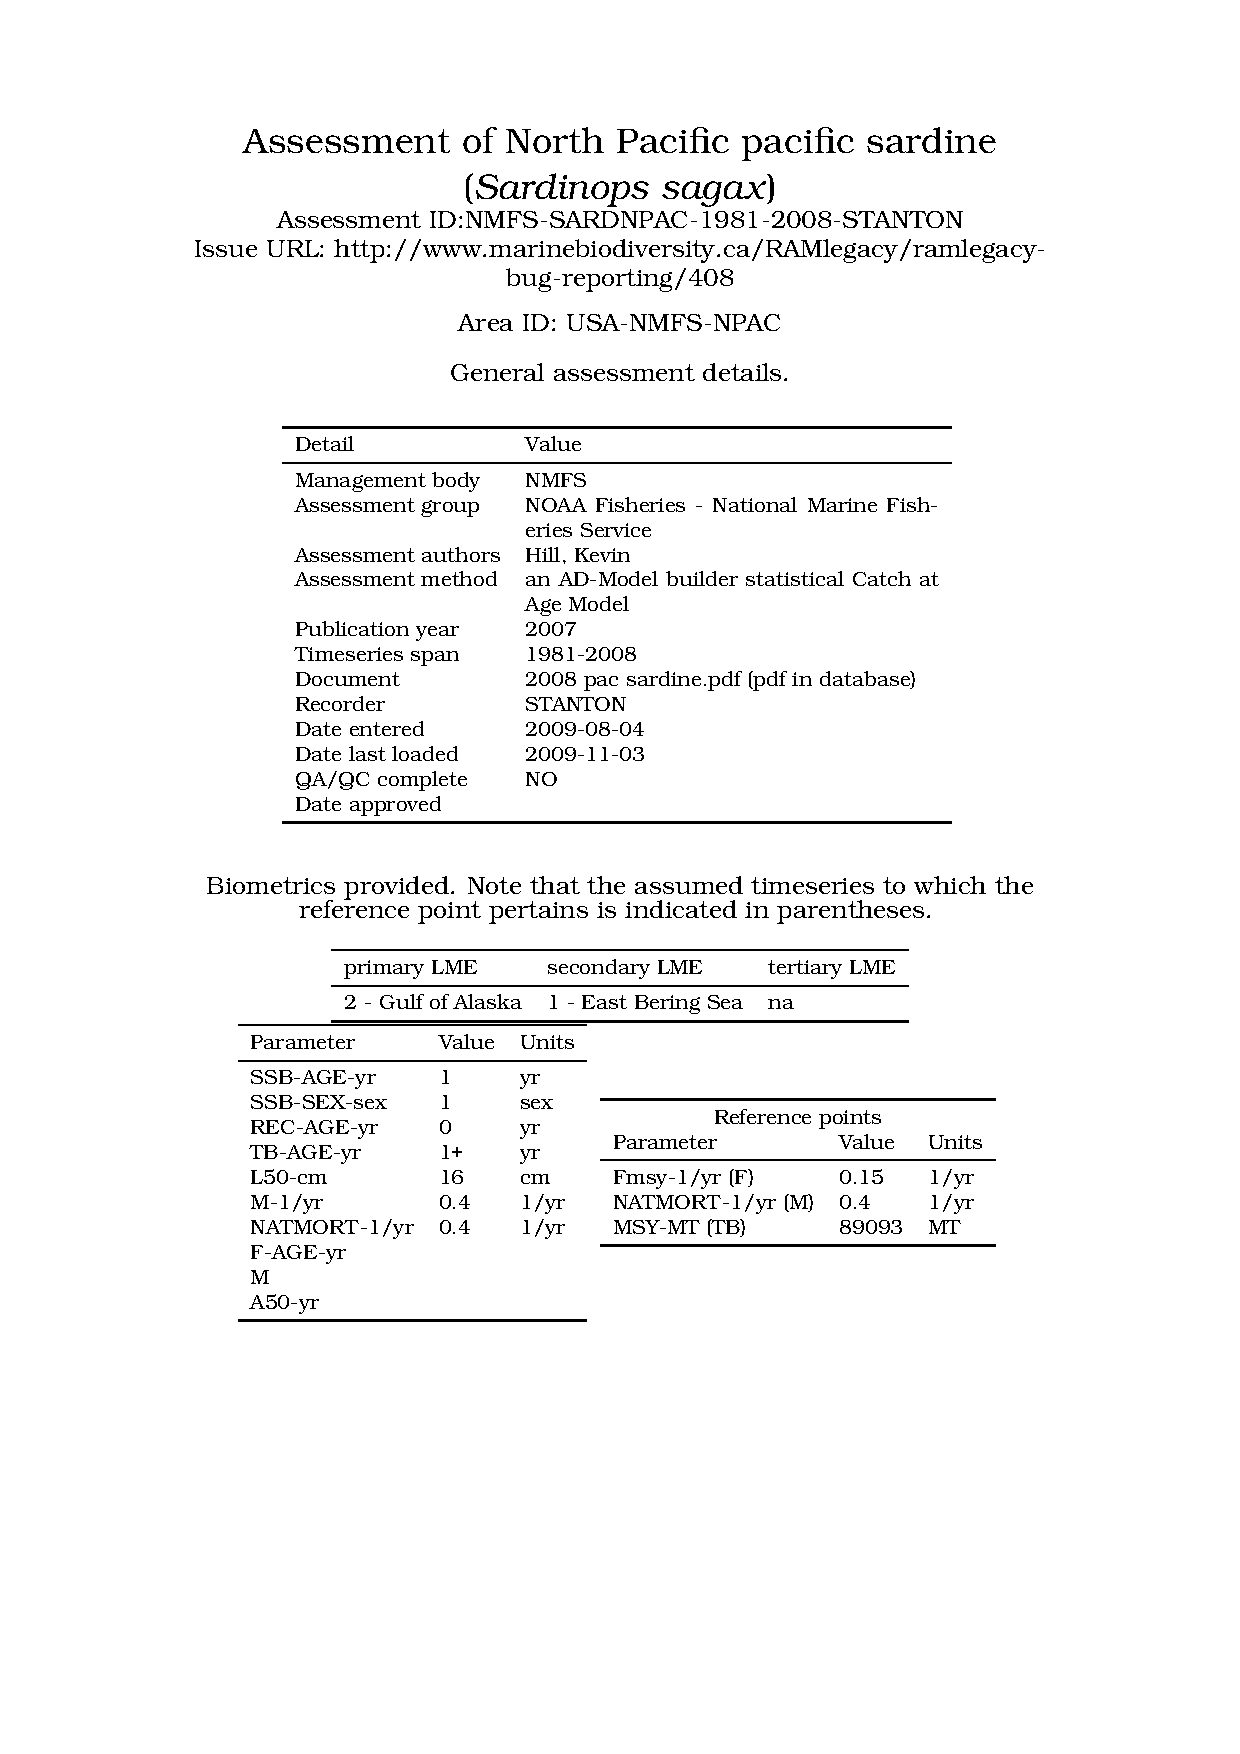
\includepdf[pagecommand={\thispagestyle{plain}}, pages={1,2}]{../../../tex/NMFS-SARDNPAC-1981-2008-STANTON.pdf}
\index{Sardine}\index{Sardinops sagax}\index{Clupeidae!Sardinops sagax}
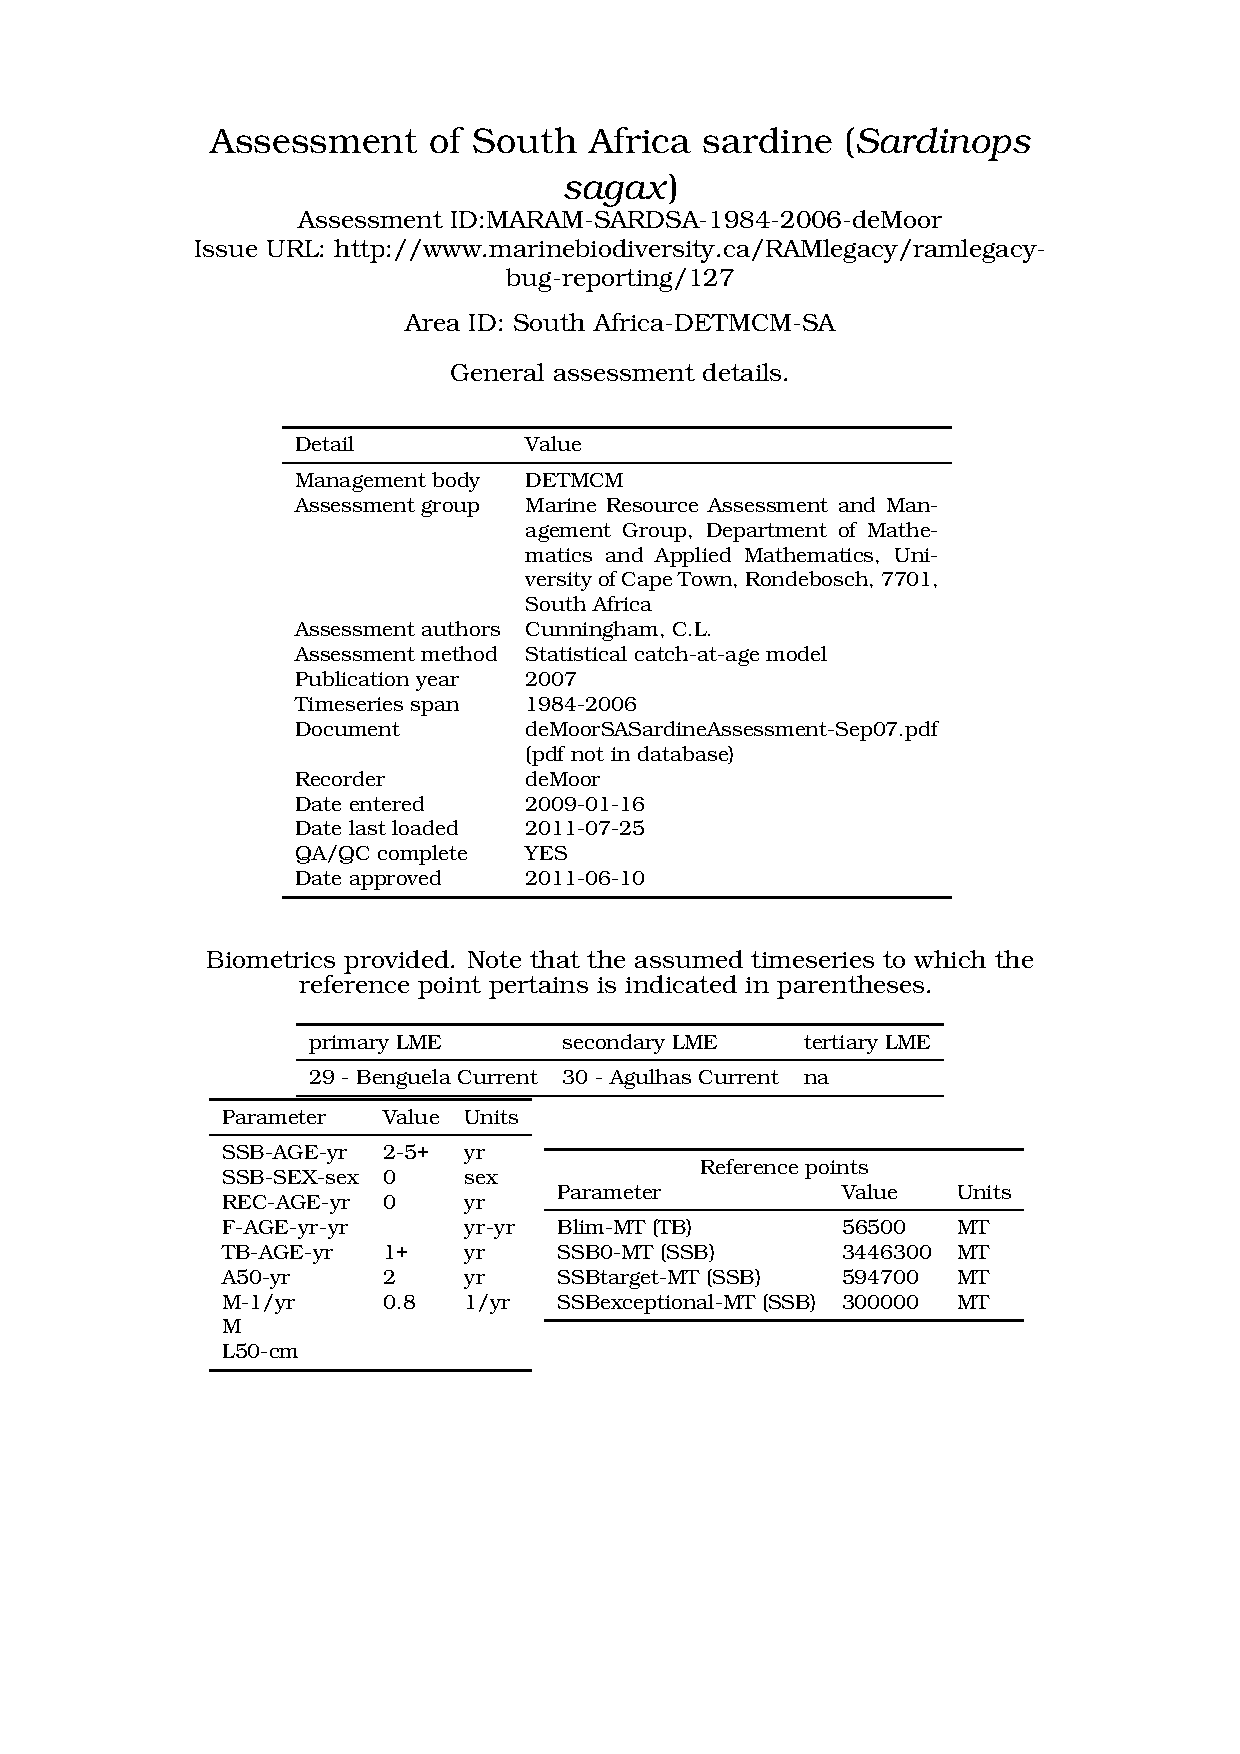
\includepdf[pagecommand={\thispagestyle{plain}}, pages={1,2}]{../../../tex/MARAM-SARDSA-1984-2006-deMoor.pdf}
\index{Sprat}\index{Sprattus sprattus}\index{Clupeidae!Sprattus sprattus}
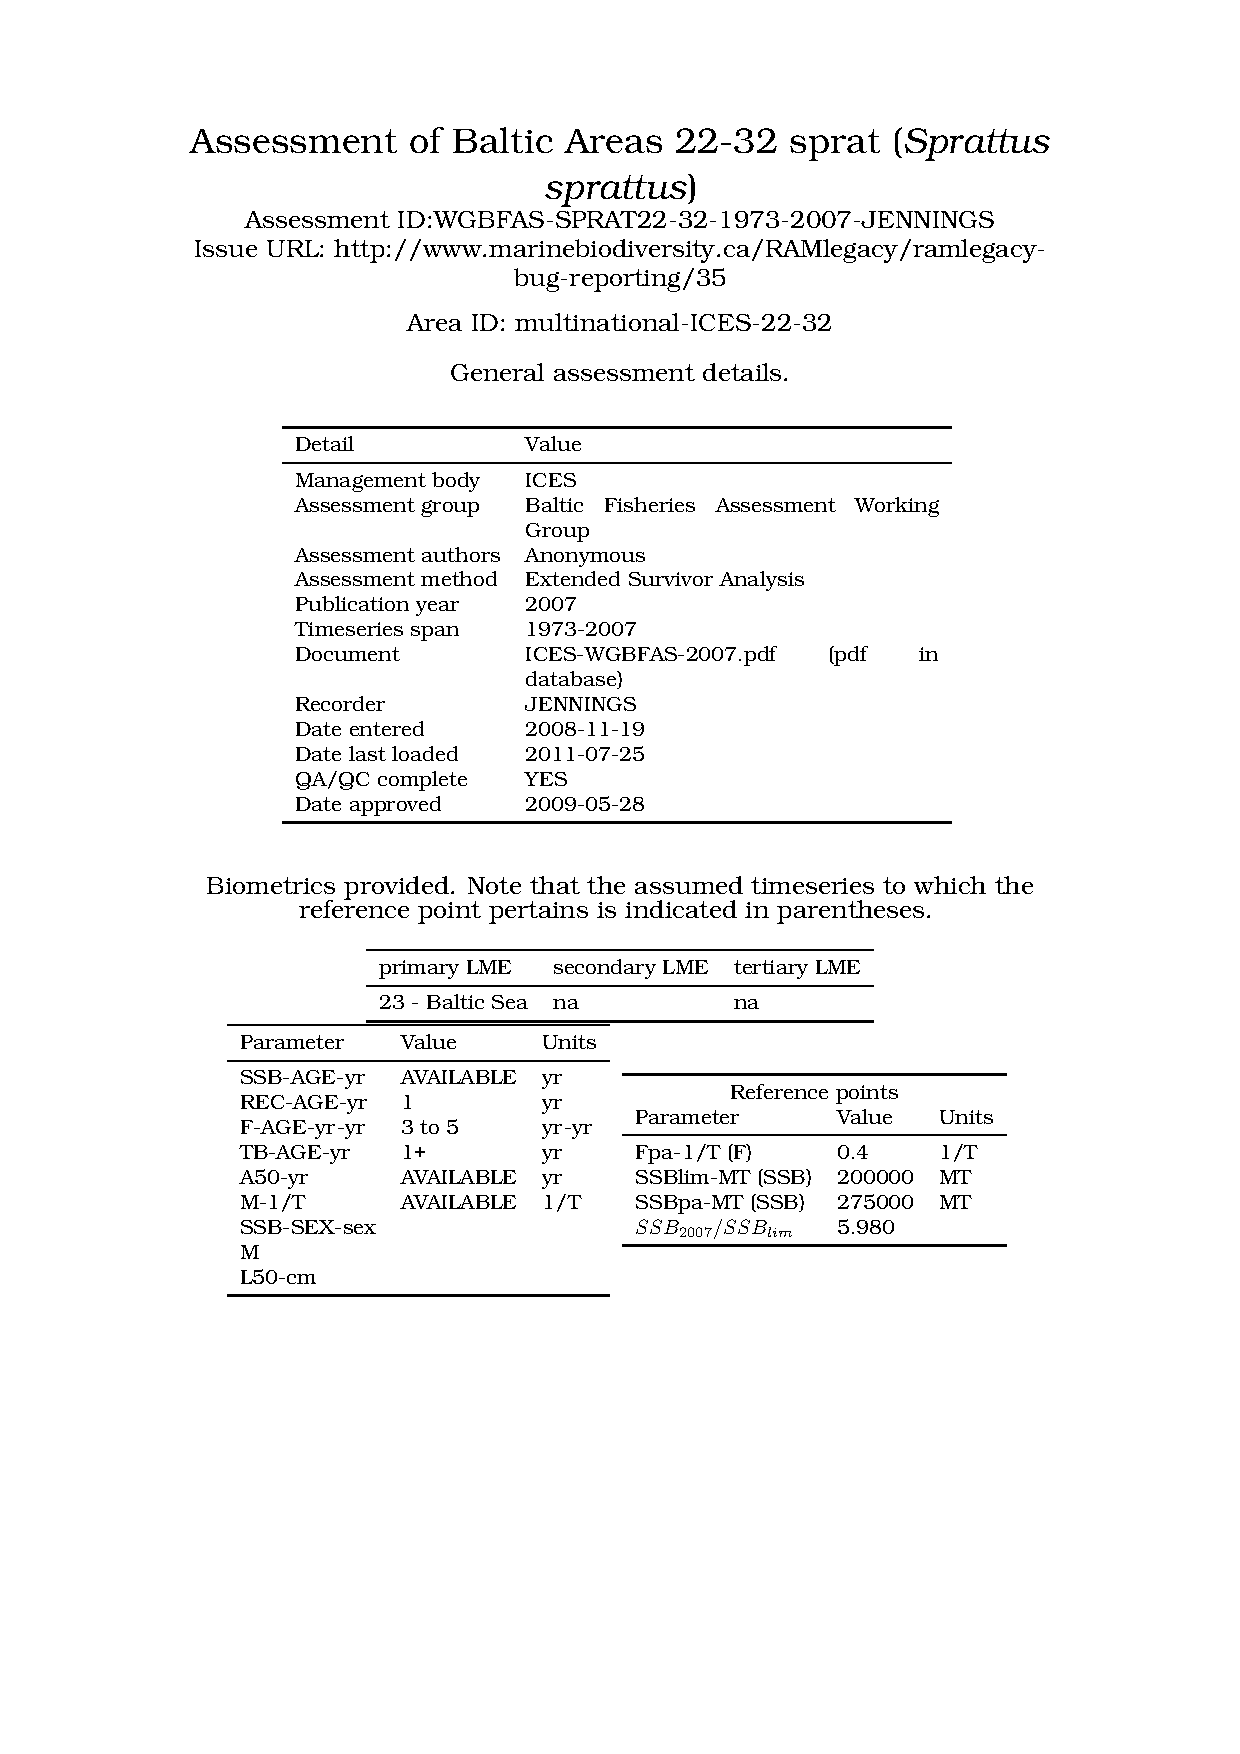
\includepdf[pagecommand={\thispagestyle{plain}}, pages={1,2}]{../../../tex/WGBFAS-SPRAT22-32-1973-2007-JENNINGS.pdf}
\index{Sprat}\index{Sprattus sprattus}\index{Clupeidae!Sprattus sprattus}
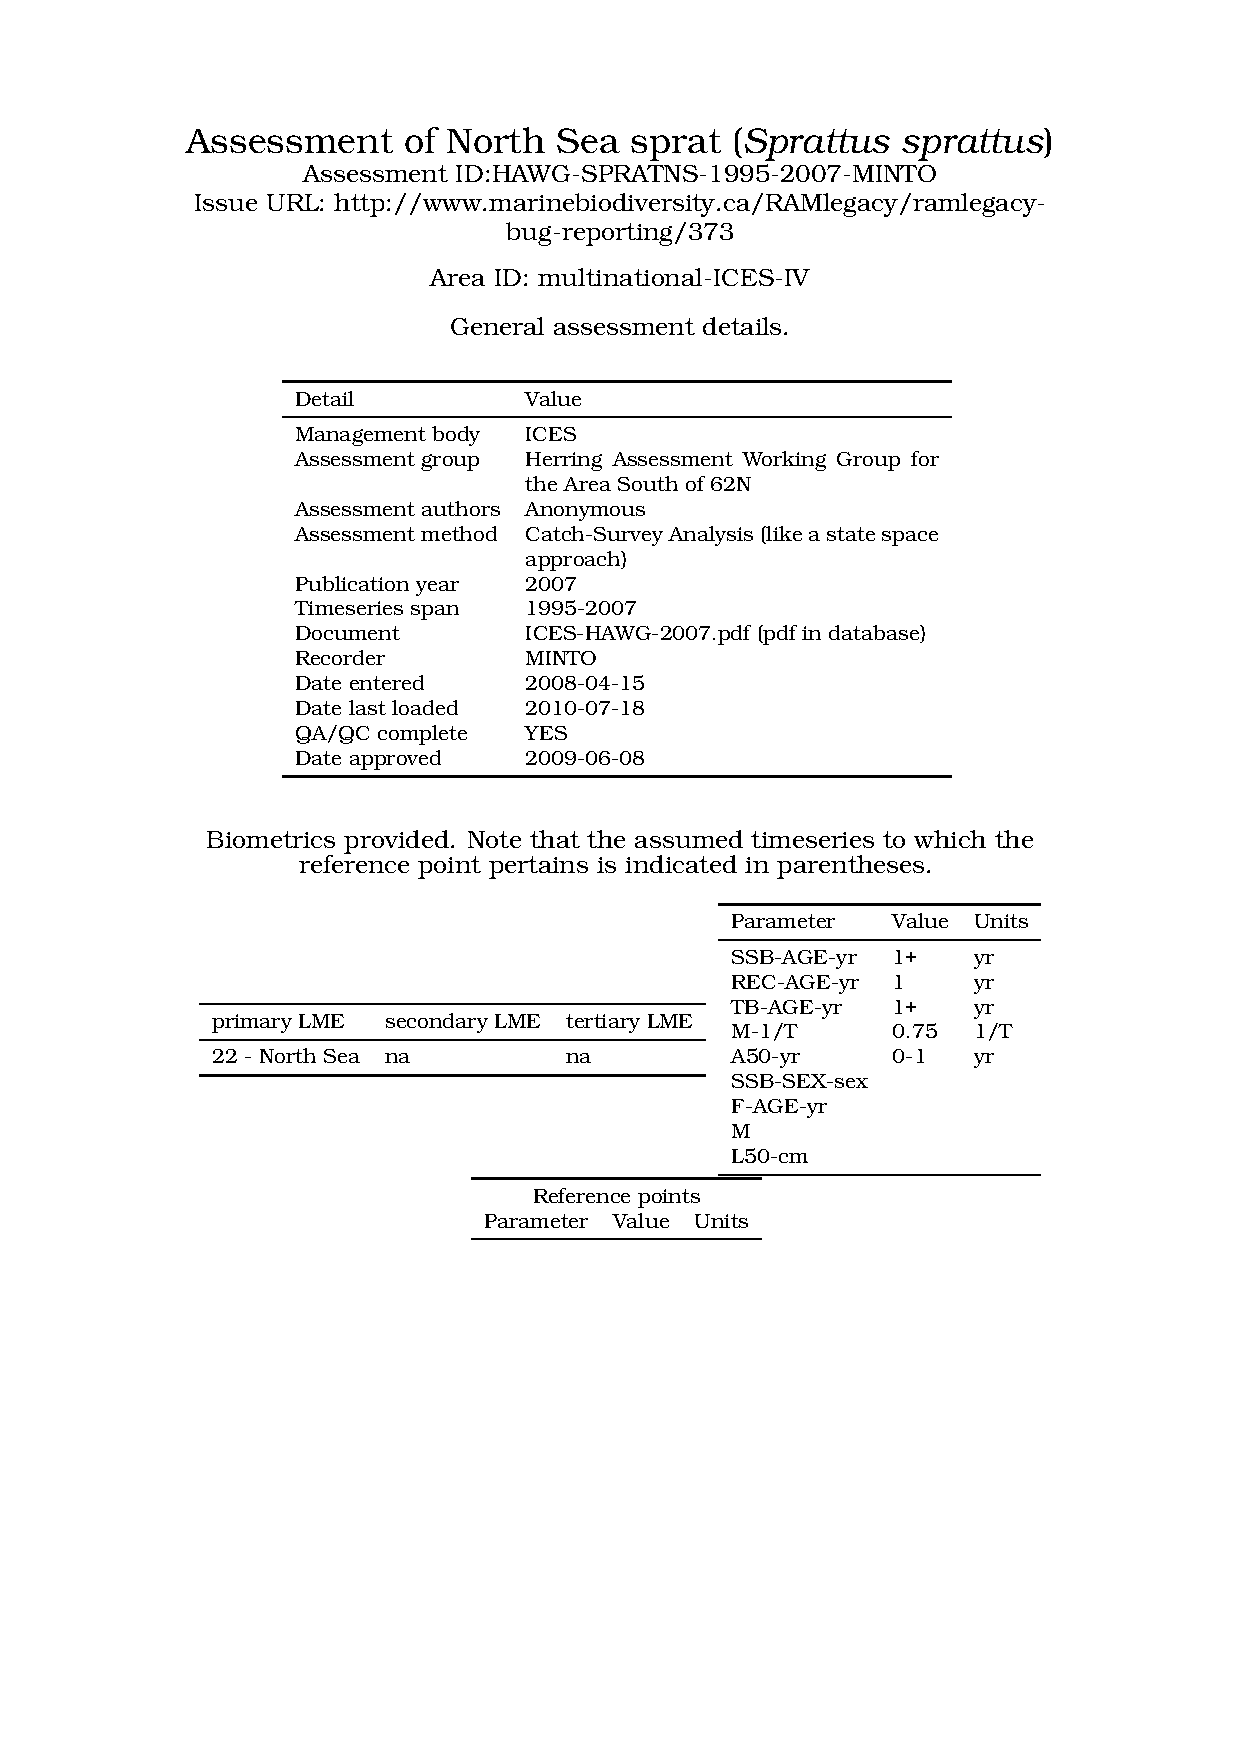
\includepdf[pagecommand={\thispagestyle{plain}}, pages={1,2}]{../../../tex/HAWG-SPRATNS-1995-2007-MINTO.pdf}
\index{Engraulidae}\index{Clupeiformes!Engraulidae}

\addcontentsline{toc}{subsection}{\hspace{0.2cm}Family Engraulidae}\index{Argentine anchoita}\index{Engraulis anchoita}\index{Engraulidae!Engraulis anchoita}
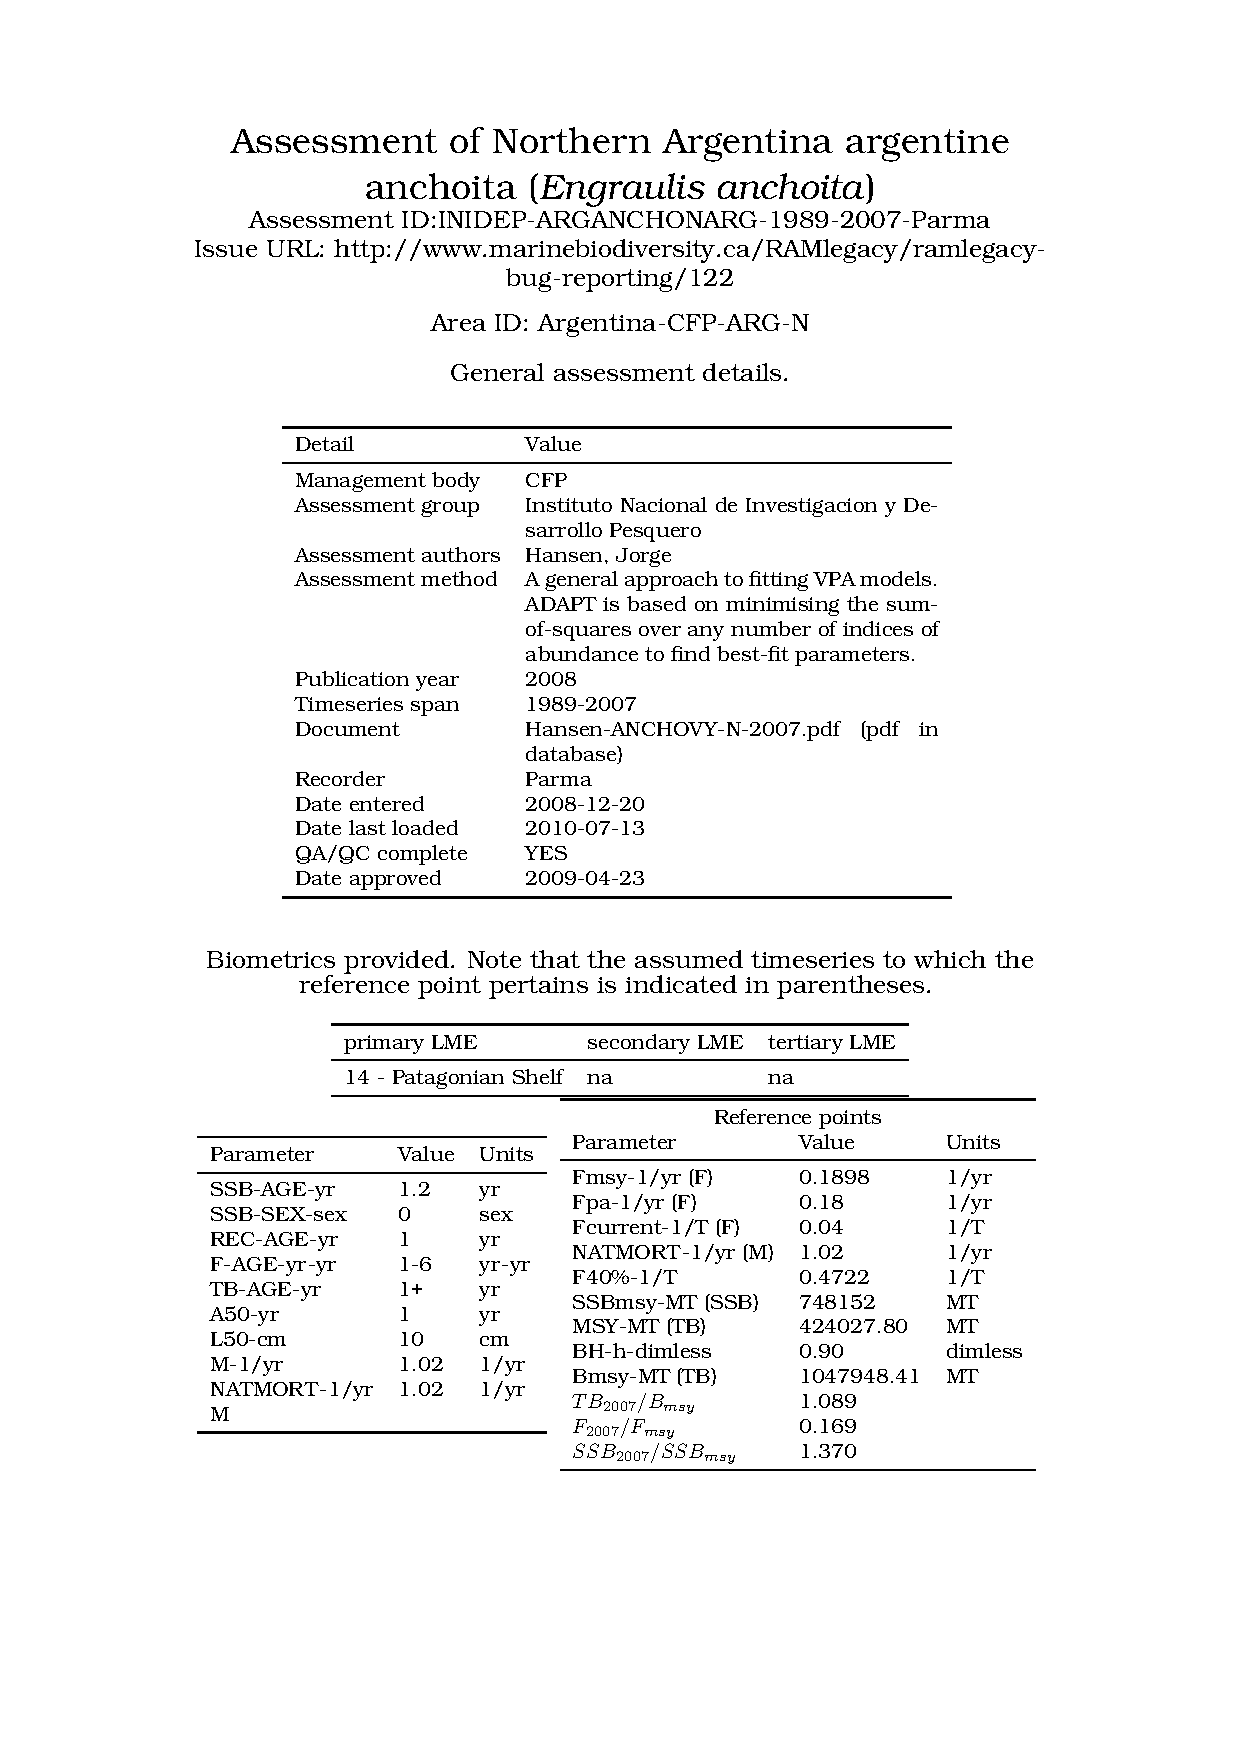
\includepdf[pagecommand={\thispagestyle{plain}}, pages={1,2}]{../../../tex/INIDEP-ARGANCHONARG-1989-2007-Parma.pdf}
\index{Argentine anchoita}\index{Engraulis anchoita}\index{Engraulidae!Engraulis anchoita}
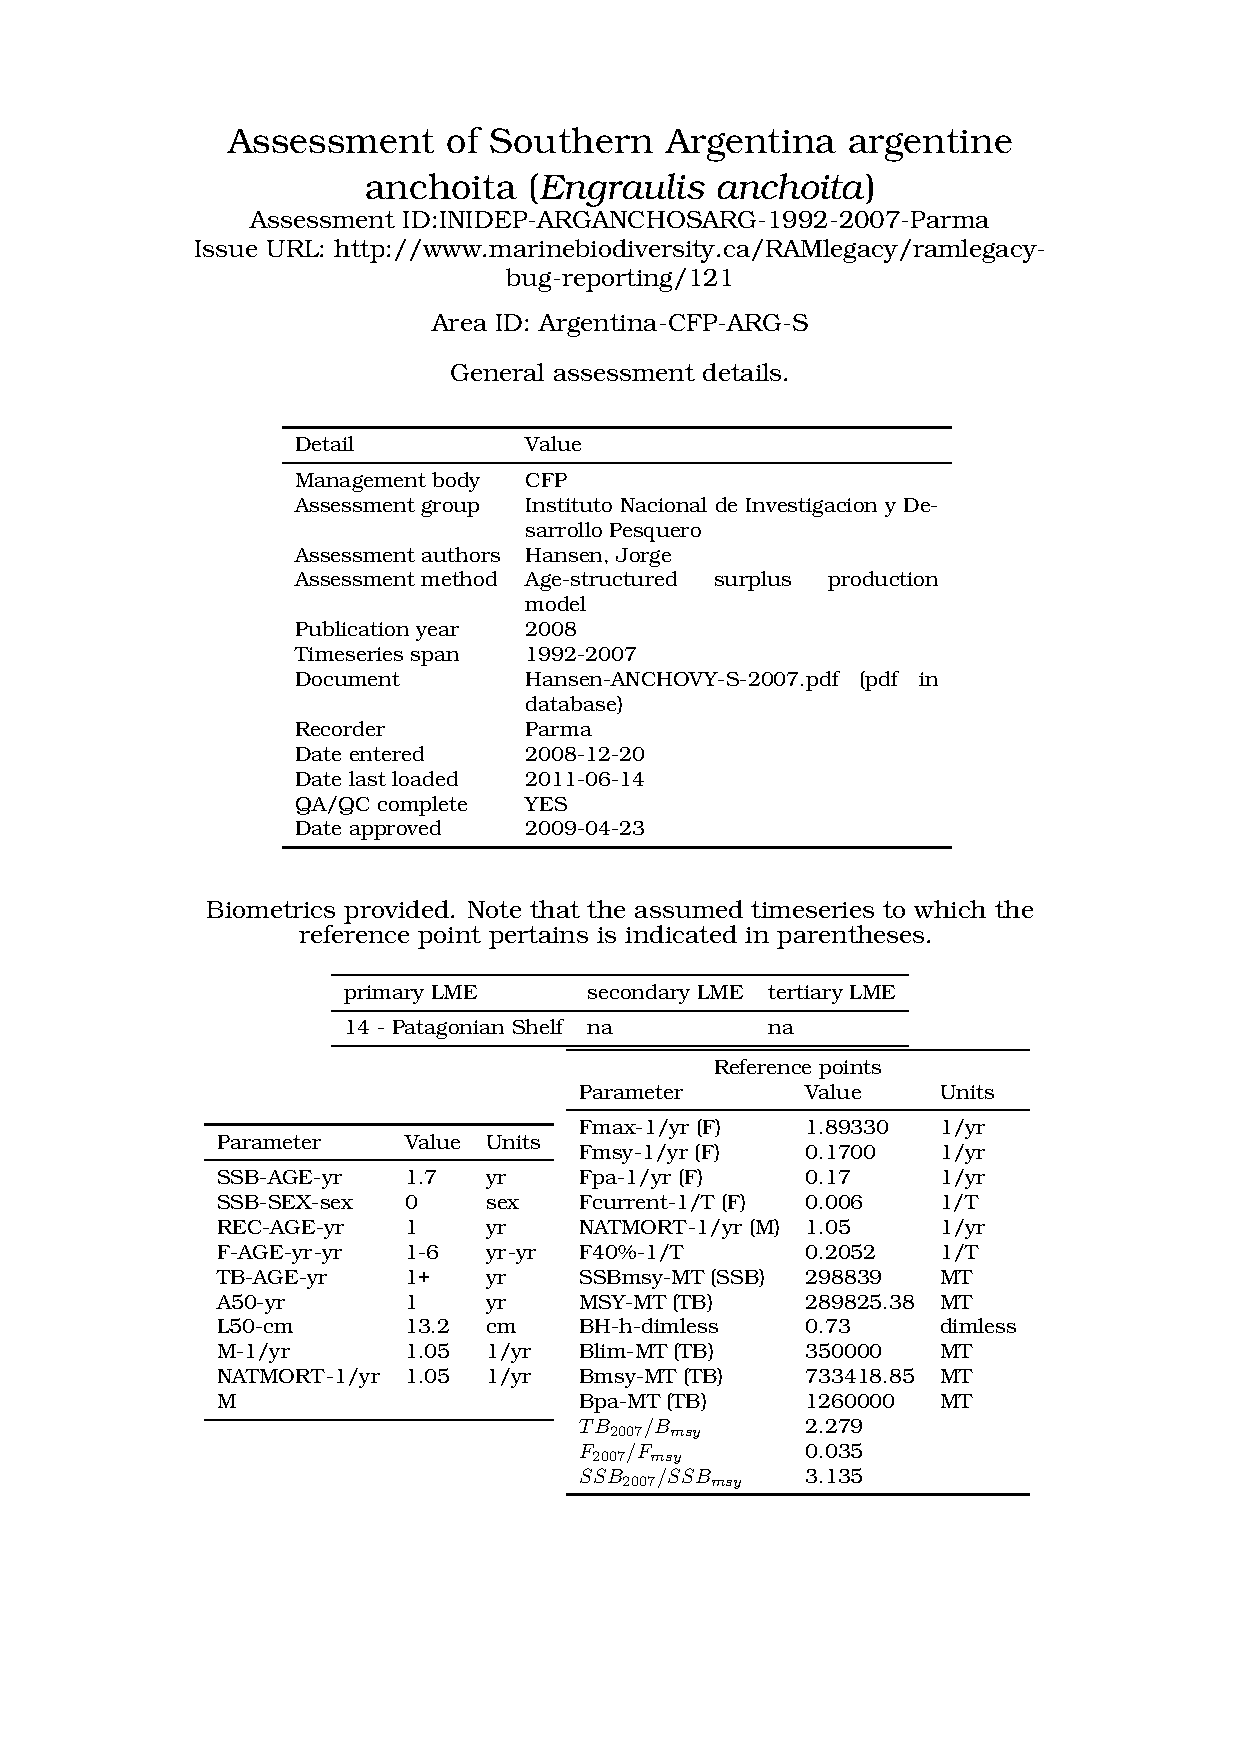
\includepdf[pagecommand={\thispagestyle{plain}}, pages={1,2}]{../../../tex/INIDEP-ARGANCHOSARG-1992-2007-Parma.pdf}
\index{Anchovy}\index{Engraulis encrasicolus}\index{Engraulidae!Engraulis encrasicolus}
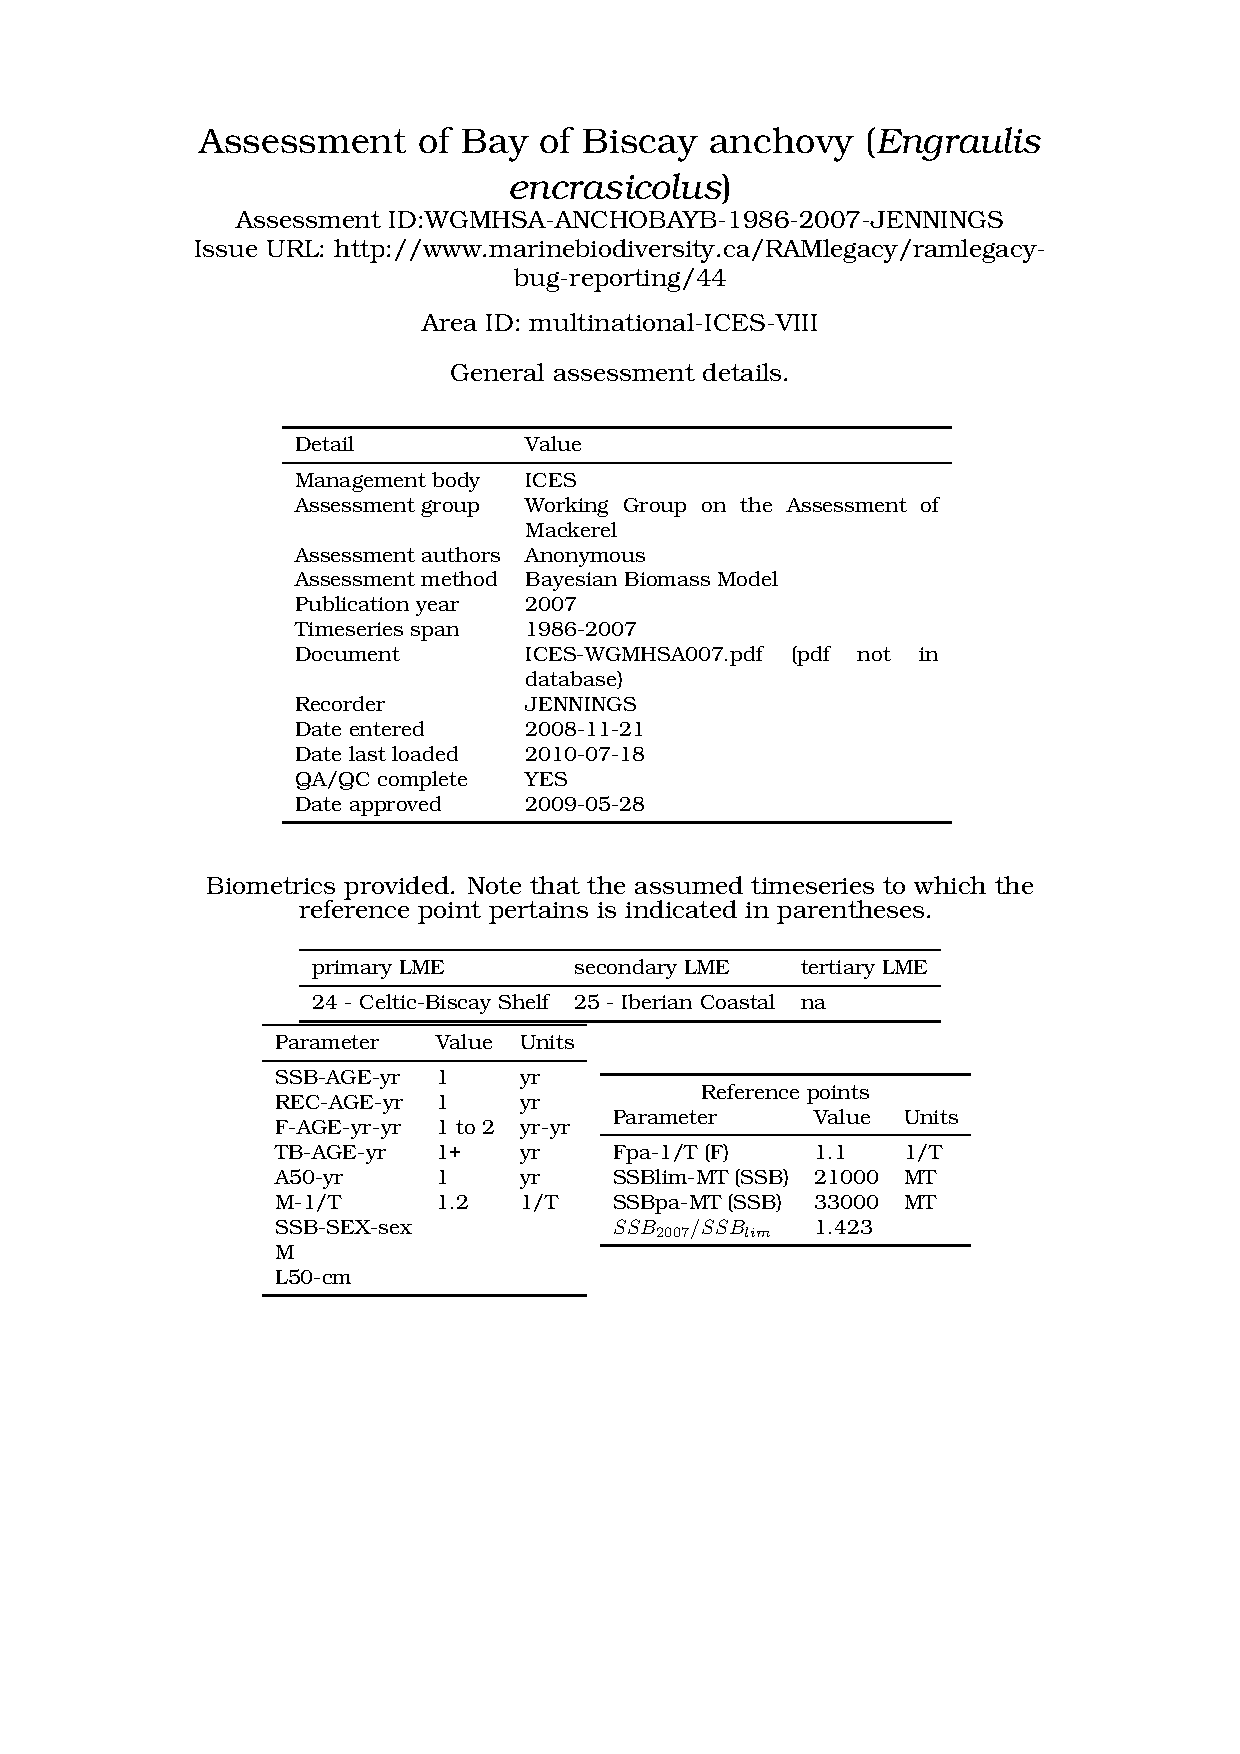
\includepdf[pagecommand={\thispagestyle{plain}}, pages={1,2}]{../../../tex/WGMHSA-ANCHOBAYB-1986-2007-JENNINGS.pdf}
\index{Anchovy}\index{Engraulis encrasicolus}\index{Engraulidae!Engraulis encrasicolus}
\includepdf[pagecommand={\thispagestyle{plain}}, pages={1,2}]{../../../tex/MARAM-ANCHOSA-1984-2006-deMoor.pdf}
\index{Peruvian anchoveta}\index{Engraulis ringens}\index{Engraulidae!Engraulis ringens}
\includepdf[pagecommand={\thispagestyle{plain}}, pages={1,2}]{../../../tex/IMARPE-PANCHPERUNC-1963-2004-RICARD.pdf}
\addcontentsline{toc}{section}{Order Decapoda}\index{Geryonidae}\index{Decapoda!Geryonidae}

\addcontentsline{toc}{subsection}{\hspace{0.2cm}Family Geryonidae}\index{Red deepsea crab}\index{Chaceon quinquedens}\index{Geryonidae!Chaceon quinquedens}
\includepdf[pagecommand={\thispagestyle{plain}}, pages={1,2}]{../../../tex/NEFSC-RDEEPCRABNWATL-1982-2008-CHUTE.pdf}
\index{Lithodidae}\index{Decapoda!Lithodidae}

\addcontentsline{toc}{subsection}{\hspace{0.2cm}Family Lithodidae}\index{Golden king crab}\index{Lithodes aequispinus}\index{Lithodidae!Lithodes aequispinus}
\includepdf[pagecommand={\thispagestyle{plain}}, pages={1,2}]{../../../tex/AFSC-GKINGCRABAIES-1990-2007-JENSEN.pdf}
\index{Golden king crab}\index{Lithodes aequispinus}\index{Lithodidae!Lithodes aequispinus}
\includepdf[pagecommand={\thispagestyle{plain}}, pages={1,2}]{../../../tex/AFSC-GKINGCRABAIWS-1989-2007-JENSEN.pdf}
\index{Red king crab}\index{Paralithodes camtschaticus}\index{Lithodidae!Paralithodes camtschaticus}
\includepdf[pagecommand={\thispagestyle{plain}}, pages={1,2}]{../../../tex/AFSC-RKCRABBB-1960-2008-JENSEN.pdf}
\index{Red king crab}\index{Paralithodes camtschaticus}\index{Lithodidae!Paralithodes camtschaticus}
\includepdf[pagecommand={\thispagestyle{plain}}, pages={1,2}]{../../../tex/AFSC-RKCRABNS-1976-2008-JENSEN.pdf}
\index{Red king crab}\index{Paralithodes camtschaticus}\index{Lithodidae!Paralithodes camtschaticus}
\includepdf[pagecommand={\thispagestyle{plain}}, pages={1,2}]{../../../tex/AFSC-RKCRABPI-1981-2009-JENSEN.pdf}
\index{Blue king crab}\index{Paralithodes platypus}\index{Lithodidae!Paralithodes platypus}
\includepdf[pagecommand={\thispagestyle{plain}}, pages={1,2}]{../../../tex/AFSC-BKINGCRABPI-1960-2008-JENSEN.pdf}
\index{Blue king crab}\index{Paralithodes platypus}\index{Lithodidae!Paralithodes platypus}
\includepdf[pagecommand={\thispagestyle{plain}}, pages={1,2}]{../../../tex/AFSC-BKINGCRABSMI-1960-2008-JENSEN.pdf}
\index{Menippidae}\index{Decapoda!Menippidae}

\addcontentsline{toc}{subsection}{\hspace{0.2cm}Family Menippidae}\index{Tasmanian giant crab}\index{Pseudocarcinus gigas}\index{Menippidae!Pseudocarcinus gigas}
\includepdf[pagecommand={\thispagestyle{plain}}, pages={1,2}]{../../../tex/TAFI-TASGIANTCRABTAS-1990-2007-JENSEN.pdf}
\index{Nephropidae}\index{Decapoda!Nephropidae}

\addcontentsline{toc}{subsection}{\hspace{0.2cm}Family Nephropidae}\index{American lobster}\index{Homarus americanus}\index{Nephropidae!Homarus americanus}
\includepdf[pagecommand={\thispagestyle{plain}}, pages={1,2}]{../../../tex/RIDEM-LOBSTERRI-1959-2007-COLLIE.pdf}
\index{American lobster}\index{Homarus americanus}\index{Nephropidae!Homarus americanus}
\includepdf[pagecommand={\thispagestyle{plain}}, pages={1,2}]{../../../tex/ASMFC-LOBSTERGB-1981-2007-STANTON.pdf}
\index{American lobster}\index{Homarus americanus}\index{Nephropidae!Homarus americanus}
\includepdf[pagecommand={\thispagestyle{plain}}, pages={1,2}]{../../../tex/ASMFC-LOBSTERGOM-1981-2007-STANTON.pdf}
\index{American lobster}\index{Homarus americanus}\index{Nephropidae!Homarus americanus}
\includepdf[pagecommand={\thispagestyle{plain}}, pages={1,2}]{../../../tex/ASMFC-LOBSTERSNE-1981-2007-STANTON.pdf}
\index{Oregoniidae}\index{Decapoda!Oregoniidae}

\addcontentsline{toc}{subsection}{\hspace{0.2cm}Family Oregoniidae}\index{Tanner crab}\index{Chionoecetes bairdi}\index{Oregoniidae!Chionoecetes bairdi}
\includepdf[pagecommand={\thispagestyle{plain}}, pages={1,2}]{../../../tex/AFSC-TANNERCRABBSAI-1965-2008-JENSEN.pdf}
\index{Snow crab}\index{Chionoecetes opilio}\index{Oregoniidae!Chionoecetes opilio}
\includepdf[pagecommand={\thispagestyle{plain}}, pages={1,2}]{../../../tex/DFO-SG-SNOWCRABSGSL-1984-2007-ANDERSON.pdf}
\index{Snow crab}\index{Chionoecetes opilio}\index{Oregoniidae!Chionoecetes opilio}
\includepdf[pagecommand={\thispagestyle{plain}}, pages={1,2}]{../../../tex/AFSC-SNOWCRABBS-1979-2008-JENSEN.pdf}
\index{Palinuridae}\index{Decapoda!Palinuridae}

\addcontentsline{toc}{subsection}{\hspace{0.2cm}Family Palinuridae}\index{Red rock lobster}\index{Jasus edwardsii}\index{Palinuridae!Jasus edwardsii}
\includepdf[pagecommand={\thispagestyle{plain}}, pages={1,2}]{../../../tex/NZMFishLOBSTERWG-RROCKLOBSTERCRA1-1945-2001-JENSEN.pdf}
\index{Red rock lobster}\index{Jasus edwardsii}\index{Palinuridae!Jasus edwardsii}
\includepdf[pagecommand={\thispagestyle{plain}}, pages={1,2}]{../../../tex/NZMFishLOBSTERWG-RROCKLOBSTERCRA2-1945-2001-JENSEN.pdf}
\index{Red rock lobster}\index{Jasus edwardsii}\index{Palinuridae!Jasus edwardsii}
\includepdf[pagecommand={\thispagestyle{plain}}, pages={1,2}]{../../../tex/NZMFishLOBSTERWG-RROCKLOBSTERCRA3-1945-2007-JENSEN.pdf}
\index{Red rock lobster}\index{Jasus edwardsii}\index{Palinuridae!Jasus edwardsii}
\includepdf[pagecommand={\thispagestyle{plain}}, pages={1,2}]{../../../tex/NZMFishLOBSTERWG-RROCKLOBSTERCRA4-1945-2005-JENSEN.pdf}
\index{Red rock lobster}\index{Jasus edwardsii}\index{Palinuridae!Jasus edwardsii}
\includepdf[pagecommand={\thispagestyle{plain}}, pages={1,2}]{../../../tex/NZMFishLOBSTERWG-RROCKLOBSTERCRA5-1945-2002-JENSEN.pdf}
\index{Red rock lobster}\index{Jasus edwardsii}\index{Palinuridae!Jasus edwardsii}
\includepdf[pagecommand={\thispagestyle{plain}}, pages={1,2}]{../../../tex/NZMFishLOBSTERWG-RROCKLOBSTERCRA7-1976-2005-JENSEN.pdf}
\index{Red rock lobster}\index{Jasus edwardsii}\index{Palinuridae!Jasus edwardsii}
\includepdf[pagecommand={\thispagestyle{plain}}, pages={1,2}]{../../../tex/NZMFishLOBSTERWG-RROCKLOBSTERCRA8-1976-2005-JENSEN.pdf}
\index{South African west coast rock lobster}\index{Jasus lalandii}\index{Palinuridae!Jasus lalandii}
\includepdf[pagecommand={\thispagestyle{plain}}, pages={1,2}]{../../../tex/MARAM-CRLOBSTERSA7-1910-2008-Johnston.pdf}
\index{South African west coast rock lobster}\index{Jasus lalandii}\index{Palinuridae!Jasus lalandii}
\includepdf[pagecommand={\thispagestyle{plain}}, pages={1,2}]{../../../tex/MARAM-CRLOBSTERSA8-1910-2008-Johnston.pdf}
\index{South African west coast rock lobster}\index{Jasus lalandii}\index{Palinuridae!Jasus lalandii}
\includepdf[pagecommand={\thispagestyle{plain}}, pages={1,2}]{../../../tex/MARAM-CRLOBSTERSA12-1910-2008-Johnston.pdf}
\index{South African west coast rock lobster}\index{Jasus lalandii}\index{Palinuridae!Jasus lalandii}
\includepdf[pagecommand={\thispagestyle{plain}}, pages={1,2}]{../../../tex/MARAM-CRLOBSTERSA34-1910-2008-Johnston.pdf}
\index{South African west coast rock lobster}\index{Jasus lalandii}\index{Palinuridae!Jasus lalandii}
\includepdf[pagecommand={\thispagestyle{plain}}, pages={1,2}]{../../../tex/MARAM-CRLOBSTERSA56-1910-2008-Johnston.pdf}
\index{Southern spiny lobster}\index{Palinurus gilchristi}\index{Palinuridae!Palinurus gilchristi}
\includepdf[pagecommand={\thispagestyle{plain}}, pages={1,2}]{../../../tex/MARAM-SSLOBSTERSASC-1973-2008-Johnston.pdf}
\index{Pandalidae}\index{Decapoda!Pandalidae}

\addcontentsline{toc}{subsection}{\hspace{0.2cm}Family Pandalidae}\index{Northern shrimp}\index{Pandalus borealis}\index{Pandalidae!Pandalus borealis}
\includepdf[pagecommand={\thispagestyle{plain}}, pages={1,2}]{../../../tex/ASMFC-PANDALGOM-1960-2009-IDOINE.pdf}
\index{Penaeidae}\index{Decapoda!Penaeidae}

\addcontentsline{toc}{subsection}{\hspace{0.2cm}Family Penaeidae}\index{Brown tiger shrimp}\index{Penaeus esculentus}\index{Penaeidae!Penaeus esculentus}
\includepdf[pagecommand={\thispagestyle{plain}}, pages={1,2}]{../../../tex/CSIRO-BTSHRIMPNAUST-1970-2006-FULTON.pdf}
\index{Brown tiger shrimp}\index{Penaeus esculentus}\index{Penaeidae!Penaeus esculentus}
\includepdf[pagecommand={\thispagestyle{plain}}, pages={1,2}]{../../../tex/CSIRO-GTPRAWNNAUST-1970-2006-FULTON.pdf}
\addcontentsline{toc}{section}{Order Gadiformes}\index{Gadidae}\index{Gadiformes!Gadidae}

\addcontentsline{toc}{subsection}{\hspace{0.2cm}Family Gadidae}\index{Pacific cod}\index{Gadus macrocephalus}\index{Gadidae!Gadus macrocephalus}
\includepdf[pagecommand={\thispagestyle{plain}}, pages={1,2}]{../../../tex/DFO-PAC-PCODHS-1956-2005-COLLIE.pdf}
\index{Pacific cod}\index{Gadus macrocephalus}\index{Gadidae!Gadus macrocephalus}
\includepdf[pagecommand={\thispagestyle{plain}}, pages={1,2}]{../../../tex/DFO-PAC-PCODWCVANI-1956-2002-COLLIE.pdf}
\index{Pacific cod}\index{Gadus macrocephalus}\index{Gadidae!Gadus macrocephalus}
\includepdf[pagecommand={\thispagestyle{plain}}, pages={1,2}]{../../../tex/AFSC-PCODBSAI-1964-2008-MELNYCHUK.pdf}
\index{Pacific cod}\index{Gadus macrocephalus}\index{Gadidae!Gadus macrocephalus}
\includepdf[pagecommand={\thispagestyle{plain}}, pages={1,2}]{../../../tex/AFSC-PCODGA-1964-2008-MELNYCHUK.pdf}
\index{Atlantic cod}\index{Gadus morhua}\index{Gadidae!Gadus morhua}
\includepdf[pagecommand={\thispagestyle{plain}}, pages={1,2}]{../../../tex/NEFSC-CODGB-1960-2008-BAUM.pdf}
\index{Atlantic cod}\index{Gadus morhua}\index{Gadidae!Gadus morhua}
\includepdf[pagecommand={\thispagestyle{plain}}, pages={1,2}]{../../../tex/NEFSC-CODGOM-1893-2008-BAUM.pdf}
\index{Atlantic cod}\index{Gadus morhua}\index{Gadidae!Gadus morhua}
\includepdf[pagecommand={\thispagestyle{plain}}, pages={1,2}]{../../../tex/NAFO-SC-COD3M-1959-2008-BAUM.pdf}
\index{Atlantic cod}\index{Gadus morhua}\index{Gadidae!Gadus morhua}
\includepdf[pagecommand={\thispagestyle{plain}}, pages={1,2}]{../../../tex/NAFO-SC-COD3NO-1953-2007-BAUM.pdf}
\index{Atlantic cod}\index{Gadus morhua}\index{Gadidae!Gadus morhua}
\includepdf[pagecommand={\thispagestyle{plain}}, pages={1,2}]{../../../tex/WGBFAS-CODBA2224-1969-2007-JENNINGS.pdf}
\index{Atlantic cod}\index{Gadus morhua}\index{Gadidae!Gadus morhua}
\includepdf[pagecommand={\thispagestyle{plain}}, pages={1,2}]{../../../tex/WGBFAS-CODBA2532-1964-2007-JENNINGS.pdf}
\index{Atlantic cod}\index{Gadus morhua}\index{Gadidae!Gadus morhua}
\includepdf[pagecommand={\thispagestyle{plain}}, pages={1,2}]{../../../tex/NWWG-CODFAPL-1959-2006-MINTO.pdf}
\index{Atlantic cod}\index{Gadus morhua}\index{Gadidae!Gadus morhua}
\includepdf[pagecommand={\thispagestyle{plain}}, pages={1,2}]{../../../tex/NWWG-CODICE-1952-2006-MINTO.pdf}
\index{Atlantic cod}\index{Gadus morhua}\index{Gadidae!Gadus morhua}
\includepdf[pagecommand={\thispagestyle{plain}}, pages={1,2}]{../../../tex/WGNSDS-CODIS-1968-2006-MINTO.pdf}
\index{Atlantic cod}\index{Gadus morhua}\index{Gadidae!Gadus morhua}
\includepdf[pagecommand={\thispagestyle{plain}}, pages={1,2}]{../../../tex/WGBFAS-CODKAT-1970-2006-MINTO.pdf}
\index{Atlantic cod}\index{Gadus morhua}\index{Gadidae!Gadus morhua}
\includepdf[pagecommand={\thispagestyle{plain}}, pages={1,2}]{../../../tex/WGNSSK-CODNS-1962-2007-MINTO.pdf}
\index{Atlantic cod}\index{Gadus morhua}\index{Gadidae!Gadus morhua}
\includepdf[pagecommand={\thispagestyle{plain}}, pages={1,2}]{../../../tex/AFWG-CODNEAR-1943-2006-MINTO.pdf}
\index{Atlantic cod}\index{Gadus morhua}\index{Gadidae!Gadus morhua}
\includepdf[pagecommand={\thispagestyle{plain}}, pages={1,2}]{../../../tex/WGNSDS-CODVIa-1977-2006-MINTO.pdf}
\index{Atlantic cod}\index{Gadus morhua}\index{Gadidae!Gadus morhua}
\includepdf[pagecommand={\thispagestyle{plain}}, pages={1,2}]{../../../tex/AFWG-CODCOASTNOR-1982-2006-MINTO.pdf}
\index{Atlantic cod}\index{Gadus morhua}\index{Gadidae!Gadus morhua}
\includepdf[pagecommand={\thispagestyle{plain}}, pages={1,2}]{../../../tex/DFO-NFLD-COD2J3KLIS-1959-2006-PREFONTAINE.pdf}
\index{Atlantic cod}\index{Gadus morhua}\index{Gadidae!Gadus morhua}
\includepdf[pagecommand={\thispagestyle{plain}}, pages={1,2}]{../../../tex/DFO-QUE-COD3Pn4RS-1964-2007-PREFONTAINE.pdf}
\index{Atlantic cod}\index{Gadus morhua}\index{Gadidae!Gadus morhua}
\includepdf[pagecommand={\thispagestyle{plain}}, pages={1,2}]{../../../tex/DFO-NFLD-COD3Ps-1959-2004-PREFONTAINE.pdf}
\index{Atlantic cod}\index{Gadus morhua}\index{Gadidae!Gadus morhua}
\includepdf[pagecommand={\thispagestyle{plain}}, pages={1,2}]{../../../tex/DFO-SG-COD4TVn-1965-2007-PREFONTAINE.pdf}
\index{Atlantic cod}\index{Gadus morhua}\index{Gadidae!Gadus morhua}
\includepdf[pagecommand={\thispagestyle{plain}}, pages={1,2}]{../../../tex/DFO-MAR-COD4VsW-1958-2002-PREFONTAINE.pdf}
\index{Atlantic cod}\index{Gadus morhua}\index{Gadidae!Gadus morhua}
\includepdf[pagecommand={\thispagestyle{plain}}, pages={1,2}]{../../../tex/DFO-COD5Zjm-1978-2003-PREFONTAINE.pdf}
\index{Haddock}\index{Melanogrammus aeglefinus}\index{Gadidae!Melanogrammus aeglefinus}
\includepdf[pagecommand={\thispagestyle{plain}}, pages={1,2}]{../../../tex/NEFSC-HADGB-1930-2008-BAUM.pdf}
\index{Haddock}\index{Melanogrammus aeglefinus}\index{Gadidae!Melanogrammus aeglefinus}
\includepdf[pagecommand={\thispagestyle{plain}}, pages={1,2}]{../../../tex/NEFSC-HAD5Y-1956-2008-BAUM.pdf}
\index{Haddock}\index{Melanogrammus aeglefinus}\index{Gadidae!Melanogrammus aeglefinus}
\includepdf[pagecommand={\thispagestyle{plain}}, pages={1,2}]{../../../tex/WGSSDS-HADVIIb-k-1993-2006-JENNINGS.pdf}
\index{Haddock}\index{Melanogrammus aeglefinus}\index{Gadidae!Melanogrammus aeglefinus}
\includepdf[pagecommand={\thispagestyle{plain}}, pages={1,2}]{../../../tex/WGNSSK-HADROCK-1990-2007-JENNINGS.pdf}
\index{Haddock}\index{Melanogrammus aeglefinus}\index{Gadidae!Melanogrammus aeglefinus}
\includepdf[pagecommand={\thispagestyle{plain}}, pages={1,2}]{../../../tex/NWWG-HADFAPL-1955-2006-MINTO.pdf}
\index{Haddock}\index{Melanogrammus aeglefinus}\index{Gadidae!Melanogrammus aeglefinus}
\includepdf[pagecommand={\thispagestyle{plain}}, pages={1,2}]{../../../tex/WGNSSK-HADNS-IIIa-1963-2006-MINTO.pdf}
\index{Haddock}\index{Melanogrammus aeglefinus}\index{Gadidae!Melanogrammus aeglefinus}
\includepdf[pagecommand={\thispagestyle{plain}}, pages={1,2}]{../../../tex/NWWG-HADICE-1977-2007-MINTO.pdf}
\index{Haddock}\index{Melanogrammus aeglefinus}\index{Gadidae!Melanogrammus aeglefinus}
\includepdf[pagecommand={\thispagestyle{plain}}, pages={1,2}]{../../../tex/WGNSDS-HADIS-1972-2006-MINTO.pdf}
\index{Haddock}\index{Melanogrammus aeglefinus}\index{Gadidae!Melanogrammus aeglefinus}
\includepdf[pagecommand={\thispagestyle{plain}}, pages={1,2}]{../../../tex/AFWG-HADNEAR-1947-2006-MINTO.pdf}
\index{Haddock}\index{Melanogrammus aeglefinus}\index{Gadidae!Melanogrammus aeglefinus}
\includepdf[pagecommand={\thispagestyle{plain}}, pages={1,2}]{../../../tex/WGNSDS-HADVIa-1977-2006-MINTO.pdf}
\index{Haddock}\index{Melanogrammus aeglefinus}\index{Gadidae!Melanogrammus aeglefinus}
\includepdf[pagecommand={\thispagestyle{plain}}, pages={1,2}]{../../../tex/DFO-HAD4X5Y-1960-2003-PREFONTAINE.pdf}
\index{Haddock}\index{Melanogrammus aeglefinus}\index{Gadidae!Melanogrammus aeglefinus}
\includepdf[pagecommand={\thispagestyle{plain}}, pages={1,2}]{../../../tex/DFO-HAD5Zejm-1968-2003-PREFONTAINE.pdf}
\index{Whiting}\index{Merlangius merlangus}\index{Gadidae!Merlangius merlangus}
\includepdf[pagecommand={\thispagestyle{plain}}, pages={1,2}]{../../../tex/WGSSDS-WHITVIIek-1982-2007-JENNINGS.pdf}
\index{Whiting}\index{Merlangius merlangus}\index{Gadidae!Merlangius merlangus}
\includepdf[pagecommand={\thispagestyle{plain}}, pages={1,2}]{../../../tex/WGNSSK-WHITNS-VIId-IIIa-1979-2006-MINTO.pdf}
\index{Whiting}\index{Merlangius merlangus}\index{Gadidae!Merlangius merlangus}
\includepdf[pagecommand={\thispagestyle{plain}}, pages={1,2}]{../../../tex/WGNSDS-WHITVIa-1984-2007-MINTO.pdf}
\index{Southern blue whiting}\index{Micromesistius australis}\index{Gadidae!Micromesistius australis}
\includepdf[pagecommand={\thispagestyle{plain}}, pages={1,2}]{../../../tex/NZMFishMIDDEPTHSWG-SBWHITACIR-1979-2006-JENSEN.pdf}
\index{Southern blue whiting}\index{Micromesistius australis}\index{Gadidae!Micromesistius australis}
\includepdf[pagecommand={\thispagestyle{plain}}, pages={1,2}]{../../../tex/INIDEP-SBWHITARGS-1985-2007-Parma.pdf}
\index{Blue whiting}\index{Micromesistius poutassou}\index{Gadidae!Micromesistius poutassou}
\includepdf[pagecommand={\thispagestyle{plain}}, pages={1,2}]{../../../tex/WGNPBW-BWHITNEA-1980-2007-JENNINGS.pdf}
\index{Pollock}\index{Pollachius virens}\index{Gadidae!Pollachius virens}
\includepdf[pagecommand={\thispagestyle{plain}}, pages={1,2}]{../../../tex/NEFSC-POLL5YZ-1963-2007-MAYO.pdf}
\index{Pollock}\index{Pollachius virens}\index{Gadidae!Pollachius virens}
\includepdf[pagecommand={\thispagestyle{plain}}, pages={1,2}]{../../../tex/NWWG-POLLFAPL-1958-2006-MINTO.pdf}
\index{Pollock}\index{Pollachius virens}\index{Gadidae!Pollachius virens}
\includepdf[pagecommand={\thispagestyle{plain}}, pages={1,2}]{../../../tex/WGNSSK-POLLNS-VI-IIIa-1964-2006-MINTO.pdf}
\index{Pollock}\index{Pollachius virens}\index{Gadidae!Pollachius virens}
\includepdf[pagecommand={\thispagestyle{plain}}, pages={1,2}]{../../../tex/AFWG-POLLNEAR-1957-2006-MINTO.pdf}
\index{Pollock}\index{Pollachius virens}\index{Gadidae!Pollachius virens}
\includepdf[pagecommand={\thispagestyle{plain}}, pages={1,2}]{../../../tex/DFO-POLL4VWX5Zc-1974-2007-PREFONTAINE.pdf}
\index{Walleye pollock}\index{Theragra chalcogramma}\index{Gadidae!Theragra chalcogramma}
\includepdf[pagecommand={\thispagestyle{plain}}, pages={1,2}]{../../../tex/SFI-WPOLLNSO-1985-1994-JENSEN.pdf}
\index{Walleye pollock}\index{Theragra chalcogramma}\index{Gadidae!Theragra chalcogramma}
\includepdf[pagecommand={\thispagestyle{plain}}, pages={1,2}]{../../../tex/VNIRO-WPOLLWBS-1994-2004-JENSEN.pdf}
\index{Walleye pollock}\index{Theragra chalcogramma}\index{Gadidae!Theragra chalcogramma}
\includepdf[pagecommand={\thispagestyle{plain}}, pages={1,2}]{../../../tex/AFSC-WPOLLAI-1976-2008-MELNYCHUK.pdf}
\index{Walleye pollock}\index{Theragra chalcogramma}\index{Gadidae!Theragra chalcogramma}
\includepdf[pagecommand={\thispagestyle{plain}}, pages={1,2}]{../../../tex/AFSC-WPOLLEBS-1963-2008-MELNYCHUK.pdf}
\index{Walleye pollock}\index{Theragra chalcogramma}\index{Gadidae!Theragra chalcogramma}
\includepdf[pagecommand={\thispagestyle{plain}}, pages={1,2}]{../../../tex/AFSC-WPOLLGA-1964-2008-MELNYCHUK.pdf}
\index{Norway Pout}\index{Trisopterus esmarkii}\index{Gadidae!Trisopterus esmarkii}
\includepdf[pagecommand={\thispagestyle{plain}}, pages={1,2}]{../../../tex/WGNSSK-NPOUTNS-1983-2007-MINTO.pdf}
\index{White hake}\index{Urophycis tenuis}\index{Gadidae!Urophycis tenuis}
\includepdf[pagecommand={\thispagestyle{plain}}, pages={1,2}]{../../../tex/DFO-MAR-WHAKE4VWX5-1964-2005-PREFONTAINE.pdf}
\index{White hake}\index{Urophycis tenuis}\index{Gadidae!Urophycis tenuis}
\includepdf[pagecommand={\thispagestyle{plain}}, pages={1,2}]{../../../tex/NEFSC-WHAKEGBGOM-1963-2007-SOSEBEE.pdf}
\index{Merlucciidae}\index{Gadiformes!Merlucciidae}

\addcontentsline{toc}{subsection}{\hspace{0.2cm}Family Merlucciidae}\index{Patagonian grenadier}\index{Macruronus magellanicus}\index{Merlucciidae!Macruronus magellanicus}
\includepdf[pagecommand={\thispagestyle{plain}}, pages={1,2}]{../../../tex/INIDEP-PATGRENADIERSARG-1983-2006-Parma.pdf}
\index{Hoki}\index{Macruronus novaezelandiae}\index{Merlucciidae!Macruronus novaezelandiae}
\includepdf[pagecommand={\thispagestyle{plain}}, pages={1,2}]{../../../tex/NZMFishHOKIWG-HOKIENZ-1972-2007-FRANCIS.pdf}
\index{Hoki}\index{Macruronus novaezelandiae}\index{Merlucciidae!Macruronus novaezelandiae}
\includepdf[pagecommand={\thispagestyle{plain}}, pages={1,2}]{../../../tex/NZMFishHOKIWG-HOKIWNZ-1972-2007-FRANCIS.pdf}
\index{Silver Hake}\index{Merluccius bilinearis}\index{Merlucciidae!Merluccius bilinearis}
\includepdf[pagecommand={\thispagestyle{plain}}, pages={1,2}]{../../../tex/NEFSC-SHAKEGOMNGB-1955-2005-COL.pdf}
\index{Silver Hake}\index{Merluccius bilinearis}\index{Merlucciidae!Merluccius bilinearis}
\includepdf[pagecommand={\thispagestyle{plain}}, pages={1,2}]{../../../tex/NEFSC-SHAKESGBMATL-1955-2005-COL.pdf}
\index{Shallow-water cape hake}\index{Merluccius capensis}\index{Merlucciidae!Merluccius capensis}
\includepdf[pagecommand={\thispagestyle{plain}}, pages={1,2}]{../../../tex/MARAM-CHAKESA-1917-2008-DEDECKER.pdf}
\index{Argentine hake}\index{Merluccius hubbsi}\index{Merlucciidae!Merluccius hubbsi}
\includepdf[pagecommand={\thispagestyle{plain}}, pages={1,2}]{../../../tex/INIDEP-ARGHAKENARG-1985-2007-Parma.pdf}
\index{Argentine hake}\index{Merluccius hubbsi}\index{Merlucciidae!Merluccius hubbsi}
\includepdf[pagecommand={\thispagestyle{plain}}, pages={1,2}]{../../../tex/INIDEP-ARGHAKESARG-1985-2008-Parma.pdf}
\index{Hake}\index{Merluccius merluccius}\index{Merlucciidae!Merluccius merluccius}
\includepdf[pagecommand={\thispagestyle{plain}}, pages={1,2}]{../../../tex/WGHMM-HAKENRTN-1977-2007-JENNINGS.pdf}
\index{Hake}\index{Merluccius merluccius}\index{Merlucciidae!Merluccius merluccius}
\includepdf[pagecommand={\thispagestyle{plain}}, pages={1,2}]{../../../tex/WGHMM-HAKESOTH-1982-2007-JENNINGS.pdf}
\index{Deep-water cape hake}\index{Merluccius paradoxus}\index{Merlucciidae!Merluccius paradoxus}
\includepdf[pagecommand={\thispagestyle{plain}}, pages={1,2}]{../../../tex/MARAM-DEEPCHAKESA-1917-2008-DEDECKER.pdf}
\index{Pacific hake}\index{Merluccius productus}\index{Merlucciidae!Merluccius productus}
\includepdf[pagecommand={\thispagestyle{plain}}, pages={1,2}]{../../../tex/NWFSC-PHAKEPCOAST-1966-2008-BRANCH.pdf}
\index{Merlucciinae}\index{Gadiformes!Merlucciinae}

\addcontentsline{toc}{subsection}{\hspace{0.2cm}Family Merlucciinae}\index{Southern hake}\index{Merluccius australis}\index{Merlucciinae!Merluccius australis}
\includepdf[pagecommand={\thispagestyle{plain}}, pages={1,2}]{../../../tex/NZMFishMIDDEPTHSWG-SOUTHHAKECR-1975-2006-JENSEN.pdf}
\index{Southern hake}\index{Merluccius australis}\index{Merlucciinae!Merluccius australis}
\includepdf[pagecommand={\thispagestyle{plain}}, pages={1,2}]{../../../tex/NZMFishMIDDEPTHSWG-SOUTHHAKESA-1975-2007-JENSEN.pdf}
\addcontentsline{toc}{section}{Order Lamniformes}\index{Lamnidae}\index{Lamniformes!Lamnidae}

\addcontentsline{toc}{subsection}{\hspace{0.2cm}Family Lamnidae}\index{Shortfin mako}\index{Isurus oxyrinchus}\index{Lamnidae!Isurus oxyrinchus}
\includepdf[pagecommand={\thispagestyle{plain}}, pages={1,2}]{../../../tex/IMARM-SFMAKONWPAC-1990-2003-FAUCONNET.pdf}
\addcontentsline{toc}{section}{Order Lophiiformes}\index{Lophiidae}\index{Lophiiformes!Lophiidae}

\addcontentsline{toc}{subsection}{\hspace{0.2cm}Family Lophiidae}\index{Monkfish}\index{Lophius americanus}\index{Lophiidae!Lophius americanus}
\includepdf[pagecommand={\thispagestyle{plain}}, pages={1,2}]{../../../tex/DFO-NFLD-MONK2J3KLNOPs-1977-2000-PREFONTAINE.pdf}
\index{Monkfish}\index{Lophius americanus}\index{Lophiidae!Lophius americanus}
\includepdf[pagecommand={\thispagestyle{plain}}, pages={1,2}]{../../../tex/NEFSC-MONKGOMNGB-1964-2006-RICHARDS.pdf}
\index{Monkfish}\index{Lophius americanus}\index{Lophiidae!Lophius americanus}
\includepdf[pagecommand={\thispagestyle{plain}}, pages={1,2}]{../../../tex/NEFSC-MONKSGBMATL-1964-2006-RICHARDS.pdf}
\addcontentsline{toc}{section}{Order Ophidiiformes}\index{Ophidiidae}\index{Ophidiiformes!Ophidiidae}

\addcontentsline{toc}{subsection}{\hspace{0.2cm}Family Ophidiidae}\index{New Zealand ling}\index{Genypterus blacodes}\index{Ophidiidae!Genypterus blacodes}
\includepdf[pagecommand={\thispagestyle{plain}}, pages={1,2}]{../../../tex/CSIRO-NZLINGESE-1968-2007-FULTON.pdf}
\index{New Zealand ling}\index{Genypterus blacodes}\index{Ophidiidae!Genypterus blacodes}
\includepdf[pagecommand={\thispagestyle{plain}}, pages={1,2}]{../../../tex/CSIRO-NZLINGWSE-1968-2007-FULTON.pdf}
\index{New Zealand ling}\index{Genypterus blacodes}\index{Ophidiidae!Genypterus blacodes}
\includepdf[pagecommand={\thispagestyle{plain}}, pages={1,2}]{../../../tex/NZMFishMIDDEPTHSWG-NZLINGLIN6b-1980-2006-JENSEN.pdf}
\index{New Zealand ling}\index{Genypterus blacodes}\index{Ophidiidae!Genypterus blacodes}
\includepdf[pagecommand={\thispagestyle{plain}}, pages={1,2}]{../../../tex/NZMFishMIDDEPTHSWG-NZLINGLIN72-1972-2007-JENSEN.pdf}
\index{New Zealand ling}\index{Genypterus blacodes}\index{Ophidiidae!Genypterus blacodes}
\includepdf[pagecommand={\thispagestyle{plain}}, pages={1,2}]{../../../tex/NZMFishMIDDEPTHSWG-NZLINGLIN7WC-1972-2008-JENSEN.pdf}
\index{New Zealand ling}\index{Genypterus blacodes}\index{Ophidiidae!Genypterus blacodes}
\includepdf[pagecommand={\thispagestyle{plain}}, pages={1,2}]{../../../tex/NZMFishMIDDEPTHSWG-NZLINGLIN3-4-1972-2007-JENSEN.pdf}
\index{New Zealand ling}\index{Genypterus blacodes}\index{Ophidiidae!Genypterus blacodes}
\includepdf[pagecommand={\thispagestyle{plain}}, pages={1,2}]{../../../tex/NZMFishMIDDEPTHSWG-NZLINGLIN5-6-1972-2007-JENSEN.pdf}
\index{Kingklip}\index{Genypterus capensis}\index{Ophidiidae!Genypterus capensis}
\includepdf[pagecommand={\thispagestyle{plain}}, pages={1,2}]{../../../tex/MARAM-KINGKLIPSA-1932-2008-DEDECKER.pdf}
\addcontentsline{toc}{section}{Order Osmeriformes}\index{Osmeridae}\index{Osmeriformes!Osmeridae}

\addcontentsline{toc}{subsection}{\hspace{0.2cm}Family Osmeridae}\index{Capelin}\index{Mallotus villosus}\index{Osmeridae!Mallotus villosus}
\includepdf[pagecommand={\thispagestyle{plain}}, pages={1,2}]{../../../tex/AFWG-CAPENOR-1965-2007-MINTO.pdf}
\index{Capelin}\index{Mallotus villosus}\index{Osmeridae!Mallotus villosus}
\includepdf[pagecommand={\thispagestyle{plain}}, pages={1,2}]{../../../tex/NWWG-CAPEICE-1977-2007-MINTO.pdf}
\addcontentsline{toc}{section}{Order Ostreoida}\index{Pectinidae}\index{Ostreoida!Pectinidae}

\addcontentsline{toc}{subsection}{\hspace{0.2cm}Family Pectinidae}\index{Sea scallop}\index{Placopecten magellanicus}\index{Pectinidae!Placopecten magellanicus}
\includepdf[pagecommand={\thispagestyle{plain}}, pages={1,2}]{../../../tex/NEFSC-SCALLGB-1964-2006-HART.pdf}
\index{Sea scallop}\index{Placopecten magellanicus}\index{Pectinidae!Placopecten magellanicus}
\includepdf[pagecommand={\thispagestyle{plain}}, pages={1,2}]{../../../tex/NEFSC-SCALLMATLC-1964-2006-HART.pdf}
\addcontentsline{toc}{section}{Order Perciformes}\index{Ammodytidae}\index{Perciformes!Ammodytidae}

\addcontentsline{toc}{subsection}{\hspace{0.2cm}Family Ammodytidae}\index{Sand eel}\index{Ammodytes marinus}\index{Ammodytidae!Ammodytes marinus}
\includepdf[pagecommand={\thispagestyle{plain}}, pages={1,2}]{../../../tex/WGNSSK-SEELNS-1983-2007-MINTO.pdf}
\index{Arripidae}\index{Perciformes!Arripidae}

\addcontentsline{toc}{subsection}{\hspace{0.2cm}Family Arripidae}\index{Australian salmon}\index{Arripis trutta}\index{Arripidae!Arripis trutta}
\includepdf[pagecommand={\thispagestyle{plain}}, pages={1,2}]{../../../tex/NIWA-AUSSALMONNZ-1975-2006-JENSEN.pdf}
\index{Carangidae}\index{Perciformes!Carangidae}

\addcontentsline{toc}{subsection}{\hspace{0.2cm}Family Carangidae}\index{Trevally}\index{Pseudocaranx dentex}\index{Carangidae!Pseudocaranx dentex}
\includepdf[pagecommand={\thispagestyle{plain}}, pages={1,2}]{../../../tex/NZMFishINSHOREWG-TREVALLYTRE7-1944-2005-JENSEN.pdf}
\index{Greater amberjack}\index{Seriola dumerili}\index{Carangidae!Seriola dumerili}
\includepdf[pagecommand={\thispagestyle{plain}}, pages={1,2}]{../../../tex/SEFSC-GRAMBERGM-1986-2004-JENSEN.pdf}
\index{Greater amberjack}\index{Seriola dumerili}\index{Carangidae!Seriola dumerili}
\includepdf[pagecommand={\thispagestyle{plain}}, pages={1,2}]{../../../tex/SEFSC-GRAMBERSATLC-1946-2006-JENSEN.pdf}
\index{Cape horse mackerel}\index{Trachurus capensis}\index{Carangidae!Trachurus capensis}
\includepdf[pagecommand={\thispagestyle{plain}}, pages={1,2}]{../../../tex/MARAM-CTRACSA-1950-2007-Johnston.pdf}
\index{Chilean jack mackerel}\index{Trachurus murphyi}\index{Carangidae!Trachurus murphyi}
\includepdf[pagecommand={\thispagestyle{plain}}, pages={1,2}]{../../../tex/IFOP-CHTRACCH-1975-2007-JENSEN.pdf}
\index{Centrolophidae}\index{Perciformes!Centrolophidae}

\addcontentsline{toc}{subsection}{\hspace{0.2cm}Family Centrolophidae}\index{whario}\index{Seriolella brama}\index{Centrolophidae!Seriolella brama}
\includepdf[pagecommand={\thispagestyle{plain}}, pages={1,2}]{../../../tex/CSIRO-WAREHOUESE-1984-2006-FULTON.pdf}
\index{whario}\index{Seriolella brama}\index{Centrolophidae!Seriolella brama}
\includepdf[pagecommand={\thispagestyle{plain}}, pages={1,2}]{../../../tex/CSIRO-WAREHOUWSE-1984-2006-FULTON.pdf}
\index{Silverfish}\index{Seriolella punctata}\index{Centrolophidae!Seriolella punctata}
\includepdf[pagecommand={\thispagestyle{plain}}, pages={1,2}]{../../../tex/CSIRO-SILVERFISHSE-1978-2006-FULTON.pdf}
\index{Cheilodactylidae}\index{Perciformes!Cheilodactylidae}

\addcontentsline{toc}{subsection}{\hspace{0.2cm}Family Cheilodactylidae}\index{Hawaiian morwong}\index{Nemadactylus macropterus}\index{Cheilodactylidae!Nemadactylus macropterus}
\includepdf[pagecommand={\thispagestyle{plain}}, pages={1,2}]{../../../tex/CSIRO-MORWONGSE-1913-2007-FULTON.pdf}
\index{Gempylidae}\index{Perciformes!Gempylidae}

\addcontentsline{toc}{subsection}{\hspace{0.2cm}Family Gempylidae}\index{common gemfish}\index{Rexea solandri}\index{Gempylidae!Rexea solandri}
\includepdf[pagecommand={\thispagestyle{plain}}, pages={1,2}]{../../../tex/CSIRO-GEMFISHSE-1966-2007-FULTON.pdf}
\index{common gemfish}\index{Rexea solandri}\index{Gempylidae!Rexea solandri}
\includepdf[pagecommand={\thispagestyle{plain}}, pages={1,2}]{../../../tex/NZMFishMIDDEPTHSWG-GEMFISHNZ-1952-2007-JENSEN.pdf}
\index{Labridae}\index{Perciformes!Labridae}

\addcontentsline{toc}{subsection}{\hspace{0.2cm}Family Labridae}\index{Tautog}\index{Tautoga onitis}\index{Labridae!Tautoga onitis}
\includepdf[pagecommand={\thispagestyle{plain}}, pages={1,2}]{../../../tex/RIDEM-TAUTOGRI-1959-2007-COLLIE.pdf}
\index{Lutjanidae}\index{Perciformes!Lutjanidae}

\addcontentsline{toc}{subsection}{\hspace{0.2cm}Family Lutjanidae}\index{Mutton snapper}\index{Lutjanus analis}\index{Lutjanidae!Lutjanus analis}
\includepdf[pagecommand={\thispagestyle{plain}}, pages={1,2}]{../../../tex/SEFSC-MUTSNAPSATLCGM-1981-2006-JENSEN.pdf}
\index{Red snapper}\index{Lutjanus campechanus}\index{Lutjanidae!Lutjanus campechanus}
\includepdf[pagecommand={\thispagestyle{plain}}, pages={1,2}]{../../../tex/SEFSC-RSNAPSATLC-1945-2006-JENSEN.pdf}
\index{Red snapper}\index{Lutjanus campechanus}\index{Lutjanidae!Lutjanus campechanus}
\includepdf[pagecommand={\thispagestyle{plain}}, pages={1,2}]{../../../tex/SEFSC-RSNAPEGM-1872-2003-STANTON.pdf}
\index{Red snapper}\index{Lutjanus campechanus}\index{Lutjanidae!Lutjanus campechanus}
\includepdf[pagecommand={\thispagestyle{plain}}, pages={1,2}]{../../../tex/SEFSC-RSNAPWGM-1880-2003-STANTON.pdf}
\index{Yellowtail snapper}\index{Ocyurus chrysurus}\index{Lutjanidae!Ocyurus chrysurus}
\includepdf[pagecommand={\thispagestyle{plain}}, pages={1,2}]{../../../tex/SEFSC-YTSNAPSATLCGM-1962-2001-STANTON.pdf}
\index{Vermilion snapper}\index{Rhomboplites aurorubens}\index{Lutjanidae!Rhomboplites aurorubens}
\includepdf[pagecommand={\thispagestyle{plain}}, pages={1,2}]{../../../tex/SEFSC-VSNAPGM-1981-2004-JENSEN.pdf}
\index{Vermilion snapper}\index{Rhomboplites aurorubens}\index{Lutjanidae!Rhomboplites aurorubens}
\includepdf[pagecommand={\thispagestyle{plain}}, pages={1,2}]{../../../tex/SEFSC-VSNAPSATLC-1946-2008-STANTON.pdf}
\index{Malacanthidae}\index{Perciformes!Malacanthidae}

\addcontentsline{toc}{subsection}{\hspace{0.2cm}Family Malacanthidae}\index{Tilefish}\index{Lopholatilus chamaeleonticeps}\index{Malacanthidae!Lopholatilus chamaeleonticeps}
\includepdf[pagecommand={\thispagestyle{plain}}, pages={1,2}]{../../../tex/NEFSC-TILEMATLC-1973-2008-NITSCHKE.pdf}
\index{Tilefish}\index{Lopholatilus chamaeleonticeps}\index{Malacanthidae!Lopholatilus chamaeleonticeps}
\includepdf[pagecommand={\thispagestyle{plain}}, pages={1,2}]{../../../tex/SEFSC-TILESATLC-1961-2002-STANTON.pdf}
\index{Moronidae}\index{Perciformes!Moronidae}

\addcontentsline{toc}{subsection}{\hspace{0.2cm}Family Moronidae}\index{Striped bass}\index{Morone saxatilis}\index{Moronidae!Morone saxatilis}
\includepdf[pagecommand={\thispagestyle{plain}}, pages={1,2}]{../../../tex/NEFSC-STRIPEDBASSGOMCHATT-1982-2006-SHEPHERD.pdf}
\index{Nototheniidae}\index{Perciformes!Nototheniidae}

\addcontentsline{toc}{subsection}{\hspace{0.2cm}Family Nototheniidae}\index{Patagonian toothfish}\index{Dissostichus eleginoides}\index{Nototheniidae!Dissostichus eleginoides}
\includepdf[pagecommand={\thispagestyle{plain}}, pages={1,2}]{../../../tex/MARAM-PTOOTHFISHPEI-1960-2008-DEDECKER.pdf}
\index{Antarctic toothfish}\index{Dissostichus mawsoni}\index{Nototheniidae!Dissostichus mawsoni}
\includepdf[pagecommand={\thispagestyle{plain}}, pages={1,2}]{../../../tex/CCAMLR-ATOOTHFISHRS-1995-2007-JENSEN.pdf}
\index{Pomatomidae}\index{Perciformes!Pomatomidae}

\addcontentsline{toc}{subsection}{\hspace{0.2cm}Family Pomatomidae}\index{Bluefish}\index{Pomatomus saltatrix}\index{Pomatomidae!Pomatomus saltatrix}
\includepdf[pagecommand={\thispagestyle{plain}}, pages={1,2}]{../../../tex/NEFSC-BLUEFISHATLC-1981-2007-SHEPHERD.pdf}
\index{Sciaenidae}\index{Perciformes!Sciaenidae}

\addcontentsline{toc}{subsection}{\hspace{0.2cm}Family Sciaenidae}\index{Weakfish}\index{Cynoscion regalis}\index{Sciaenidae!Cynoscion regalis}
\includepdf[pagecommand={\thispagestyle{plain}}, pages={1,2}]{../../../tex/NEFSC-WEAKFISHATLC-1981-2008-STANTON.pdf}
\index{Atlantic croaker}\index{Micropogonias undulatus}\index{Sciaenidae!Micropogonias undulatus}
\includepdf[pagecommand={\thispagestyle{plain}}, pages={1,2}]{../../../tex/ASMFC-ATLCROAKMATLC-1973-2002-STANTON.pdf}
\index{Scombridae}\index{Perciformes!Scombridae}

\addcontentsline{toc}{subsection}{\hspace{0.2cm}Family Scombridae}\index{Skipjack tuna}\index{Katsuwonus pelamis}\index{Scombridae!Katsuwonus pelamis}
\includepdf[pagecommand={\thispagestyle{plain}}, pages={1,2}]{../../../tex/SPC-SKJCWPAC-1972-2006-JENSEN.pdf}
\index{Skipjack tuna}\index{Katsuwonus pelamis}\index{Scombridae!Katsuwonus pelamis}
\includepdf[pagecommand={\thispagestyle{plain}}, pages={1,2}]{../../../tex/ICCAT-SKJEATL-1950-2006-JENSEN.pdf}
\index{Skipjack tuna}\index{Katsuwonus pelamis}\index{Scombridae!Katsuwonus pelamis}
\includepdf[pagecommand={\thispagestyle{plain}}, pages={1,2}]{../../../tex/ICCAT-SKJWATL-1952-2006-JENSEN.pdf}
\index{Chub mackerel}\index{Scomber japonicus}\index{Scombridae!Scomber japonicus}
\includepdf[pagecommand={\thispagestyle{plain}}, pages={1,2}]{../../../tex/SWFSC-CMACKPCOAST-1929-2008-PINSKY.pdf}
\index{Mackerel}\index{Scomber scombrus}\index{Scombridae!Scomber scombrus}
\includepdf[pagecommand={\thispagestyle{plain}}, pages={1,2}]{../../../tex/WGMHSA-MACKNEICES-1972-2007-JENNINGS.pdf}
\index{Mackerel}\index{Scomber scombrus}\index{Scombridae!Scomber scombrus}
\includepdf[pagecommand={\thispagestyle{plain}}, pages={1,2}]{../../../tex/NEFSC-MACKGOMCHATT-1960-2005-OVERHOLTZ.pdf}
\index{King Mackerel}\index{Scomberomorus cavalla}\index{Scombridae!Scomberomorus cavalla}
\includepdf[pagecommand={\thispagestyle{plain}}, pages={1,2}]{../../../tex/SEFSC-KMACKGM-1992-2001-JENSEN.pdf}
\index{King Mackerel}\index{Scomberomorus cavalla}\index{Scombridae!Scomberomorus cavalla}
\includepdf[pagecommand={\thispagestyle{plain}}, pages={1,2}]{../../../tex/SEFSC-KMACKSATLC-1981-2001-JENSEN.pdf}
\index{Spanish mackerel}\index{Scomberomorus maculatus}\index{Scombridae!Scomberomorus maculatus}
\includepdf[pagecommand={\thispagestyle{plain}}, pages={1,2}]{../../../tex/SEFSC-SPANMACKSATLC-1950-2008-JENSEN.pdf}
\index{Albacore tuna}\index{Thunnus alalunga}\index{Scombridae!Thunnus alalunga}
\includepdf[pagecommand={\thispagestyle{plain}}, pages={1,2}]{../../../tex/SPC-ALBASPAC-1959-2006-JENSEN.pdf}
\index{Albacore tuna}\index{Thunnus alalunga}\index{Scombridae!Thunnus alalunga}
\includepdf[pagecommand={\thispagestyle{plain}}, pages={1,2}]{../../../tex/ICCAT-ALBANATL-1929-2005-WORM.pdf}
\index{Yellowfin tuna}\index{Thunnus albacares}\index{Scombridae!Thunnus albacares}
\includepdf[pagecommand={\thispagestyle{plain}}, pages={1,2}]{../../../tex/ICCAT-YFINATL-1970-2006-JENSEN.pdf}
\index{Yellowfin tuna}\index{Thunnus albacares}\index{Scombridae!Thunnus albacares}
\includepdf[pagecommand={\thispagestyle{plain}}, pages={1,2}]{../../../tex/SPC-YFINCWPAC-1952-2005-JENSEN.pdf}
\index{Yellowfin tuna}\index{Thunnus albacares}\index{Scombridae!Thunnus albacares}
\includepdf[pagecommand={\thispagestyle{plain}}, pages={1,2}]{../../../tex/IATTC-YFINEPAC-1975-2007-JENSEN.pdf}
\index{Bigeye tuna}\index{Thunnus obesus}\index{Scombridae!Thunnus obesus}
\includepdf[pagecommand={\thispagestyle{plain}}, pages={1,2}]{../../../tex/ICCAT-BIGEYEATL-1950-2005-JENSEN.pdf}
\index{Bigeye tuna}\index{Thunnus obesus}\index{Scombridae!Thunnus obesus}
\includepdf[pagecommand={\thispagestyle{plain}}, pages={1,2}]{../../../tex/IATTC-BIGEYEEPAC-1975-2007-JENSEN.pdf}
\index{Bigeye tuna}\index{Thunnus obesus}\index{Scombridae!Thunnus obesus}
\includepdf[pagecommand={\thispagestyle{plain}}, pages={1,2}]{../../../tex/IOTC-BIGEYEIO-1957-2006-JENSEN.pdf}
\index{Bigeye tuna}\index{Thunnus obesus}\index{Scombridae!Thunnus obesus}
\includepdf[pagecommand={\thispagestyle{plain}}, pages={1,2}]{../../../tex/SPC-BIGEYEWPO-1952-2006-JENSEN.pdf}
\index{Atlantic bluefin tuna}\index{Thunnus thynnus}\index{Scombridae!Thunnus thynnus}
\includepdf[pagecommand={\thispagestyle{plain}}, pages={1,2}]{../../../tex/ICCAT-ATBTUNAEATL-1969-2007-WORM.pdf}
\index{Atlantic bluefin tuna}\index{Thunnus thynnus}\index{Scombridae!Thunnus thynnus}
\includepdf[pagecommand={\thispagestyle{plain}}, pages={1,2}]{../../../tex/ICCAT-ATBTUNAWATL-1969-2007-WORM.pdf}
\index{Serranidae}\index{Perciformes!Serranidae}

\addcontentsline{toc}{subsection}{\hspace{0.2cm}Family Serranidae}\index{Black sea bass}\index{Centropristis striata}\index{Serranidae!Centropristis striata}
\includepdf[pagecommand={\thispagestyle{plain}}, pages={1,2}]{../../../tex/NEFSC-BSBASSMATLC-1968-2007-SHEPHERD.pdf}
\index{Red grouper}\index{Epinephelus morio}\index{Serranidae!Epinephelus morio}
\includepdf[pagecommand={\thispagestyle{plain}}, pages={1,2}]{../../../tex/SEFSC-RGROUPGM-1986-2005-JENSEN.pdf}
\index{Snowy grouper}\index{Epinephelus niveatus}\index{Serranidae!Epinephelus niveatus}
\includepdf[pagecommand={\thispagestyle{plain}}, pages={1,2}]{../../../tex/SEFSC-SNOWGROUPSATLC-1961-2002-STANTON.pdf}
\index{Gag}\index{Mycteroperca microlepis}\index{Serranidae!Mycteroperca microlepis}
\includepdf[pagecommand={\thispagestyle{plain}}, pages={1,2}]{../../../tex/SEFSC-GAGGM-1963-2004-JENSEN.pdf}
\index{Gag}\index{Mycteroperca microlepis}\index{Serranidae!Mycteroperca microlepis}
\includepdf[pagecommand={\thispagestyle{plain}}, pages={1,2}]{../../../tex/SEFSC-GAGSATLC-1962-2005-JENSEN.pdf}
\index{Sillaginidae}\index{Perciformes!Sillaginidae}

\addcontentsline{toc}{subsection}{\hspace{0.2cm}Family Sillaginidae}\index{School whiting}\index{Sillago flindersi}\index{Sillaginidae!Sillago flindersi}
\includepdf[pagecommand={\thispagestyle{plain}}, pages={1,2}]{../../../tex/CSIRO-SWHITSE-1945-2007-FULTON.pdf}
\index{Sparidae}\index{Perciformes!Sparidae}

\addcontentsline{toc}{subsection}{\hspace{0.2cm}Family Sparidae}\index{New Zealand snapper}\index{Chrysophrys auratus}\index{Sparidae!Chrysophrys auratus}
\includepdf[pagecommand={\thispagestyle{plain}}, pages={1,2}]{../../../tex/NZMFishINSHOREWG-NZSNAPNZ8-1931-2005-JENSEN.pdf}
\index{Common seabream}\index{Pagrus pagrus}\index{Sparidae!Pagrus pagrus}
\includepdf[pagecommand={\thispagestyle{plain}}, pages={1,2}]{../../../tex/SEFSC-RPORGYSATLC-1972-2004-JENSEN.pdf}
\index{Scup}\index{Stenotomus chrysops}\index{Sparidae!Stenotomus chrysops}
\includepdf[pagecommand={\thispagestyle{plain}}, pages={1,2}]{../../../tex/NEFSC-SCUPNWATLC-1960-2007-TERCEIRO.pdf}
\index{Stromateidae}\index{Perciformes!Stromateidae}

\addcontentsline{toc}{subsection}{\hspace{0.2cm}Family Stromateidae}\index{Atlantic butterfish}\index{Peprilus triacanthus}\index{Stromateidae!Peprilus triacanthus}
\includepdf[pagecommand={\thispagestyle{plain}}, pages={1,2}]{../../../tex/NEFSC-BUTTERGOMCHATT-1965-2005-OVERHOLTZ.pdf}
\index{Xiphiidae}\index{Perciformes!Xiphiidae}

\addcontentsline{toc}{subsection}{\hspace{0.2cm}Family Xiphiidae}\index{Swordfish}\index{Xiphias gladius}\index{Xiphiidae!Xiphias gladius}
\includepdf[pagecommand={\thispagestyle{plain}}, pages={1,2}]{../../../tex/ICCAT-SWORDMED-1968-2006-JENSEN.pdf}
\index{Swordfish}\index{Xiphias gladius}\index{Xiphiidae!Xiphias gladius}
\includepdf[pagecommand={\thispagestyle{plain}}, pages={1,2}]{../../../tex/ICCAT-SWORDNATL-1978-2007-JENSEN.pdf}
\index{Swordfish}\index{Xiphias gladius}\index{Xiphiidae!Xiphias gladius}
\includepdf[pagecommand={\thispagestyle{plain}}, pages={1,2}]{../../../tex/ICCAT-SWORDSATL-1970-2005-JENSEN.pdf}
\index{Zoarcidae}\index{Perciformes!Zoarcidae}

\addcontentsline{toc}{subsection}{\hspace{0.2cm}Family Zoarcidae}\index{Ocean pout}\index{Zoarces americanus}\index{Zoarcidae!Zoarces americanus}
\includepdf[pagecommand={\thispagestyle{plain}}, pages={1,2}]{../../../tex/NEFSC-OPOUTNWATLC-1962-2008-WIGLEY.pdf}
\addcontentsline{toc}{section}{Order Pleuronectiformes}\index{Paralichthyidae}\index{Pleuronectiformes!Paralichthyidae}

\addcontentsline{toc}{subsection}{\hspace{0.2cm}Family Paralichthyidae}\index{Summer flounder}\index{Paralichthys dentatus}\index{Paralichthyidae!Paralichthys dentatus}
\includepdf[pagecommand={\thispagestyle{plain}}, pages={1,2}]{../../../tex/NEFSC-SFLOUNMATLC-1940-2007-BAUM.pdf}
\index{Pleuronectidae}\index{Pleuronectiformes!Pleuronectidae}

\addcontentsline{toc}{subsection}{\hspace{0.2cm}Family Pleuronectidae}\index{Petrale sole}\index{Eopsetta jordani}\index{Pleuronectidae!Eopsetta jordani}
\includepdf[pagecommand={\thispagestyle{plain}}, pages={1,2}]{../../../tex/NWFSC-PSOLENPCOAST-1910-2005-STANTON.pdf}
\index{Petrale sole}\index{Eopsetta jordani}\index{Pleuronectidae!Eopsetta jordani}
\includepdf[pagecommand={\thispagestyle{plain}}, pages={1,2}]{../../../tex/NWFSC-PSOLESPCOAST-1874-2005-STANTON.pdf}
\index{Witch flounder}\index{Glyptocephalus cynoglossus}\index{Pleuronectidae!Glyptocephalus cynoglossus}
\includepdf[pagecommand={\thispagestyle{plain}}, pages={1,2}]{../../../tex/NEFSC-WITFLOUN5Y-1982-2008-WIGLEY.pdf}
\index{Rex sole}\index{Glyptocephalus zachirus}\index{Pleuronectidae!Glyptocephalus zachirus}
\includepdf[pagecommand={\thispagestyle{plain}}, pages={1,2}]{../../../tex/AFSC-REXSOLEGA-1979-2008-STANTON.pdf}
\index{Flathead sole}\index{Hippoglossoides elassodon}\index{Pleuronectidae!Hippoglossoides elassodon}
\includepdf[pagecommand={\thispagestyle{plain}}, pages={1,2}]{../../../tex/AFSC-FLSOLEBSAI-1977-2008-STANTON.pdf}
\index{Flathead sole}\index{Hippoglossoides elassodon}\index{Pleuronectidae!Hippoglossoides elassodon}
\includepdf[pagecommand={\thispagestyle{plain}}, pages={1,2}]{../../../tex/AFSC-FLSOLEGA-1978-2008-STANTON.pdf}
\index{American plaice}\index{Hippoglossoides platessoides}\index{Pleuronectidae!Hippoglossoides platessoides}
\includepdf[pagecommand={\thispagestyle{plain}}, pages={1,2}]{../../../tex/NAFO-SC-AMPL3LNO-1955-2007-BAUM.pdf}
\index{American plaice}\index{Hippoglossoides platessoides}\index{Pleuronectidae!Hippoglossoides platessoides}
\includepdf[pagecommand={\thispagestyle{plain}}, pages={1,2}]{../../../tex/NAFO-SC-AMPL3M-1960-2007-BAUM.pdf}
\index{American plaice}\index{Hippoglossoides platessoides}\index{Pleuronectidae!Hippoglossoides platessoides}
\includepdf[pagecommand={\thispagestyle{plain}}, pages={1,2}]{../../../tex/NEFSC-AMPL5YZ-1960-2008-OBRIEN.pdf}
\index{American plaice}\index{Hippoglossoides platessoides}\index{Pleuronectidae!Hippoglossoides platessoides}
\includepdf[pagecommand={\thispagestyle{plain}}, pages={1,2}]{../../../tex/DFO-NFLD-AMPL23K-1960-2004-PREFONTAINE.pdf}
\index{American plaice}\index{Hippoglossoides platessoides}\index{Pleuronectidae!Hippoglossoides platessoides}
\includepdf[pagecommand={\thispagestyle{plain}}, pages={1,2}]{../../../tex/DFO-NFLD-AMPL3Ps-1960-2005-PREFONTAINE.pdf}
\index{Atlantic Halibut}\index{Hippoglossus hippoglossus}\index{Pleuronectidae!Hippoglossus hippoglossus}
\includepdf[pagecommand={\thispagestyle{plain}}, pages={1,2}]{../../../tex/NEFSC-ATHAL5YZ-1800-2007-COL.pdf}
\index{Pacific halibut}\index{Hippoglossus stenolepis}\index{Pleuronectidae!Hippoglossus stenolepis}
\includepdf[pagecommand={\thispagestyle{plain}}, pages={1,2}]{../../../tex/IPHC-PHALNPAC-1988-2009-Parma.pdf}
\index{Rock sole}\index{Lepidopsetta bilineata}\index{Pleuronectidae!Lepidopsetta bilineata}
\includepdf[pagecommand={\thispagestyle{plain}}, pages={1,2}]{../../../tex/DFO-PAC-RSOLEHSTR-1945-2001-COLLIE.pdf}
\index{Northern rock sole}\index{Lepidopsetta polyxystra}\index{Pleuronectidae!Lepidopsetta polyxystra}
\includepdf[pagecommand={\thispagestyle{plain}}, pages={1,2}]{../../../tex/AFSC-NRSOLEEBSAI-1971-2008-STANTON.pdf}
\index{Yellowfin sole}\index{Limanda aspera}\index{Pleuronectidae!Limanda aspera}
\includepdf[pagecommand={\thispagestyle{plain}}, pages={1,2}]{../../../tex/AFSC-YSOLEBSAI-1959-2008-MELNYCHUK.pdf}
\index{Yellowtail flounder}\index{Limanda ferruginea}\index{Pleuronectidae!Limanda ferruginea}
\includepdf[pagecommand={\thispagestyle{plain}}, pages={1,2}]{../../../tex/NAFO-SC-YELL3LNO-1960-2009-BAUM.pdf}
\index{Yellowtail flounder}\index{Limanda ferruginea}\index{Pleuronectidae!Limanda ferruginea}
\includepdf[pagecommand={\thispagestyle{plain}}, pages={1,2}]{../../../tex/NEFSC-YELLSNEMATL-1935-2008-BAUM.pdf}
\index{Yellowtail flounder}\index{Limanda ferruginea}\index{Pleuronectidae!Limanda ferruginea}
\includepdf[pagecommand={\thispagestyle{plain}}, pages={1,2}]{../../../tex/NEFSC-YELLGB-1935-2008-BAUM.pdf}
\index{Yellowtail flounder}\index{Limanda ferruginea}\index{Pleuronectidae!Limanda ferruginea}
\includepdf[pagecommand={\thispagestyle{plain}}, pages={1,2}]{../../../tex/NEFSC-YELLCCODGOM-1935-2008-LEGAULT.pdf}
\index{Dover sole}\index{Microstomus pacificus}\index{Pleuronectidae!Microstomus pacificus}
\includepdf[pagecommand={\thispagestyle{plain}}, pages={1,2}]{../../../tex/AFSC-DSOLEGA-1978-2010-STANTON.pdf}
\index{Dover sole}\index{Microstomus pacificus}\index{Pleuronectidae!Microstomus pacificus}
\includepdf[pagecommand={\thispagestyle{plain}}, pages={1,2}]{../../../tex/SWFSC-DSOLEPCOAST-1910-2005-STANTON.pdf}
\index{English sole}\index{Parophrys vetulus}\index{Pleuronectidae!Parophrys vetulus}
\includepdf[pagecommand={\thispagestyle{plain}}, pages={1,2}]{../../../tex/NWFSC-ESOLEPCOAST-1876-2007-BRANCH.pdf}
\index{English sole}\index{Parophrys vetulus}\index{Pleuronectidae!Parophrys vetulus}
\includepdf[pagecommand={\thispagestyle{plain}}, pages={1,2}]{../../../tex/DFO-PAC-ESOLEHS-1944-2001-COLLIE.pdf}
\index{Starry flounder}\index{Platichthys stellatus}\index{Pleuronectidae!Platichthys stellatus}
\includepdf[pagecommand={\thispagestyle{plain}}, pages={1,2}]{../../../tex/SWFSC-STFLOUNNPCOAST-1970-2005-STANTON.pdf}
\index{Starry flounder}\index{Platichthys stellatus}\index{Pleuronectidae!Platichthys stellatus}
\includepdf[pagecommand={\thispagestyle{plain}}, pages={1,2}]{../../../tex/SWFSC-STFLOUNSPCOAST-1970-2005-STANTON.pdf}
\index{European Plaice}\index{Pleuronectes platessa}\index{Pleuronectidae!Pleuronectes platessa}
\includepdf[pagecommand={\thispagestyle{plain}}, pages={1,2}]{../../../tex/WGSSDS-PLAICECHW-1975-2006-JENNINGS.pdf}
\index{European Plaice}\index{Pleuronectes platessa}\index{Pleuronectidae!Pleuronectes platessa}
\includepdf[pagecommand={\thispagestyle{plain}}, pages={1,2}]{../../../tex/WGSSDS-PLAICCELT-1976-2006-JENNINGS.pdf}
\index{European Plaice}\index{Pleuronectes platessa}\index{Pleuronectidae!Pleuronectes platessa}
\includepdf[pagecommand={\thispagestyle{plain}}, pages={1,2}]{../../../tex/WGNSSK-PLAICIIIa-1976-2006-MINTO.pdf}
\index{European Plaice}\index{Pleuronectes platessa}\index{Pleuronectidae!Pleuronectes platessa}
\includepdf[pagecommand={\thispagestyle{plain}}, pages={1,2}]{../../../tex/WGNSSK-PLAIC7d-1979-2006-MINTO.pdf}
\index{European Plaice}\index{Pleuronectes platessa}\index{Pleuronectidae!Pleuronectes platessa}
\includepdf[pagecommand={\thispagestyle{plain}}, pages={1,2}]{../../../tex/WGNSDS-PLAICIS-1962-2006-MINTO.pdf}
\index{European Plaice}\index{Pleuronectes platessa}\index{Pleuronectidae!Pleuronectes platessa}
\includepdf[pagecommand={\thispagestyle{plain}}, pages={1,2}]{../../../tex/WGNSSK-PLAICNS-1956-2006-MINTO.pdf}
\index{Alaska plaice}\index{Pleuronectes quadrituberculatus}\index{Pleuronectidae!Pleuronectes quadrituberculatus}
\includepdf[pagecommand={\thispagestyle{plain}}, pages={1,2}]{../../../tex/AFSC-ALPLAICBSAI-1972-2008-MELNYCHUK.pdf}
\index{Winter flounder}\index{Pseudopleuronectes americanus}\index{Pleuronectidae!Pseudopleuronectes americanus}
\includepdf[pagecommand={\thispagestyle{plain}}, pages={1,2}]{../../../tex/RIDEM-WINFLOUNDRI-1959-2007-COLLIE.pdf}
\index{Winter flounder}\index{Pseudopleuronectes americanus}\index{Pleuronectidae!Pseudopleuronectes americanus}
\includepdf[pagecommand={\thispagestyle{plain}}, pages={1,2}]{../../../tex/NEFSC-WINFLOUN5Z-1982-2007-HENDRICKSON.pdf}
\index{Winter flounder}\index{Pseudopleuronectes americanus}\index{Pleuronectidae!Pseudopleuronectes americanus}
\includepdf[pagecommand={\thispagestyle{plain}}, pages={1,2}]{../../../tex/NEFSC-WINFLOUND5Y-1982-2008-NITSCHKE.pdf}
\index{Winter flounder}\index{Pseudopleuronectes americanus}\index{Pleuronectidae!Pseudopleuronectes americanus}
\includepdf[pagecommand={\thispagestyle{plain}}, pages={1,2}]{../../../tex/NEFSC-WINFLOUNSNEMATL-1940-2007-TERCEIRO.pdf}
\index{Greenland halibut}\index{Reinhardtius hippoglossoides}\index{Pleuronectidae!Reinhardtius hippoglossoides}
\includepdf[pagecommand={\thispagestyle{plain}}, pages={1,2}]{../../../tex/AFWG-GHALNEAR-1959-2007-JENNINGS.pdf}
\index{Greenland halibut}\index{Reinhardtius hippoglossoides}\index{Pleuronectidae!Reinhardtius hippoglossoides}
\includepdf[pagecommand={\thispagestyle{plain}}, pages={1,2}]{../../../tex/NAFO-SC-GHAL01ABCDEF-1987-2006-PREFONTAINE.pdf}
\index{Greenland halibut}\index{Reinhardtius hippoglossoides}\index{Pleuronectidae!Reinhardtius hippoglossoides}
\includepdf[pagecommand={\thispagestyle{plain}}, pages={1,2}]{../../../tex/NAFO-SC-GHAL23KLMNO-1960-2006-PREFONTAINE.pdf}
\index{Greenland halibut}\index{Reinhardtius hippoglossoides}\index{Pleuronectidae!Reinhardtius hippoglossoides}
\includepdf[pagecommand={\thispagestyle{plain}}, pages={1,2}]{../../../tex/DFO-QUE-GHAL4RST-1970-2002-PREFONTAINE.pdf}
\index{Greenland halibut}\index{Reinhardtius hippoglossoides}\index{Pleuronectidae!Reinhardtius hippoglossoides}
\includepdf[pagecommand={\thispagestyle{plain}}, pages={1,2}]{../../../tex/AFSC-GHALBSAI-1960-2009-STANTON.pdf}
\index{Arrowtooth flounder}\index{Reinhardtius stomias}\index{Pleuronectidae!Reinhardtius stomias}
\includepdf[pagecommand={\thispagestyle{plain}}, pages={1,2}]{../../../tex/NWFSC-ARFLOUNDPCOAST-1916-2007-BRANCH.pdf}
\index{Arrowtooth flounder}\index{Reinhardtius stomias}\index{Pleuronectidae!Reinhardtius stomias}
\includepdf[pagecommand={\thispagestyle{plain}}, pages={1,2}]{../../../tex/AFSC-ARFLOUNDBSAI-1970-2008-STANTON.pdf}
\index{Arrowtooth flounder}\index{Reinhardtius stomias}\index{Pleuronectidae!Reinhardtius stomias}
\includepdf[pagecommand={\thispagestyle{plain}}, pages={1,2}]{../../../tex/AFSC-ARFLOUNDGA-1958-2010-STANTON.pdf}
\index{Scophthalmidae}\index{Pleuronectiformes!Scophthalmidae}

\addcontentsline{toc}{subsection}{\hspace{0.2cm}Family Scophthalmidae}\index{Fourspotted megrim}\index{Lepidorhombus boscii}\index{Scophthalmidae!Lepidorhombus boscii}
\includepdf[pagecommand={\thispagestyle{plain}}, pages={1,2}]{../../../tex/WGHMM-FMEG8c9a-1986-2006-JENNINGS.pdf}
\index{Megrim}\index{Lepidorhombus whiffiagonis}\index{Scophthalmidae!Lepidorhombus whiffiagonis}
\includepdf[pagecommand={\thispagestyle{plain}}, pages={1,2}]{../../../tex/WGHMM-MEG8c9a-1985-2007-JENNINGS.pdf}
\index{Windowpane}\index{Scophthalmus aquosus}\index{Scophthalmidae!Scophthalmus aquosus}
\includepdf[pagecommand={\thispagestyle{plain}}, pages={1,2}]{../../../tex/NEFSC-WINDOWSNEMATL-1975-2007-HENDRICKSON.pdf}
\index{Windowpane}\index{Scophthalmus aquosus}\index{Scophthalmidae!Scophthalmus aquosus}
\includepdf[pagecommand={\thispagestyle{plain}}, pages={1,2}]{../../../tex/NEFSC-WINDOWGOMGB-1975-2007-HENDRICKSON.pdf}
\index{Soleidae}\index{Pleuronectiformes!Soleidae}

\addcontentsline{toc}{subsection}{\hspace{0.2cm}Family Soleidae}\index{common European sole}\index{Solea vulgaris}\index{Soleidae!Solea vulgaris}
\includepdf[pagecommand={\thispagestyle{plain}}, pages={1,2}]{../../../tex/WGHMM-SOLEVIII-1982-2006-JENNINGS.pdf}
\index{common European sole}\index{Solea vulgaris}\index{Soleidae!Solea vulgaris}
\includepdf[pagecommand={\thispagestyle{plain}}, pages={1,2}]{../../../tex/WGSSDS-SOLECS-1970-2006-JENNINGS.pdf}
\index{common European sole}\index{Solea vulgaris}\index{Soleidae!Solea vulgaris}
\includepdf[pagecommand={\thispagestyle{plain}}, pages={1,2}]{../../../tex/WGBFAS-SOLEIIIa-1982-2007-JENNINGS.pdf}
\index{common European sole}\index{Solea vulgaris}\index{Soleidae!Solea vulgaris}
\includepdf[pagecommand={\thispagestyle{plain}}, pages={1,2}]{../../../tex/WGSSDS-SOLEVIIe-1968-2006-JENNINGS.pdf}
\index{common European sole}\index{Solea vulgaris}\index{Soleidae!Solea vulgaris}
\includepdf[pagecommand={\thispagestyle{plain}}, pages={1,2}]{../../../tex/WGNSSK-SOLEVIId-1981-2006-MINTO.pdf}
\index{common European sole}\index{Solea vulgaris}\index{Soleidae!Solea vulgaris}
\includepdf[pagecommand={\thispagestyle{plain}}, pages={1,2}]{../../../tex/WGNSDS-SOLEIS-1968-2006-MINTO.pdf}
\index{common European sole}\index{Solea vulgaris}\index{Soleidae!Solea vulgaris}
\includepdf[pagecommand={\thispagestyle{plain}}, pages={1,2}]{../../../tex/WGNSSK-SOLENS-1956-2006-MINTO.pdf}
\addcontentsline{toc}{section}{Order Rajiformes}\index{Rajidae}\index{Rajiformes!Rajidae}

\addcontentsline{toc}{subsection}{\hspace{0.2cm}Family Rajidae}\index{Thorny skate}\index{Amblyraja radiata}\index{Rajidae!Amblyraja radiata}
\includepdf[pagecommand={\thispagestyle{plain}}, pages={1,2}]{../../../tex/NEFSC-TSKAT5YZSNE-1963-2005-SOSEBEE.pdf}
\index{Barndoor skate}\index{Dipturus laevis}\index{Rajidae!Dipturus laevis}
\includepdf[pagecommand={\thispagestyle{plain}}, pages={1,2}]{../../../tex/DFO-MAR-BSKATCANATL-1970-1987-PREFONTAINE.pdf}
\index{Barndoor skate}\index{Dipturus laevis}\index{Rajidae!Dipturus laevis}
\includepdf[pagecommand={\thispagestyle{plain}}, pages={1,2}]{../../../tex/NEFSC-BSKAT5YZSNE-1963-2005-SOSEBEE.pdf}
\index{Little skate}\index{Leucoraja erinacea}\index{Rajidae!Leucoraja erinacea}
\includepdf[pagecommand={\thispagestyle{plain}}, pages={1,2}]{../../../tex/NEFSC-LSKAT5YCHATT-1968-2006-SOSEBEE.pdf}
\index{Rosette skate}\index{Leucoraja garmani}\index{Rajidae!Leucoraja garmani}
\includepdf[pagecommand={\thispagestyle{plain}}, pages={1,2}]{../../../tex/NEFSC-RSKATMATLC-1967-2005-SOSEBEE.pdf}
\index{Winter skate}\index{Leucoraja ocellata}\index{Rajidae!Leucoraja ocellata}
\includepdf[pagecommand={\thispagestyle{plain}}, pages={1,2}]{../../../tex/NEFSC-WSKAT5YCHATT-1967-2005-SOSEBEE.pdf}
\index{Smooth skate}\index{Malacoraja senta}\index{Rajidae!Malacoraja senta}
\includepdf[pagecommand={\thispagestyle{plain}}, pages={1,2}]{../../../tex/NEFSC-SSKAT5YZSNE-1963-2005-SOSEBEE.pdf}
\index{Clearnose skate}\index{Raja eglanteria}\index{Rajidae!Raja eglanteria}
\includepdf[pagecommand={\thispagestyle{plain}}, pages={1,2}]{../../../tex/NEFSC-CSKATMATLC-1975-2005-SOSEBEE.pdf}
\index{Longnose skate}\index{Raja rhina}\index{Rajidae!Raja rhina}
\includepdf[pagecommand={\thispagestyle{plain}}, pages={1,2}]{../../../tex/NWFSC-LNOSESKAPCOAST-1915-2007-BRANCH.pdf}
\addcontentsline{toc}{section}{Order Scorpaeniformes}\index{Anoplopomatidae}\index{Scorpaeniformes!Anoplopomatidae}

\addcontentsline{toc}{subsection}{\hspace{0.2cm}Family Anoplopomatidae}\index{Sablefish}\index{Anoplopoma fimbria}\index{Anoplopomatidae!Anoplopoma fimbria}
\includepdf[pagecommand={\thispagestyle{plain}}, pages={1,2}]{../../../tex/NWFSC-SABLEFPCOAST-1900-2007-BRANCH.pdf}
\index{Sablefish}\index{Anoplopoma fimbria}\index{Anoplopomatidae!Anoplopoma fimbria}
\includepdf[pagecommand={\thispagestyle{plain}}, pages={1,2}]{../../../tex/AFSC-SABLEFEBSAIGA-1956-2008-MELNYCHUK.pdf}
\index{Cottidae}\index{Scorpaeniformes!Cottidae}

\addcontentsline{toc}{subsection}{\hspace{0.2cm}Family Cottidae}\index{Cabezon}\index{Scorpaenichthys marmoratus}\index{Cottidae!Scorpaenichthys marmoratus}
\includepdf[pagecommand={\thispagestyle{plain}}, pages={1,2}]{../../../tex/AFSC-CABEZNCAL-1916-2005-STANTON.pdf}
\index{Cabezon}\index{Scorpaenichthys marmoratus}\index{Cottidae!Scorpaenichthys marmoratus}
\includepdf[pagecommand={\thispagestyle{plain}}, pages={1,2}]{../../../tex/AFSC-CABEZSCAL-1932-2005-STANTON.pdf}
\index{Hexagrammidae}\index{Scorpaeniformes!Hexagrammidae}

\addcontentsline{toc}{subsection}{\hspace{0.2cm}Family Hexagrammidae}\index{Kelp greenling}\index{Hexagrammos decagrammus}\index{Hexagrammidae!Hexagrammos decagrammus}
\includepdf[pagecommand={\thispagestyle{plain}}, pages={1,2}]{../../../tex/NWFSC-KELPGREENLINGORECOAST-1979-2005-STANTON.pdf}
\index{Lingcod}\index{Ophiodon elongatus}\index{Hexagrammidae!Ophiodon elongatus}
\includepdf[pagecommand={\thispagestyle{plain}}, pages={1,2}]{../../../tex/PFMC-LINGCODNPCOAST-1956-2005-STANTON.pdf}
\index{Lingcod}\index{Ophiodon elongatus}\index{Hexagrammidae!Ophiodon elongatus}
\includepdf[pagecommand={\thispagestyle{plain}}, pages={1,2}]{../../../tex/PFMC-LINGCODSPCOAST-1956-2005-STANTON.pdf}
\index{Atka mackerel}\index{Pleurogrammus monopterygius}\index{Hexagrammidae!Pleurogrammus monopterygius}
\includepdf[pagecommand={\thispagestyle{plain}}, pages={1,2}]{../../../tex/AFSC-ATKABSAI-1976-2009-STANTON.pdf}
\index{Platycephalidae}\index{Scorpaeniformes!Platycephalidae}

\addcontentsline{toc}{subsection}{\hspace{0.2cm}Family Platycephalidae}\index{Tiger flathead}\index{Neoplatycephalus richardsoni}\index{Platycephalidae!Neoplatycephalus richardsoni}
\includepdf[pagecommand={\thispagestyle{plain}}, pages={1,2}]{../../../tex/CSIRO-TIGERFLATSE-1913-2006-FULTON.pdf}
\index{Deepwater flathead}\index{Platycephalus conatus}\index{Platycephalidae!Platycephalus conatus}
\includepdf[pagecommand={\thispagestyle{plain}}, pages={1,2}]{../../../tex/CSIRO-DEEPFLATHEADSE-1978-2007-FULTON.pdf}
\index{Scorpaenidae}\index{Scorpaeniformes!Scorpaenidae}

\addcontentsline{toc}{subsection}{\hspace{0.2cm}Family Scorpaenidae}\index{Redfish species}\index{Redfish species}\index{Scorpaenidae!Redfish species}
\includepdf[pagecommand={\thispagestyle{plain}}, pages={1,2}]{../../../tex/NAFO-SC-REDFISHSPP3LN-1959-2008-BAUM.pdf}
\index{Redfish species}\index{Redfish species}\index{Scorpaenidae!Redfish species}
\includepdf[pagecommand={\thispagestyle{plain}}, pages={1,2}]{../../../tex/NAFO-SC-REDFISHSPP1-1965-2004-PREFONTAINE.pdf}
\index{Redfish species}\index{Redfish species}\index{Scorpaenidae!Redfish species}
\includepdf[pagecommand={\thispagestyle{plain}}, pages={1,2}]{../../../tex/DFO-NFLD-REDFISHSPP23K-1959-2001-PREFONTAINE.pdf}
\index{Redfish species}\index{Redfish species}\index{Scorpaenidae!Redfish species}
\includepdf[pagecommand={\thispagestyle{plain}}, pages={1,2}]{../../../tex/NAFO-SC-REDFISHSPP3M-1989-2006-PREFONTAINE.pdf}
\index{Redfish species}\index{Redfish species}\index{Scorpaenidae!Redfish species}
\includepdf[pagecommand={\thispagestyle{plain}}, pages={1,2}]{../../../tex/DFO-QUE-REDFISHSPP3Pn4RSTVn-1953-2000-PREFONTAINE.pdf}
\index{California scorpionfish}\index{Scorpaena guttata}\index{Scorpaenidae!Scorpaena guttata}
\includepdf[pagecommand={\thispagestyle{plain}}, pages={1,2}]{../../../tex/SWFSC-CALSCORPSCAL-1990-2005-STANTON.pdf}
\index{Rougheye rockfish}\index{Sebastes aleutianus}\index{Scorpaenidae!Sebastes aleutianus}
\includepdf[pagecommand={\thispagestyle{plain}}, pages={1,2}]{../../../tex/AFSC-REYEROCKGA-1974-2007-MELNYCHUK.pdf}
\index{Rougheye rockfish}\index{Sebastes aleutianus}\index{Scorpaenidae!Sebastes aleutianus}
\includepdf[pagecommand={\thispagestyle{plain}}, pages={1,2}]{../../../tex/AFSC-REYEROCKBSAI-1974-2009-STANTON.pdf}
\index{Pacific ocean perch}\index{Sebastes alutus}\index{Scorpaenidae!Sebastes alutus}
\includepdf[pagecommand={\thispagestyle{plain}}, pages={1,2}]{../../../tex/NWFSC-POPERCHPCOAST-1953-2007-BRANCH.pdf}
\index{Pacific ocean perch}\index{Sebastes alutus}\index{Scorpaenidae!Sebastes alutus}
\includepdf[pagecommand={\thispagestyle{plain}}, pages={1,2}]{../../../tex/AFSC-POPERCHGA-1959-2008-MELNYCHUK.pdf}
\index{Pacific ocean perch}\index{Sebastes alutus}\index{Scorpaenidae!Sebastes alutus}
\includepdf[pagecommand={\thispagestyle{plain}}, pages={1,2}]{../../../tex/AFSC-PERCHEBSAI-1974-2009-STANTON.pdf}
\index{Shortraker rockfish}\index{Sebastes borealis}\index{Scorpaenidae!Sebastes borealis}
\includepdf[pagecommand={\thispagestyle{plain}}, pages={1,2}]{../../../tex/AFSC-SRAKEROCKBSAI-1977-2008-STANTON.pdf}
\index{Gopher rockfish}\index{Sebastes carnatus}\index{Scorpaenidae!Sebastes carnatus}
\includepdf[pagecommand={\thispagestyle{plain}}, pages={1,2}]{../../../tex/SWFSC-GOPHERSPCOAST-1965-2005-STANTON.pdf}
\index{Darkblotched rockfish}\index{Sebastes crameri}\index{Scorpaenidae!Sebastes crameri}
\includepdf[pagecommand={\thispagestyle{plain}}, pages={1,2}]{../../../tex/NWFSC-DKROCKPCOAST-1928-2007-BRANCH.pdf}
\index{Widow rockfish}\index{Sebastes entomelas}\index{Scorpaenidae!Sebastes entomelas}
\includepdf[pagecommand={\thispagestyle{plain}}, pages={1,2}]{../../../tex/NWFSC-WROCKPCOAST-1955-2006-BRANCH.pdf}
\index{Acadian redfish}\index{Sebastes fasciatus}\index{Scorpaenidae!Sebastes fasciatus}
\includepdf[pagecommand={\thispagestyle{plain}}, pages={1,2}]{../../../tex/NEFSC-ACADREDGOMGB-1913-2007-MILLER.pdf}
\index{Yellowtail rockfish}\index{Sebastes flavidus}\index{Scorpaenidae!Sebastes flavidus}
\includepdf[pagecommand={\thispagestyle{plain}}, pages={1,2}]{../../../tex/NWFSC-YTROCKNPCOAST-1967-2005-STANTON.pdf}
\index{Chilipepper rockfish}\index{Sebastes goodei}\index{Scorpaenidae!Sebastes goodei}
\includepdf[pagecommand={\thispagestyle{plain}}, pages={1,2}]{../../../tex/NWFSC-CHILISPCOAST-1892-2007-BRANCH.pdf}
\index{Shortbelly rockfish}\index{Sebastes jordani}\index{Scorpaenidae!Sebastes jordani}
\includepdf[pagecommand={\thispagestyle{plain}}, pages={1,2}]{../../../tex/SWFSC-SBELLYROCKPCOAST-1950-2005-BRANCH.pdf}
\index{Cowcod}\index{Sebastes levis}\index{Scorpaenidae!Sebastes levis}
\includepdf[pagecommand={\thispagestyle{plain}}, pages={1,2}]{../../../tex/NWFSC-COWCODSCAL-1900-2007-BRANCH.pdf}
\index{Black rockfish}\index{Sebastes melanops}\index{Scorpaenidae!Sebastes melanops}
\includepdf[pagecommand={\thispagestyle{plain}}, pages={1,2}]{../../../tex/NWFSC-BLACKROCKNPCOAST-1914-2006-BRANCH.pdf}
\index{Black rockfish}\index{Sebastes melanops}\index{Scorpaenidae!Sebastes melanops}
\includepdf[pagecommand={\thispagestyle{plain}}, pages={1,2}]{../../../tex/NWFSC-BLACKROCKSPCOAST-1915-2007-BRANCH.pdf}
\index{Blackgill rockfish}\index{Sebastes melanostomus}\index{Scorpaenidae!Sebastes melanostomus}
\includepdf[pagecommand={\thispagestyle{plain}}, pages={1,2}]{../../../tex/NWFSC-BGROCKPCOAST-1950-2005-STANTON.pdf}
\index{Deepwater redfish}\index{Sebastes mentella}\index{Scorpaenidae!Sebastes mentella}
\includepdf[pagecommand={\thispagestyle{plain}}, pages={1,2}]{../../../tex/AFWG-REDDEEPI-II-1985-2006-MINTO.pdf}
\index{Blue rockfish}\index{Sebastes mystinus}\index{Scorpaenidae!Sebastes mystinus}
\includepdf[pagecommand={\thispagestyle{plain}}, pages={1,2}]{../../../tex/NWFSC-BLUEROCKCAL-1916-2007-BRANCH.pdf}
\index{Golden Redfish}\index{Sebastes norvegicus}\index{Scorpaenidae!Sebastes norvegicus}
\includepdf[pagecommand={\thispagestyle{plain}}, pages={1,2}]{../../../tex/AFWG-GOLDREDNEAR-1986-2006-MINTO.pdf}
\index{Bocaccio}\index{Sebastes paucispinis}\index{Scorpaenidae!Sebastes paucispinis}
\includepdf[pagecommand={\thispagestyle{plain}}, pages={1,2}]{../../../tex/NWFSC-BOCACCSPCOAST-1951-2006-BRANCH.pdf}
\index{Canary rockfish}\index{Sebastes pinniger}\index{Scorpaenidae!Sebastes pinniger}
\includepdf[pagecommand={\thispagestyle{plain}}, pages={1,2}]{../../../tex/NWFSC-CROCKPCOAST-1916-2007-BRANCH.pdf}
\index{Northern rockfish}\index{Sebastes polyspinis}\index{Scorpaenidae!Sebastes polyspinis}
\includepdf[pagecommand={\thispagestyle{plain}}, pages={1,2}]{../../../tex/AFSC-NROCKGA-1959-2008-MELNYCHUK.pdf}
\index{Northern rockfish}\index{Sebastes polyspinis}\index{Scorpaenidae!Sebastes polyspinis}
\includepdf[pagecommand={\thispagestyle{plain}}, pages={1,2}]{../../../tex/AFSC-NROCKBSAI-1974-2009-STANTON.pdf}
\index{Yelloweye rockfish}\index{Sebastes ruberrimus}\index{Scorpaenidae!Sebastes ruberrimus}
\includepdf[pagecommand={\thispagestyle{plain}}, pages={1,2}]{../../../tex/NWFSC-YEYEROCKPCOAST-1923-2006-BRANCH.pdf}
\index{Dusky rockfish}\index{Sebastes variabilis}\index{Scorpaenidae!Sebastes variabilis}
\includepdf[pagecommand={\thispagestyle{plain}}, pages={1,2}]{../../../tex/AFSC-DUSROCKGA-1973-2008-MELNYCHUK.pdf}
\index{Shortspine thornyhead}\index{Sebastolobus alascanus}\index{Scorpaenidae!Sebastolobus alascanus}
\includepdf[pagecommand={\thispagestyle{plain}}, pages={1,2}]{../../../tex/NWFSC-SSTHORNHPCOAST-1901-2005-STANTON.pdf}
\index{Longspine thornyhead}\index{Sebastolobus altivelis}\index{Scorpaenidae!Sebastolobus altivelis}
\includepdf[pagecommand={\thispagestyle{plain}}, pages={1,2}]{../../../tex/NWFSC-LSTHORNHPCOAST-1962-2005-STANTON.pdf}
\addcontentsline{toc}{section}{Order Squaliformes}\index{Squalidae}\index{Squaliformes!Squalidae}

\addcontentsline{toc}{subsection}{\hspace{0.2cm}Family Squalidae}\index{Spiny dogfish}\index{Squalus acanthias}\index{Squalidae!Squalus acanthias}
\includepdf[pagecommand={\thispagestyle{plain}}, pages={1,2}]{../../../tex/NEFSC-SDOGATLC-1962-2006-SOSEBEE.pdf}
\addcontentsline{toc}{section}{Order Tetraodontiformes}\index{Balistidae}\index{Tetraodontiformes!Balistidae}

\addcontentsline{toc}{subsection}{\hspace{0.2cm}Family Balistidae}\index{Gray triggerfish}\index{Balistes capriscus}\index{Balistidae!Balistes capriscus}
\includepdf[pagecommand={\thispagestyle{plain}}, pages={1,2}]{../../../tex/SEFSC-GTRIGGM-1981-2004-JENSEN.pdf}
\addcontentsline{toc}{section}{Order Teuthida}\index{Ommastrephidae}\index{Teuthida!Ommastrephidae}

\addcontentsline{toc}{subsection}{\hspace{0.2cm}Family Ommastrephidae}\index{Northern shortfin squid}\index{Illex illecebrosus}\index{Ommastrephidae!Illex illecebrosus}
\includepdf[pagecommand={\thispagestyle{plain}}, pages={1,2}]{../../../tex/NEFSC-ILLEXNWATLC-1967-2005-HENDRICKSON.pdf}
\addcontentsline{toc}{section}{Order Veneroida}\index{Arcticidae}\index{Veneroida!Arcticidae}

\addcontentsline{toc}{subsection}{\hspace{0.2cm}Family Arcticidae}\index{Ocean quahog}\index{Arctica islandica}\index{Arcticidae!Arctica islandica}
\includepdf[pagecommand={\thispagestyle{plain}}, pages={1,2}]{../../../tex/NEFSC-QUAHATLC-1978-2008-CHUTE.pdf}
\index{Mactridae}\index{Veneroida!Mactridae}

\addcontentsline{toc}{subsection}{\hspace{0.2cm}Family Mactridae}\index{Atlantic surfclam}\index{Spisula solidissima}\index{Mactridae!Spisula solidissima}
\includepdf[pagecommand={\thispagestyle{plain}}, pages={1,2}]{../../../tex/NEFSC-SURFMATLC-1965-2008-JACOBSON.pdf}
\addcontentsline{toc}{section}{Order Zeiformes}\index{Oreosomatidae}\index{Zeiformes!Oreosomatidae}

\addcontentsline{toc}{subsection}{\hspace{0.2cm}Family Oreosomatidae}\index{Black oreo}\index{Allocyttus niger}\index{Oreosomatidae!Allocyttus niger}
\includepdf[pagecommand={\thispagestyle{plain}}, pages={1,2}]{../../../tex/NZMFishDEEPWATER-BLACKOREOWECR-1973-2007-JENSEN.pdf}
\index{Smooth oreo}\index{Pseudocyttus maculatus}\index{Oreosomatidae!Pseudocyttus maculatus}
\includepdf[pagecommand={\thispagestyle{plain}}, pages={1,2}]{../../../tex/NZMFishDEEPWATER-SMOOTHOREOCR-1979-2006-JENSEN.pdf}
\index{Smooth oreo}\index{Pseudocyttus maculatus}\index{Oreosomatidae!Pseudocyttus maculatus}
\includepdf[pagecommand={\thispagestyle{plain}}, pages={1,2}]{../../../tex/NZMFishDEEPWATER-SMOOTHOREOWECR-1973-2004-JENSEN.pdf}


%\chapter*{References}
%\bibliographystyle{authordate1}
%\bibliography{/home/ricardd/linux_sync_folder/papers_references/main}

%\chapter{Summary tables}
%\section{Contributors}
%\include{contribtable}

%\section{Number of assessments per family}
%\section{Number of assessments per stock}
%\include{assessperstock}

%\section{Number of assessments per species}
%\include{assessperspecies}

%\section{Number of assessments per jurisdiction}

% select a.country, a.areatype, m.managementauthority, count(*) as ct from srdb.assessment aa, srdb.qaqc q, srdb.area a, srdb.stock s, srdb.management m where aa.assessid=q.assessid and q.qaqc is true and aa.stockid = s.stockid and s.areaid=a.areaid and a.areatype=m.mgmt group by a.country, a.areatype, m.managementauthority order by ct desc;

%\section{Reference material for each assessment}
%\include{refcitations}

\addcontentsline{toc}{chapter}{Index . . . . . . . . . . . . . . . . . . . . . . . . . . . . . . . . . . . . } 
\printindex

\end{document}
